% mnras_guide.tex
%
% MNRAS LaTeX user guide
%
% v3.1 released 11 June 2020
%
% v3.0 released 22 May 2015
% (version numbers match those of mnras.cls)
%
% Copyright (C) Royal Astronomical Society 2015
% Authors:
% Keith T. Smith (Royal Astronomical Society)

% Change log
%
% v3.0   September 2013 - May 2015
%    First version: complete rewrite of the user guide
%    Basic structure taken from mnras_template.tex by the same author

%%%%%%%%%%%%%%%%%%%%%%%%%%%%%%%%%%%%%%%%%%%%%%%%%%
% Basic setup. Most papers should leave these options alone.
\documentclass[fleqn,usenatbib,useAMS]{mnras}

%%%%% AUTHORS - PLACE YOUR OWN PACKAGES HERE %%%%%

% Only include extra packages if you really need them. Common packages are:
\usepackage{graphicx}	% Including figure files
\usepackage{amsmath}	% Advanced maths commands
\usepackage{amssymb}	% Extra maths symbols
\usepackage{multicol}        % Multi-column entries in tables
\usepackage{bm}		% Bold maths symbols, including upright Greek
\usepackage{pdflscape}	% Landscape pages

%%%%%%%%%%%%%%%%%%%%%%%%%%%%%%%%%%%%%%%%%%%%%%%%%%

%%%%%% AUTHORS - PLACE YOUR OWN MACROS HERE %%%%%%
\usepackage{subcaption}
% Please keep new commands to a minimum, and use \newcommand not \def to avoid
% overwriting existing commands. Example:
%\newcommand{\pcm}{\,cm$^{-2}$}	% per cm-squared
\newcommand{\kms}{\,km\,s$^{-1}$} % kilometres per second
\newcommand{\bibtex}{\textsc{Bib}\!\TeX} % bibtex. Not quite the correct typesetting, but close enough

%%%%%%%%%%%%%%%%%%%%%%%%%%%%%%%%%%%%%%%%%%%%%%%%%%
\usepackage{booktabs}
\usepackage{multirow}




\usepackage[section]{placeins} %ensures figures go in their section e.g https://tex.stackexchange.com/questions/279/how-do-i-ensure-that-figures-appear-in-the-section-theyre-associated-with

% Use vector fonts, so it zooms properly in on-screen viewing software
% Don't change these lines unless you know what you are doing
\usepackage[T1]{fontenc}
\usepackage{ae,aecompl}

% MNRAS is set in Times font. If you don't have this installed (most LaTeX
% installations will be fine) or prefer the old Computer Modern fonts, comment
% out the following line
\usepackage{newtxtext,newtxmath}
% Depending on your LaTeX fonts installation, you might get better results with one of these:
%\usepackage{mathptmx}
%\usepackage{txfonts}

%%%%%%%%%%%%%%%%%%% TITLE PAGE %%%%%%%%%%%%%%%%%%%

% Title of the paper, and the short title which is used in the headers.
% Keep the title short and informative.
	\title[Kalman PTA]{Kalman tracking and estimation of continuous gravitational waves with a pulsar timing array}

% The list of authors, and the short list which is used in the headers.
% If you need two or more lines of authors, add an extra line using \newauthor
\author[Kimpson]{Kimpson$^{1}$, Melatos, O'Leary, Evans, others, etc. etc. %
\thanks{Contact e-mail: \href{tom.kimpson@unimelb.edu.au}{tom.kimpson@unimelb.edu.au}}%
%\thanks{Present address: Science magazine, AAAS Science International, \mbox{82-88}~Hills Road, Cambridge CB2~1LQ, UK}%
\\
% List of institutions
$^{1}$Royal Astronomical Society, Burlington House, Piccadilly, London W1J 0BQ, UK}

% These dates will be filled out by the publisher
%\date{Last updated 2020 June 10; in original form 2013 September 5}
\date{Last updated \today}

% Enter the current year, for the copyright statements etc.
\pubyear{2023}

% Don't change these lines
\begin{document}
\label{firstpage}
\pagerange{\pageref{firstpage}--\pageref{lastpage}}
\maketitle

% Abstract of the paper
\begin{abstract}
This is an abstract
\end{abstract}

% Select between one and six entries from the list of approved keywords.
% Don't make up new ones.
\begin{keywords}
gravitational waves -- methods: data analysis -- pulsars: general
\end{keywords}

%%%%%%%%%%%%%%%%%%%%%%%%%%%%%%%%%%%%%%%%%%%%%%%%%%

%%%%%%%%%%%%%%%%% BODY OF PAPER %%%%%%%%%%%%%%%%%%

% The MNRAS class isn't designed to include a table of contents, but for this document one is useful.
% I therefore have to do some kludging to make it work without masses of blank space.
\begingroup
\let\clearpage\relax
%\tableofcontents
\endgroup
\newpage
\section{Introduction}\label{sec:intro}
The inspiral of supermassive black hole binaries \citep[SMBHBs;][]{Rajagopal1995,Jaffe_2003, Wyithe2003,Sesana2013,McWilliams_2014,Ravi2015MNRAS.447.2772R,Burke2019, Skyes2022} is predicted to emit nHz gravitational waves (GWs). Other GW sources in this low-frequency regime include cosmic strings \citep[e.g.][]{PTAstring} and cosmological phase transitions \citep[e.g.][]{PTAphase}. The detection of nHz GWs has necessitated the development of new observational methods, since it is practically impossible to engineer interferometric detectors with sufficiently long baselines. The foremost method is timing an ensemble of pulsars; a pulsar timing array \citep[PTA;][]{ Tiburzi2018, 2021hgwa.bookE...4V}. A nHz GW influences the trajectory and frequency of radio pulses, leaving a characteristic impression on the pulse times of arrival (TOAs) measured at the  Earth. By measuring TOAs from multiple pulsars simultaneously one can effectively construct a detector with a baseline on the scale of parsecs. Multiple PTA detectors have been built over the last few decades, including the North American Nanohertz Observatory for Gravitational Waves \citep[NANOGrav,][]{NANOgrav2023}, the Parkes Pulsar Timing array \citep[PPTA,][]{Parkes2023}, and the European Pulsar Timing Array \citep[EPTA,][]{EPTA2023}. These individual efforts have joined in international collaboration, under the umbrella of the International Pulsar Timing Array \citep[IPTA,][]{2019MNRAS.490.4666P}, along with a number of newer PTAs such as the Indian Pulsar Timing Array Project \citep[InPTA,][]{ipta}, MeerTime \citep{meertime2,Meertime} and the Chinese PTA \citep[CPTA,][]{Hobbs_2019}. \newline 

The incoherent superposition of multiple SMBHB sources leads to a stochastic GW background detectable at nHz frequencies \citep{Allen1997,Sesana10,Christensen2019,Renzini2022}. Previous efforts have mainly focused on detecting the stochastic background by measuring the cross-correlation between the pulsar timing residuals between pairs of pulsars as a function of the angular separation between the pulsars -- the Hellings-Downs curve \citep{Hellings}. After multiple non-detections \citep{Lentati2015,NanoGrav2018,2022MNRAS.510.4873A} consilient evidence for the GW background was presented by NANOGrav \citep{2023ApJ...951L...8A}, EPTA/InPTA \citep{2023arXiv230616214A}, PPTA \citep{2023ApJ...951L...6R} and the CPTA \citep{2023RAA....23g5024X}. \newline 


Individual SMBHBs that are sufficiently massive and nearby may be resolvable with PTAs, allowing the very earliest stages of their evolution and coalescence to be investigated \citep{Sesana2010,Yardley2010,Zhu10,Babak2012,2013CQGra..30v4004E,Zhupulsarterms}. 
Indeed, the stochastic GW background itself may be dominated by a few individual binary sources \citep{Ravi2012singlesource}. Individual SMBHBs are continuous wave sources: they generate persistent, quasi-monochromatic modulations of a known form in pulsar timing residuals. Consequently, they are detected more efficiently by either a frequentist matched filter e.g.\ the ${\cal F}$-statistic \citep{Lee2011MNRAS.414.3251L, Ellis2012ApJ,Zhu2014PPTA} or else Bayesian inference \citep{Ellis2016,Arzoumanian2020A} rather than by cross-correlating pulsar pairs. However, PTA observational efforts to detect individual sources have thus far been unsuccessful \citep{Jenet2004,Zhu2014PPTA,Babak2016,Arzoumanian2023}, with inconclusive evidence at low significance presented by the EPTA for a individual source at 4-5 nHz \citep{2023arXiv230616226A}. \newline 


Intrinsic pulsar timing noise -- i.e.  random, unmodelled, red-spectrum TOA fluctuations due to irregularities in the rotation of the star -- has been identified as a key factor limiting the sensitivity of PTAs to GW signals \citep{Shannon2010,Lasky2015,Caballero2016,Goncharov2021}. This timing noise has multiple theorized causes including free precession \citep{free_precession_kerr,stairs_freeprecession}, microglitches \citep{Alessandro1995,Melatos2008,Espinoza2021}, asteroid encounters \citep{Shannon_2013,Brook_2014}, glitch recovery \citep{Johnston10,Hobbs2010glitch}, fluctuations in internal and external stochastic torques \citep{Cordes1981, 2006MNRAS.370L..76U,Antonelli2023}, variations in the coupling between the stellar crust and core \citep{Jones1990MNRAS.246..364J,Meyers2021,Melatos2023}, magnetospheric state switching \citep{magneto1,Lyne2010L,Stairs2019MNRAS.485.3230S} and superfluid turbulence \citep{Greenstein1970,Peralta2006,Melatos2014}. In order to mitigate the impact of timing noise, PTAs are typically composed of millisecond pulsars (MSPs) which are relatively stable rotators. However, timing noise in MSPs may be a latent phenomenon that will increasingly assert itself as longer stretches of more sensitive data are analysed in the quest to detect nHz GWs \citep{Shannon2010}. In modern Bayesian PTA searches, the power spectral density of the intrinsic timing noise is modeled (usually as a broken or unbroken power law) and estimated, in an effort to distinguish it from the red noise induced by a stochastic GW background (whose spectrum is also red). In addition to the red timing noise there are also secondary, white noise sources that must be considered such as phase jitter noise and radiometer noise \citep{Cordes2010,Lam2019,Parthasarathy2021}. \newline 

In this work we present an alternative and complementary approach to PTA data analysis for individual, quasi-monochromatic, SMBHB sources which self-consistently tracks the intrinsic timing noise in PTA pulsars and disentangles it from GW-induced TOA modulations. The new approach differs from existing approaches in one key respect: it infers the GW parameters conditional on the unique, time-ordered realization of the noisy TOAs observed, instead of fitting for the ensemble-averaged statistics of the TOA noise process, e.g., the amplitude and exponent of its power spectral density. Stated another way, existing approaches seek to detect a GW signal by marginalizing over the ensemble of possible noise realizations, whereas the new approach delivers the most likely set of GW parameters consistent with the actual, observed noise realization. The new and existing approach are therefore complementary, but the new approach holds out the promise of somewhat higher sensitivity. In particular, we formulate PTA analysis as a state-space problem and demonstrate how to optimally estimate the state-space evolution using a Kalman filter, a tried-and-tested tool \citep{Kalman1,Meyers2021,Melatos2023}. We combine the Kalman tracking of the pulsars intrinsic rotational state with a Bayesian nested sampler \citep{Skilling, Ashton2022} to estimate the GW parameters and calculate the marginal likelihood for model selection. \newline 

% --- a promise which we aim to test as the key goal of this paper. 
\noindent This paper is organised as follows. In Section \ref{sec:model} we present the state-space model for the pulsar pulse frequency which is subject the influence of a GW. In Section \ref{sec:detect} we develop a Kalman filter to track the state evolution and introduce how to deploy the Kalman filter in conjunction with nested sampling to estimate the system parameters and the model evidence. In Section \ref{sec:testing} we test this new method on synthetic pulsar data. Throughout this work we adopt the natural units, with $c = G = \hbar = 1$, and a $(-,+,+,+)$ metric signature. \newline 




%
%The detection of high frequency ($\sim 100$ Hz) gravitational waves (GWs) from coalescing black hole (BH) binaries with ground-based detectors such as LIGO/Virgo \citep{aLIGO,2015CQGra..32b4001A} is now a routine enterprise \citep[e.g.][]{2019PhRvX...9c1040A,2021PhRvX..11b1053A}. GWs from sources which radiate in the mill-Hz regime are expected to be detectable from $\sim 2037$ with the space-based Laser Interferometer Space Antenna, \citep{LISApaper}, especially given the early success by the pathfinder mission \citep{2019arXiv190308924A}.

%
% Detecting GWs from systems which evolve over even longer timescales, $\mathcal{O}$(years), 
%



\section{State-Space Formulation}\label{sec:model}
We formulate the PTA analysis as a state-space problem, in which the intrinsic rotational state of each pulsar evolves according to a stochastic differential equation and is related to the observed pulse sequence via a measurement equation. In this work we take the intrinsic state variable to be the pulsar's spin frequency $f_{\rm p}^{(n)}(t)$, as measured in the local rest frame of the pulsar's centre of mass. A model for the evolution of $f_{\rm p}^{(n)}(t)$ is presented in Section \ref{sec:psr_frequency}.  We take the measurement variable to be the radio pulse frequency measured by an observer at Earth, $f_{\rm m}^{(n)}(t)$.  The measurement equation relating $f_{\rm m}^{(n)}(t)$ to $f_{\rm p}^{(n)}(t)$ is presented in Section \ref{sec:psr_measured}. The superscript $1\leq n\leq N$ indexes the $n$-th pulsar in the array.
\subsection{Spin evolution} \label{sec:psr_frequency}


A predictive, first-principles theory of timing noise does not exist at present; there are several plausible physical mechanisms, referenced in Section \ref{sec:intro}. We therefore rely on an idealized phenomenological model to capture the main qualitative features of a typical PTA pulsar's observed spin evolution, i.e.\ random, small-amplitude excursions around a smooth, secular trend. In the model, $f_{\rm p}^{(n)}(t)$ evolves according to the sum of a deterministic torque and a stochastic torque. The deterministic torque is attributed to magnetic dipole braking, with braking index $n_{\rm em}=3$. Most PTAs involve millisecond pulsars, for which the quadratic correction due to $n_{\rm em}$ in $f_{\rm p}^{(n)}(t)$ is negligible over the observation time $T_{\rm obs} \sim 10 \, {\rm yr}$, and the deterministic evolution can be approximated accurately by 
\begin{equation}
 f_{\rm em}^{(n)}(t) = f_{\rm em}^{(n)}(t_1) + \dot{f}_{\rm em}^{(n)}(t_1)t \ , \label{eq:spinevol}
\end{equation} where an overdot denotes a derivative with respect to $t$ and $t_1$ labels the time of the first TOA. The stochastic torque is assumed to be a zero-mean white noise process. Specifically, the frequency evolves according to an Ornstein-Uhlenbeck process, described by a Langevin equation with a time-dependent drift term \citep{Vargas}
\begin{equation}
	\frac{df_{\rm p}^{(n)}}{dt} = -\gamma^{(n)}	 [f_{\rm p}^{(n)} - f_{\rm em}^{(n)} (t)] + \dot{f}_{\rm em}^{(n)} +\xi^{(n)}(t) \ . 
	\label{eq:frequency_evolution}
\end{equation}
In Eq \ref{eq:frequency_evolution}, $f_{\rm EM}$ is the solution of the electromagnetic spindown equation, $\dot{f}_{\rm EM}$ is the spin derivative, $\gamma^{(n)}$ a proportionality constant whose reciprocal specifies the mean-reversion timescale, and $\xi^{(n)}(t)$ satisfies:
\begin{equation}
	\langle \xi^{(n)}(t) \rangle = 0 \ ,
\end{equation}
\begin{equation}
	\langle \xi^{(n)}(t) \xi^{(n)}(t') \rangle = [\sigma^{(n)}]^2 \delta(t - t') \ .
	\label{eq:xieqn}
\end{equation}
$[\sigma^{(n)}]^2$ is the variance of $\xi^{(n)}$ and parametrizes the amplitude of the noise, and combined with the mean reversion it gives a characteristic root mean square fluctuations $\approx [\sigma^{(n)}]^2 / \gamma^{(n)}$ in $f_{\rm p}^{(n)}(t)$ \citep{gardiner2009stochastic}. It is important to note that the white noise fluctuations in $\xi(t)$ translate into red noise fluctuations in the rotational phase $\phi(t) = \int_{t_1}^t dt' \, f_{\rm p}(t')$ after being filtered by the terms involving $d/dt$ and $\gamma$ in Eq. \ref{eq:spinevol}, consistent with the observed power spectral density of typical millisecond pulsars in the nHz band relevant to PTA experiments. \newline 


Equations \ref{eq:spinevol}--\ref{eq:xieqn} represent a phenomenological model, which aims to reproduce qualitatively the typical timing behaviour observed in PTAs, viz.\ a mean-reverting random walk about a secular spin-down trend \citep{NANOgrav2023} \citep{EPTA2023} \citep{Zic2023arXiv230616230Z}. Equations \ref{eq:spinevol}--\ref{eq:xieqn} are not derived from first principles by applying a microphysical theory. As a first pass, they also exclude certain phenomenological elements, which are likely to be present in reality, e.g.\ the classic, two-component, crust-superfluid structure inferred from post-glitch recoveries \citep{Baym1969,vanEysden,Alpar2017MNRAS.471.4827G}. An approach akin to Equations \ref{eq:spinevol}--\ref{eq:xieqn} has been followed successfully in other timing analyses in the context of anomalous braking indices \citep{Vargas} and hidden Markov model glitch searches \citep{Melatos2020ApJ...896...78M,Lower2021MNRAS.508.3251L,Dunn2022,Dunn2023MNRAS.522.5469D}. However, Equations \ref{eq:spinevol}--\ref{eq:xieqn}  involve significant idealizations, which must be recognized at the outset \citep{Meyers2021,Myers2021MNRAS.502.3113M,Vargas}. First, the white noise driver $\xi(t)$ in Equation \ref{eq:frequency_evolution} is not differentiable, which makes the formal interpretation of $d^2 f_{\rm p} / dt^2$ ambiguous, even though $d^2 f_{\rm p} / dt^2$ is not used in the PTA analysis proposed in this paper. Second, the white spectrum assumed for $\xi(t)$ may or may not be suitable for millisecond pulsars in PTAs. It is challenging observationally to infer the spectrum of $\xi(t)$ from the observed spectrum of the phase residuals, because the inference is conditional on the (unknown) dynamical model governing $df_{\rm p}/dt$. For small-amplitude fluctuations sampled relatively often, as in millisecond pulsars in PTAs, it is likely that $\xi(t)$ is white to a good approximation over the inter-TOA intervals and generates red phase residuals as observed, but caution is warranted nevertheless. Third, the Brownian increment $dB(t)=\xi(t)dt$ does not include non-Gaussian excursions such as L\'{e}vy flights \citep{Sornette2004} which have not been ruled out by pulsar timing experiments to date. The above three idealizations are supplemented by other, physical approximations noted above, e.g.\ neglecting $n_{\rm em}$ in Equation \ref{eq:spinevol} and differential rotation between the crust and superfluid in Equation \ref{eq:frequency_evolution}.



\subsection{Modulation of pulse TOAs by a GW} \label{sec:psr_measured}
In the presence of a GW, the pulse frequency measured by an observer in the local rest frame of the neutron star's center of mass is different from that measured by an observer on Earth. Indeed, the pulse TOAs are modulated harmonically at the GW frequency. We derive the nonlinear measurement equation relating $f_{\rm m}(t)$ to $f_{\rm p}(t)$ in this section. The measurement equation is a key input into the Kalman filter in Section \ref{sec:kalman_filter}
\subsubsection{Plane GW perturbation}
We consider a gravitational plane wave from a single,distant source, which perturbs a background Minkowski metric $\eta_{\mu \nu}$ as
\begin{equation}
	g_{\mu \nu} = \eta_{\mu \nu} + H_{\mu \nu} \exp{[i(\Omega(\boldsymbol{n} \cdot \boldsymbol{x} - t) + \Phi_0)]} \ ,
\end{equation}
with spatial coordinates $\boldsymbol{x}$ and global coordinate time $t$. The GW has a constant angular frequency $\Omega$, propagates in the $\boldsymbol{n}$-direction (where $\boldsymbol{n}$ is a unit vector), has amplitude tensor $H_{\mu \nu}$, and has a phase offset  $\Phi_0$. Throughout this paper we work with pulsar TOAs which have been defined relative to the Solar System barycentre (SSB). We are free to choose our coordinate system such that $\Phi_0$ is the GW phase at $t=0$ at the SSB. In this paper $\Omega$ has no time dependence; the source is approximated as monochromatic. Studies of SMBHB inspirals in the PTA context show that the gravitational wave frequency $f_{\rm gw}$ ($=\Omega / 2 \pi $) evolves over decadal timescales as \citep[e.g.][]{Zhu10},
\begin{equation}
	\Delta f_{\rm gw} \simeq 3.94 \mathrm{nHz}\left(\frac{M_c}{10^9 M_{\odot}}\right)^{5 / 3}\left(\frac{f_{\rm gw}(t=0)}{10^{-7} \mathrm{~Hz}}\right)^{11 / 3}\left(\frac{T_{\mathrm{obs}}}{10 \mathrm{yr}}\right) \ ,
	\label{eq:f_evolution}
\end{equation}
where $M_c$ is the chirp mass of the SMBHB, $f_{gw}(t=0)$ is the GW frequency at the time of the first observation, and $T_{\rm obs}$ the length of the data timespan, which for PTAs is $\sim 10$ years. A source can be considered as monochromatic if $\Delta f_{\rm gw}$ is less than the PTA frequency resolution of $1/T_{\rm obs}$. From Eq. \ref{eq:f_evolution} we can see that only those binaries which are very massive or at very high frequency experience significant frequency evolution over typical PTA timespans. The majority of SMBHBs detectable with PTAs are expected to satisfy $\Delta f_{\rm gw} < 1/T_{\rm obs}$; for a PTA with pulsars at 1.5 kpc, 78 \% of simulated SMBHBs satisfy this condition for the current IPTA, whilst for the second phase of the Square Kilometer Array (SKA2) this fraction drops to 52 \% \citep[Fig 7 of ][]{Rosado10.1093/mnras/stv1098}. We are therefore justified in treating the GW source as monochromatic \citep{Sesana10,Sesana2010,Ellis2012ApJ}. \newline 


The amplitude tensor $H_{\mu \nu}$ has zero temporal components ($H_{0 \mu} = H_{\mu 0} = 0$). The spatial part is
\begin{align}
	H_{ij} = h_+ e_{ij}^+(\boldsymbol{n}) + h_{\times} e_{ij}^{\times}(\boldsymbol{n}) \ ,
\end{align}
where $h_{+}$ and $h_{\times}$ are the respective polarisation amplitudes. The plus and cross polarisation tensors $e_{ij}^{+}$ and $e_{ij}^{\times}$ are uniquely defined by the principal axes of the wave, viz.\ the unit 3-vectors $\boldsymbol{k}$ and $\boldsymbol{l}$, according to
\begin{align}
	e_{i j}^{+}(\boldsymbol{n}) =k_i k_j-l_i l_j \ , \\
		e_{i j}^{\times}(\boldsymbol{n}) =k_i l_j+l_i k_j \ .
\end{align}
The principal axes are in turn specified by the location of the GW source on the sky (via colatitude $\theta$ and azimuth $\phi$) and the polarisation angle $\psi$ according to
\begin{align}
	\boldsymbol{k}  = &(\sin \phi \cos \psi-\sin \psi \cos \phi \cos \theta) \boldsymbol{\hat{x}} \nonumber \\
	& -(\cos \phi \cos \psi+\sin \psi \sin \phi \cos \theta) \boldsymbol{\hat{y}} \nonumber \\
	& +(\sin \psi \sin \theta) \boldsymbol{\hat{z}} \\
	\boldsymbol{l} = &(-\sin \phi \sin \psi-\cos \psi \cos \phi \cos \theta) \boldsymbol{\hat{x}} \nonumber \\
	& +(\cos \phi \sin \psi-\cos \psi \sin \phi \cos \theta) \boldsymbol{\hat{y}}\nonumber  \\
	& +(\cos \psi \sin \theta) \boldsymbol{\hat{z}}
\end{align}
where e.g. $\boldsymbol{\hat{x}}$ is a unit vector in the direction of the $x$-axis. The direction of GW propagation is related to the principal axes by
\begin{equation}
	\boldsymbol{n} = \boldsymbol{k} \times \boldsymbol{l} \ . 
\end{equation}




\subsubsection{Measurement equation}
In general radio pulses from a pulsar are transmitted as amplitude modulations of a radio-frequency carrier wave. They are described by the geometric object $\vec{p}$ which we can identify  as the 4-momentum of the radio photon. The presence of a GW induces a shift in the temporal component of the covariant 4-momentum between the emitter and the observer, i.e. $\Delta p_t = p_t|_{\rm observer} - p_t|_{\rm emitter} $, as \citep[e.g.][]{Maggiore}
\begin{equation}
 \Delta p_t = \frac{\omega}{2} \frac{ h_{ij} (t; \boldsymbol{x}= 0)q^i q^j }{(1 + \boldsymbol{n}\cdot \boldsymbol{q}) }  \left(1 -e^{i \Omega (1 + \boldsymbol{n}\cdot \boldsymbol{q})  d}\right)
	\label{eq:momentum_shift}
\end{equation}
where $\omega$ is the angular pulse frequency $(= 2 \pi f_{\rm p})$ measured in the momentarily comoving reference frame (MCRF) of an observer, $h_{ij} = g_{ij} - \eta_{ij}$, $\boldsymbol{q}$ is the unit vector connecting the observer and the pulsar and $d$ is the distance to the pulsar. We take the pulsar location to be constant i.e.  $\boldsymbol{q}$ is not a function of time. In practice the pulsar locations vary with respect to the Earth but are constant with respect to the SSB. This barycentering correction is typically applied when generating TOAs using e.g. {\sc tempo2} and related timing software. Generally the measured frequency of a photon recorded by an observer who is travelling with 4-velocity $\vec{u}$ is given by the coordinate-independent expression:
\begin{equation}
	f = p_{\alpha} u^{\alpha} \ . 
	\label{eq:freq_temporal}
\end{equation}
Due to the kinematical corrections from the barycentering process, 
\begin{equation}
	u^{\alpha}|_{\rm emitter} = u^{\alpha}|_{\rm receiver} = (1,0,0,0)
\end{equation}
where the perturbations to $\vec{u}$ from the GW are of higher order and neglected. In this case the shift in the momentum from Equation \ref{eq:momentum_shift} can be related to a shift in the frequency as,
\begin{equation}
	f_{\rm m}^{(n)}(t) = f_{\rm p}^{(n)}(t-d) g^{(n)}(t)
	\label{eq:measurement}
\end{equation}
where \textcolor{red}{TK: what is the best notation here to give $q^i$ an $(n)$ superscript?}
\begin{equation}
	g^{(n)}(t) = 1 -  \frac{1}{2} \frac{h_{ij} (t; \boldsymbol{x}= 0)q^{i}_{(n)} q^{j}_{(n)} }{(1 + \boldsymbol{n}\cdot \boldsymbol{q}^{(n)}) }  \left(1 -e^{i \Omega \left(1 + \boldsymbol{n}\cdot \boldsymbol{q}^{(n)} \right)  d^{(n)}}\right) \ .
	\label{eq:g_func}
\end{equation}
It is will also prove instructive to express Eq. \ref{eq:g_func} in a trigonometric form as,
or in a trigonometric form 
\begin{align}
	g^{(n)}(t) &= 1 - \frac{1}{2} \frac{ H_{ij}q^i_{(n)} q^j_{(n)} }{(1 + \boldsymbol{n}\cdot \boldsymbol{q}^{(n)}) } \nonumber \\
	& \times \left[ \cos(-\Omega t +\Phi_0) - \cos \left(-\Omega t +\Phi_0 + \Omega \left(1 + \boldsymbol{n}\cdot \boldsymbol{q}^{(n)} \right)  d^{(n)} \right) \right] \ .
	\label{eq:g_func_trig}
\end{align}
Equations \ref{eq:measurement},\ref{eq:g_func} ,\ref{eq:g_func_trig},  define a measurement equation that relates the intrinsic pulsar spin frequency to the radio pulse frequency measured by an observer on Earth. 

\section{Signal tracking and parameter estimation} \label{sec:detect}
The set of static parameters $\boldsymbol{\theta}$ of the model outlined in Section \ref{sec:model} can be separated into parameters which correspond to the intrinsic frequency evolution of the pulsar and parameters of the GW source, i.e. 
\begin{equation}
	\boldsymbol{\theta} =  \boldsymbol{\theta}_{\rm psr} \cup \boldsymbol{\theta}_{\rm gw} \ , \label{eq:params1}
\end{equation}
with
\begin{equation}
	\boldsymbol{\theta}_{\rm psr} = \left \{ \gamma^{(n)}, f_{\rm em}^{(n)}(t_1),\dot{f}_{\rm em}^{(n)}(t_1),d^{(n)},\sigma^{(n)}\right\}_{1\leq n \leq N} \ ,
\end{equation}
and
\begin{equation}
	\boldsymbol{\theta}_{\rm gw} = \left \{h_0, \iota, \delta, \alpha, \psi, \Omega, \Phi_0 \right \} \ .  \label{eq:params3}
\end{equation}
In Eq \ref{eq:params3} we have reparameterized the two GW polarisation strains, $h_{+}, h_{\times}$, in terms of the GW amplitude $h_0$ and the system inclination $\iota$:
\begin{align}
	h_+ &= h_0(1 + \cos^2 \iota) 	\label{eq:hphx} \ ,\\
	h_{\times} &= -2h_0\cos \iota 	\label{eq:hphx2} \ , 
\end{align}
where $\iota$ is the angle between the normal to the SMBHB orbital plane, $\boldsymbol{L}$, and the observer line of sight, i.e. $\cos \iota = \boldsymbol{n} \cdot \boldsymbol{L}$. We use this parametrisation in terms of $h_0$ and $\iota$ throughout the remainder of this work. For a PTA dataset containing $N$ pulsars we then have $7 + 5N$ parameters to estimate. Typically the pulsar parameters are better constrained than the GW parameters; for example estimates of pulsar distances are accurate to $\sim$ 10$\%$ \citep{Cordes2002astro.ph..7156C, Verbiest2012ApJ...755...39V, Desvignes2016,Yao2017}, but we have no prior information on the SMBHB GW source location.  \newline 



In this section we present a new method to infer $\boldsymbol{\theta}$ and calculate the marginal likelihood (i.e. the model evidence). In Section \ref{sec:kalman_filter} we outline how noisy measurements of the pulsar frequency, $f_{\rm m}^{(n)}(t)$, can be used to estimate the hidden state sequence, $f_{\rm p}^{(n)}(t)$, using a Kalman filter. In Section \ref{sec:nested_sampling} we demonstrate how to deploy the Kalman filter in conjunction with a nested sampling technique to perform Bayesian inference of the model parameters and calculate the model evidence. Model selection and the specification of the null model is described in Section \ref{sec:model_selection}. 

%The choice of prior distributions on the model parameters are described in

\subsection{Kalman filter}\label{sec:kalman_filter}
\begin{figure*}
	%\centering % Not needed
	\begin{subfigure}[b]{1\textwidth}
		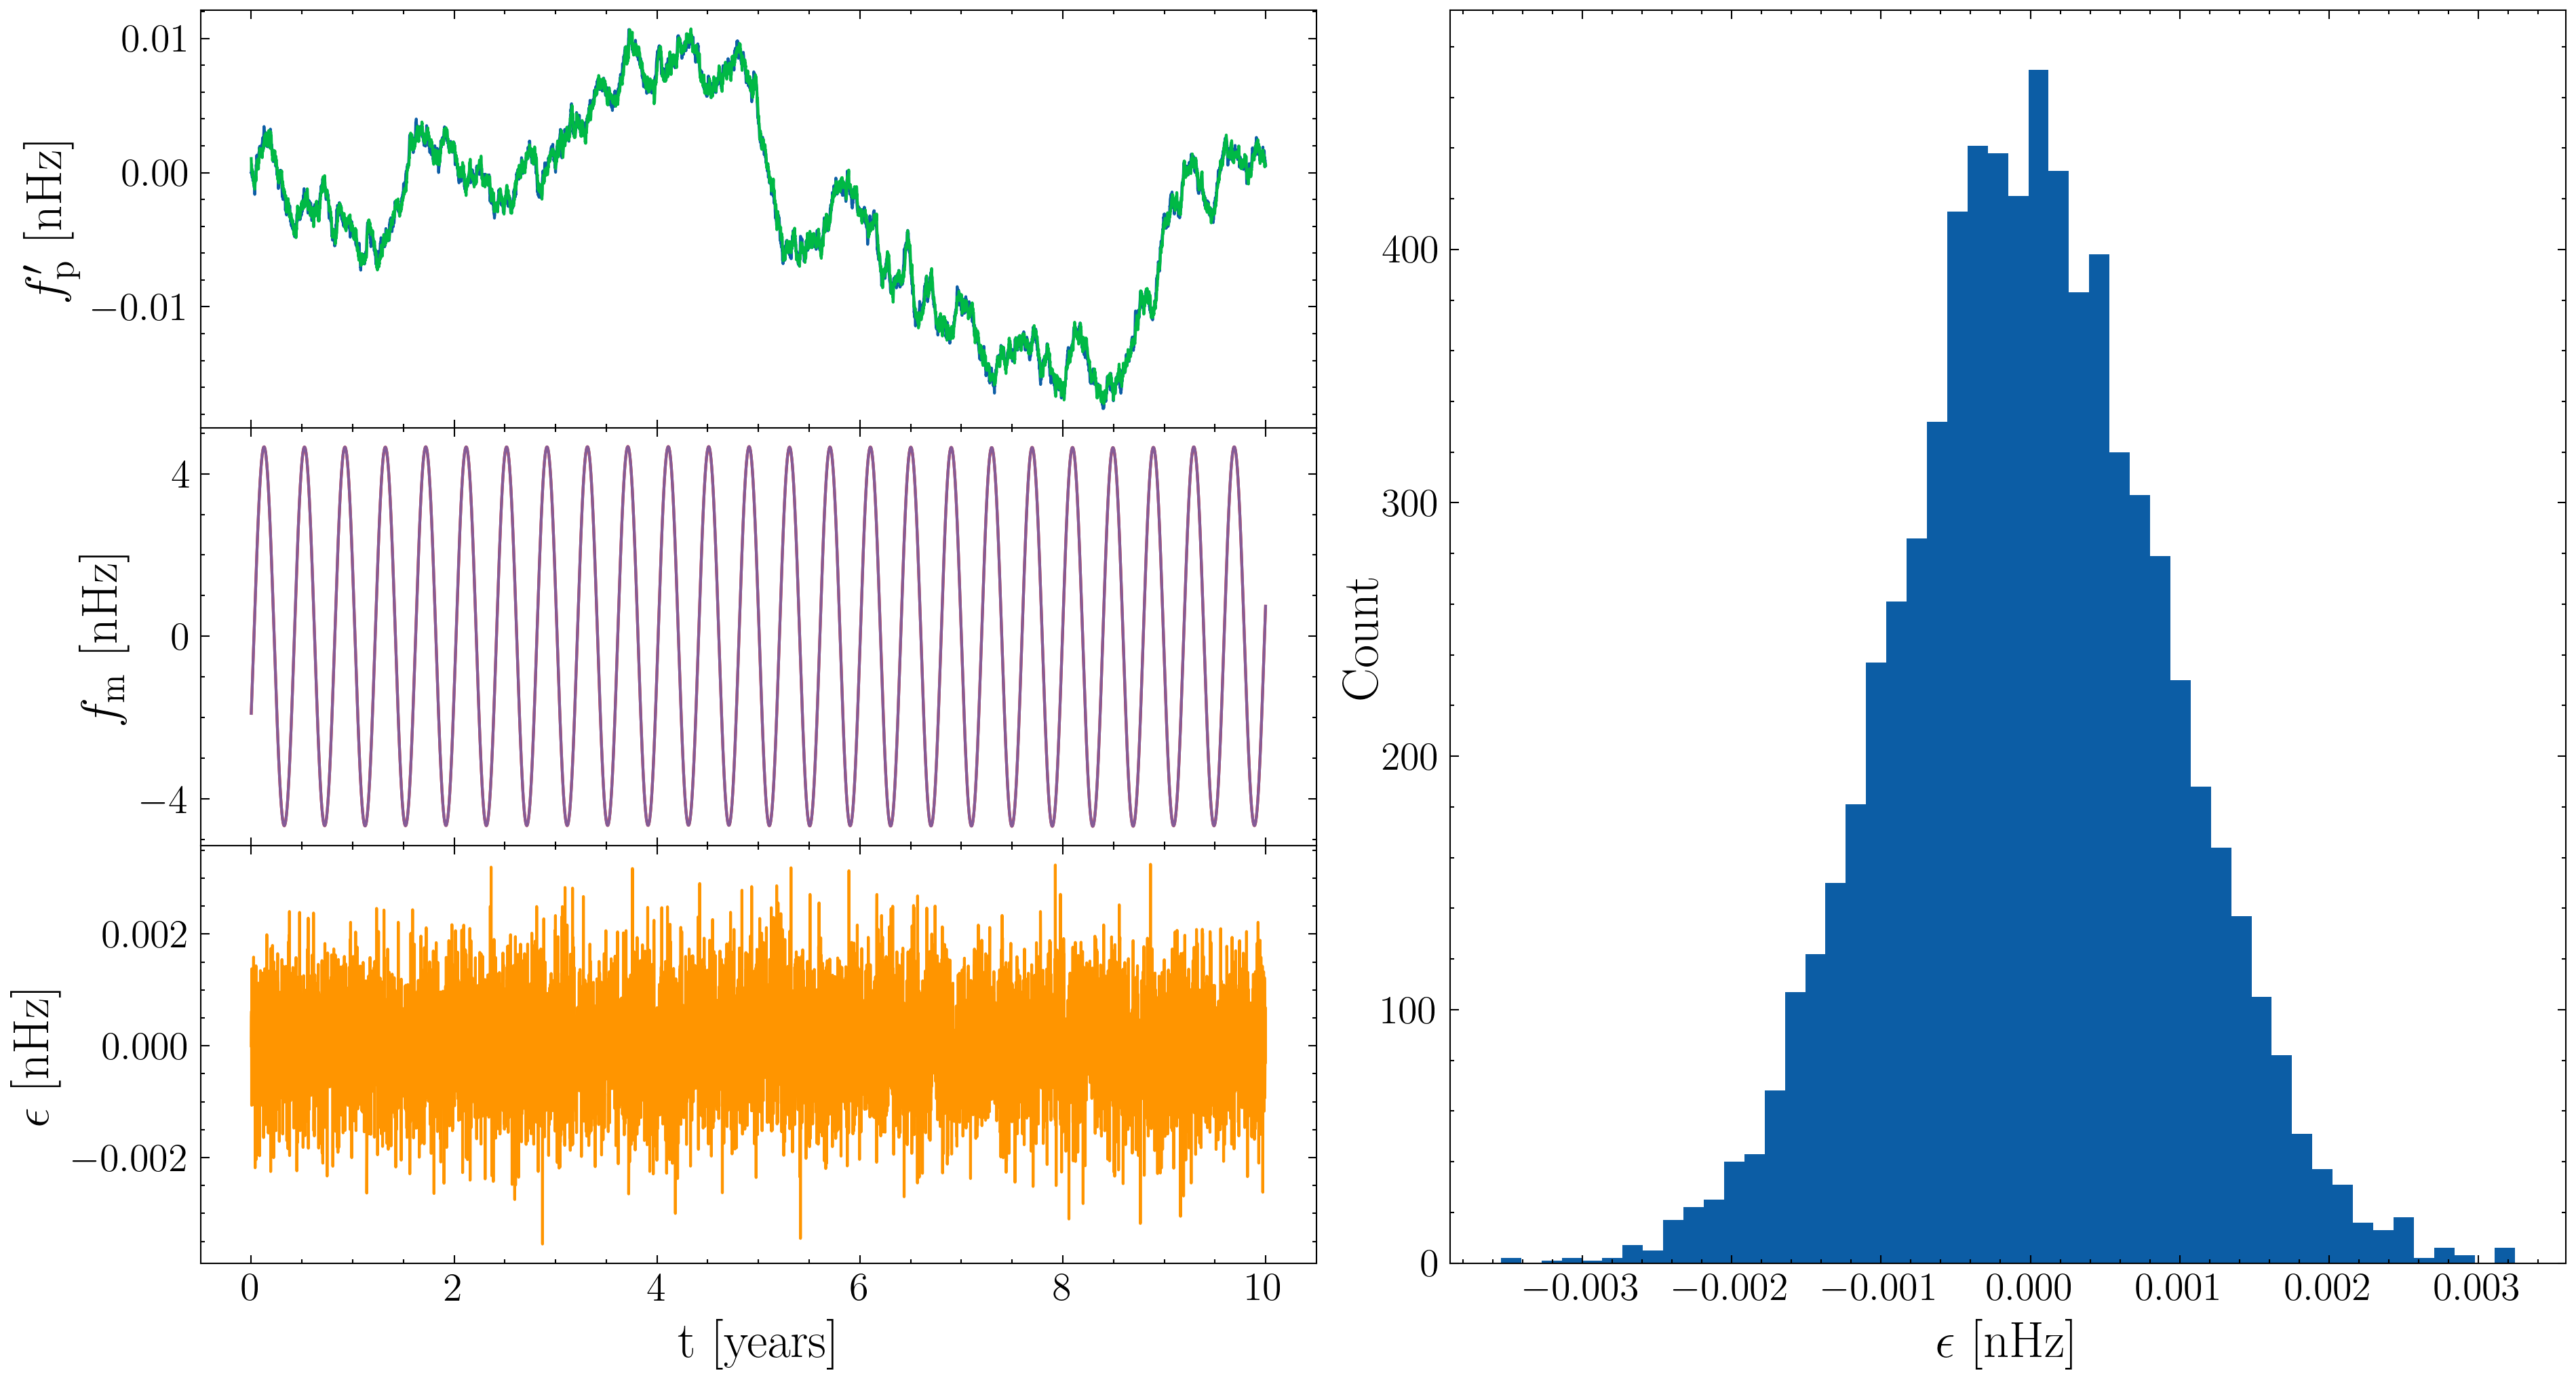
\includegraphics[width=\textwidth]{images/Kalman_example_true_params}
		\caption{Kalman filter using correct estimate of the static parameters, $\hat{\boldsymbol{\theta}} = \boldsymbol{\theta}$ }
		\label{fig:6MB_BFS}
	\end{subfigure} \newline 

	\begin{subfigure}[b]{1\textwidth}
		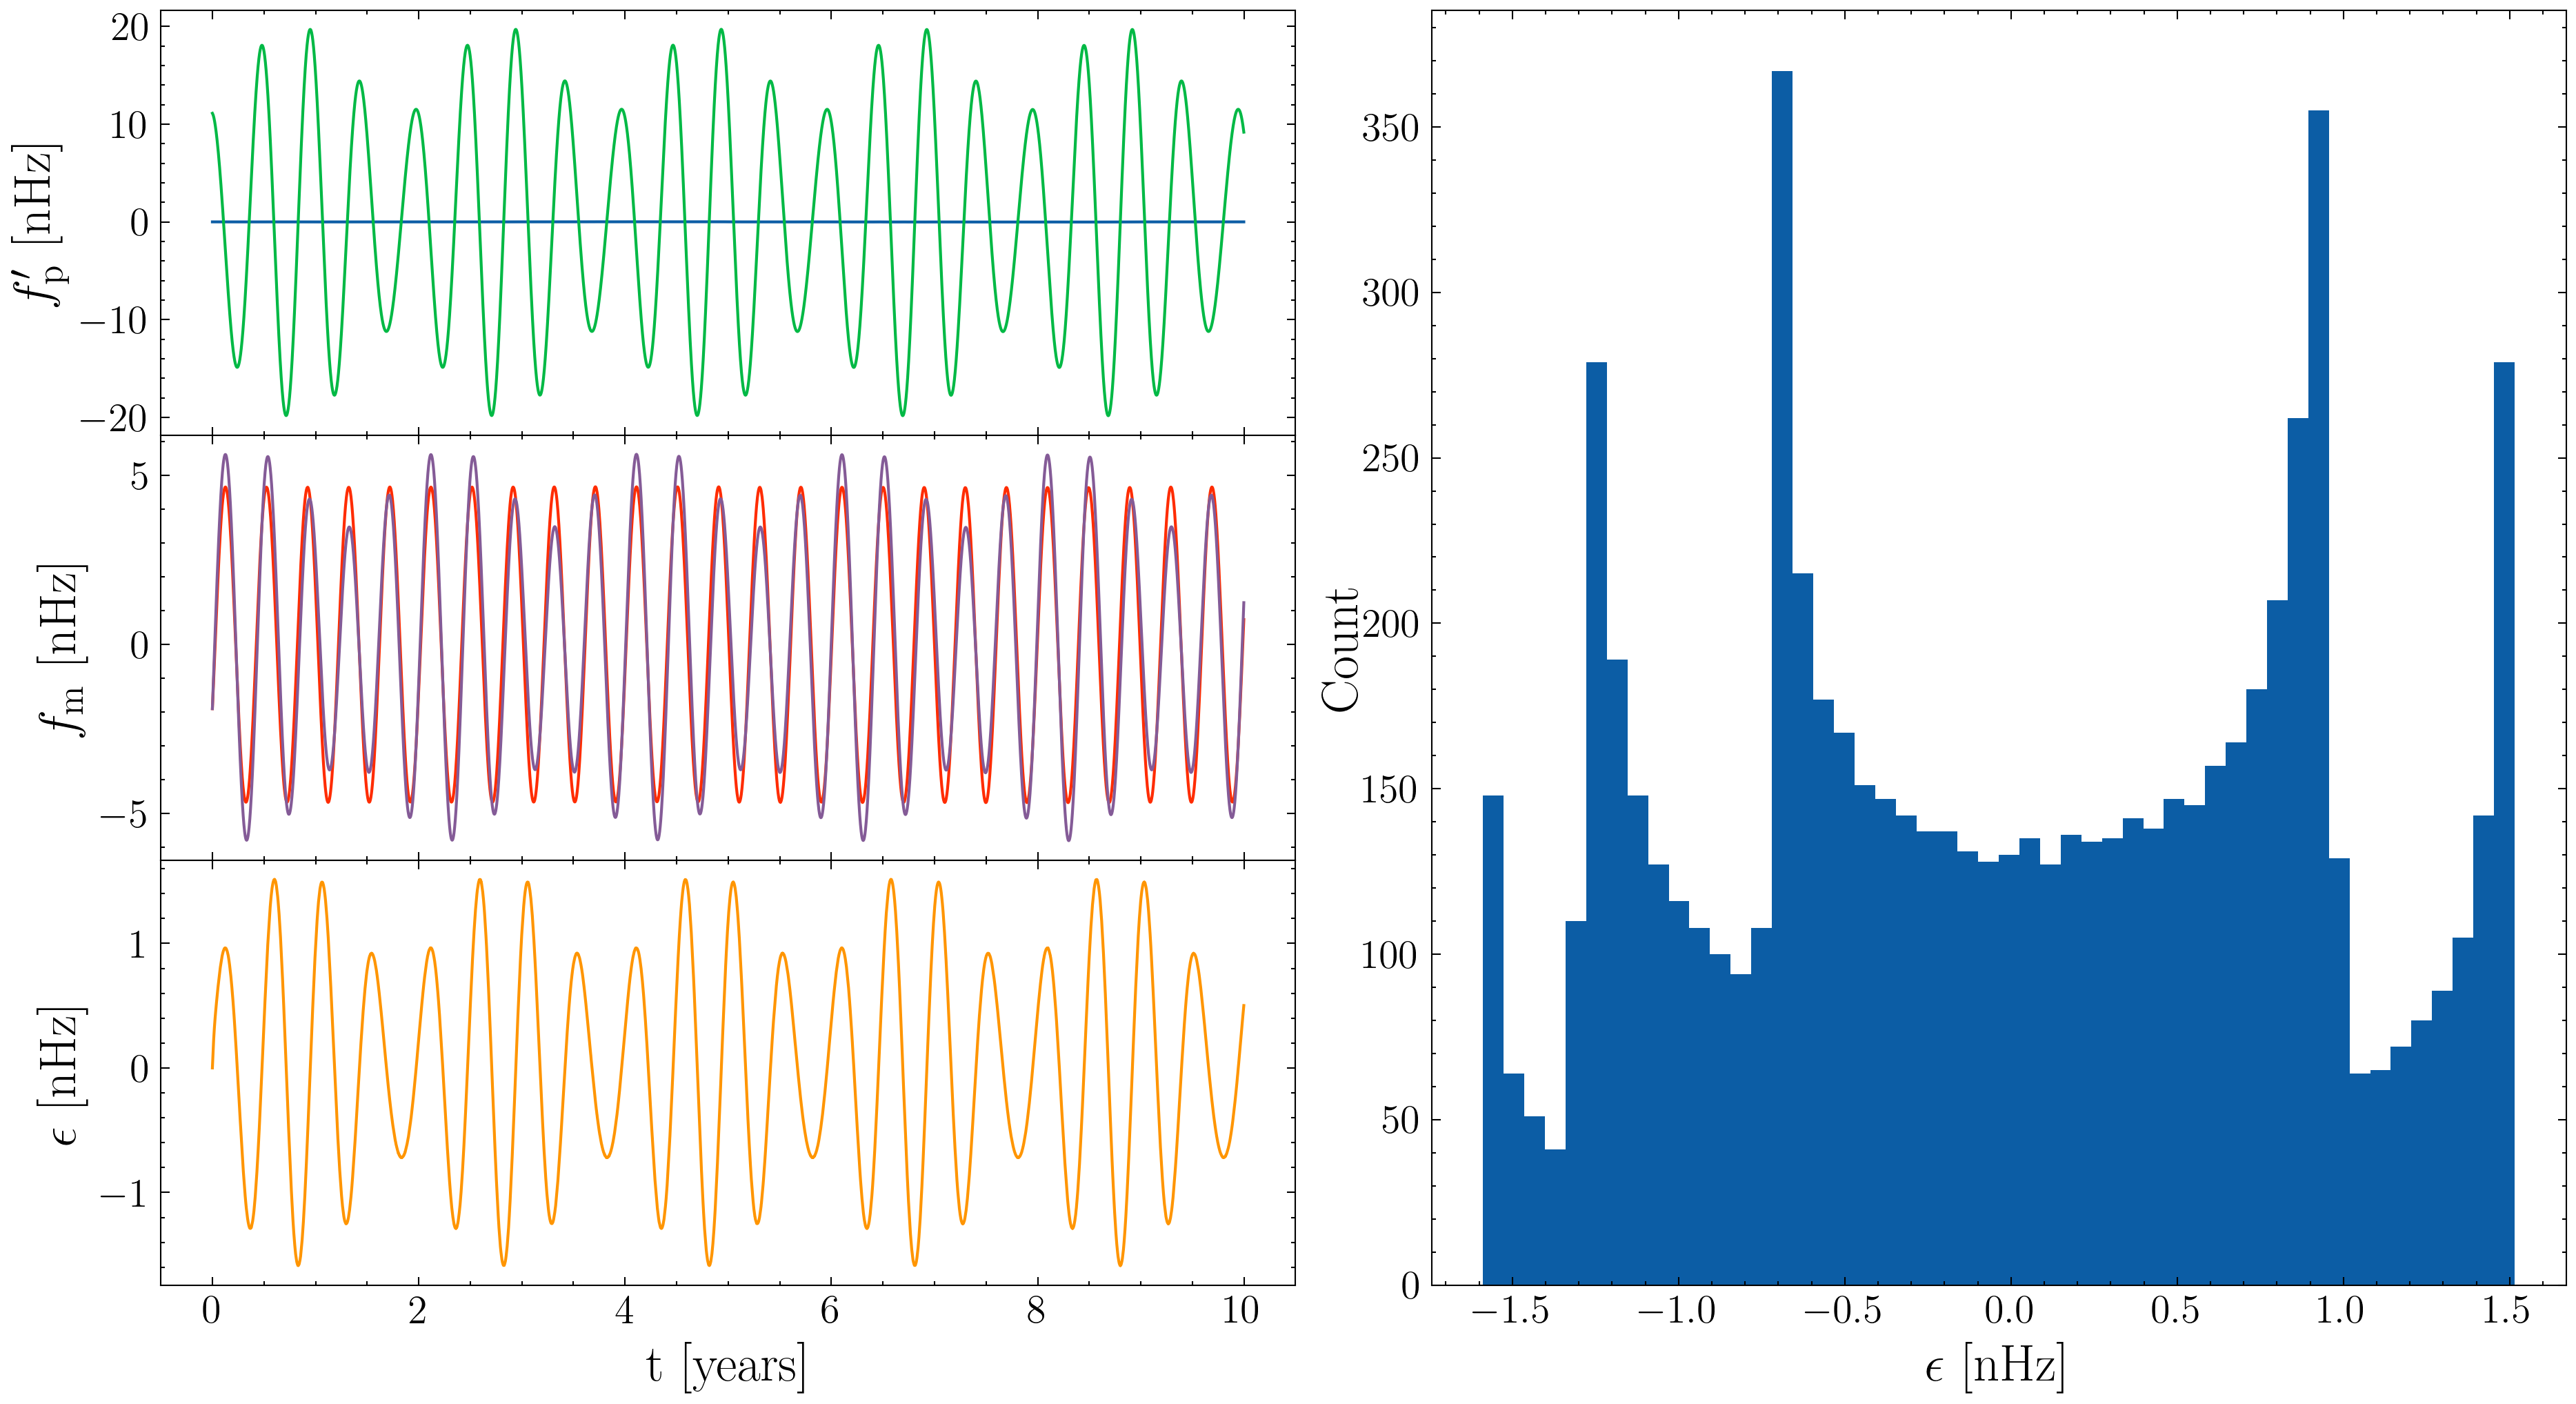
\includegraphics[width=\textwidth]{images/Kalman_example_wrong_params}
		\caption{Kalman filter using incorrect estimate of the static parameters, $\hat{\boldsymbol{\theta}} \neq \boldsymbol{\theta}$}
		\label{fig:25MB_bfs}
	\end{subfigure}
	\caption{Example application of a Kalman filter to estimate the intrinsic pulsar frequency state $f_{\rm p}(t)$ given a measured frequency $f_{\rm m}(t)$. We here plot the ephemeris subtracted state $f'_{\rm p}(t) = f_{\rm p}(t) - f_{\rm em} (t)$ to better illustrate the stochastic wandering of the pulsar frequency. In (a) the Kalman filter is run using identically correct estimates of the static system parameters, $\hat{\boldsymbol{\theta}} = \boldsymbol{\theta}$ and the state is estimated accurately. In (b) the Kalman filter is run with $\hat{\boldsymbol{\theta}} \neq \boldsymbol{\theta}$ and the state is not estimated accurately. The top left panels show the true pulsar state $f'_{\rm p}(t)$ (blue line) and the state estimated by the Kalman filter, $\hat{f'}_{\rm p}(t)$ (green line). The middle left panels show the true $f_{\rm m}(t)$ (red line) and the measured frequency estimated  by the Kalman filter, $\hat{f}_{\rm m}(t)$ (magenta). The bottom left panels show the residual or the innovation $\epsilon(t) =f_{\rm m}(t) - \hat{f}_{\rm m}(t)$. The right hand panels plot the distribution of the innovation over the total observation period.}
	\label{fig:four figures}
\end{figure*}

The Kalman filter \citep{Kalman1} is an algorithm for recovering the most likely evolution of a set of system state variables, $\boldsymbol{X}$, given some noisy measurements, $\boldsymbol{Y}$. It is a common technique in signal processing that has been applied successfully in neutron star astrophysics \citep[e.g.][]{Meyers2021,Melatos2023}. In this work we use the linear Kalman filter which assumes a linear relation between $\boldsymbol{X}$ and $\boldsymbol{Y}$. Whilst the measurement equation, Eq. \ref{eq:measurement}, is non-linear in the static parameters it is linear in the state and measurement variables, $f_{\rm p}^{(n)}$ and $f_{\rm m}^{(n)}$ respectively. Extension to non-linear problems is straightforward using either an extended Kalman filter \citep{zarchan2000fundamentals}, the unscented Kalman filter \citep{882463van} or the particle filter \citep{Simon10}. \newline 



The full set of Kalman recursions is presented in Appendix \ref{sec:kalman}. At each discrete timestep $i = 1, ... , M$, the Kalman filter returns an estimate of the state variables, $\hat{\boldsymbol{X}}_i$, and the covariance of those estimates, $\boldsymbol{P}_i$. The filter tracks the error in its predictions of $\boldsymbol{X}_i$ by projecting the state predictions back into measurement space, $\hat{\boldsymbol{X}}_i \mapsto \hat{\boldsymbol{Y}}_i$, via the measurement equation, Eq. \ref{eq:measurement}. The measurement predictions can then be compared aganst the true observed noisy measurements to get a residual $\boldsymbol{\epsilon}_i = \boldsymbol{Y}_i  - \hat{\boldsymbol{Y}}_i$, sometimes termed the ``innovation". The Kalman filter also calculates the uncertainty in $\boldsymbol{\epsilon}_i$ via the innovation covariance $\boldsymbol{S}_i = \langle \boldsymbol{\epsilon}_i \boldsymbol{\epsilon}_i^{\intercal} \rangle$. The Gaussian log-likelihood can then be calculated at each timestep:
\begin{eqnarray}
	\log \mathcal{L}_i =  -\frac{1}{2} \left (N \log 2 \pi + \log  \left | \boldsymbol{S}_i \right | + \boldsymbol{\epsilon}_i^{\intercal} \boldsymbol{S}_i^{-1}  \boldsymbol{\epsilon}_i \right ) \ ,
\end{eqnarray}
with the total log-likelihood simply the sum over all timesteps, i.e. 
\begin{eqnarray}
	\log \mathcal{L} =  \sum_{i=1}^{i=M} \log \mathcal{L}_i \ . \label{eq:likelihood}
\end{eqnarray}
For fixed data $\boldsymbol{Y}$, $\mathcal{L}$ is a function of the static parameters of the model, i.e. $\mathcal{L}$ = $\mathcal{L}(\boldsymbol{Y} | \boldsymbol{\theta})$. Similarly the estimates of the state and measurement variables, $\hat{\boldsymbol{X}}$ and $\hat{\boldsymbol{Y}}$, are also functions of $\boldsymbol{\theta}$. If the estimates of the system parameters, $\boldsymbol{\hat{\theta}}$ , that we pass to the Kalman filter are close to the true underlying parameters then the error in $\hat{\boldsymbol{X}}$, $\hat{\boldsymbol{Y}}$ is minimized and $\mathcal{L}$ is maximised. This is illustrated in Figure \ref{fig:6MB_BFS}; given a data timeseries of the measured pulsar frequency the Kalman filter is able to recover the evolution of the hidden state with high fidelity. The residuals correspond to random noise and are normally distributed. Conversely, if $\boldsymbol{\hat{\theta}}$ is not close to the true parameters then the filter is unable to recover the state evolution. This is demonstrated in Figure \ref{fig:25MB_bfs} where the Kalman filter was run with $\boldsymbol{\hat{\theta}}$ slightly perturbed away from the true values. In this case the filter cannot track the state variable accurately and the residuals are no longer Gaussian.


\subsection{Nested Sampling}\label{sec:nested_sampling}
We can use the likelihood returned by the Kalman filter, Eq \ref{eq:likelihood}, in conjunction with likelihood-based inference methods to estimate the posterior distribution of $\boldsymbol{\theta}$ by Bayes' Rule,
\begin{equation}
	p(\boldsymbol{\theta} | \boldsymbol{Y}) = \frac{\mathcal{L}(\boldsymbol{Y} | \boldsymbol{\theta}) \cdot \pi(\boldsymbol{\theta})}{\mathcal{Z}}
\end{equation}
where $\pi(\boldsymbol{\theta})$ is the prior distribution on $\boldsymbol{\theta}$ and $\mathcal{Z}$ is the marginalised likelihood, or evidence
\begin{equation}
	\mathcal{Z} = \int \mathcal{L}(\boldsymbol{Y} | \boldsymbol{\theta})  \pi(\boldsymbol{\theta}) d \boldsymbol{\theta} \ . \label{eq:model_evidence}
\end{equation}
In order to estimate the posterior distribution and the model evidence we use nested sampling \citep{Skilling} throughout this work. Nested sampling is an integration algorithm used for evaluating marginalised likelihood integrals, of the form given by Eq. \ref{eq:model_evidence}, that also returns samples from the posterior, $p(\boldsymbol{\theta} | \boldsymbol{Y})$. It does this by drawing a set of $n_{\rm live}$ live points from $\pi(\boldsymbol{\theta})$ and then iteratively replacing the live point with the lowest likelihood with a new live point drawn from $\pi(\boldsymbol{\theta})$, where the new live point is required to have a higher likelihood than the discarded point. The primary advantage of nested sampling is the ability to compute the evidence integral, which is key for model selection, and proves difficult without considerable extra cost for the usual Markov Chain Monte Carlo (MCMC) approaches. Nested sampling is also typically less computationally intensive than MCMC and can handle multi-modal problems \citep{Ashton2022}. For these reasons, it has enjoyed widespread adoption in the physical sciences, particularly within the cosmological community \citep{Mukherjee2006,Feroz2008,Handley2015}, but has also commonly been applied in astrophysics \citep{UltraNest2021}, particle physics \citep{proceedings2019033014} and materials science \citep{2009arXiv0906materials}. For a review of nested sampling we refer the reader to \cite{Buchner2021} and \cite{Ashton2022}. Multiple nested sampling algorithms and computational libraries exist. \citep[e.g.][]{Feroz2008,Feroz2009,Handley2015,dynesty2020,UltraNest2021}. For gravitational astrophysics it is common to use the \texttt{dynesty} sampler \citep{dynesty2020} via the \texttt{Bilby} \cite{bilby.507.2037A} front-end library. We  follow this precedent and use \texttt{Bilby} for all nested sampling Bayesian inference in this work. The primary tunable parameter in nested sampling is $n_{\rm live}$, where a greater number of live points is advantageous for large parameter spaces and multi-modal problems, whilst the uncertainties in the evidence and the posterior scale as $\mathcal{O}(1/\sqrt{n_{\rm live}})$. However the computational runtime scales as $\mathcal{O}(n_{\rm live})$ and so one must make a trade-off between uncertainty and runtime. \cite{Ashton2022} offer a rule-of-thumb where the minimum number of live points should be greater than the number of static parameters. The results presented in this work are generally robust to the choice of $n_{\rm live}$, subject to the requirement of $n_{\rm live} > 7 + 5N$. We take $n_{\rm live} = 500$ for all results presented in this work. 

%See https://arxiv.org/pdf/2102.12478.pdf for a good NS explanation


\subsection{Model selection}\label{sec:model_selection}
The evidence integral,$\mathcal{Z}$, returned by nested sampling is the probability of the data $\boldsymbol{Y}$ given a particular model $\mathcal{M}_i$. This enables us to compare competing models via a Bayes factor,
\begin{equation}
	\beta = \frac{\mathcal{Z}(\boldsymbol{Y} | \mathcal{M}_1)}{\mathcal{Z}(\boldsymbol{Y} | \mathcal{M}_0)} \ . \label{eq:bayes}
\end{equation}
Throughout this work we take $\mathcal{M}_1$ to be the complete model defined in Section \ref{sec:model}. $\mathcal{M}_0$ is our null model that assumes there is no GW in the data. This is equivalent to setting $g^{(n)}(t)=1$ in Equation \ref{eq:g_func}, \ref{eq:g_func_trig}. The Bayes factors we quote in this work therefore quantify whether the data supports evidence for a GW compared to there being no GW signal present.



\section{Tests with synthetic data} \label{sec:testing}
In this section we use synthetic data to test the ability of our method to detect the presence of a GW in noisy data and recover the static parameters, $\boldsymbol{\theta}$. In Section \ref{sec:synth_data} we discuss how the synthetic data is generated, including the construction of an artificial PTA. In Section \ref{sec:rep_example} we generate synthetic data for a single representative example SMBHB system and apply our method to estimate $\boldsymbol{\theta}$ and calculate the statistical evidence for a GW in the data via the Bayes factor. In this section we also explore how the detectability of the system changes for different strain magnitudes, $h_0$ and the performance of the method for different realisations of the system noise. In Section \ref{sec:parameter_space} we move beyond a single example system and test our method across a broader parameter space. In Section \ref{sec:bias} we discuss biases that are evident in some of the parameter estimates.

\subsection{Synthetic data generation} \label{sec:synth_data}

\subsubsection{Constructing a synthetic PTA}\label{sec:synt_pta}

\begin{figure}
	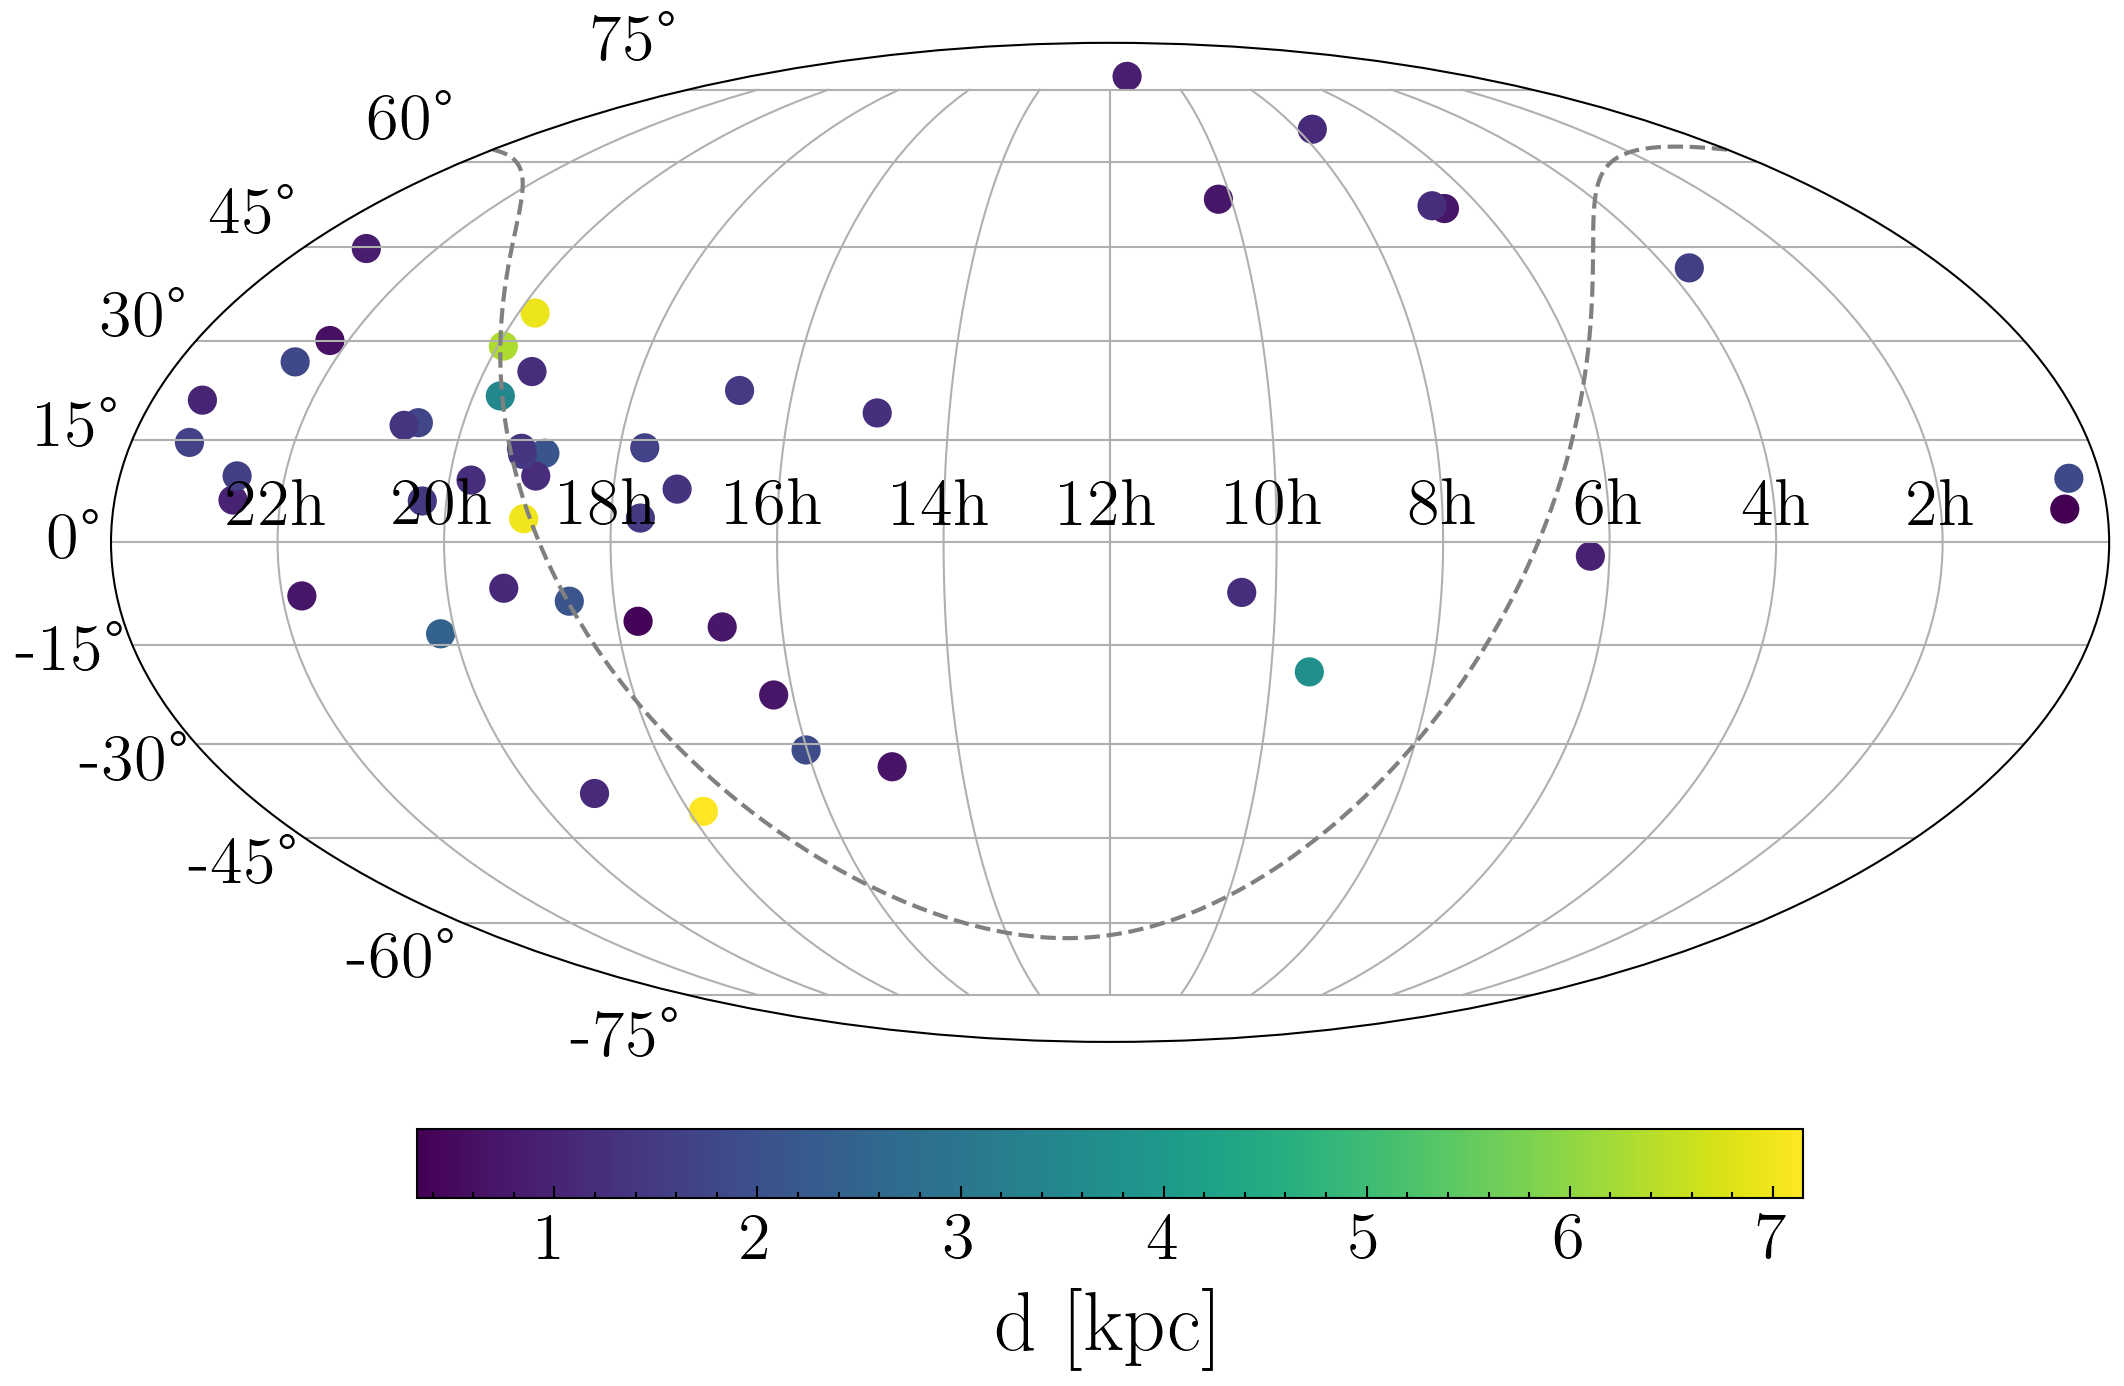
\includegraphics[width=\columnwidth]{images/pulsar_distribution}
	\caption{Spatial distribution of 47 pulsars from the 12.5 year NANOGrav data release that make up the synthetic PTA used in this work. The pulsar distances relative to the observer are also indicated, with the majority of pulsars having a distance $\sim 1$ kpc. The grey dashed line denotes the Galactic plane.}
	\label{fig:pulsar_distrib}
\end{figure}

For this work we generate representative synthetic data as follows. We first specify a set of pulsars to make up our artificial PTA. We take the 47 pulsars that make up the 12.5 year NANOGrav PTA \citep{2020ApJ...905L..34A}. For each pulsar we obtain the sky location (which defines the vector $\boldsymbol{q}^{n}$), the distance, the barycentric rotation frequency - which we identify with $f_{\rm em}^{(n)} (t_1)$ -  and the time derivative of the the barycentric rotation frequency - which we identify with $\dot{f}_{\rm em}^{(n)} (t_1)$. The spatial distribution and the distances of the pulsars used for this artificial PTA are shown in Fig \ref{fig:pulsar_distrib}. The data is acquired via the Australia Telescope National Facility pulsar catalogue \citep{Manchester2005} using the \texttt{psrqpy} package \citep{psrqpy}. The remaining unspecified pulsar parameters are $\gamma^{(n)}$ and $\sigma^{(n)}$. We discussed in Section \ref{sec:psr_frequency} how the quantity $[\sigma^{(n)}]^2 /\gamma^{(n)} $ sets the amplitude of the characteristic root mean square fluctuations in $f_p^{(n)}(t)$. Typically the mean reversion timescale $[\gamma^{(n)}]^{-1} >> T_{\rm obs}$ \citep{Vargas}, whilst $[\sigma^{(n)}]^2$ varies between individual pulsars. For this work we fix $\gamma^{(n)} = 10^{-13}$ s$^{-1}$ for all $n$. In order to set a physically reasonable value for $[\sigma^{(n)}]^2$ we use two complementary approaches. The first approach uses the empirical timing noise model from \cite{Shannon2010ApJ...725.1607S} where the standard deviation in the pulsar TOA is given by:
\begin{align}
	\ln \left(\frac{\sigma_{\rm TOA}^{(n)}}{\mu s} \right)&= \ln \alpha_1 +  \alpha_2 \ln f_{\rm p}^{(n)} + \alpha_3 \ln \left(\frac{\dot{f}_{\rm p}^{(n)}}{10^{-15} \text{s}^{-2}} \right) \nonumber \\ 
	&+ \alpha_4 \ln \left( \frac{T}{ 1 \text{ year}} \right) \ , \label{eq:sigmap}
\end{align}
where $T$ is the length of the observation span and for MSPs $\ln \alpha_1 \sim -20 $, $\alpha_2 \sim 1$, $\alpha_3 \sim 2$ and $\alpha_4 \sim 2.4$. Throughout this work we assume that all pulsars are observed with a weekly cadence i.e. $T = 1$ week. The frequency noise parameter can then be calculated for each pulsar where the standard deviation in the pulsar TOA can be related to the standard deviation in the pulsar frequency as 
\begin{eqnarray}
	\sigma^{(n)} \sim \sigma_{\rm TOA}^{(n)} \frac{f_{\rm p}^{(n)}}{T} \ . \label{eq:sigmap_f}
\end{eqnarray}
For our synthetic NANOGrav PTA, the median $\sigma^{(n)}$ calculated in this way is $ = 4.28 \times 10^{-21} $ s. \newline 


As a sanity check, we can also calculate $\sigma^{(n)}$ using a complementary numerical approach to the empirical best-fit model outlined above. We can directly solve the state equation Eq. \ref{eq:spinevol} numerically using the \texttt{baboo} package \footnote{\url{https://github.com/meyers-academic/baboo}} so as to obtain a synthetic phase solution,
\begin{eqnarray}
	\phi^{(n)}(t) = \int_0^t dt' f^{(n)}_{\rm p}(t') \ ,
\end{eqnarray}
and generate TOAs and phase residuals. We calibrate the noise amplitude $\sigma^{(n)}$  to generate phase residuals that qualitatively resemble empirical phase residuals measured from real pulsars. We obtain empirical phase residuals from the UTMOST pulsar timing program \citep{UTMOST} from the  Molonglo Observatory Synthesis Telescope \citep{Bailes2017PASA...34...45B}. For the purposes of validating the $\sigma^{(n)}$ inferred from Eq \ref{eq:sigmap_f}, it is sufficient at this stage to simply compare the synthetic and real phase residuals visually. Whilst it would also be possible to e.g. define some quantitative loss function (e.g. mean-squared error) between the two solutions and solve the optimisation problem to infer $\sigma^{(n)}$, for our purposes this is excessive. It is satisfactory to simply qualitatively compare the two solutions as a useful sanity check. We emphasise that we are not overly concerned with calculating the maximally accurate values for $\sigma^{(n)}$, but instead some reasonable values for constructing representative synthetic data. This approach of generating synthetic phase solutions and visually comparing with empirical solutions is also followed in \cite{Vargas}. In Figure \ref{fig:qualitative_compare} we compare the synthetic and empirical residuals for the NANOGrav pulsar J0030+0451. We can see that the synthetic and empirical residuals are qualitatively similar.
\begin{figure}
	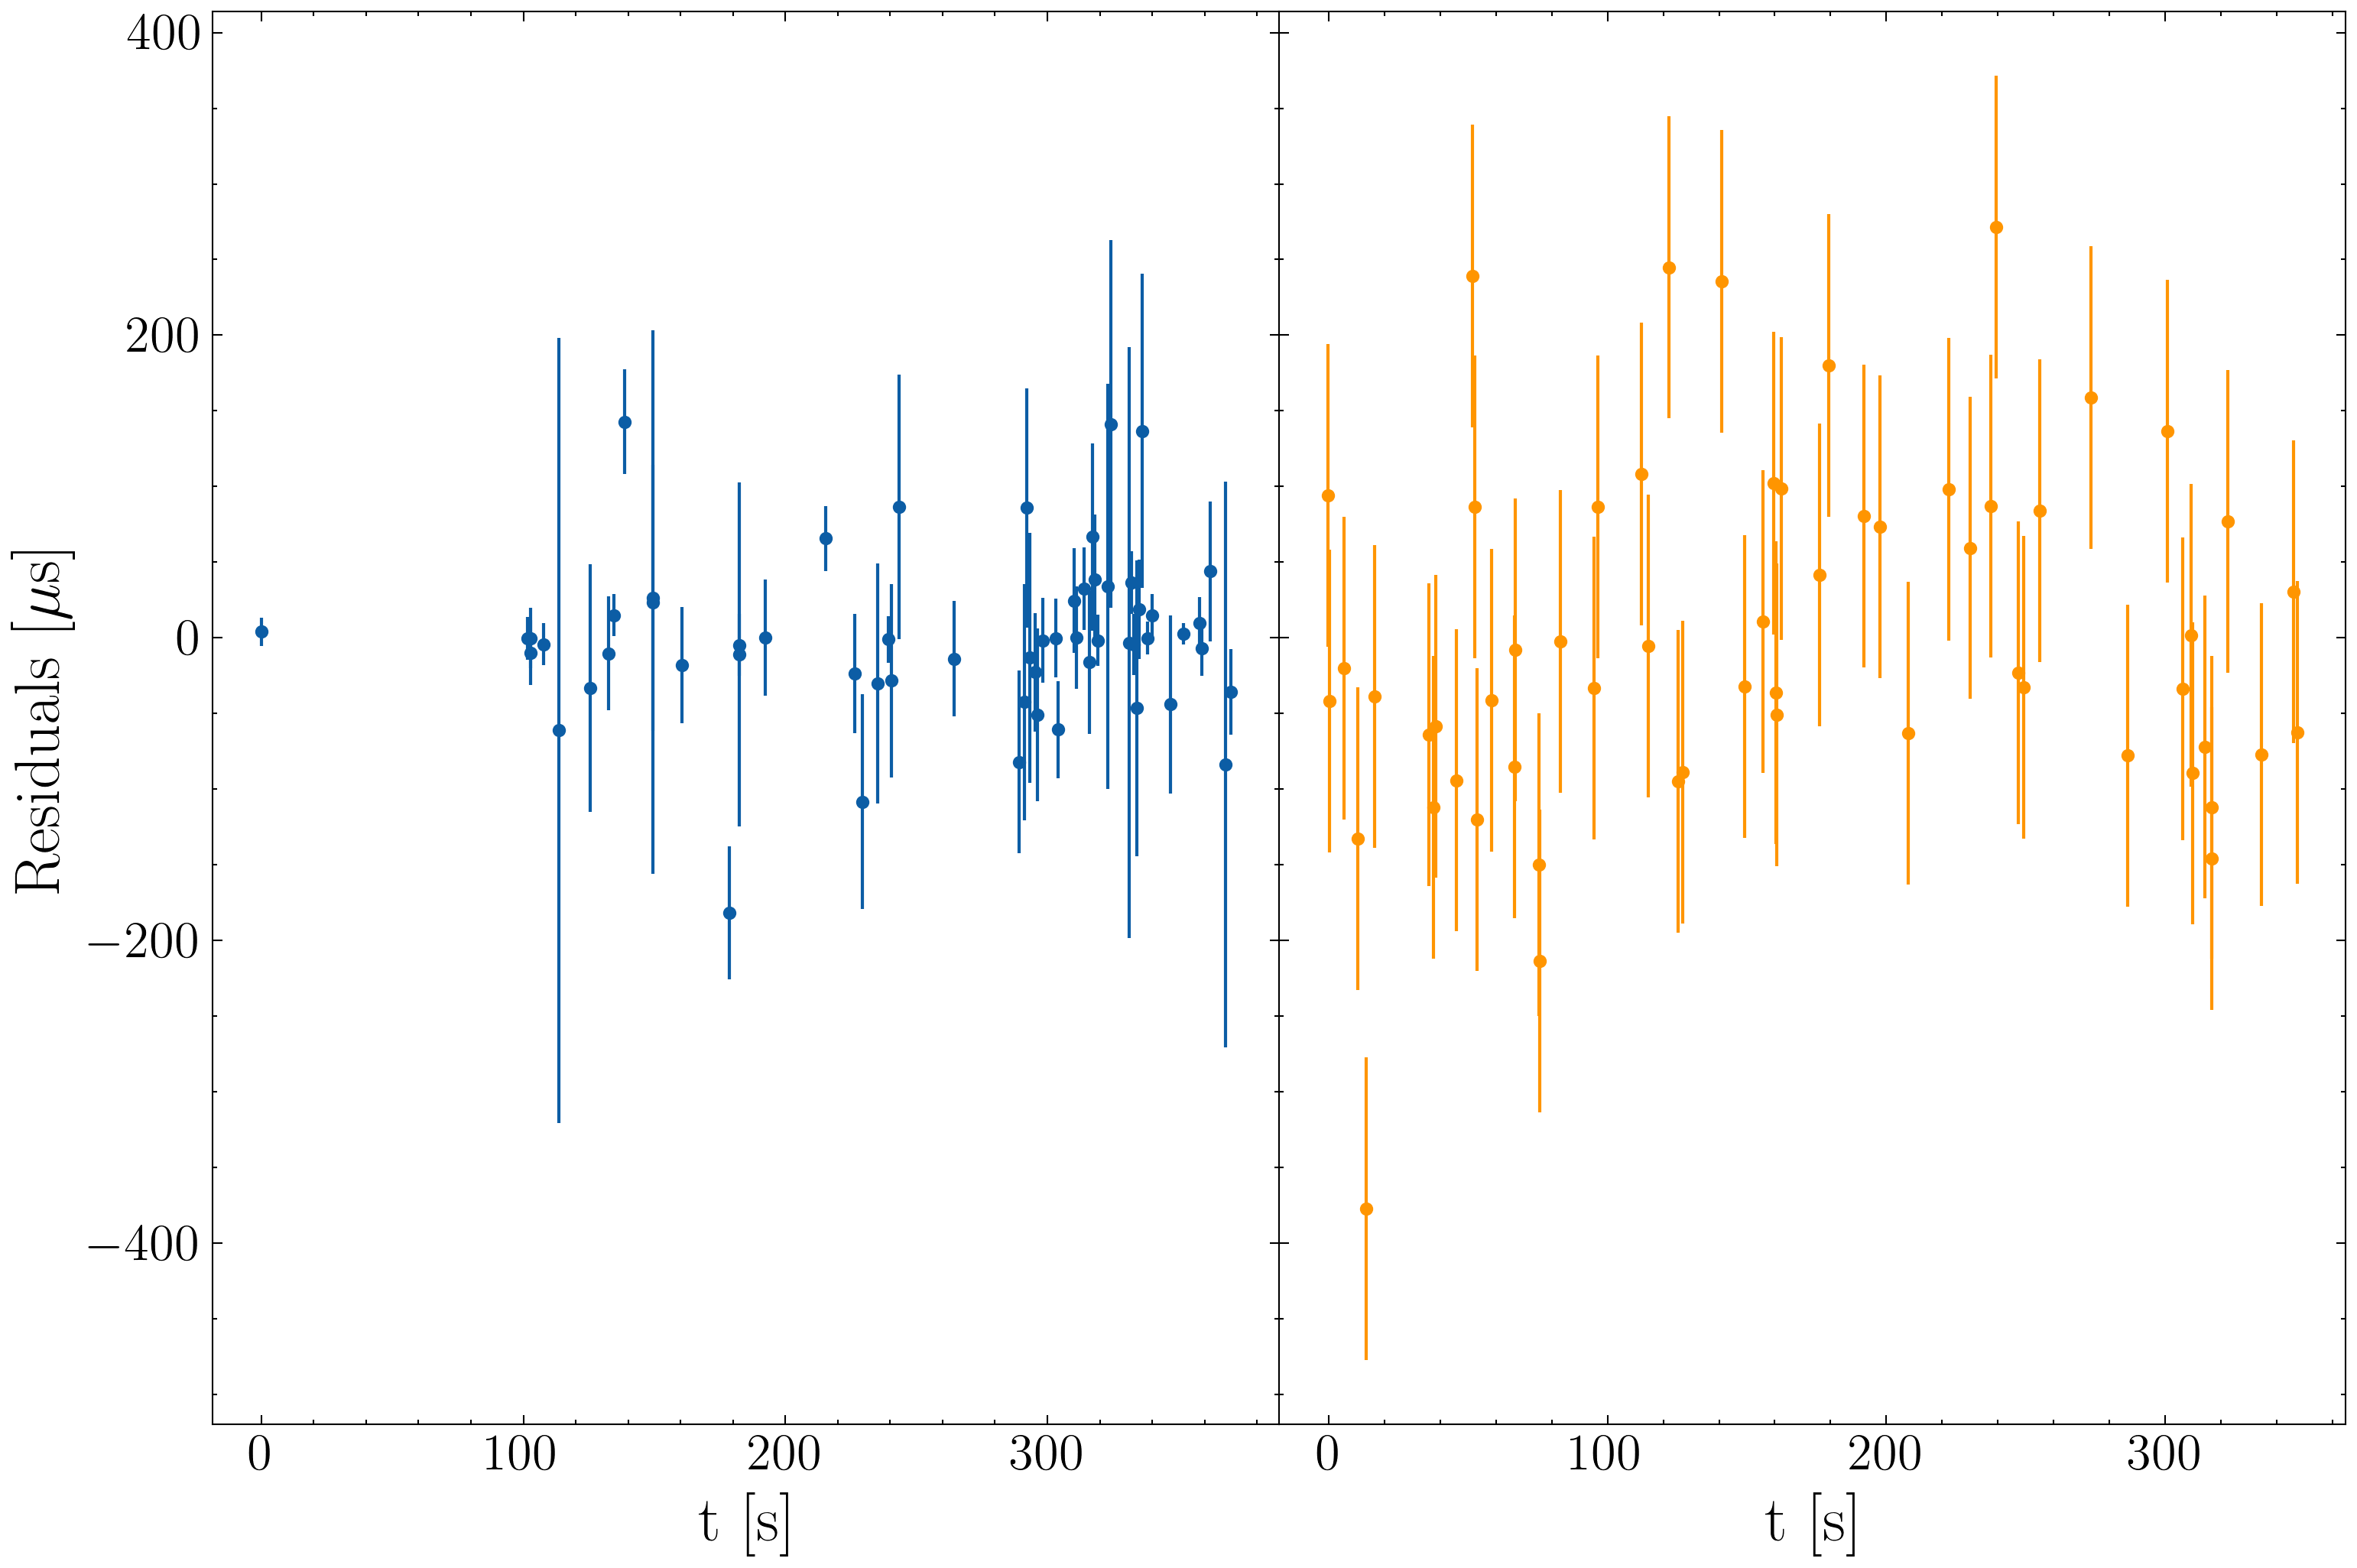
\includegraphics[width=\columnwidth]{images/example_residuals_plot}
	\caption{Actual (left panels) and synthetic (right panels) phase residuals for 3 NANOGrav pulsars. The actual residuals are obtained via the NANOGrav 12.5 year data release \citep{nanograv_narrowband_DR}. The synthetic residuals are generated by numerically solving Eq. \ref{eq:spinevol} with $\gamma^{(n)} = 10^{-13}$ and $\sigma^{(n)}$ inferred from Eqs. \ref{eq:sigmap}, \ref{eq:sigmap_f}. For all pulsars the two solutions are qualitatively similar, with comparable magnitudes in the residuals. \textcolor{red}{TK: potential sinusoidal feature? Need to discuss with Andres re use of baboo.}}
	\label{fig:qualitative_compare}
\end{figure}
\subsubsection{Synthetic data generation}
We generate $N$ synthetic noisy timeseries - one for each pulsar - as follows:

\begin{enumerate}
	\item Integrate the state equations, Eq \ref{eq:spinevol}- \ref{eq:xieqn} numerically for the synthetic PTA described in Section \ref{sec:synt_pta}.
	\item Map from state space to measurement space via the measurement equation, Eq. \ref{eq:measurement}
	\item Add zero-mean Gaussian measurement noise to each timeseries, i.e. $f_{\rm m} ^{(n)} + N_{\rm f}^{(n)}$ where 	$\langle N_{\rm f}(t) N_{\rm f}(t') \rangle = \sigma_{\rm m}^2 \delta(t - t')$ for measurement noise covariance $\sigma_{\rm m}^2$.
\end{enumerate}
Equations \ref{eq:spinevol}- \ref{eq:xieqn} are solved by a Runge-Kutta It$\hat{\text{o}}$ integrator implemented in the \texttt{sdeint} python package \footnote{\url{https://github.com/mattja/sdeint}}. The static pulsar parameters  $\boldsymbol{\theta}_{\rm psr}$ are completely specified by our construction of the synthetic PTA outlined in Section \ref{sec:synt_pta}. For this work we consider all pulsars to be observed for $T_{\rm obs} =10$ years, uniformly sampled with a weekly cadence. The measurement noise can be approximately related to the uncertainty in the pulse TOA, $\sigma_{\rm TOA}$, as
\begin{equation}
	\sigma_{\rm m} \sim f_{\rm p}^{(n)} \frac{\sigma_{\rm TOA}}{\text{cadence}} \ . 
\end{equation}
For a millisecond pulsar with $f_{\rm p}^{(n)} \sim 100$ Hz observed with a weekly cadence and $\sigma_{\rm TOA} \sim 1 \mu$s this gives $\sigma_{\rm m} \sim 10^{-10}$, whilst the very best pulsars might have $\sigma_{\rm TOA} \sim 10 $ ns or $\sigma_{\rm m} \sim 10^{-12}$. Throughout this work we fix $\sigma_{\rm m} = 10^{-11}$ and take it to be known \textit{a priori} rather than a parameter to be inferred. Note that $f_{\rm m} ^{(n)}$ is modified by a different realisation of the measurement noise for each pulsar; whilst for our construction every pulsar is sampled at the same time and so would experience the same realisation of the noise, in actual pulsar astronomy different pulsars will be sampled at different times and so subject to different noise realisations. \newline 

In practice, in order to avoid numerical precision issues that arise when solving Eq \ref{eq:spinevol}- \ref{eq:xieqn} $\left ( \text{since } \sigma^{(n)} \ll f_{\rm p}^{(n)} \right)$ we first ``heterodyne" our state by subtracting the deterministic frequency evolution, equivalent to a change of variables:
\begin{equation}
	f_{\rm p}^{\prime (n)} = f_{\rm p}^{(n)} - f_{\rm em}^{(n)}
\end{equation}  
We similarly heterodyne the measurement variable 
\begin{equation}
	f_{\rm m}^{\prime (n)} = f_{\rm m}^{(n)} - f_{\rm em}^{*(n)}
\end{equation}
where $ f_{\rm em}^{*(n)}$ is a guess of the deterministic spin-down based on the pulsar ephemeris. For synthetic data we can set $ f_{\rm em}^{*(n)} = f_{\rm em}^{(n)}$ but this is not true generally for real-world observations since the spin-down ephemeris is only known approximately, not exactly. The measurement equation Eq. \ref{eq:measurement} that relates the state and measurement variables is then updated as 
\begin{equation}
	f_{\rm m}^{\prime (n)}(t) = f_{\rm p}^{\prime (n)}(t-d) g^{(n)}(t) -  f_{\rm em}^{(n)}(t-d)\left[ 1-g^{(n)}(t)\right]
	\label{eq:measurement_cov}
\end{equation}
We emphasise that this change of variables is simply a convenient scaling to bring our numerical values into a reasonable dynamic range without having to use extended numerical floating point formats (e.g. long double, quadruple). It does not remove any degrees of freedom of the formulation. In particular both $f_{\rm em}^{(n)}(t_1)$
and $\dot{f}_{\rm em}^{(n)}(t_1)$ remain static parameters of the model, but now appear in the measurement equation rather than the state equation.


\subsection{Representative example}\label{sec:rep_example}
We initially characterise our method with a single example of a PTA which is perturbed by a GW from an individual quasi-monochromatic SMBHB source. The static GW source parameters $\boldsymbol{\theta}_{\rm gw}$ used for this injection are selected arbitrarily, subject to being astrophysically reasonable and representative. The injected $\boldsymbol{\theta}_{\rm gw}$ are summarised in the ``Injected Values" column of Table \ref{tab:parameters_and_priors}. The static pulsar parameters $\boldsymbol{\theta}_{\rm psr}$ are as described in Section \ref{sec:synt_pta} and are also shown in Table \ref{tab:parameters_and_priors}. 

\subsubsection{Prior distributions}\label{sec:priors}

For the Bayesian methods used in this work, one must select reasonable priors, $\pi(\boldsymbol{\theta})$, for the complete set complete of static parameters. For $\pi(\boldsymbol{\theta}_{\rm gw})$ we choose standard non-informative priors \citep[e.g.][]{Bhagwat2021} as summarised in Table \ref{tab:parameters_and_priors}. The choice of $\pi(\boldsymbol{\theta}_{\rm psr})$ requires some additional discussion. \newline 


The parameters which govern the deterministic evolution of the pulsar spin frequency, $f_{\rm em}^{(n)} (t_1)$,$\dot{f}_{\rm em}^{(n)} (t_1)$ are well-determined by existing radio timing observations. We can identify $f_{\rm em}^{(n)} (t_1)$,$\dot{f}_{\rm em}^{(n)} (t_1)$ with the pulsar  barycentric rotation frequency and the time derivative of barycentric rotation frequency quoted by pulsar observation catalogues. For the 12.5 year NANOGrav pulsars the mean error in the barycentric rotation frequency is $\sim 1.1 \times 10^{-11}$ Hz, and in the time derivative of barycentric rotation frequency is $\sim 1.29 \times 10^{-19}$ s $^{-2}$. These mean errors are skewed by a minority of pulsars which are less well timed; the median error in  the barycentric rotation frequency is $\sim 7 \times 10^{-13}$ Hz, and in the time derivative of barycentric rotation frequency is $\sim 1.8 \times 10^{-20}$ s $^{-2}$. Whilst it is then clear that $f_{\rm em}^{(n)} (t_1)$,$\dot{f}_{\rm em}^{(n)} (t_1)$ are typically measured with very high precisions, for this work we adopt a broader uniform prior, $\pm 1 \%$ either side of the true value. In this way we can test how well our method performs without requiring exceptionally precise and accurate measurements of the pulsar parameters to be made \textit{a priori}. Instead we consider the pulsar parameters similarly to the GW source parameters and estimate them optimally within a consistent framework. Leaving the priors looser in this way allows us to subject our method to a more stringent test and confirm that we still estimate GW parameters without highly accurate initial estimates of $f_{\rm em}^{(n)} (t_1)$,$\dot{f}_{\rm em}^{(n)} (t_1)$. \newline 



The pulsar distances $d^{(n)}$ are typically not as well constrained as $f_{\rm em}^{(n)} (t_1)$,$\dot{f}_{\rm em}^{(n)} (t_1)$, with uncertainties typically on the order of $\sim 10 \%$ \citep{Arzoumanian2018ApJS..235...37A,Yao2017}. However for this work, whilst the pulsar distance is used when generating synthetic data, as discussed in Section \ref{sec:parameter_estim} the pulsar distance is not used for our inference model and so we do not need to set a prior on $d$. Similarly we do not set a prior on $\gamma^{(n)}$; since $[\gamma^{(n)}]^{-1} >> T_{\rm obs}$ this means that $\gamma^{(n)}$ is effectively ``unobservable" over the decadal timescales that we are interested in. That is, for $T_{\rm obs}$ =10 years the solution of Eq \ref{eq:spinevol} is effectively independent of the choice of $\gamma^{(n)}$ as long as the condition $[\gamma^{(n)}]^{-1} >> T_{\rm obs}$ is satisfied. It is therefore sufficient to consider $\gamma^{(n)}$ to be known \textit{a priori} and set it at its true injected value. We briefly explored setting an uninformative prior on $\gamma$ over e.g. LogUniform($10^{-10}, 10^{-15}$) as well as setting $\gamma^{(n)}$ at some fixed value away from the true injected value (e.g. set $\gamma^{(n)} = 10^{-14} \text{s}^{-1}$ rather than $10^{-13} \text{s}^{-1}$) but the results are unchanged. The majority of pulsars in our synthetic PTA have $\sigma^{(n)} \sim 10^{-20} - 10^{-22}$ as calculated from Eqs. \ref{eq:sigmap}, \ref{eq:sigmap_f}. For these pulsars we set an uninformative broad prior of LogUniform($10^{-19}, 10^{-23}$). The single exception is PSR J1939+2134 which has a particularly large $\dot{f}_{\rm p}^{(n)}$ compared to the other pulsars in the array and so $\sigma \sim 10^{-16}$. For PSR J1939+2134 we set the prior at LogUniform($10^{-15}, 10^{-17}$). \newline

Since we are not setting priors on $\gamma$ or $d$ this reduces the dimensionality of the parameter space to $7 + 3N$. We use the notation $\boldsymbol{\theta}_{\rm psr, reduced}$ to refer to the reduced parameter space. Explicitly, 
\begin{equation}
	\boldsymbol{\theta}_{\rm psr, reduced} = \left \{ f_{\rm em}^{(n)}(t_1),\dot{f}_{\rm em}^{(n)}(t_1),\sigma^{(n)}\right\}_{1\leq n \leq N} \ .
\end{equation}
All the injected static parameters and their corresponding priors for this representative example are summarised in Table \ref{tab:parameters_and_priors}.
\begin{table}
	\centering
	\resizebox{\columnwidth}{!}{%
	\renewcommand{\arraystretch}{1.5} % Default value: 1
	\begin{tabular}{lccll}
		\toprule
		&Parameter & Injected Values & Units & Prior  \\
		\hline
		\multirow{7}{2mm}{$\boldsymbol{\theta}_{\rm gw}$} & $\Omega$       & $5 \times 10^{-7}$ & Hz & LogUniform($10^{-9}$, $10^{-5}$) \\
	  & $\alpha$          & $1.0$  & radians & Uniform($0, 2 \pi $)\\
	  & $\delta$              & $1.0$  & radians & Cosine($-\pi/2, \pi/2$) \\
	  & $\psi$              & $2.50$ & radians & Uniform($0, 2 \pi $) \\
	  & $\Phi_0$          & $0.20$ & radians & Uniform($0, 2 \pi $) \\
	  & $h_0$            & $10^{-12}$ & - & LogUniform($10^{-9}$, $10^{-15}$) \\
	  & $\iota$             & $1.0$ & radians & Sin($0, \pi$) \\ 
		\hline
		\multirow{5}{2mm}{$\boldsymbol{\theta}_{\rm psr}$} & $f_{\rm em}^{(n)} (t_1)$       & $f_{\rm ATNF}^{(n)}$ & Hz & Uniform(0.9$f_{\rm ATNF}^{n}$, $1.1 f_{\rm ATNF}^{n}$) \\
		& $\dot{f}_{\rm em}^{(n)} (t_1)$       & $\dot{f}_{\rm ATNF}^{(n)}$ & s$^{-2}$ & Uniform(0.9$\dot{f}_{\rm ATNF}^{n}$, $1.1 \dot{f}_{\rm ATNF}^{n}$) \\
		&  $d^{(n)}$       &$d_{\rm ATNF}^{(n)}$  & m & - \\
		& $\sigma^{(n)}$              & $\sigma_{\rm sc}^{(n)}$ & $s^{-5/2}$ & LogUniform*($10^{-19}, 10^{-23}$) \\
		& $\gamma$              & $10^{-13}$ & s$^{-1}$ & - \\
		\bottomrule
	\end{tabular}
}
	\caption{Summary of injected static parameters used for generating synthetic data in the representative example of Section \ref{sec:rep_example}, along with the choice of prior used for Bayesian inference on each parameter. The subscript ``ATNF" denotes values which have been obtained from the ATNF pulsar catalogue as described in Section \ref{sec:synt_pta}. The subscript ``sc" indicates that the injected value has been calculated using the empirical timing model, Eq. \ref{eq:sigmap}, \ref{eq:sigmap_f} from \protect \cite{Shannon2010}. All pulsars use the prior on $\sigma^{(n)}$ as specified in the Table, with the exception of PSR J1939+2134 which uses LogUniform($10^{-15}, 10^{-17}$).}
	\label{tab:parameters_and_priors}
\end{table}




\subsubsection{Parameter estimation}\label{sec:parameter_estim}


From Eq. \ref{eq:g_func_trig} it can be seen that the measurement equation generally separates into two cosine terms. The first term, $\cos(-\Omega t + \Phi_0)$, depends only on the GW source parameters and is shared across all pulsars. The argument of the cosine corresponds to the GW phase at the observer on Earth.  Conversely the second term, $\cos \left(-\Omega t +\Phi_0 + \Omega \left(1 + \boldsymbol{n}\cdot \boldsymbol{q}^{(n)} \right)  d \right)$, also depends on $d^{(n)}$ and $\boldsymbol{q}^{(n)}$ and so varies between pulsars. The argument of the cosine corresponds to the GW phase at each the individual pulsar. The first and second terms are commonly referred to as the ``Earth term" and ``pulsar term" respectively. Whilst the Earth term is phase coherent between all pulsars and so can be summed across the array to increase the total signal-to-noise, the pulsar terms each have individual phases and in standard PTA analysis are typically considered as a source of self noise and dropped from the analysis \citep[e.g.][]{Sesana2010,Babak2012,Petiteau2013,Zhu2015,Taylors2016,Goldstein2018,Charisi2023arXiv230403786C} at the expense of a modestly reduced detection probability ($\sim 5 \%$) and the introduction of a bias in the sky localisation \citep{Zhupulsarterms,Chen2022}. In this work we follow the standard analysis approach and drop the pulsar terms from our model. Explicitly the measurement equation used in the Kalman filter is
\begin{equation}
		f_{\rm m}^{(n)}(t) = f_{\rm p}^{(n)}(t-d) g^{(n)}_{\rm Earth}(t) \ , 
		\label{eq:measuremen_earth}
	\end{equation}
	with
	\begin{equation}
		g^{(n)}_{\rm Earth}(t) = 1 - \frac{1}{2} \frac{ H_{ij}q^i_{(n)} q^j_{(n)} }{(1 + \boldsymbol{n}\cdot \boldsymbol{q}^{(n)}) }  \cos(-\Omega t +\Phi_0)  \ .
		\label{eq:g_func_trig_earth}
	\end{equation}
	We defer the inclusion of the pulsar terms in the measurement equation to a future work. As discussed in Section \ref{sec:priors} this choice reduces the dimensionality of the parameter estimation problem since the measurement equation Eq \ref{eq:measurement} is no longer a function of the pulsar distance.  We stress that the pulsar terms are dropped only for purposes of Bayesian inference, i.e. from the Kalman filter model that feeds into the nested sampling algorithm. The generated synthetic data that we use to test our method does include the pulsar term in full. \newline


Initially we consider a single noise realisation of the synthetic data for the representative example system described in Table \ref{tab:parameters_and_priors}. We apply the Kalman filter using the Earth terms only measurement equation, Eq. \ref{eq:measuremen_earth} in conjunction with nested sampling in order to infer the posterior distributions in each of the parameters. The results are shown in Figure \ref{fig:corner_plot_1} for the 7 parameters of  $\boldsymbol{\theta}_{\rm gw}$ and in Figure \ref{fig:example_psr_params} for the 3$N$ parameters of $\boldsymbol{\theta}_{\rm psr, reduced}$. It is evident that for this representative example we are able to accurately estimate all the static parameters of the system using our method. Regarding the estimates of $\boldsymbol{\theta}_{\rm gw}$, whilst all the parameters are generally recovered accurately, for some the posterior median is almost identically equal to the injected value  (e.g. $\Omega, \Phi_0, \delta$) whereas for others the median has a slight discrepancy from the  injected value (e.g. $\psi, \alpha$), whilst still being well within the distribution uncertainty. For a single realisation of the noise it is not clear if this discrepancy is a systematic effect, i.e. a bias in the parameter estimate, or else just a random variation. We will explore this further in Section \ref{sec:multiple_noise} and show that this is a bias that results from dropping the Earth terms, similar to the bias reported in \cite{Zhupulsarterms}. Regarding $\boldsymbol{\theta}_{\rm psr, reduced}$, the frequency parameters $f_{\rm em}^{(n)}(t_1),\dot{f}_{\rm em}^{(n)}(t_1)$ are generally well recovered for all pulsars, as are the noise amplitude parameters $\sigma^{(n)}$. \textcolor{red}{TK: Could do with some extra discussion here re $\boldsymbol{\theta}_{\rm psr, reduced}$ since they are not perfectly recovered, but the important thing is that the GW parameters and the GW parameters are the interesting bit...}
\begin{figure*}
	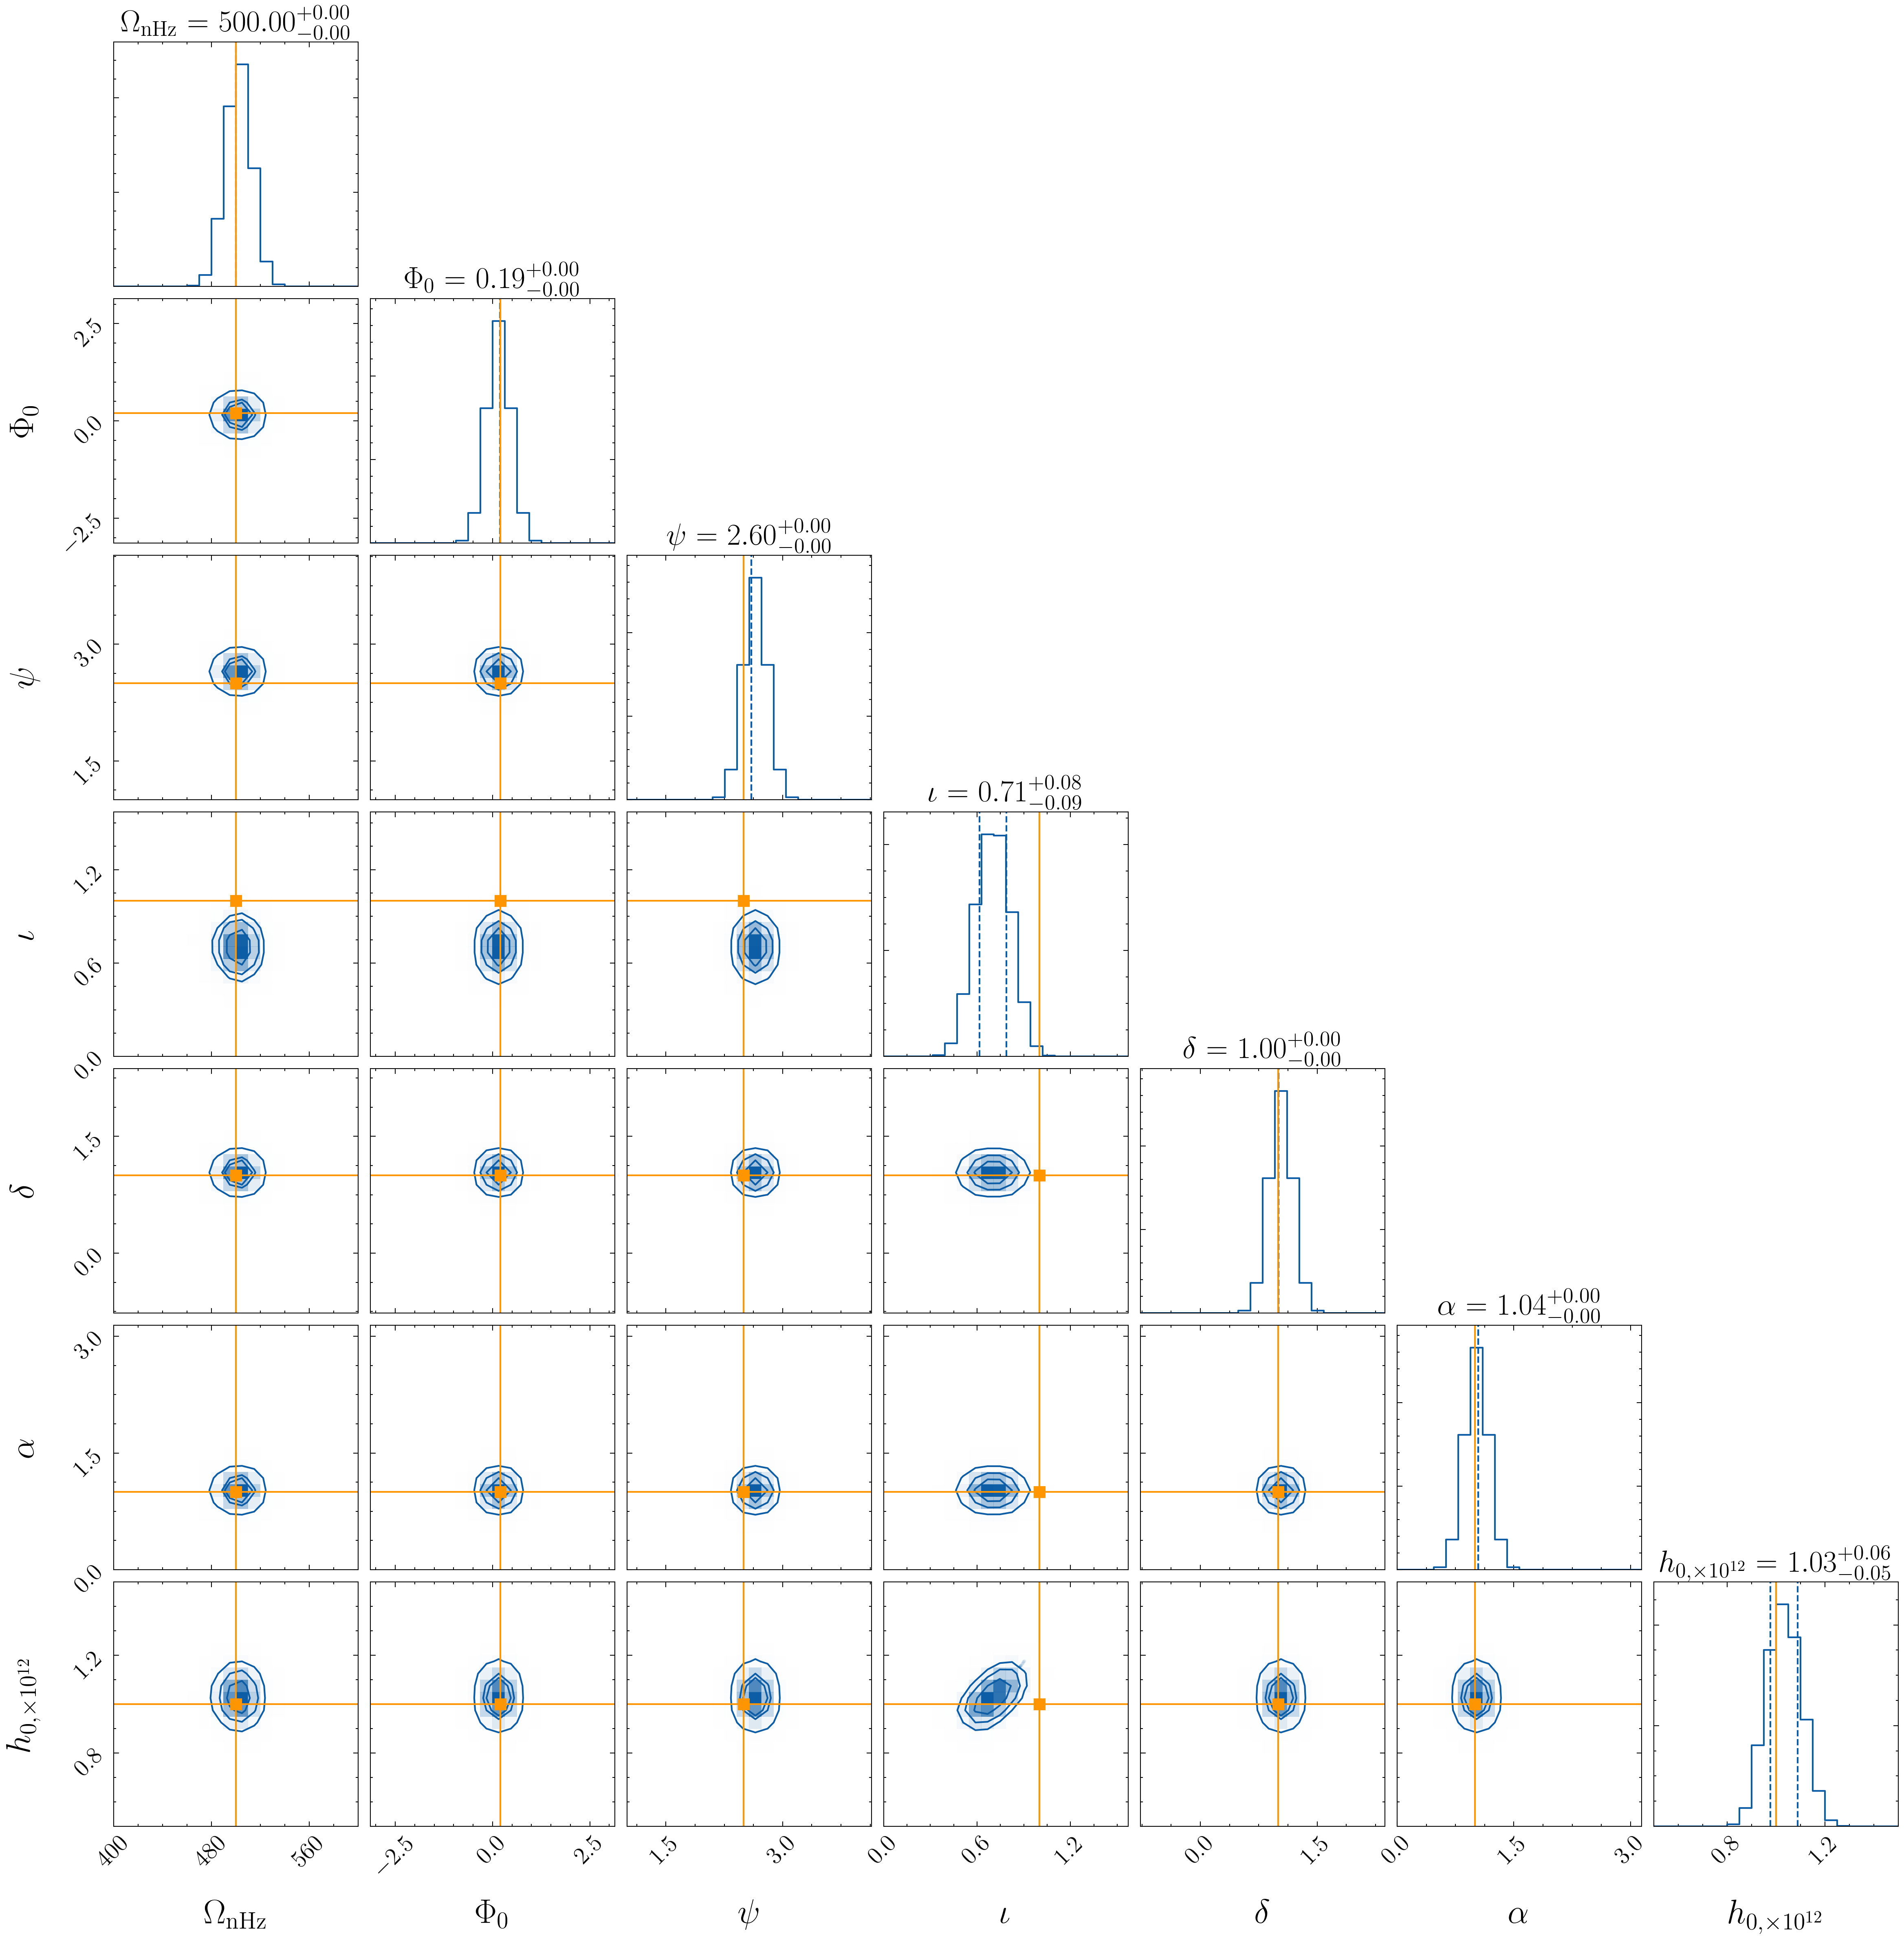
\includegraphics[width=0.8\textwidth, height =0.8\textwidth ]{images/representative_example_v2_GW}
	\caption{Posterior distribution for the GW source parameters $\boldsymbol{\theta}_{\rm gw}$ for a single realisation of the system noise. The vertical orange lines indicate the true injected values, c.f. Table \ref{tab:parameters_and_priors}. The contours in the 2D histograms denote the (0.5, 1, 1.5, 2)-$\sigma$ levels. We are able to accurately estimate each parameter of interest.}
	\label{fig:corner_plot_1}
\end{figure*}

\begin{figure*}%
	\centering
	\subfloat[\centering $f_{\rm em}^{(n)}(t_1)$]{{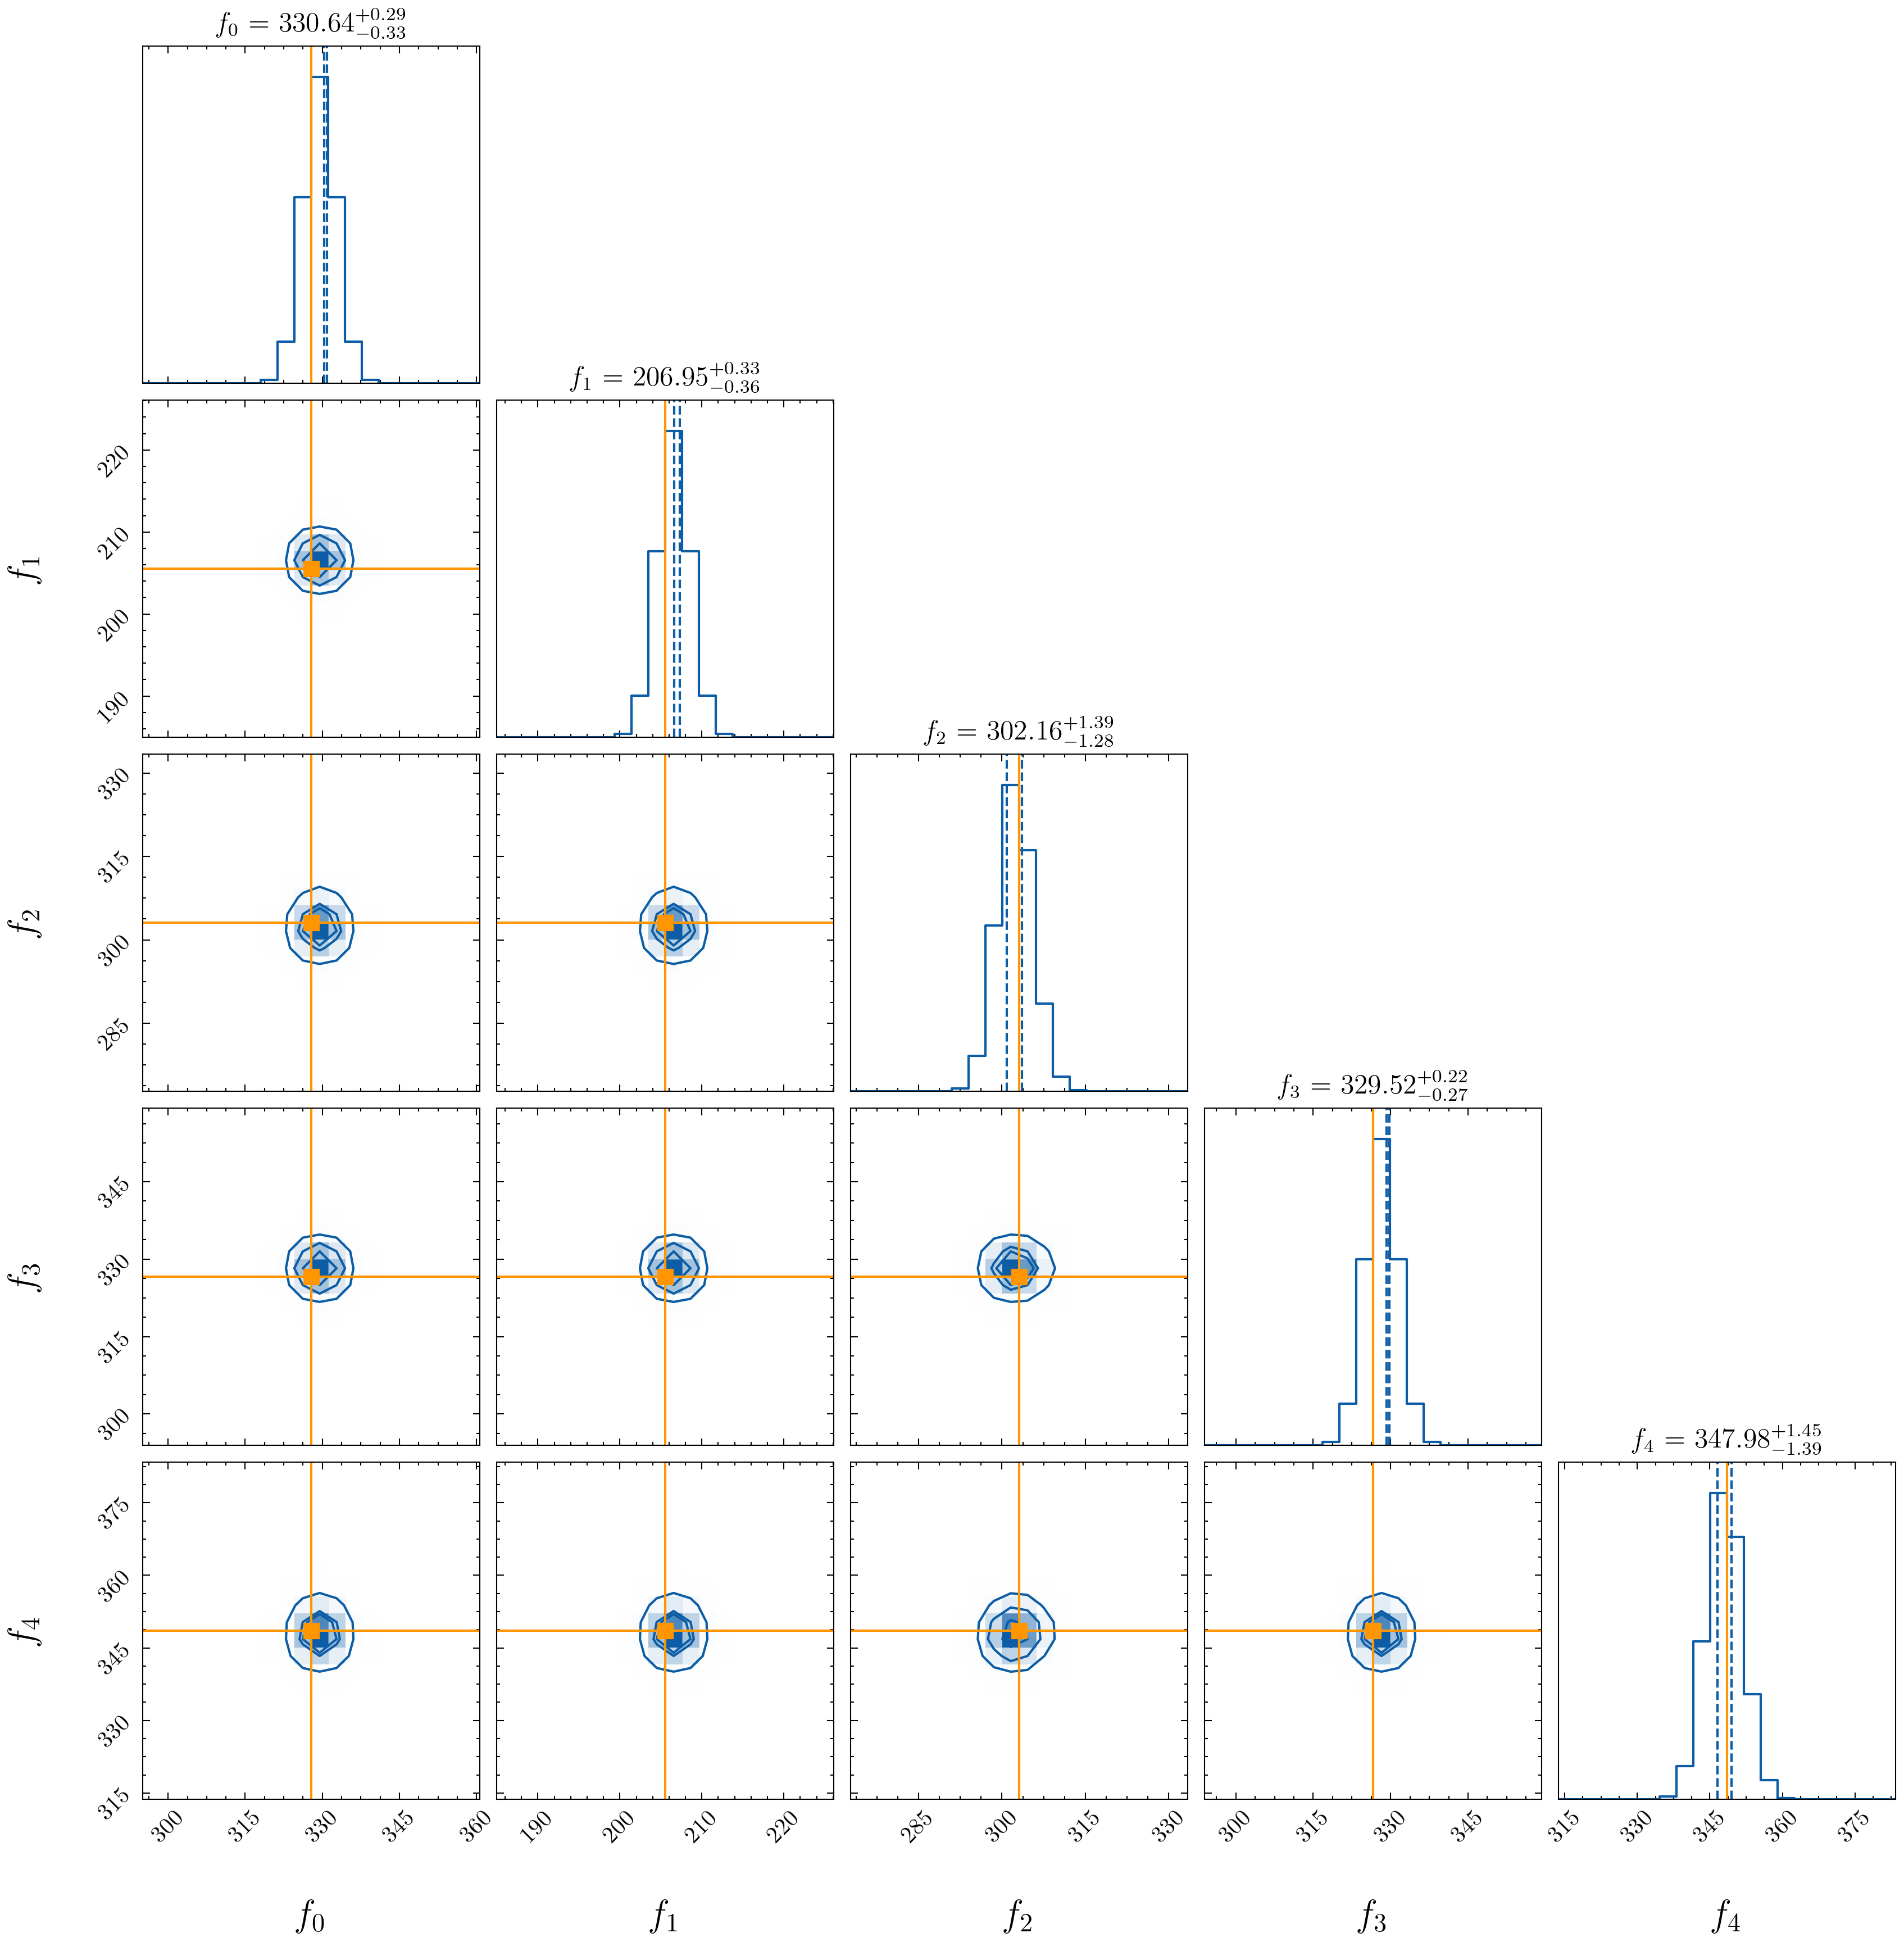
\includegraphics[width=0.3 \textwidth]{images/1237_broad_f} }}%
	\qquad
	\subfloat[\centering $\dot{f}_{\rm em}^{(n)}(t_1)$]{{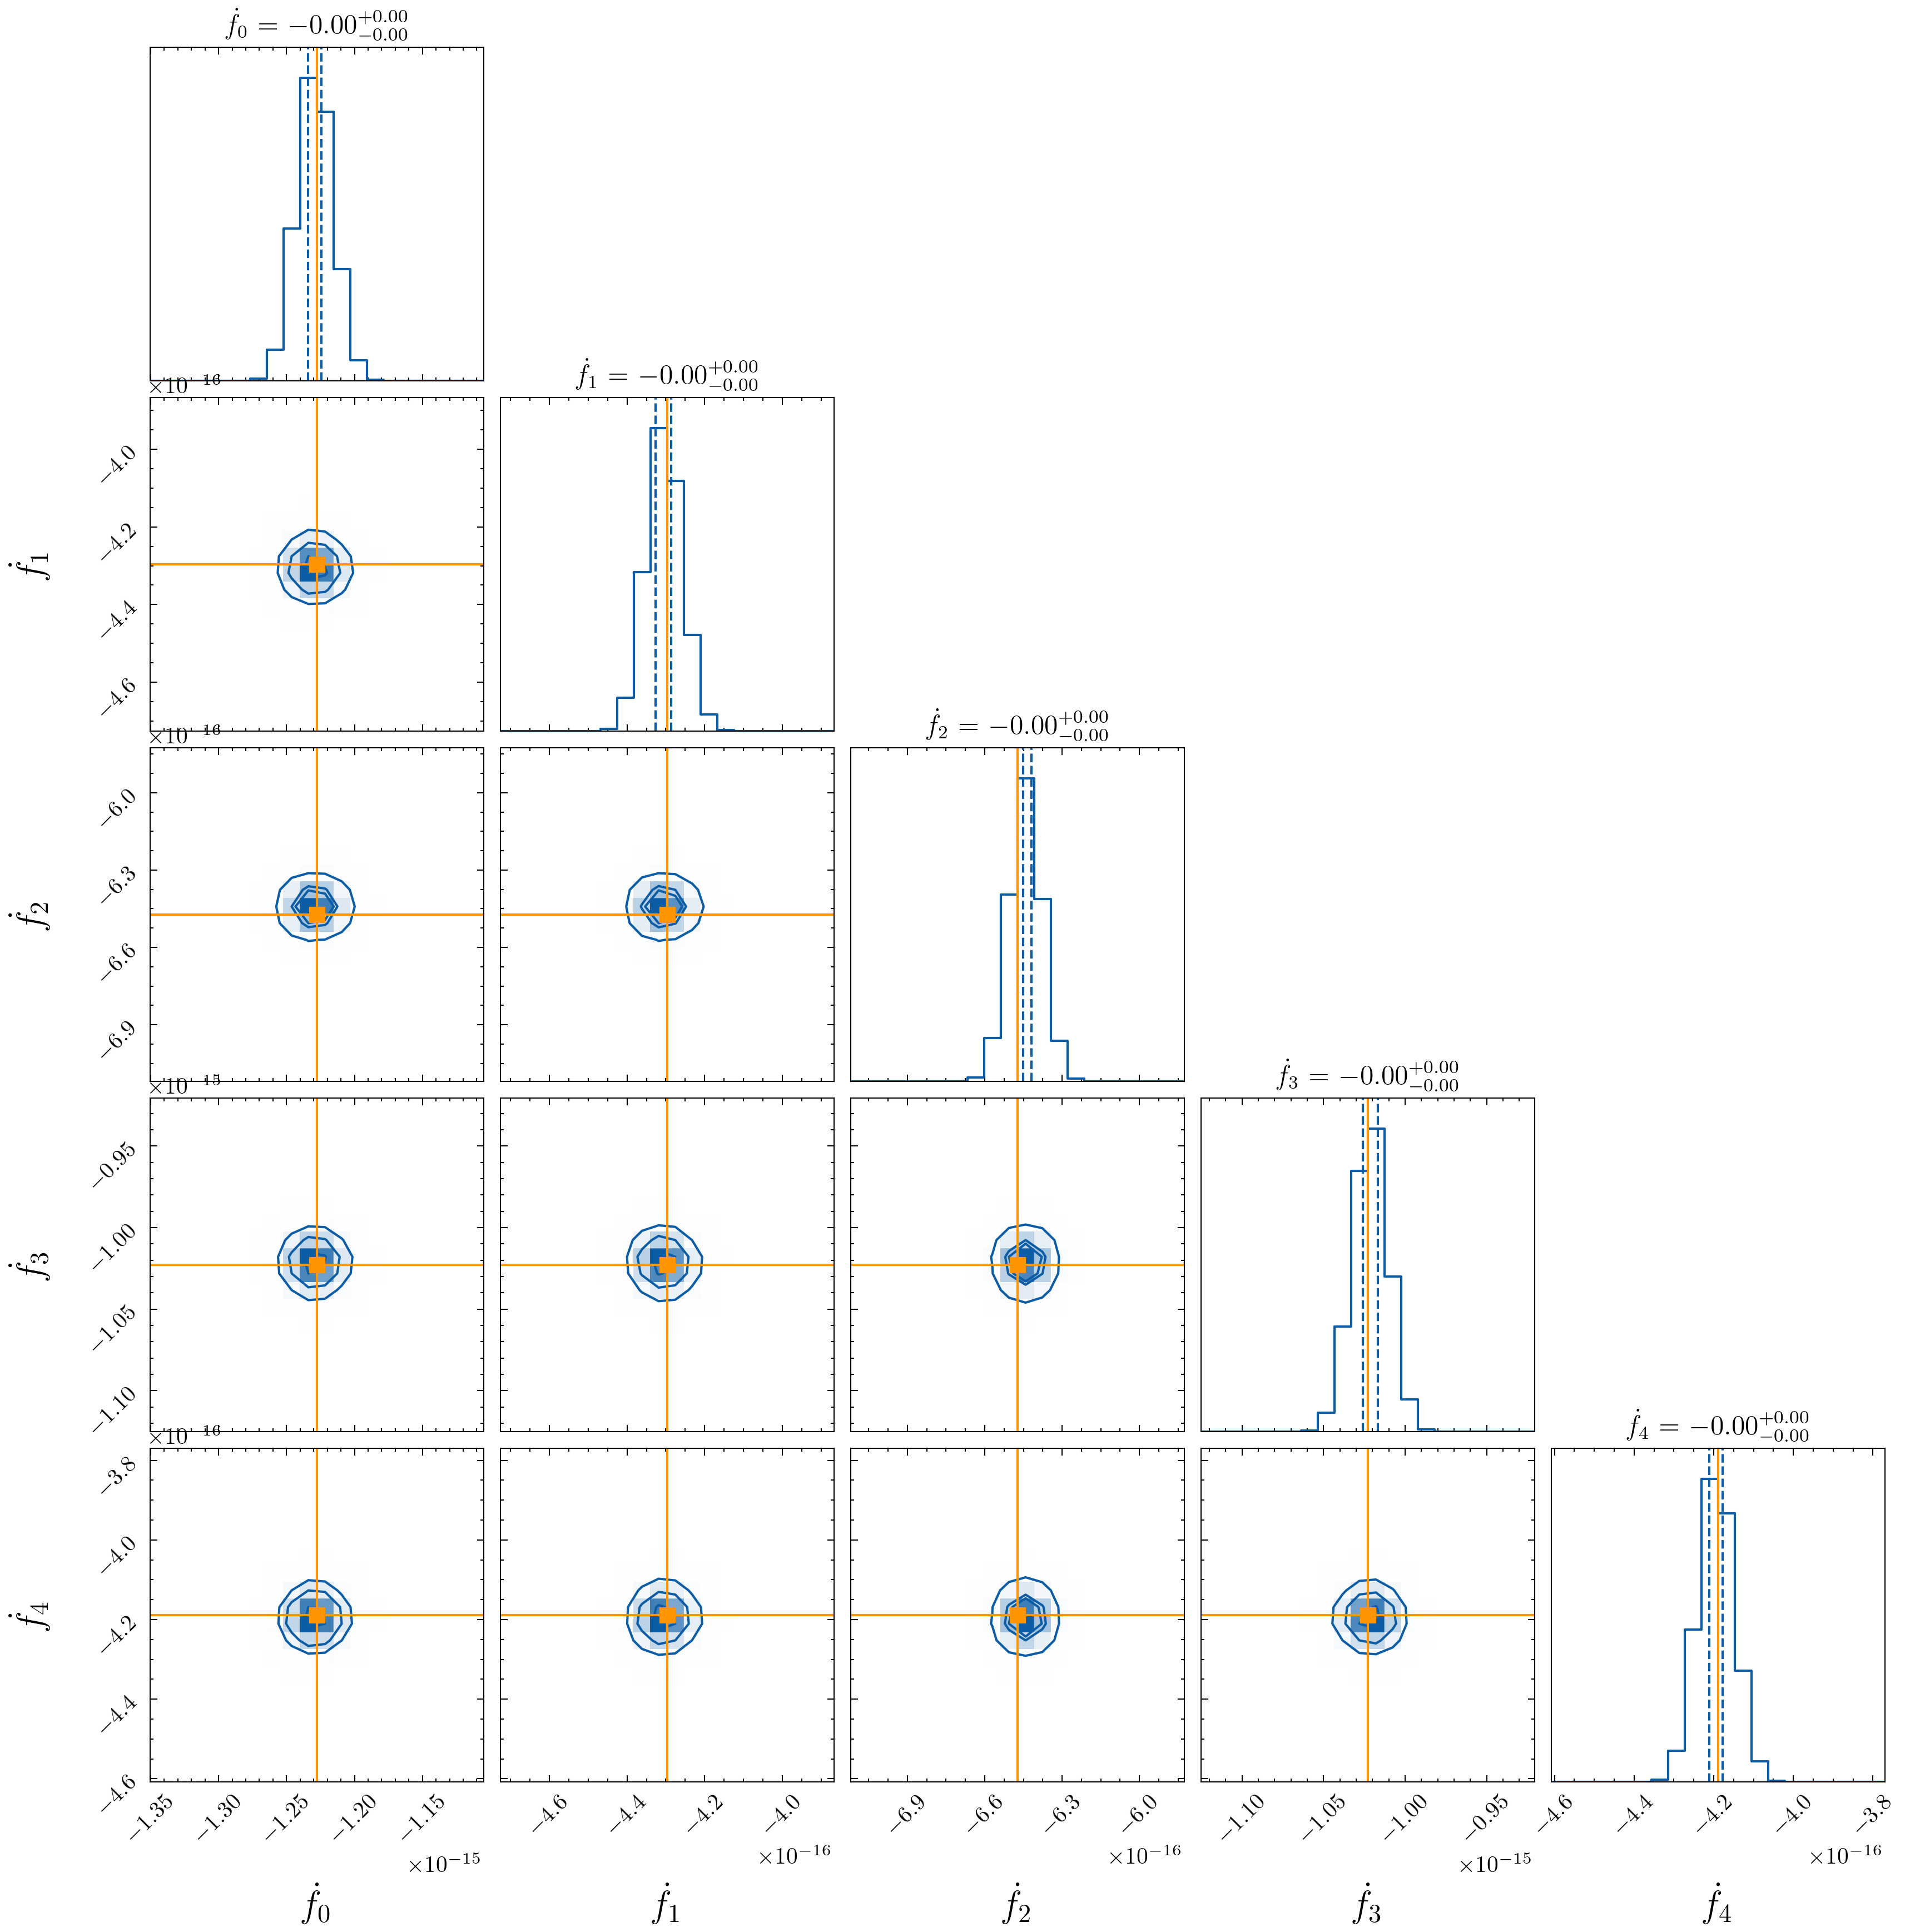
\includegraphics[width=0.3 \textwidth]{images/1237_broad_fdot} }}%
	\qquad
	\subfloat[\centering $\sigma^{(n)}$]{{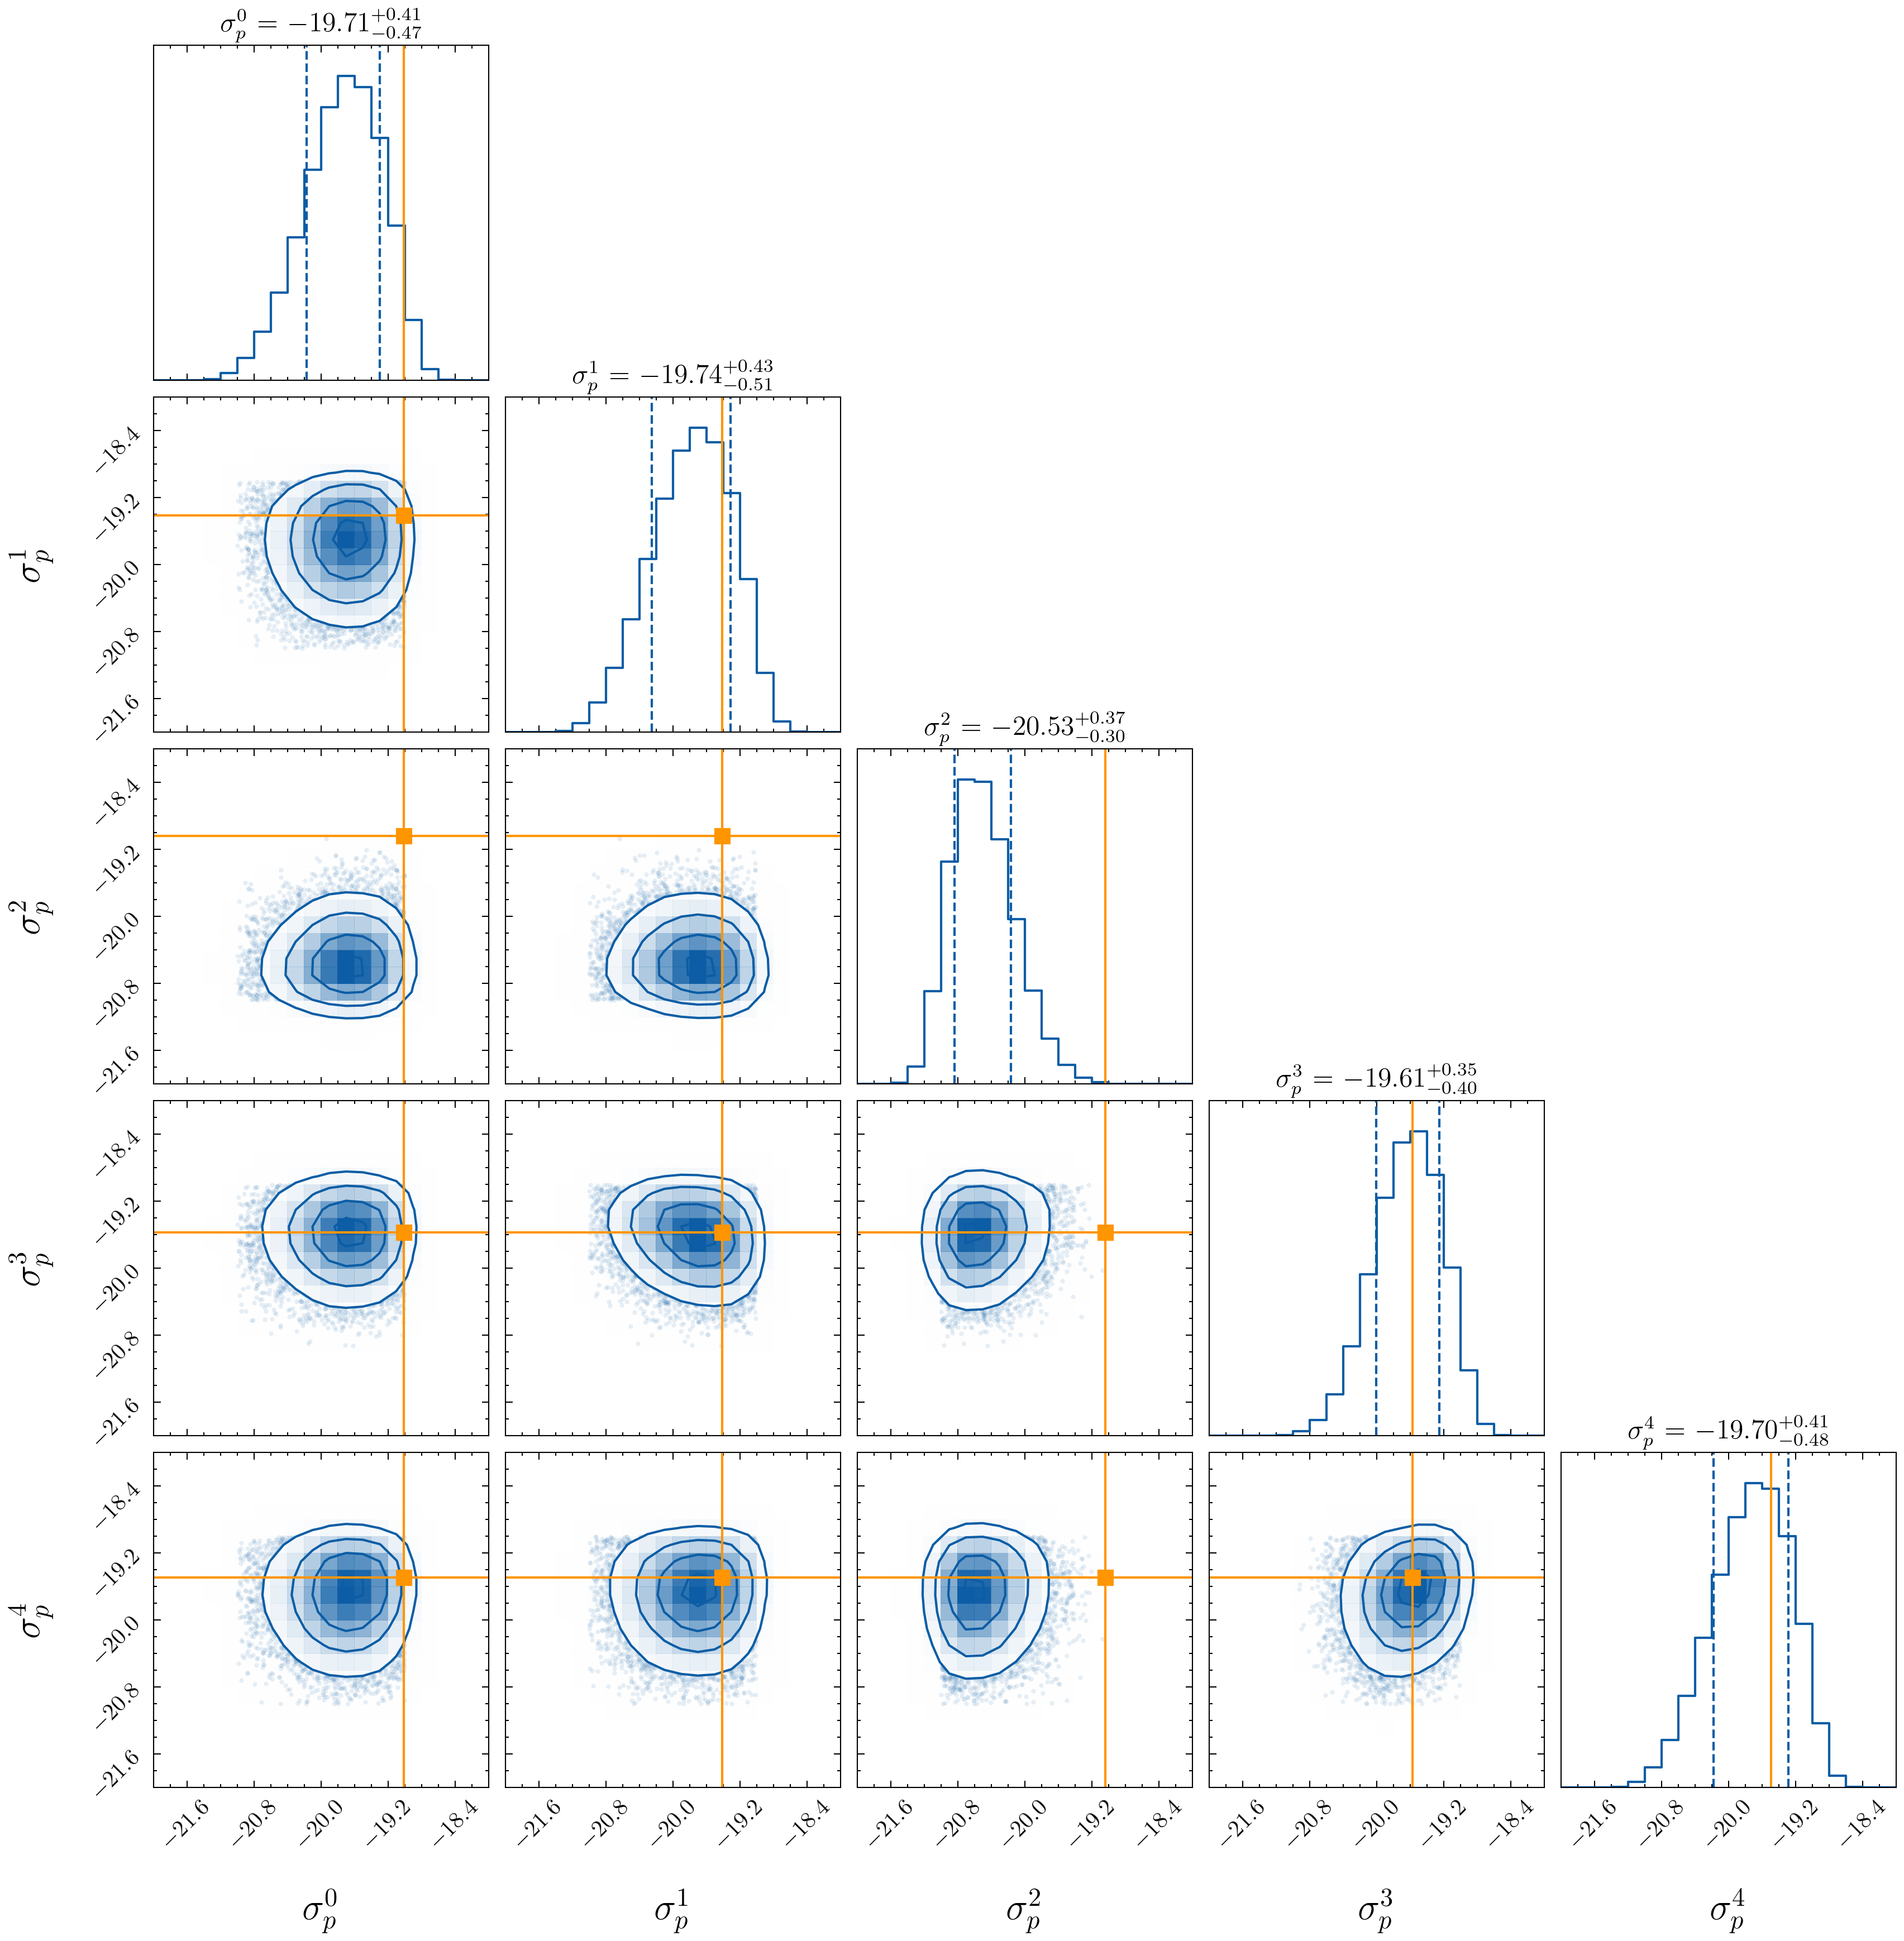
\includegraphics[width=0.3\textwidth]{images/1237_broad_sigma_p} }}%
	
	\caption{As Fig \ref{fig:corner_plot_1} but for the $3N$ pulsar parameters $\boldsymbol{\theta}_{\rm psr, reduced}$. We show only a selection of the first 5 pulsars rather than the full PTA. \textcolor{red}{TK: these figures are a little small to resolve nicely}}
	\label{fig:example_psr_params}%
\end{figure*}








\subsubsection{Detection} \label{sec:detection}
We frame the problem of claiming a detection of a GW in the noisy data in terms of a Bayesian model selection procedure as described in Section \ref{sec:model_selection}. The Bayes factor, $\beta$, as defined in Eq. \ref{eq:bayes} is presented in Fig \ref{fig:bayes} for our representative system, where we now vary the magnitude of the GW strain, $h_0$. The noise processes in the synthetic data are identical realisations for each value of $h_0$; the only change in the data is the change in $h_0$. We can see that there is a general log-linear relationship between $\beta$ and $h_0$ where the GW source is easily detectable with decisive evidence ($\beta \sim 100$) for $h_0 \gtrapprox 10^{-14}$. We take $\beta = 10$ as a tolerance cut-off above which we can accept $\mathcal{M}_1$ and claim a detection of the GW. For this system, given this realisation of the noise, the minimal detectable strain is $\sim 3 \times 10^{-15}$. The small perturbations in the general log-linear $\beta - h_0$ trend arise due to noise in the nested sampling method. For these points the sampler converged sub-optimally for $\mathcal{M}_1$ and so the evidence $\mathcal{Z}(\boldsymbol{Y} | \mathcal{M}_1)$ is lower than would be expected. This is purely a noise artefact; if one recreates the $\beta - h_0$ curve by rerunning the nested sampler these perturbations appear at different values of $h_0$, or else are not present at all. Increasing the number of live points $n_{\rm live}$ used by the nested sampler also dampens these perturbations and smooths the $\beta - h_0$ curve, since as discussed in Section \ref{sec:nested_sampling} the uncertainties in $\mathcal{Z}$ scale as $\mathcal{O}(1/ \sqrt{n_{\rm live}})$. Below $\beta = 10$ this noise in the sampler starts to dominate and the hierarchical relationship between $\mathcal{M}_0$ and  $\mathcal{M}_1$ fails. That is, the requirement that $\mathcal{Z}(\boldsymbol{Y} | \mathcal{M}_1) > \mathcal{Z}(\boldsymbol{Y} | \mathcal{M}_0)$ no longer holds. This is simply due to the fact that at these small strains the system is completely noise dominated and the two models $\mathcal{M}_1, \mathcal{M}_0$ cannot be separated.  \textcolor{red}{TK: Rather than discussing the bumps, maybe just run it again a few times and remove the bumps.}
\begin{figure}
	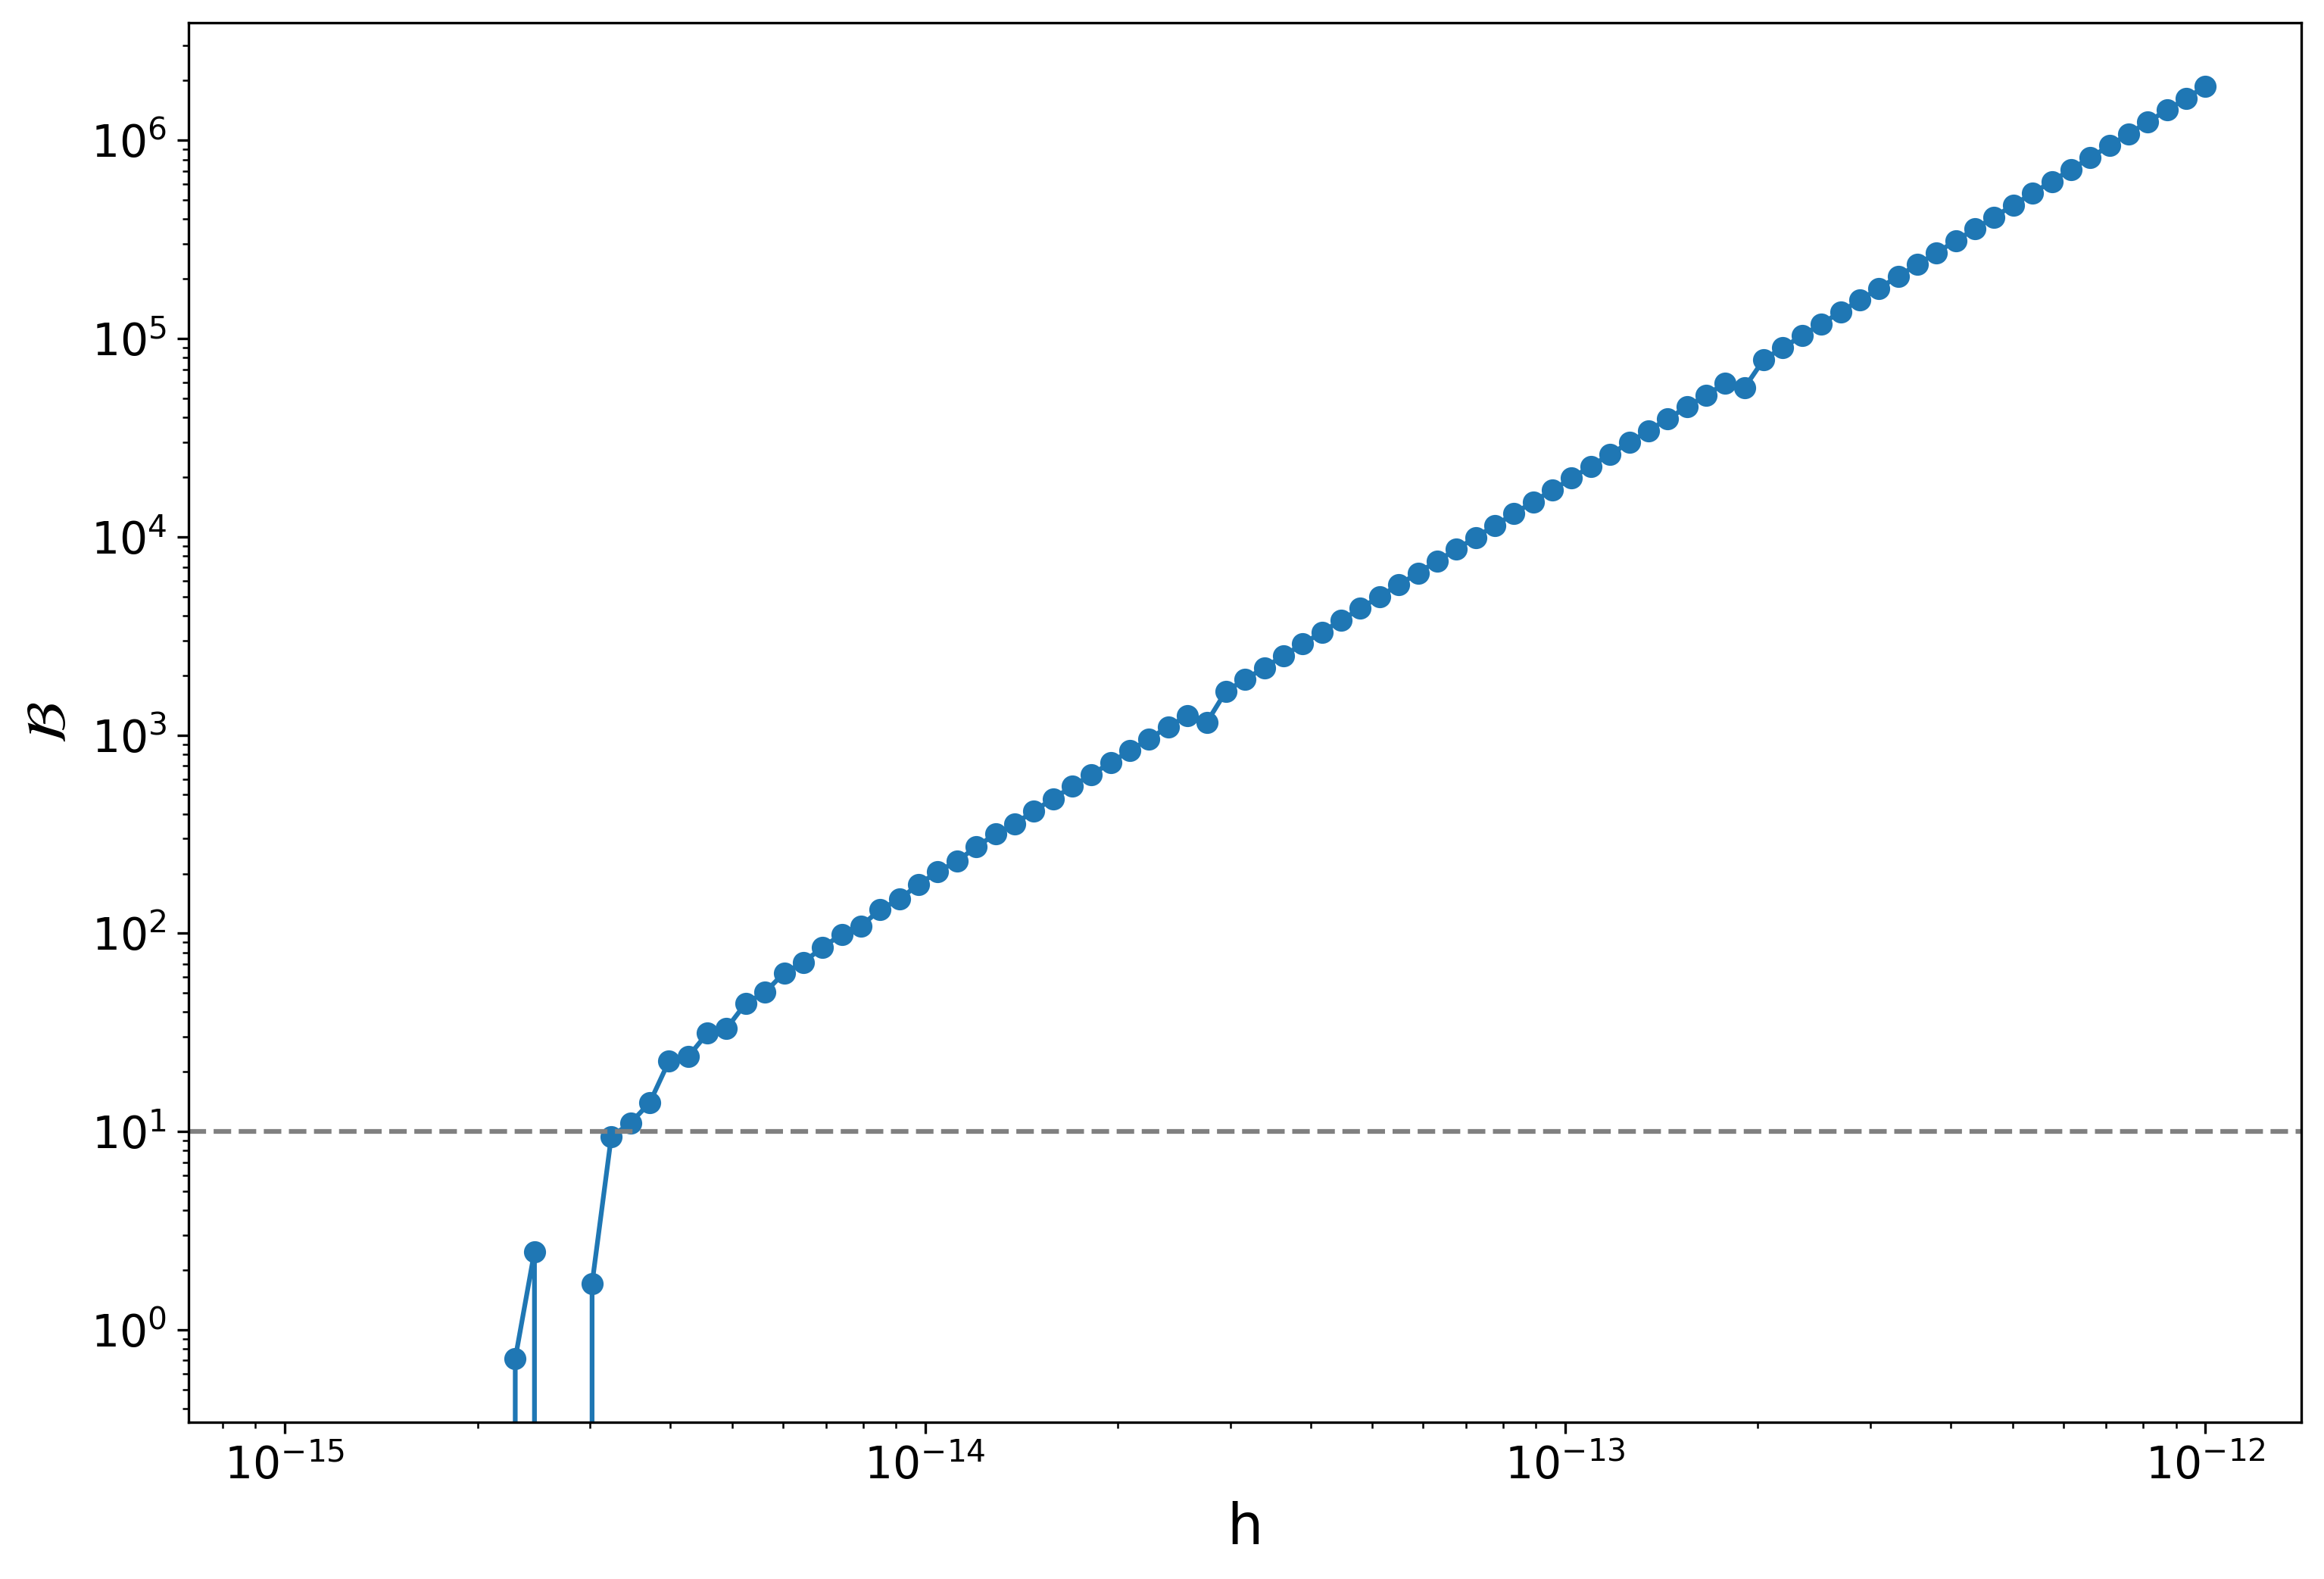
\includegraphics[width=\columnwidth]{images/PaperBayesRatioPlotn1000_stacked}
	\caption{Bayes ratio $\beta$ between the competing models $\mathcal{M}_1$ (GW present in data) and $\mathcal{M}_0$ (GW not present in data) at different GW strain magnitudes $,h_0$, for the representative example summarised in Table \ref{tab:parameters_and_priors}. The horizontal grey dashed line labels the detection tolerance cut-off of $\beta = 10$. The minimal detectable strain, below which $\beta < 10$, is $\sim 3 \times 10^{-15}$. \textcolor{red}{TK: probably need to regenerate this figure to get rid of the "bumps" which are just artefacts from a poor sampler convergence at that point}}
	\label{fig:bayes}
\end{figure}

\subsubsection{Multiple noise realisations} \label{sec:multiple_noise}
\begin{figure*}
	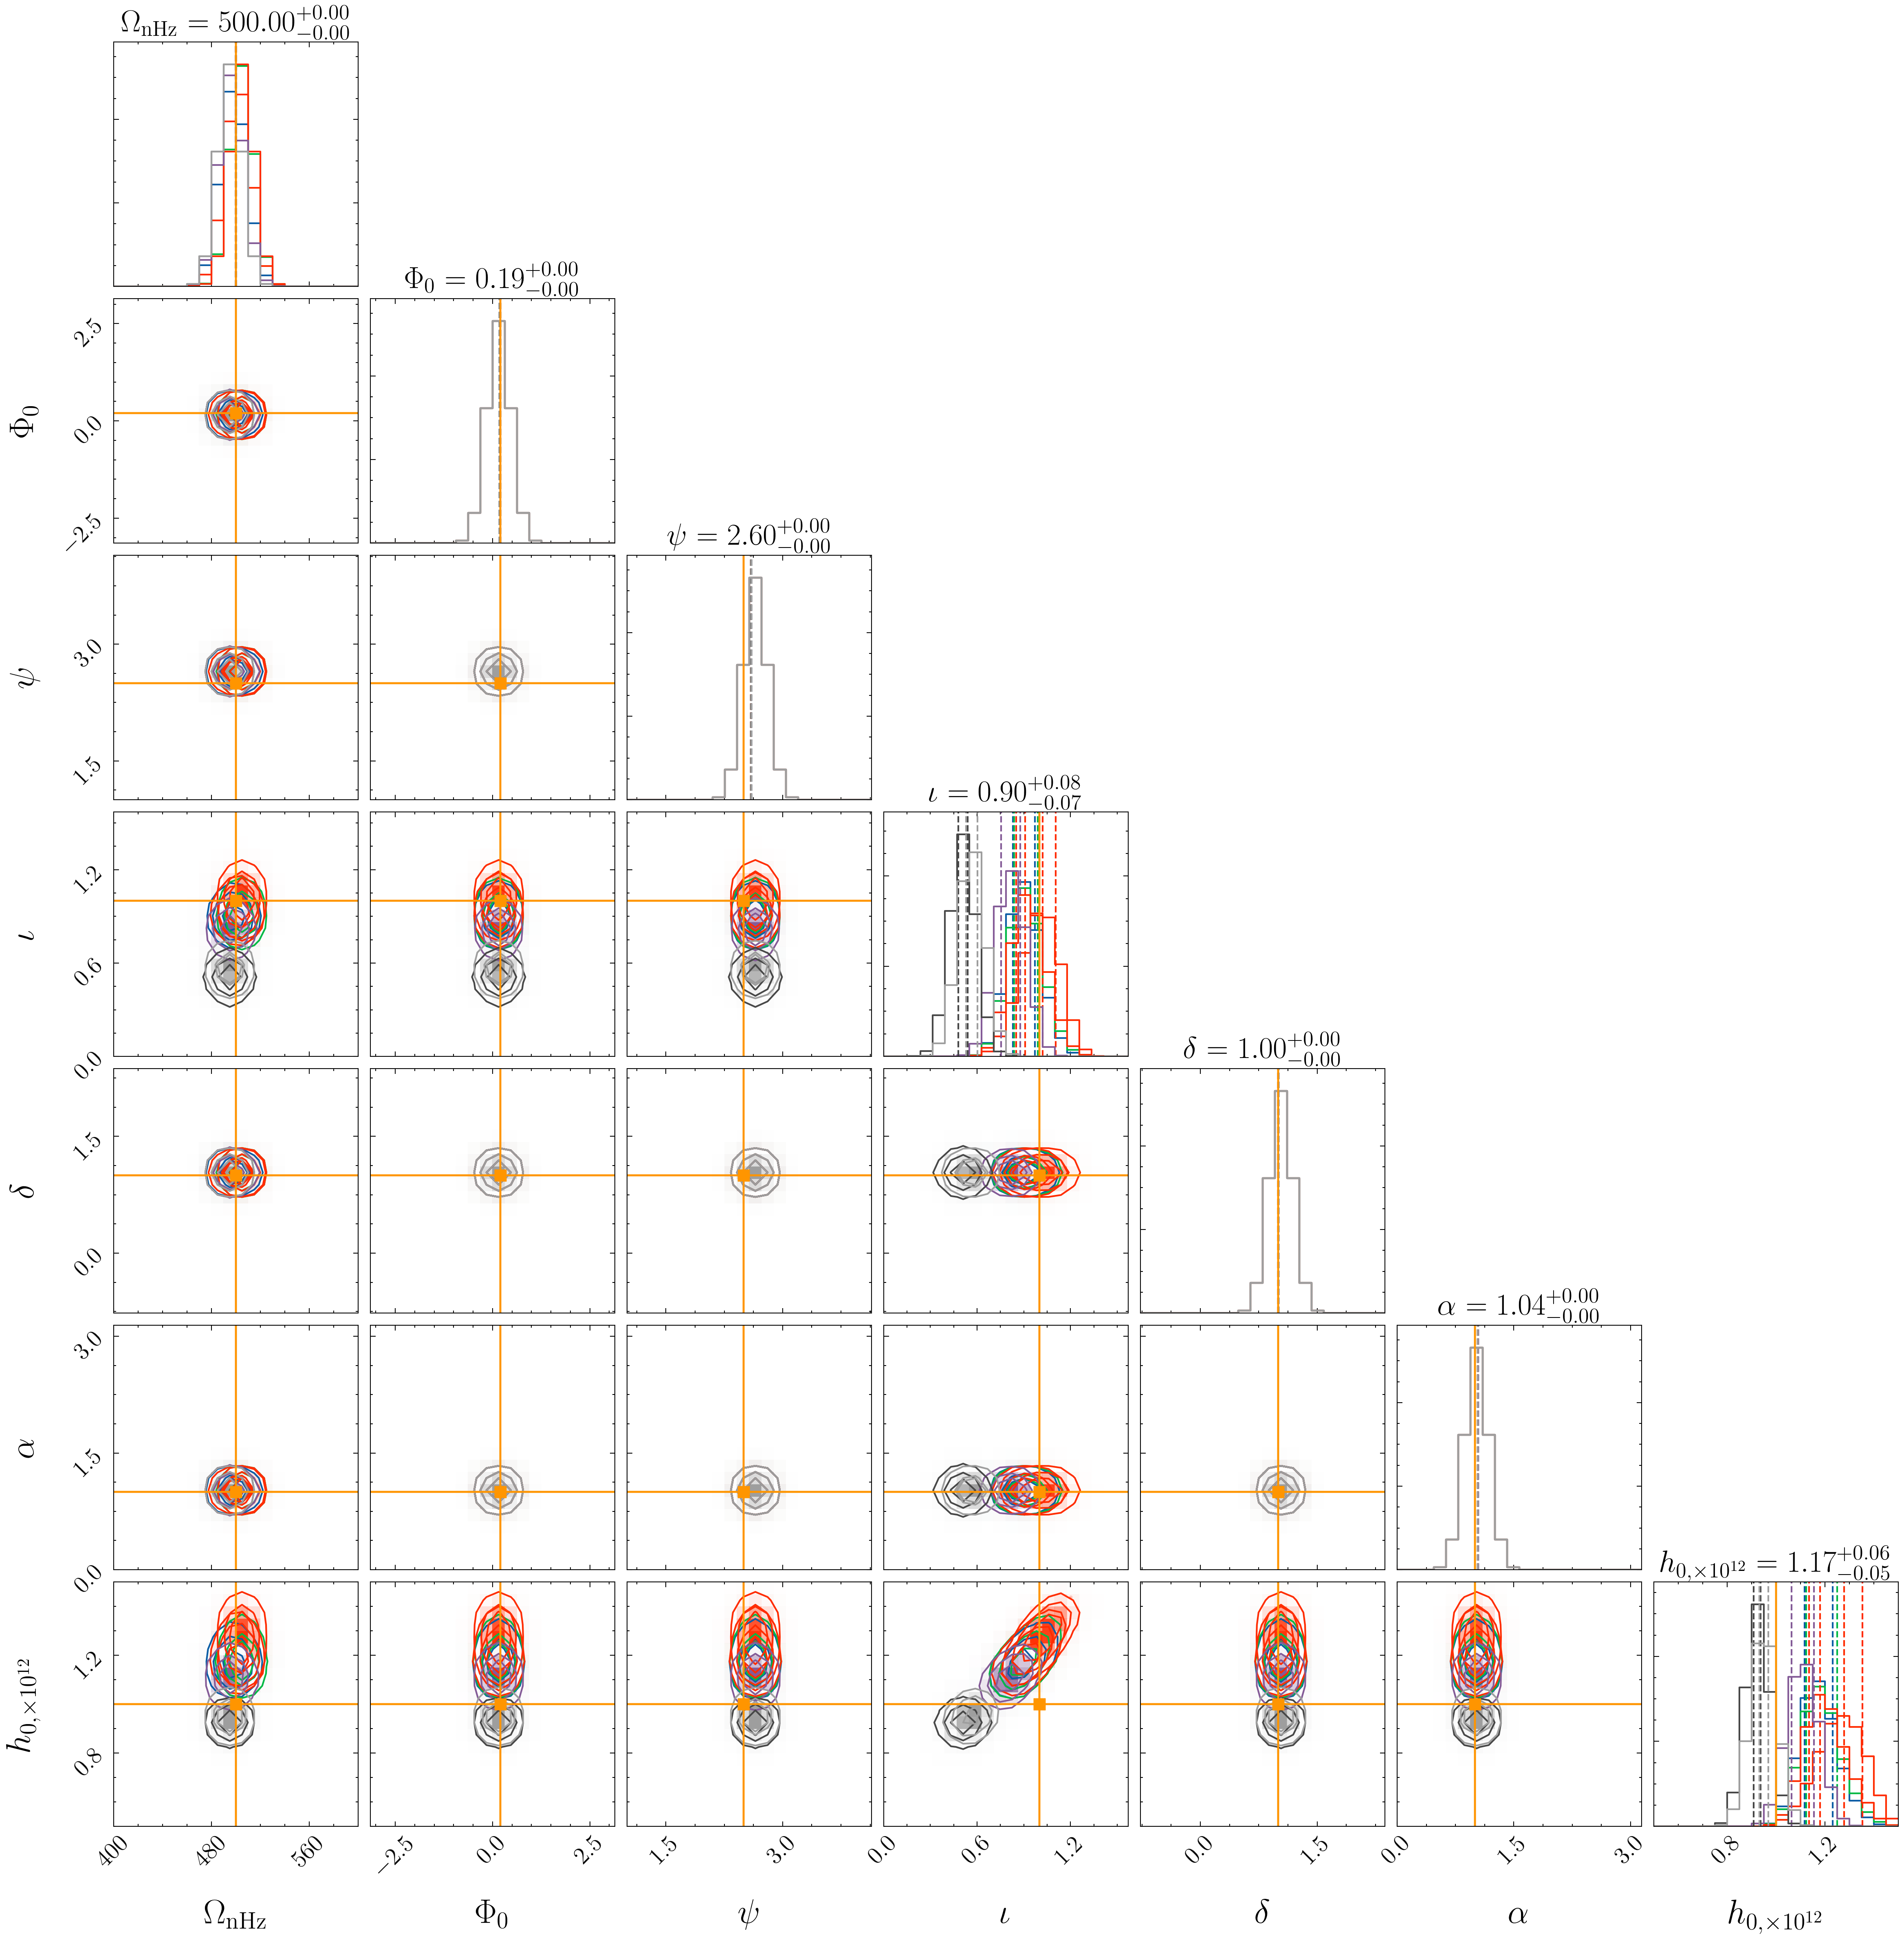
\includegraphics[width=0.8\textwidth, height =0.8\textwidth ]{images/stacked_GW_plot_1000}
	\caption{As Figure \ref{fig:corner_plot_1} but for 9 realisations of the noise processes. The inferred posterior distributions show strong agreement between the different noise realisations for the majority of static parameters. The exceptions are $\iota$ and $h$ which exhibit a larger degree of variance.} 
	\label{fig:corner_plot_2}
\end{figure*}
\begin{figure*}
	\centering
	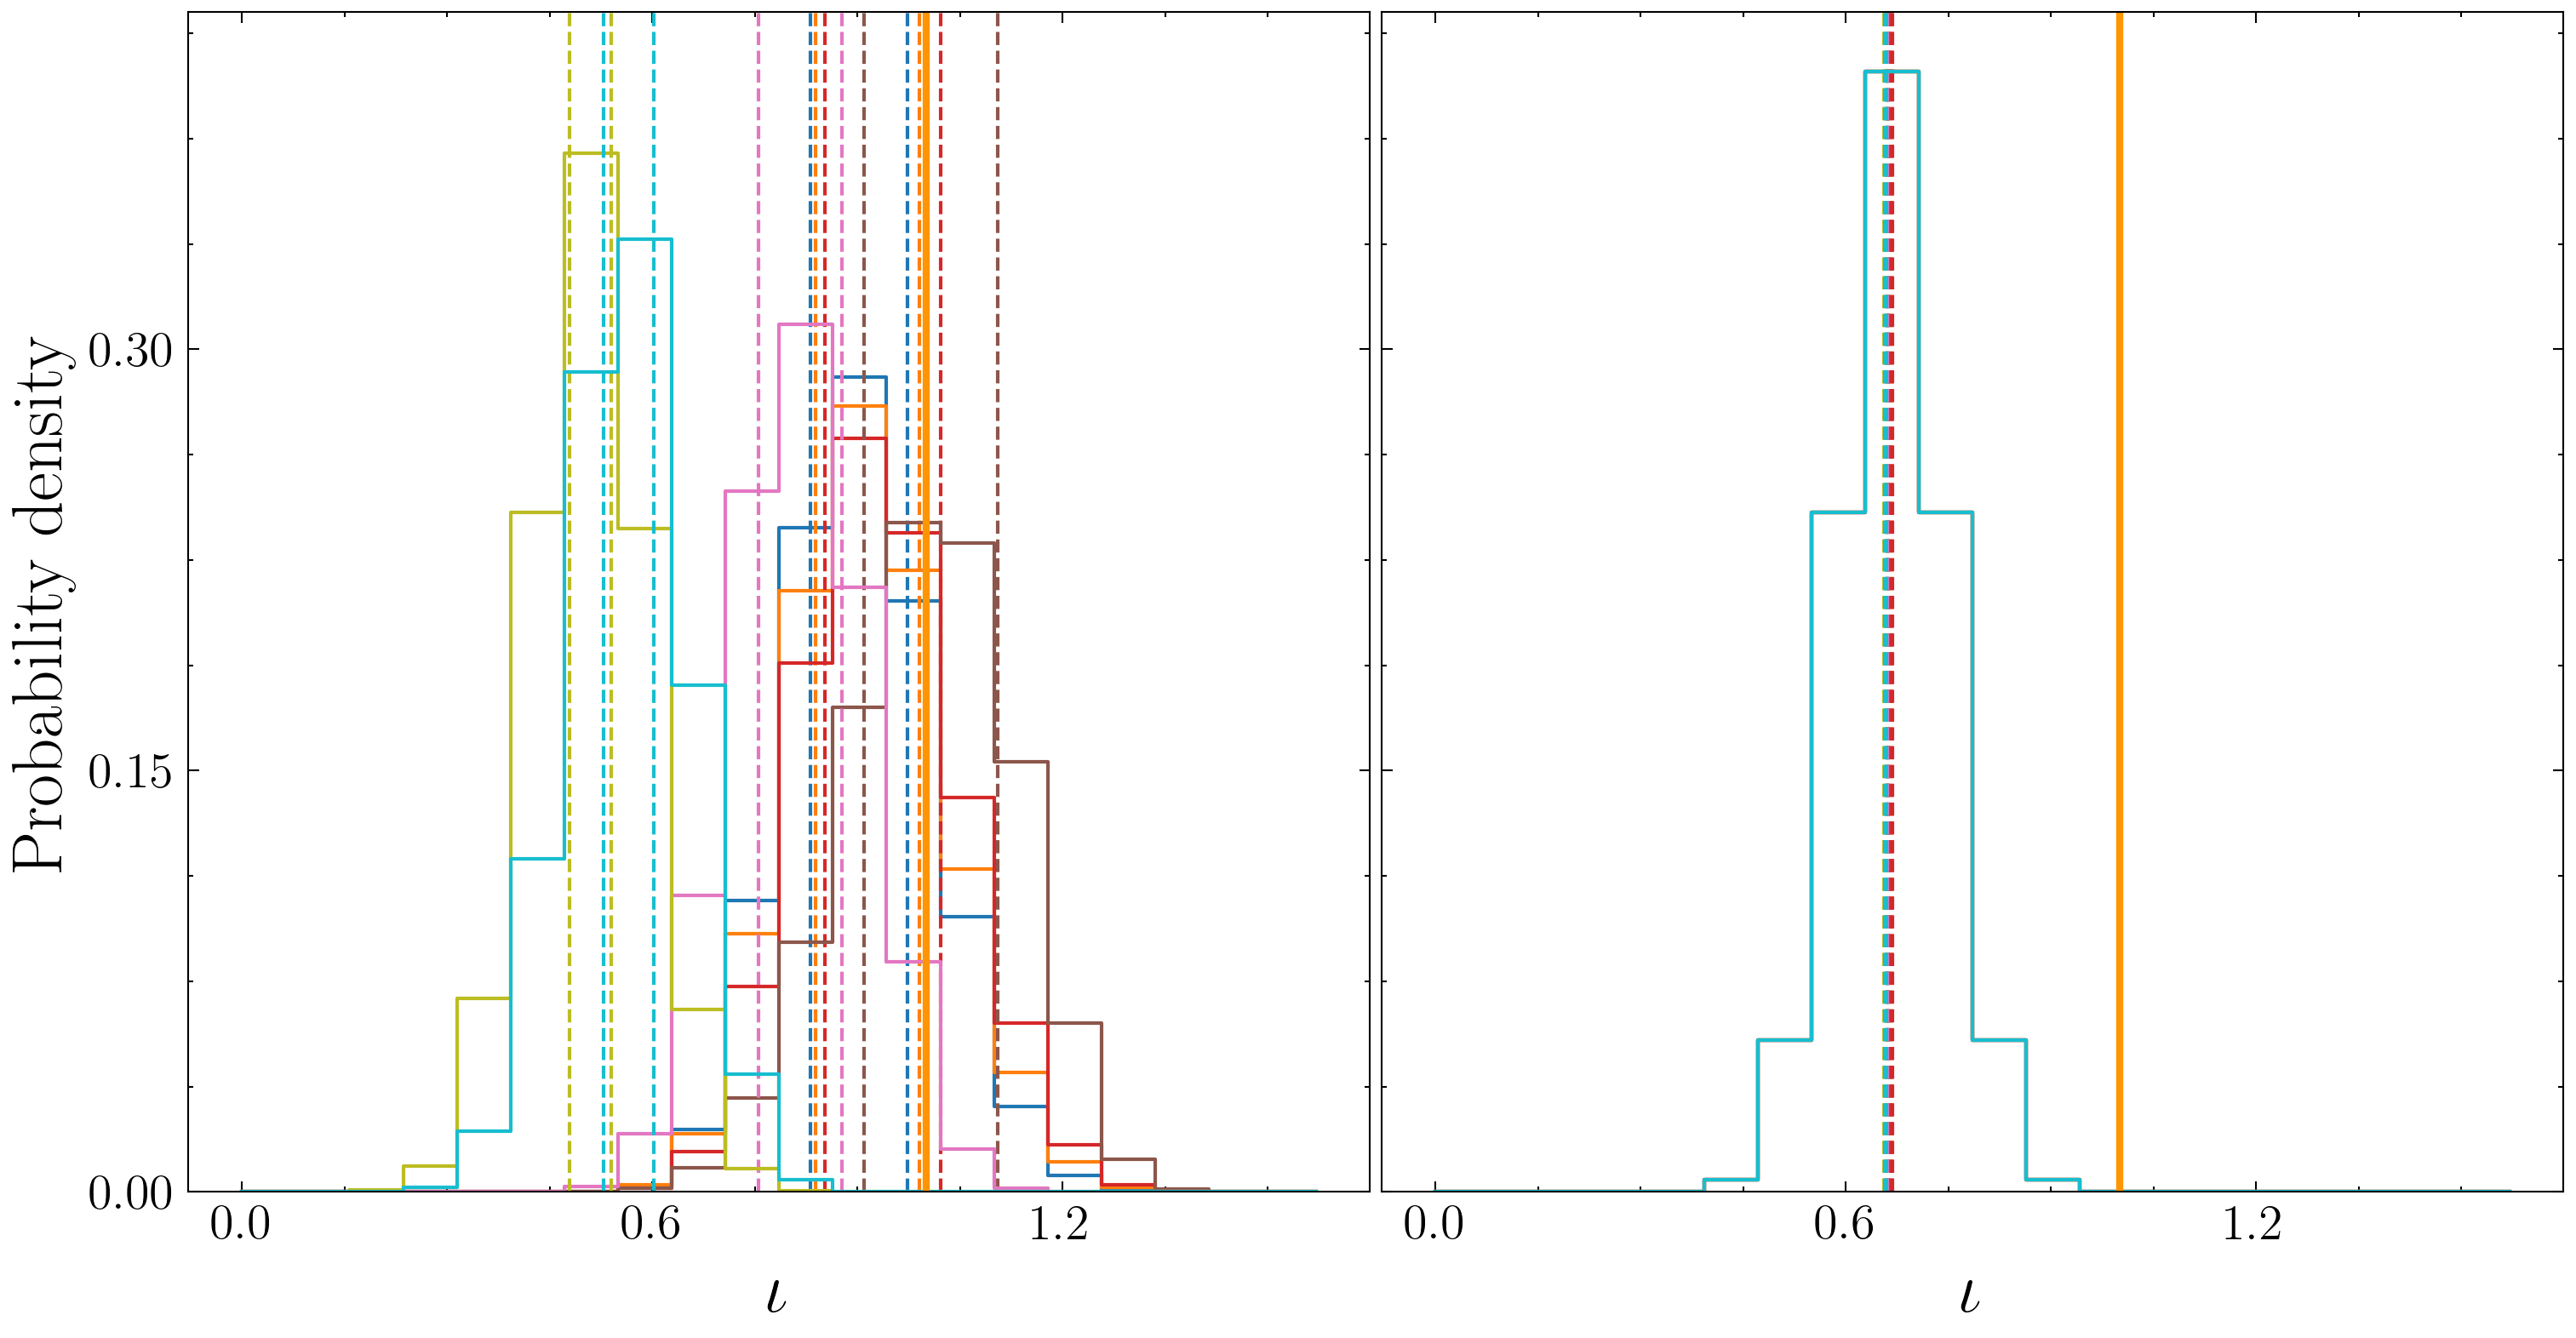
\includegraphics[width=\textwidth]{images/compare_iotas_lines2}
	\caption{1D marginalized posteriors for $\iota$ over 9 realisations of the noise where $h$ is (a) an unknown free parameter (left panel) and (b) fixed at its true value $= 10^{-12}$. The left hand panel is equivalent to the marginalized posteriors for $\iota$ shown in Figure \ref{fig:corner_plot_2} (4th row, 4th column). The thick orange line labels the true injected value. Fixing $h$ reduces the variance between different noise realisations but results in a clear bias between the true and inferred values of $\iota$.}
	\label{fig:iota}
\end{figure*}
\begin{figure*}
	\setkeys{Gin}{width=\linewidth}   
	
	\begin{subfigure}[b]{0.3\textwidth}
		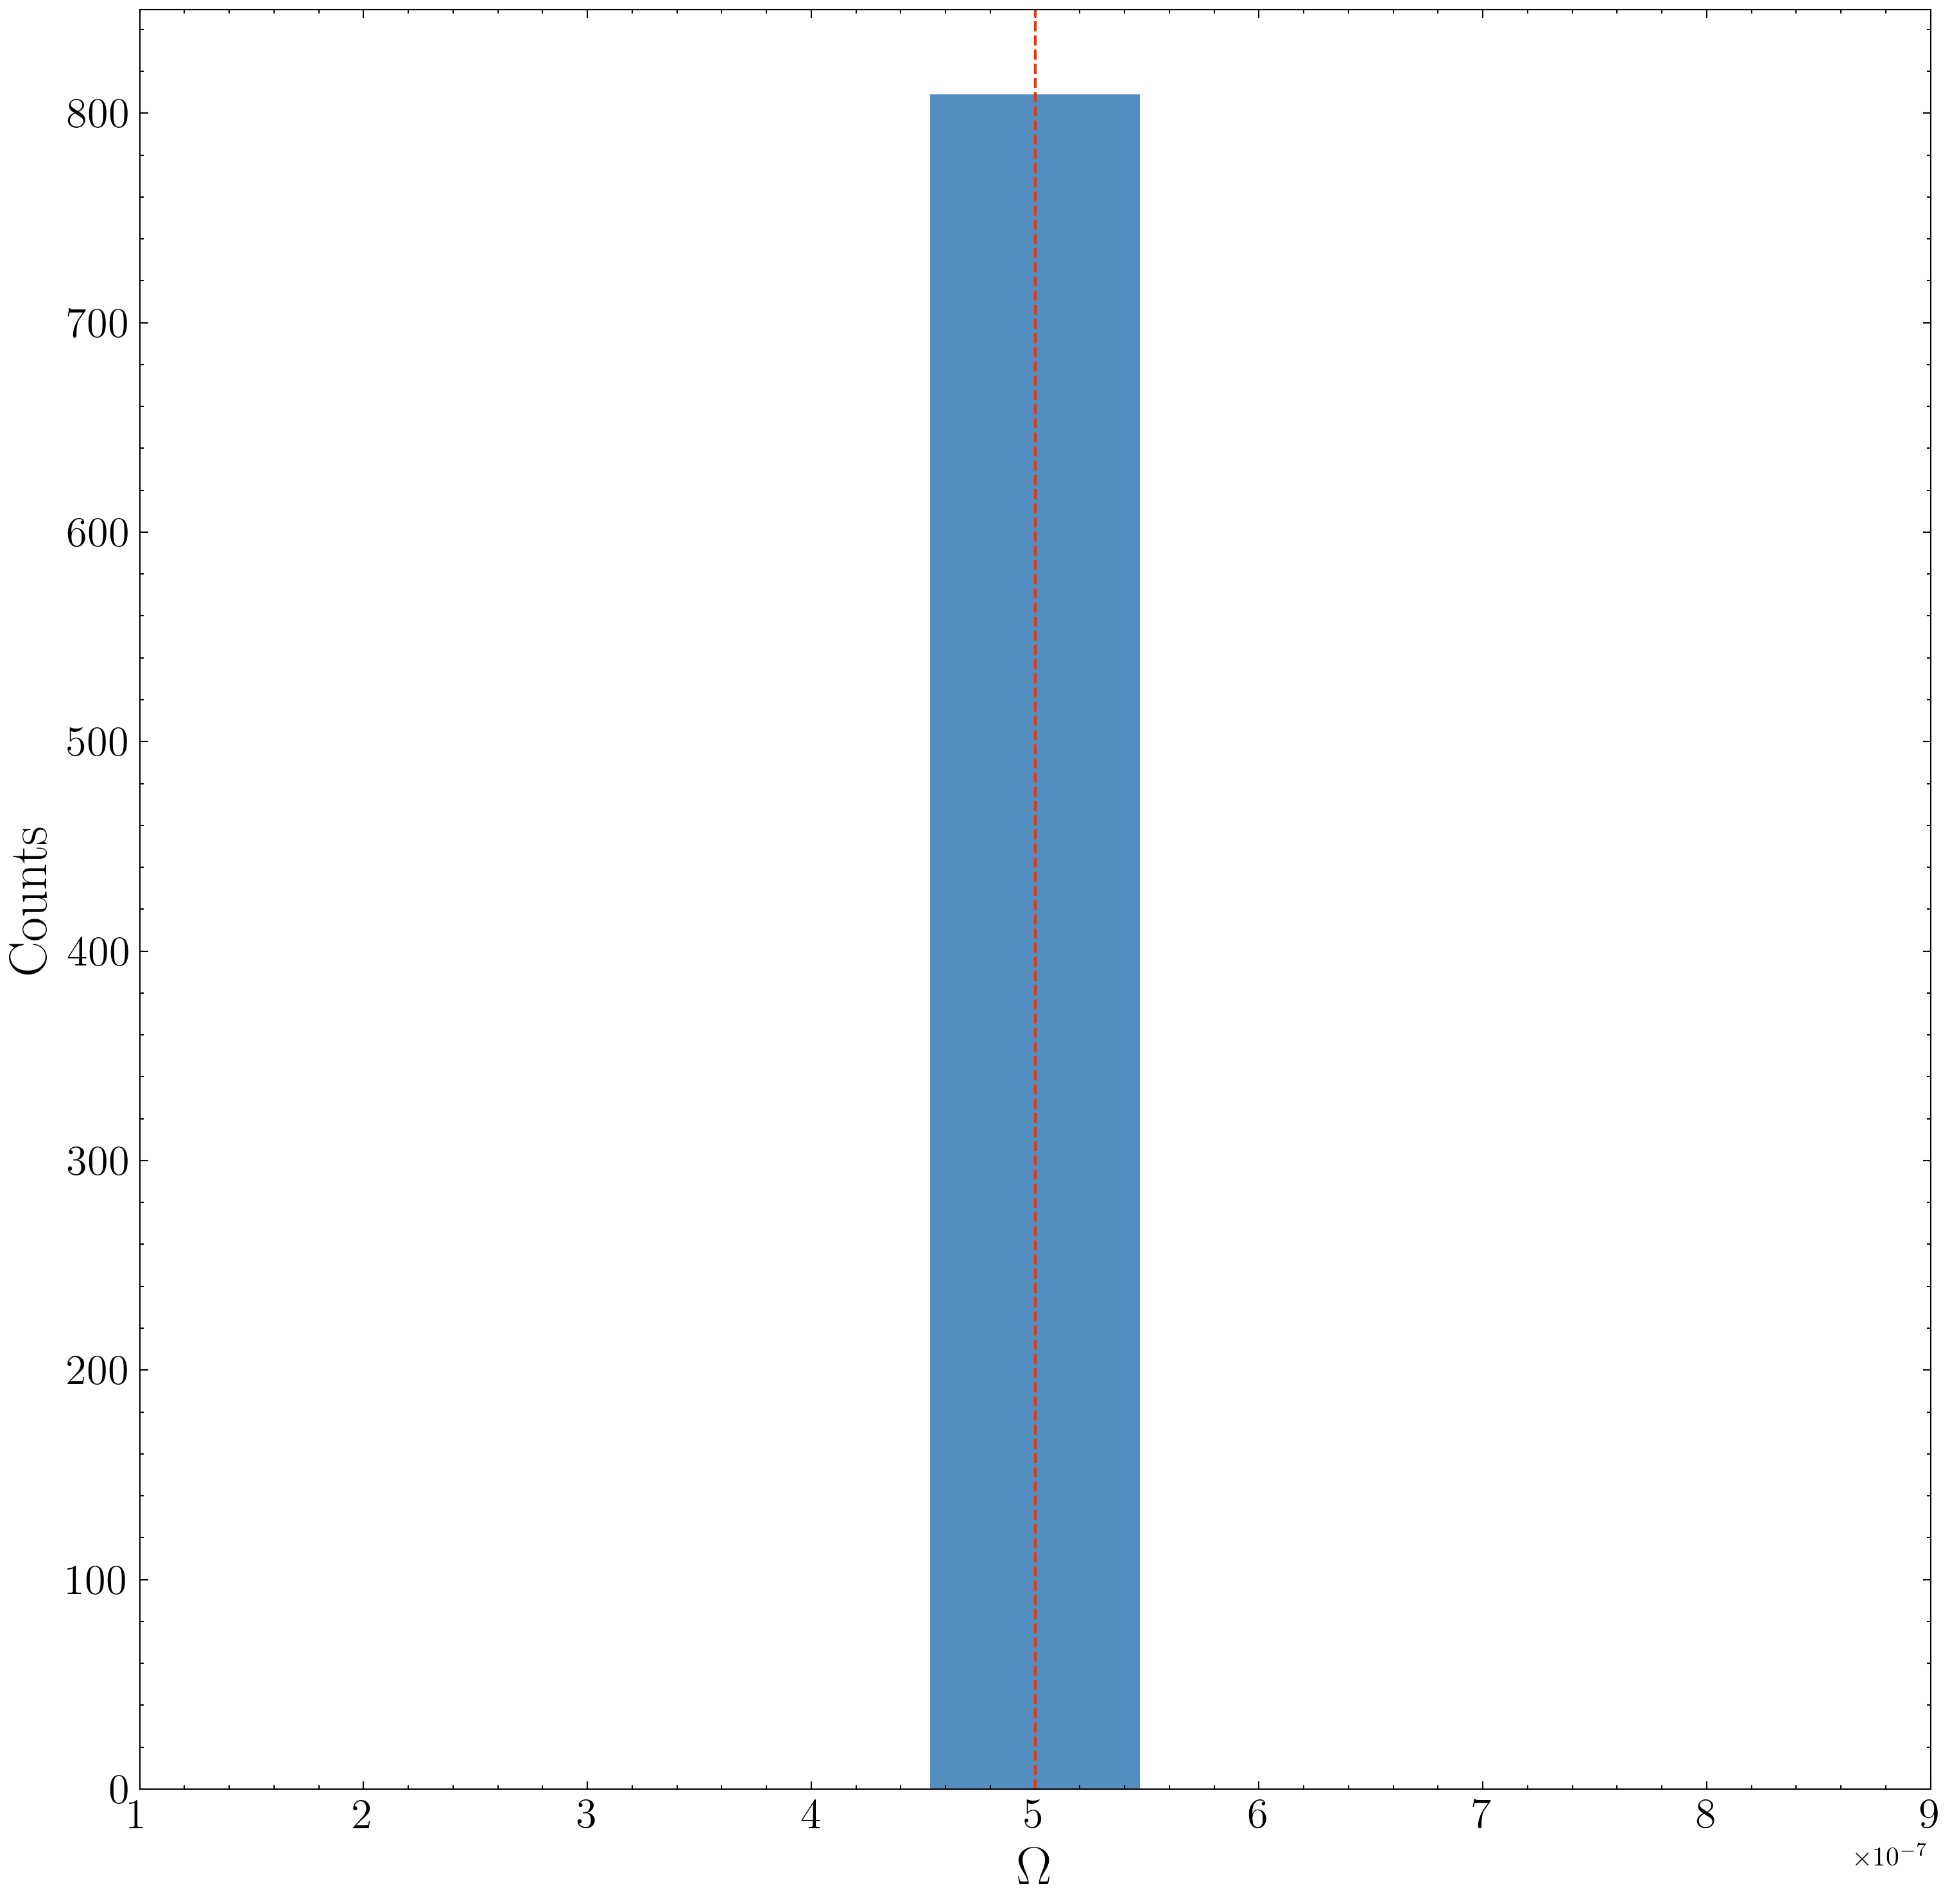
\includegraphics[width=\textwidth]{images/distribution_omega_gw}
		\caption{$\Omega$}
	\end{subfigure}
	\hfill
	\begin{subfigure}[b]{0.3\textwidth}
		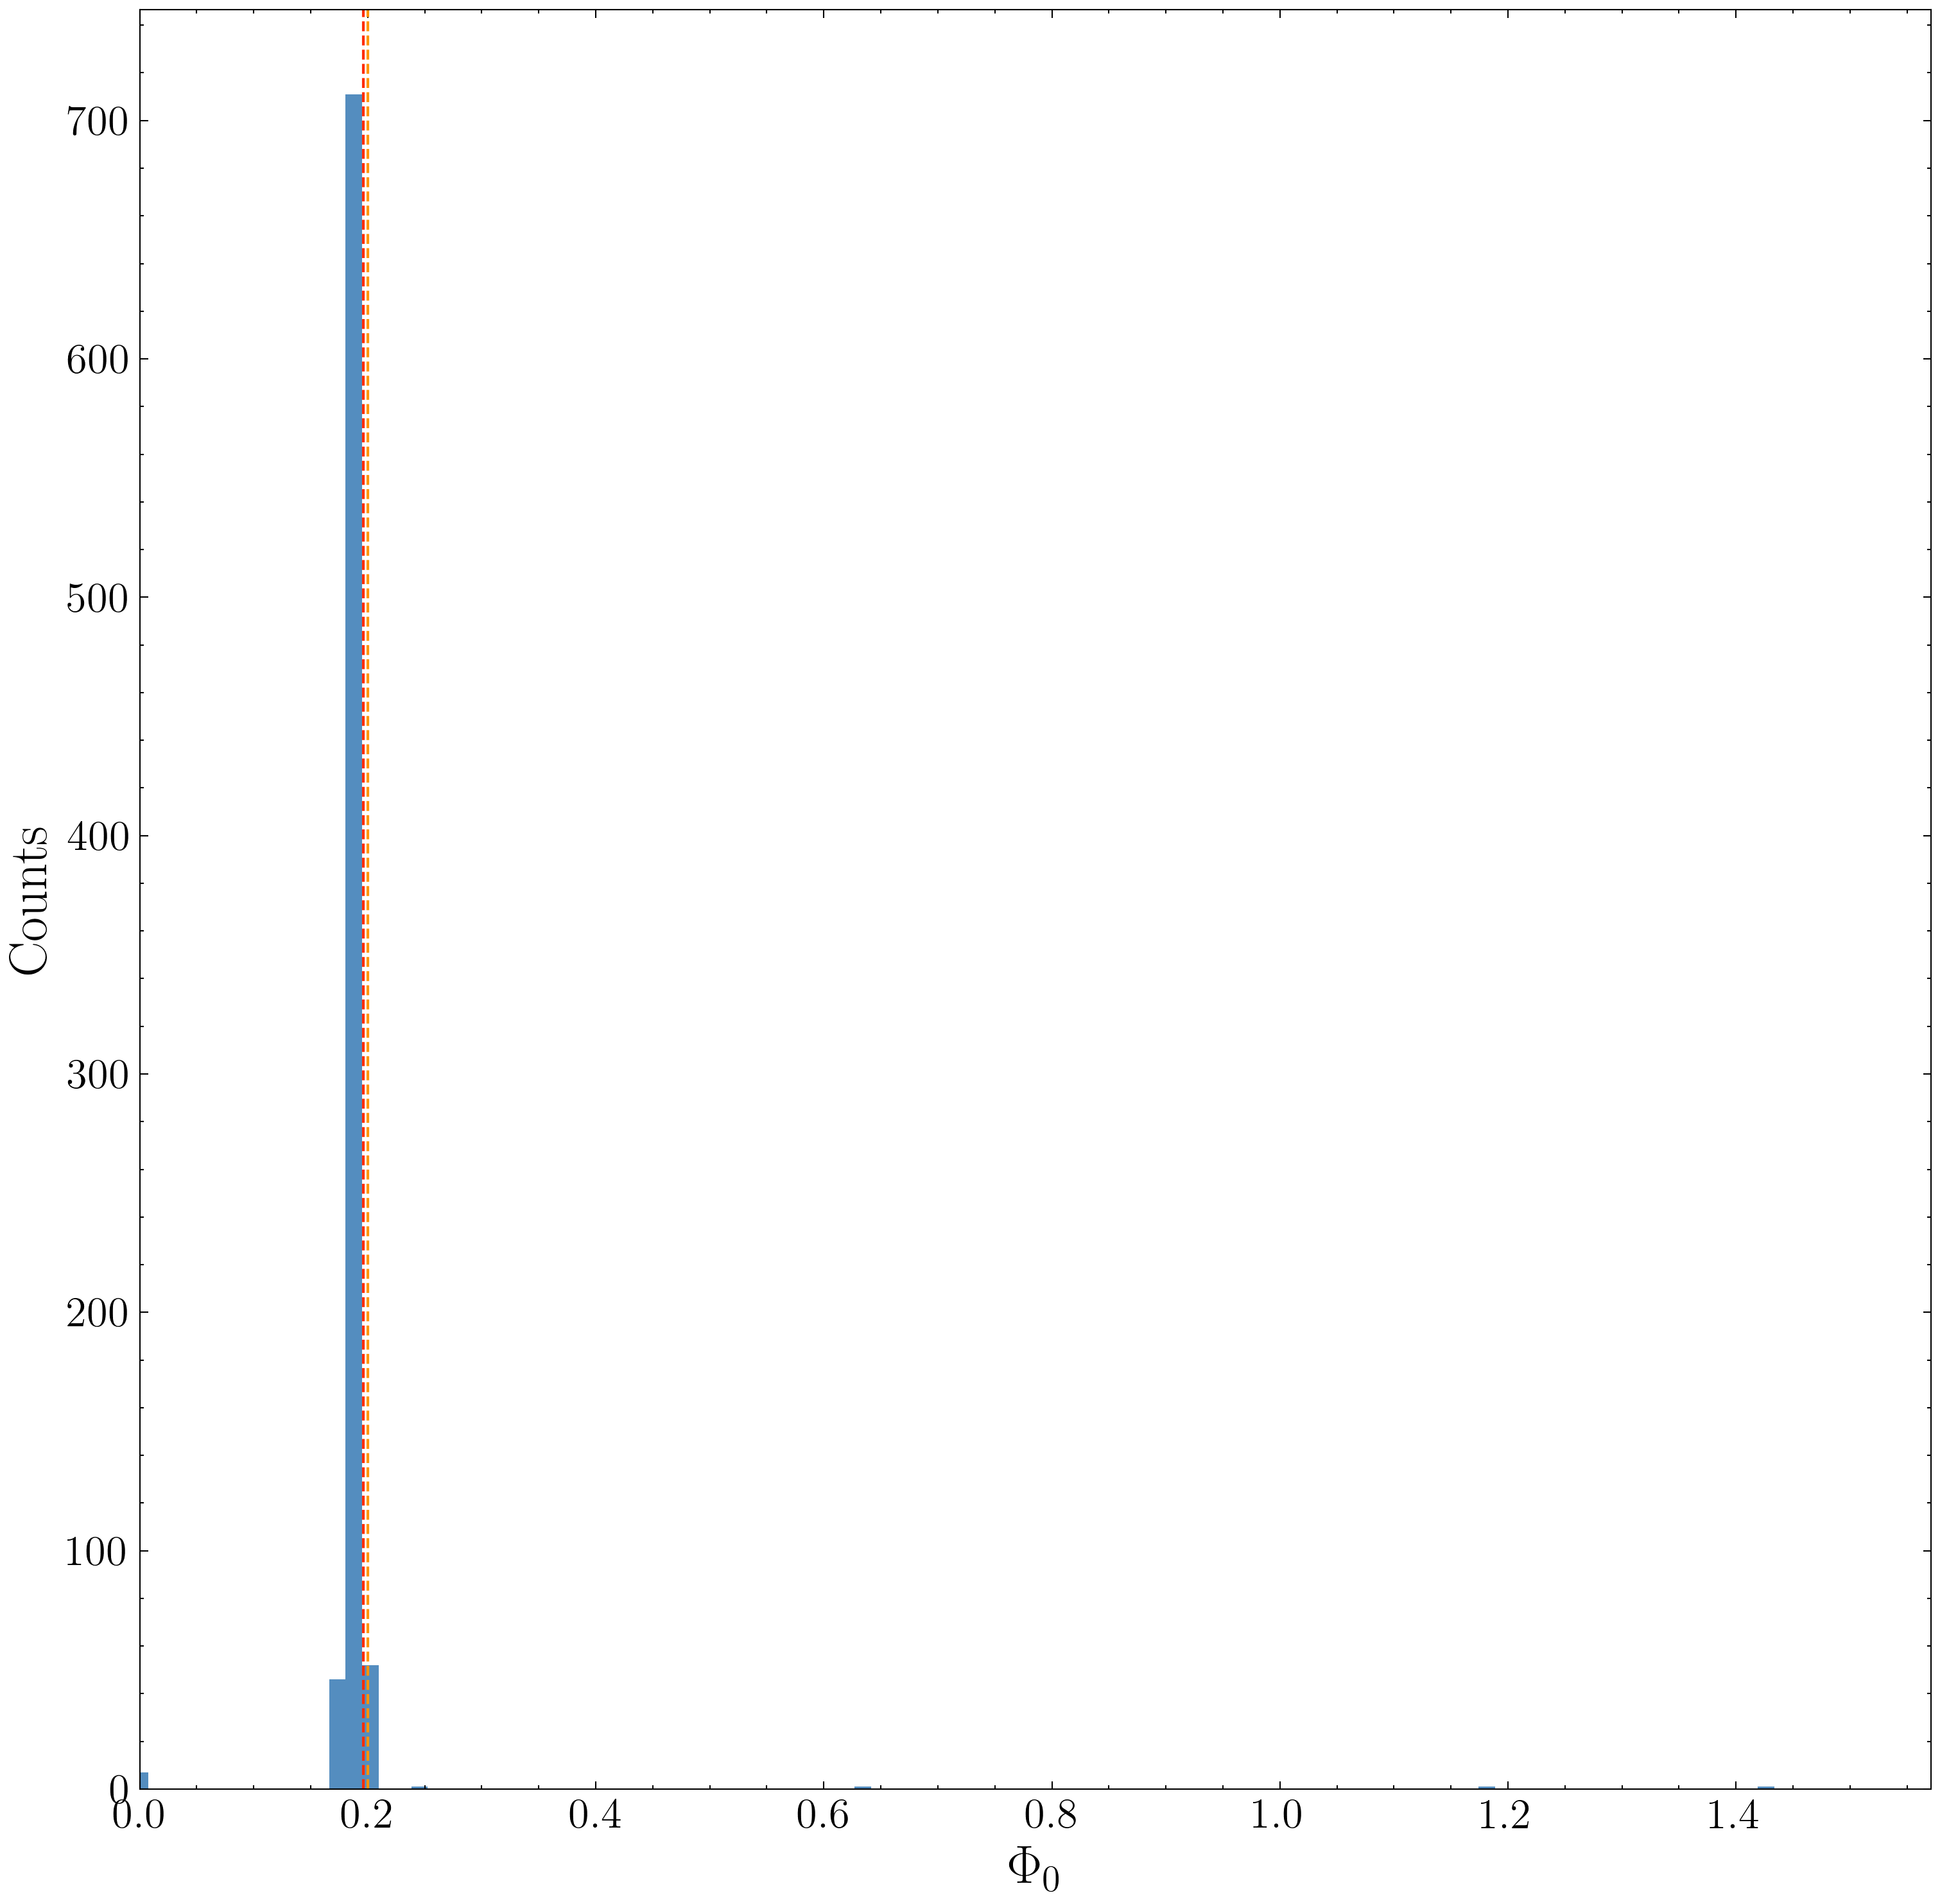
\includegraphics[width=\textwidth]{images/distribution_phi0_gw}
		\caption{$\Phi_0$}
	\end{subfigure}
	\hfill	
	\begin{subfigure}[b]{0.3\textwidth}
		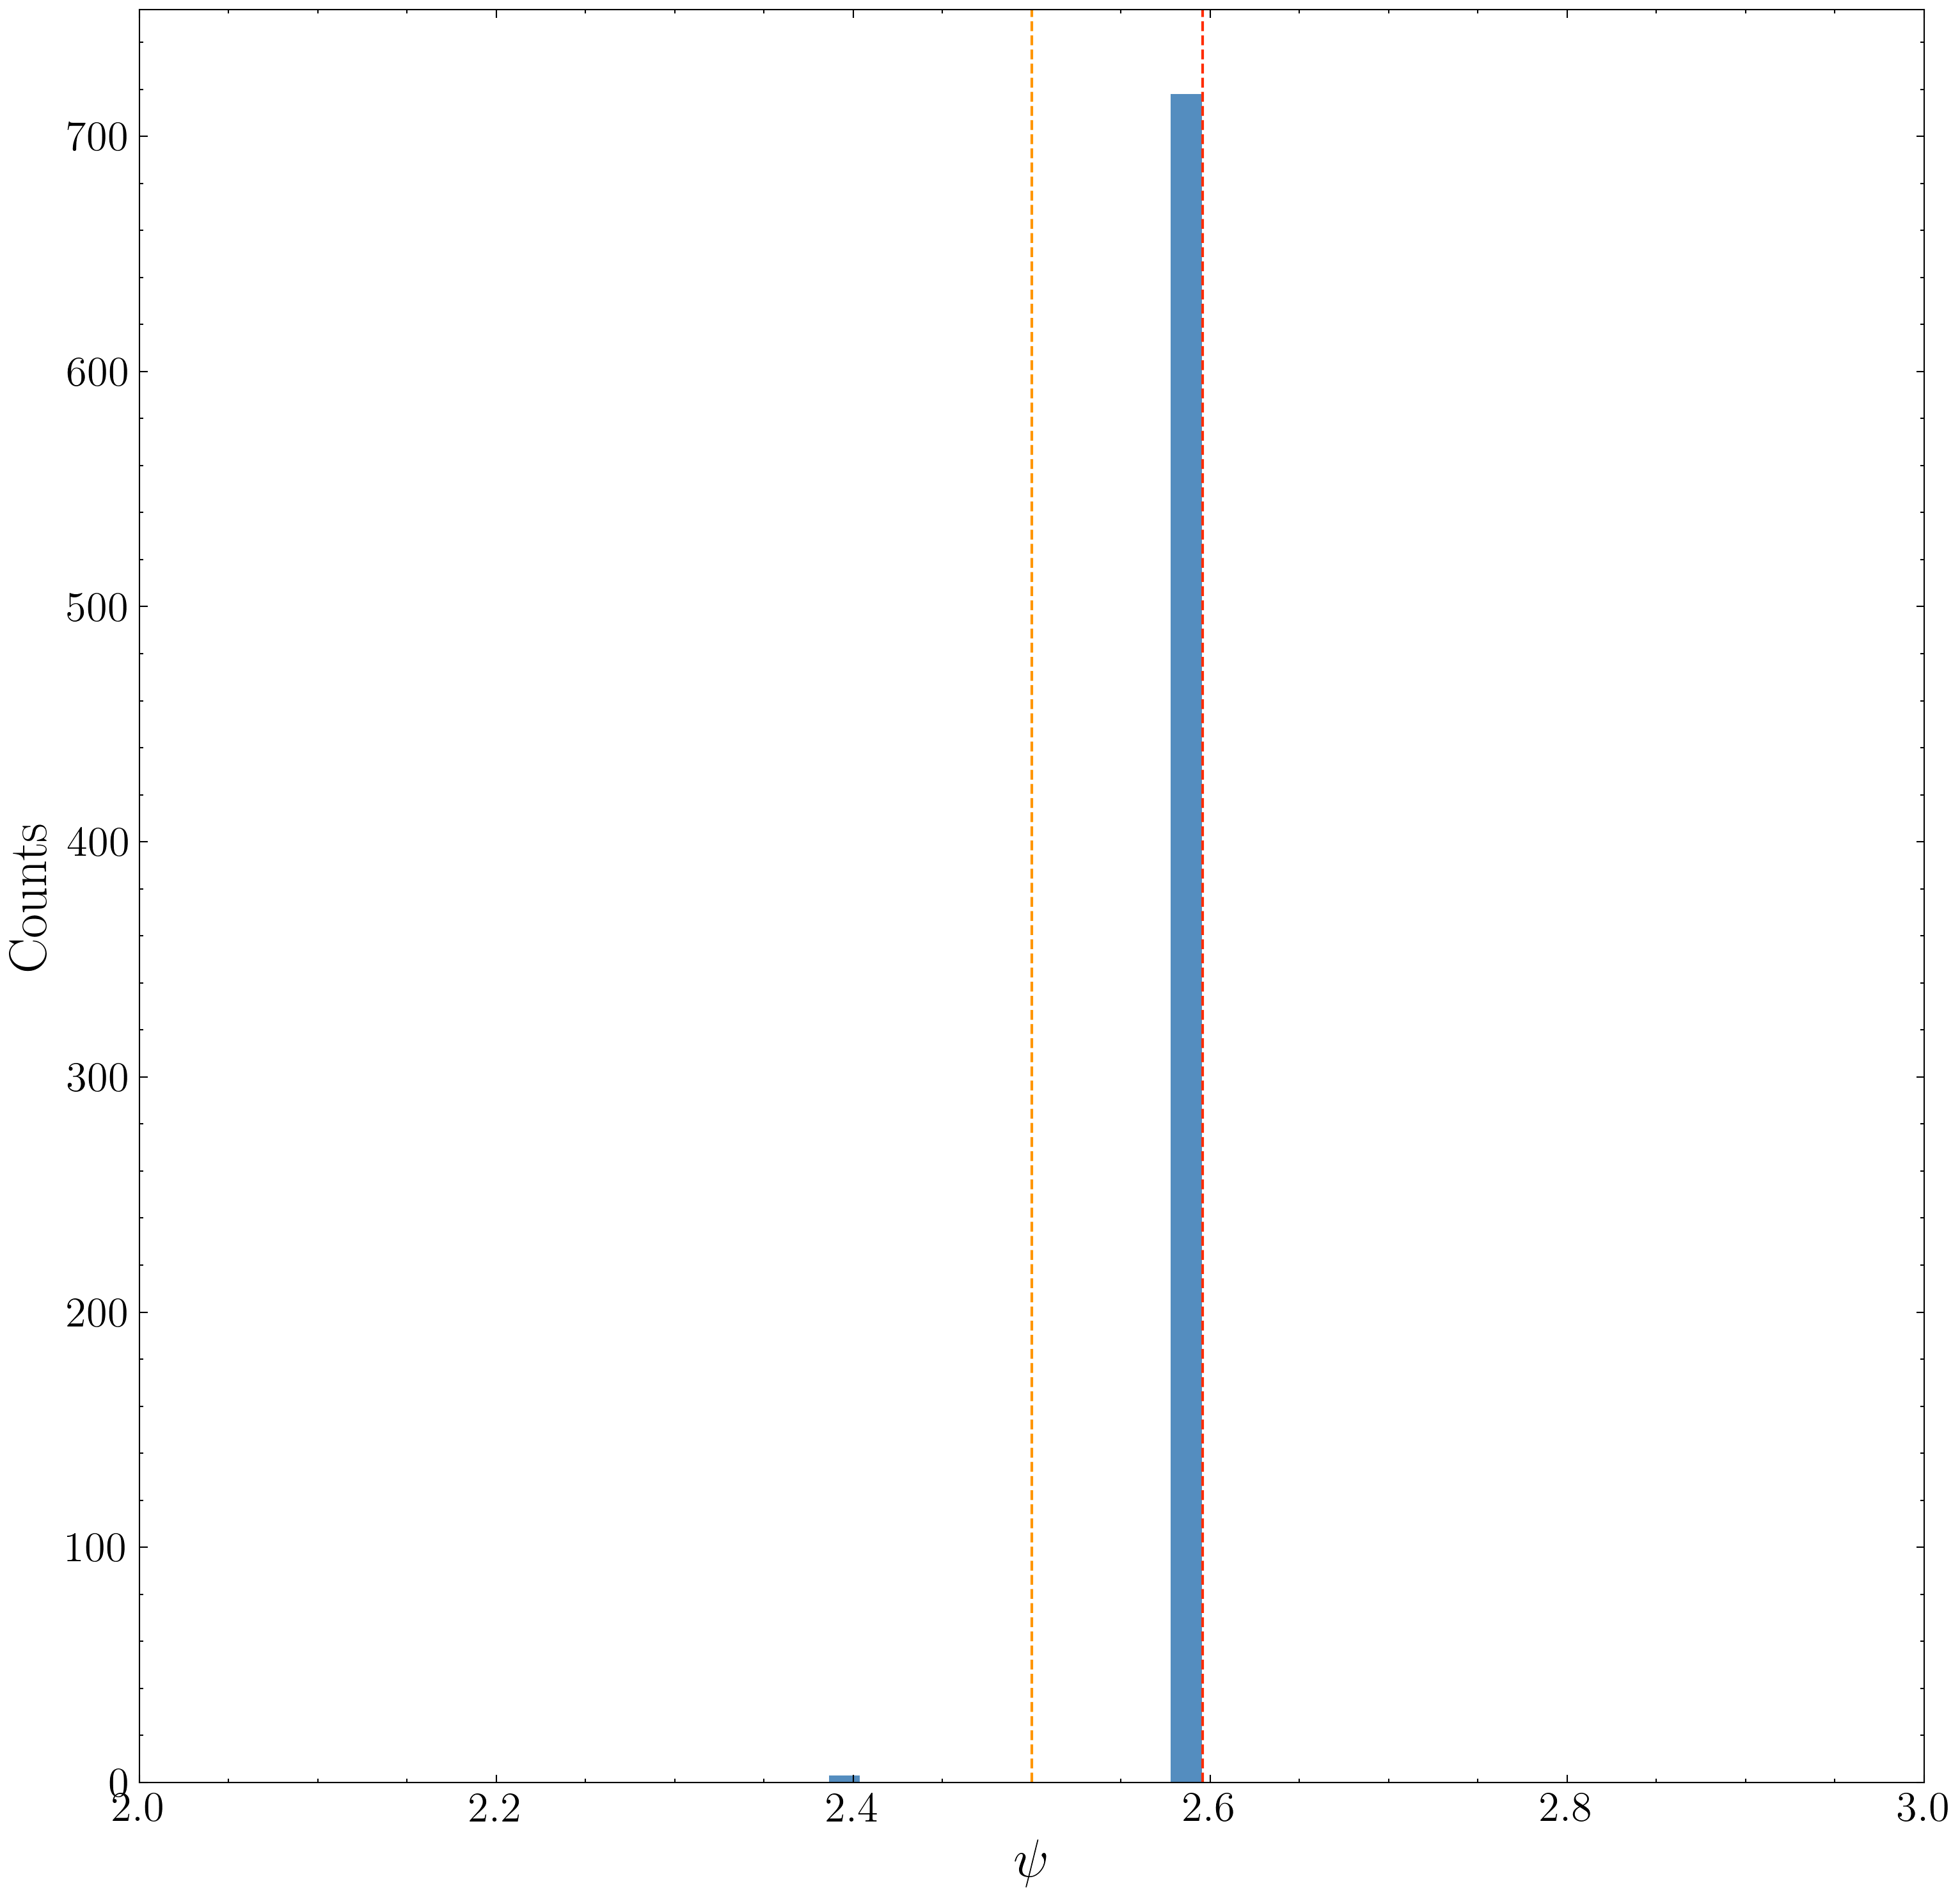
\includegraphics[width=\textwidth]{images/distribution_psi_gw}
		\caption{$\psi$}
	\end{subfigure}
	\medskip
	
	\begin{subfigure}[b]{0.3\textwidth}
		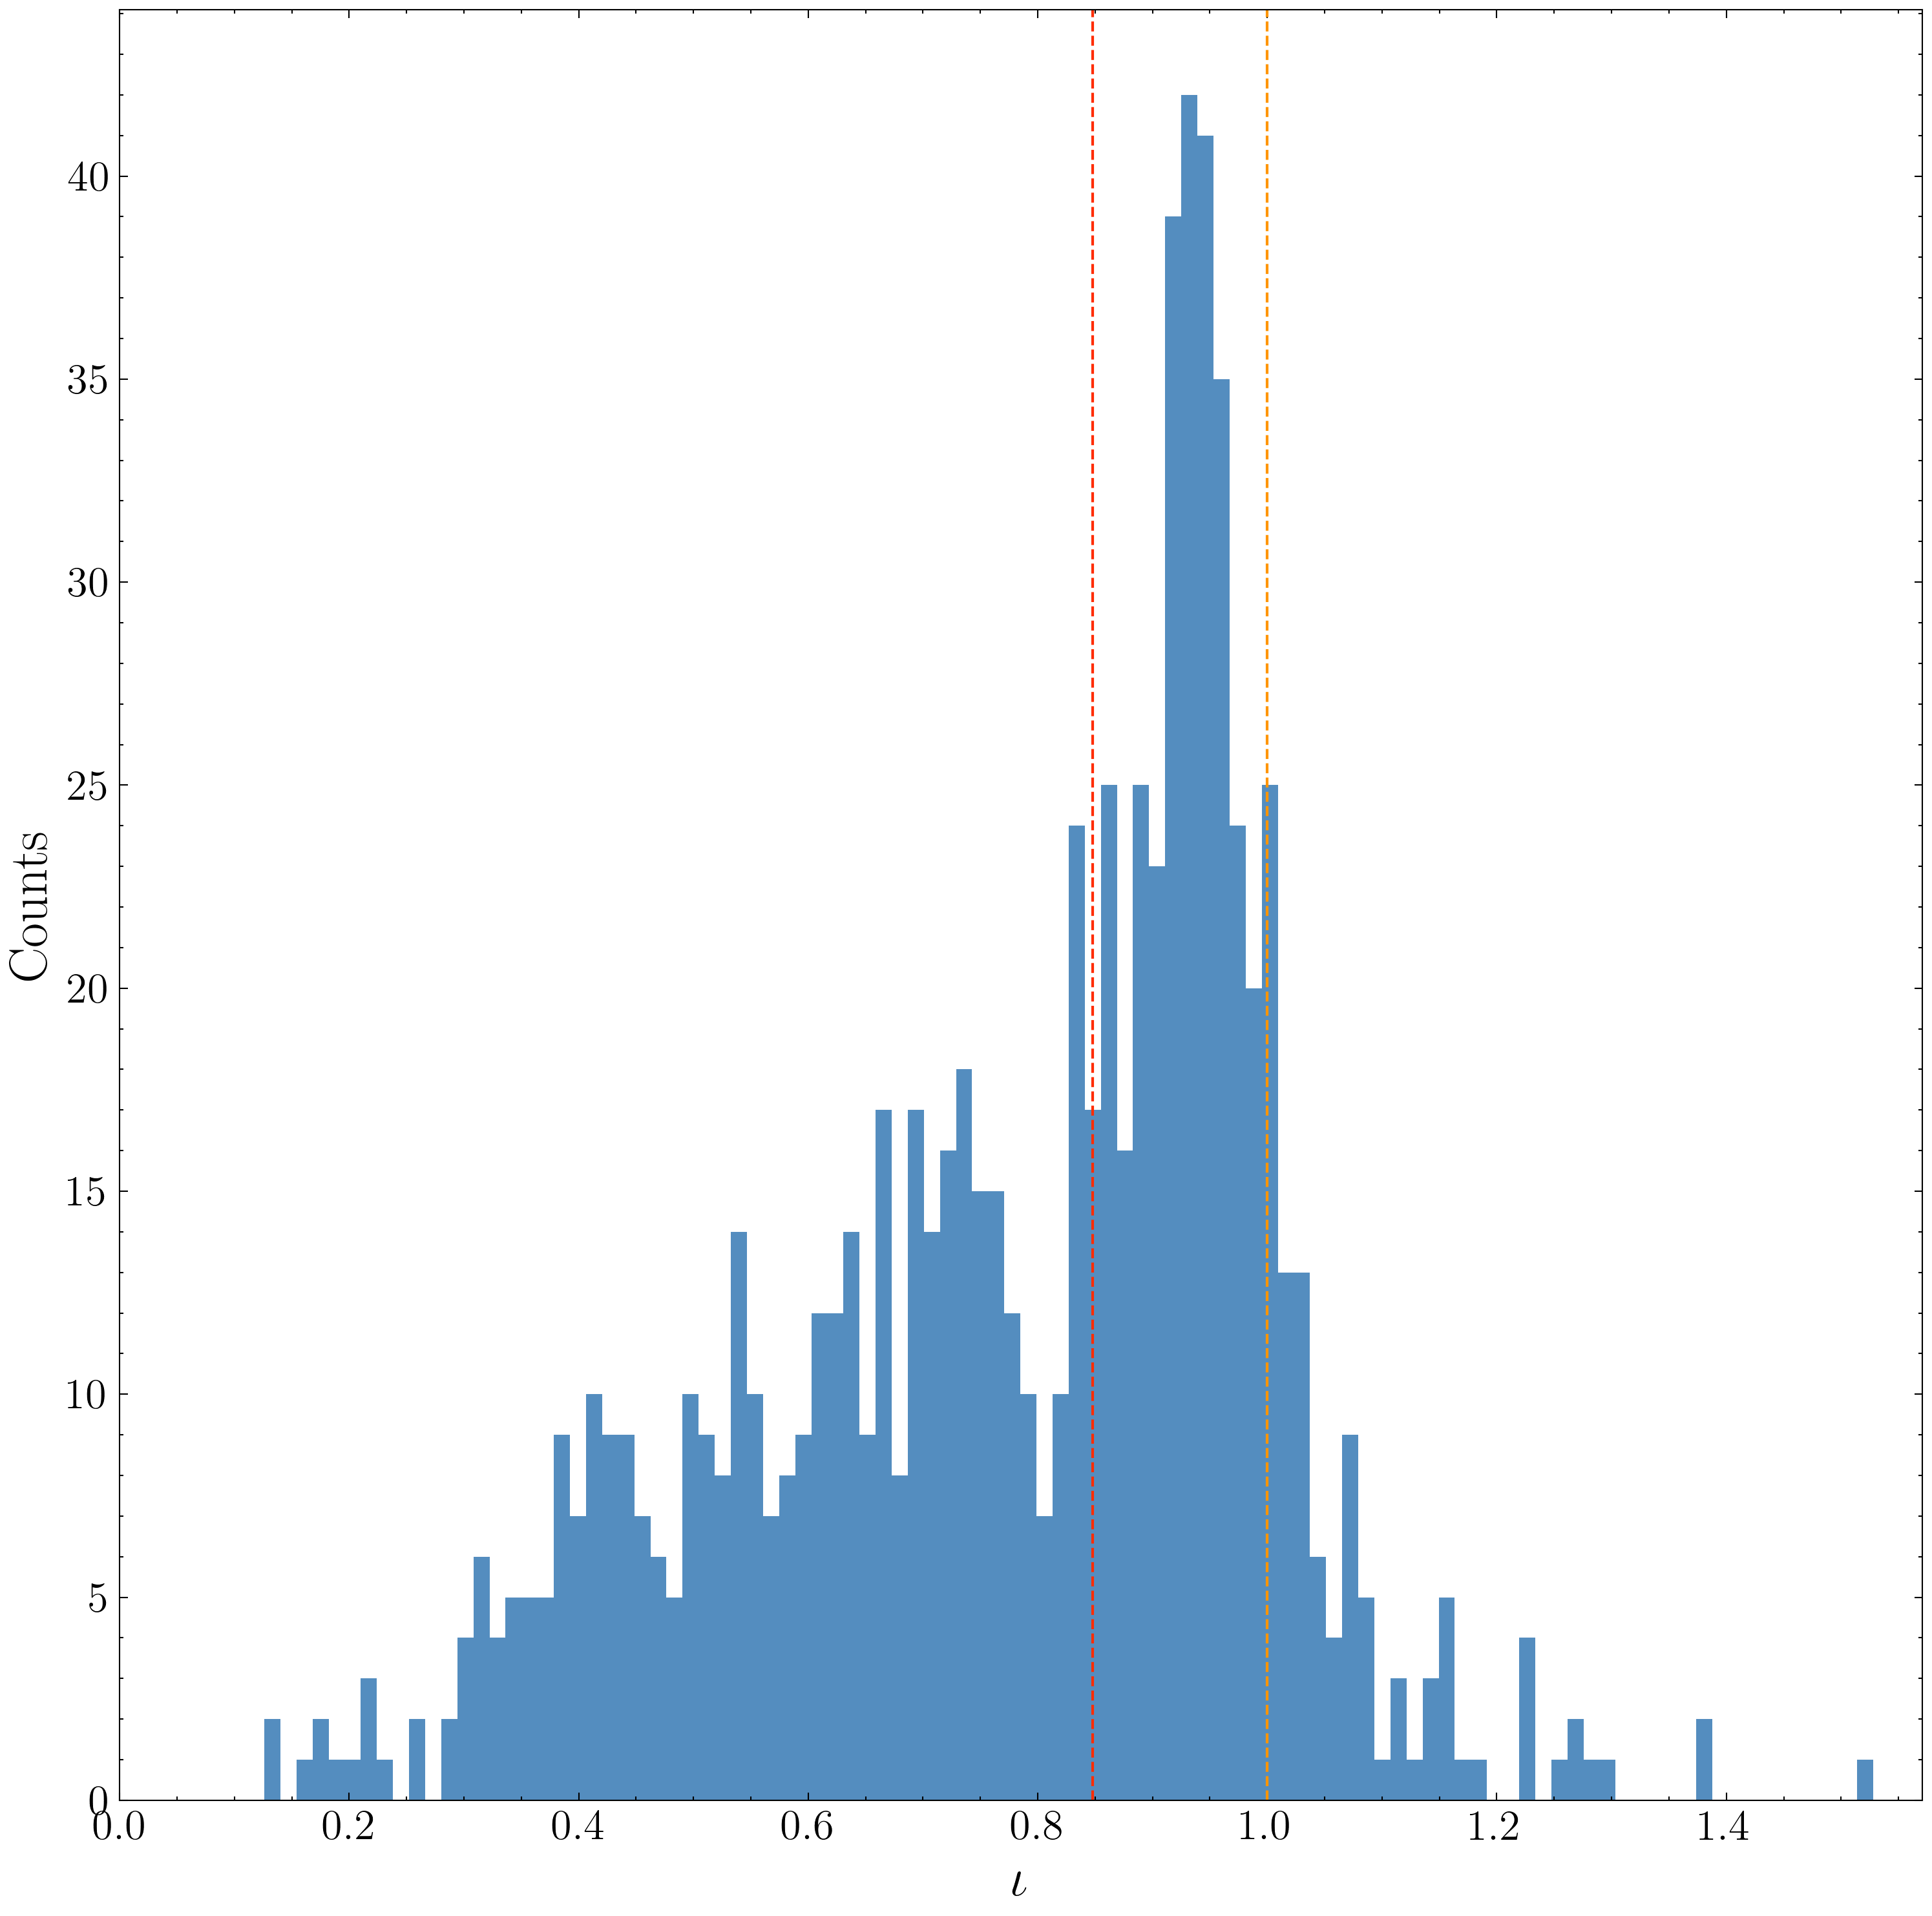
\includegraphics[width=\textwidth]{images/distribution_iota_gw}
		\caption{$\iota$}
	\end{subfigure}
	\hfill
	\begin{subfigure}[b]{0.3\textwidth}
		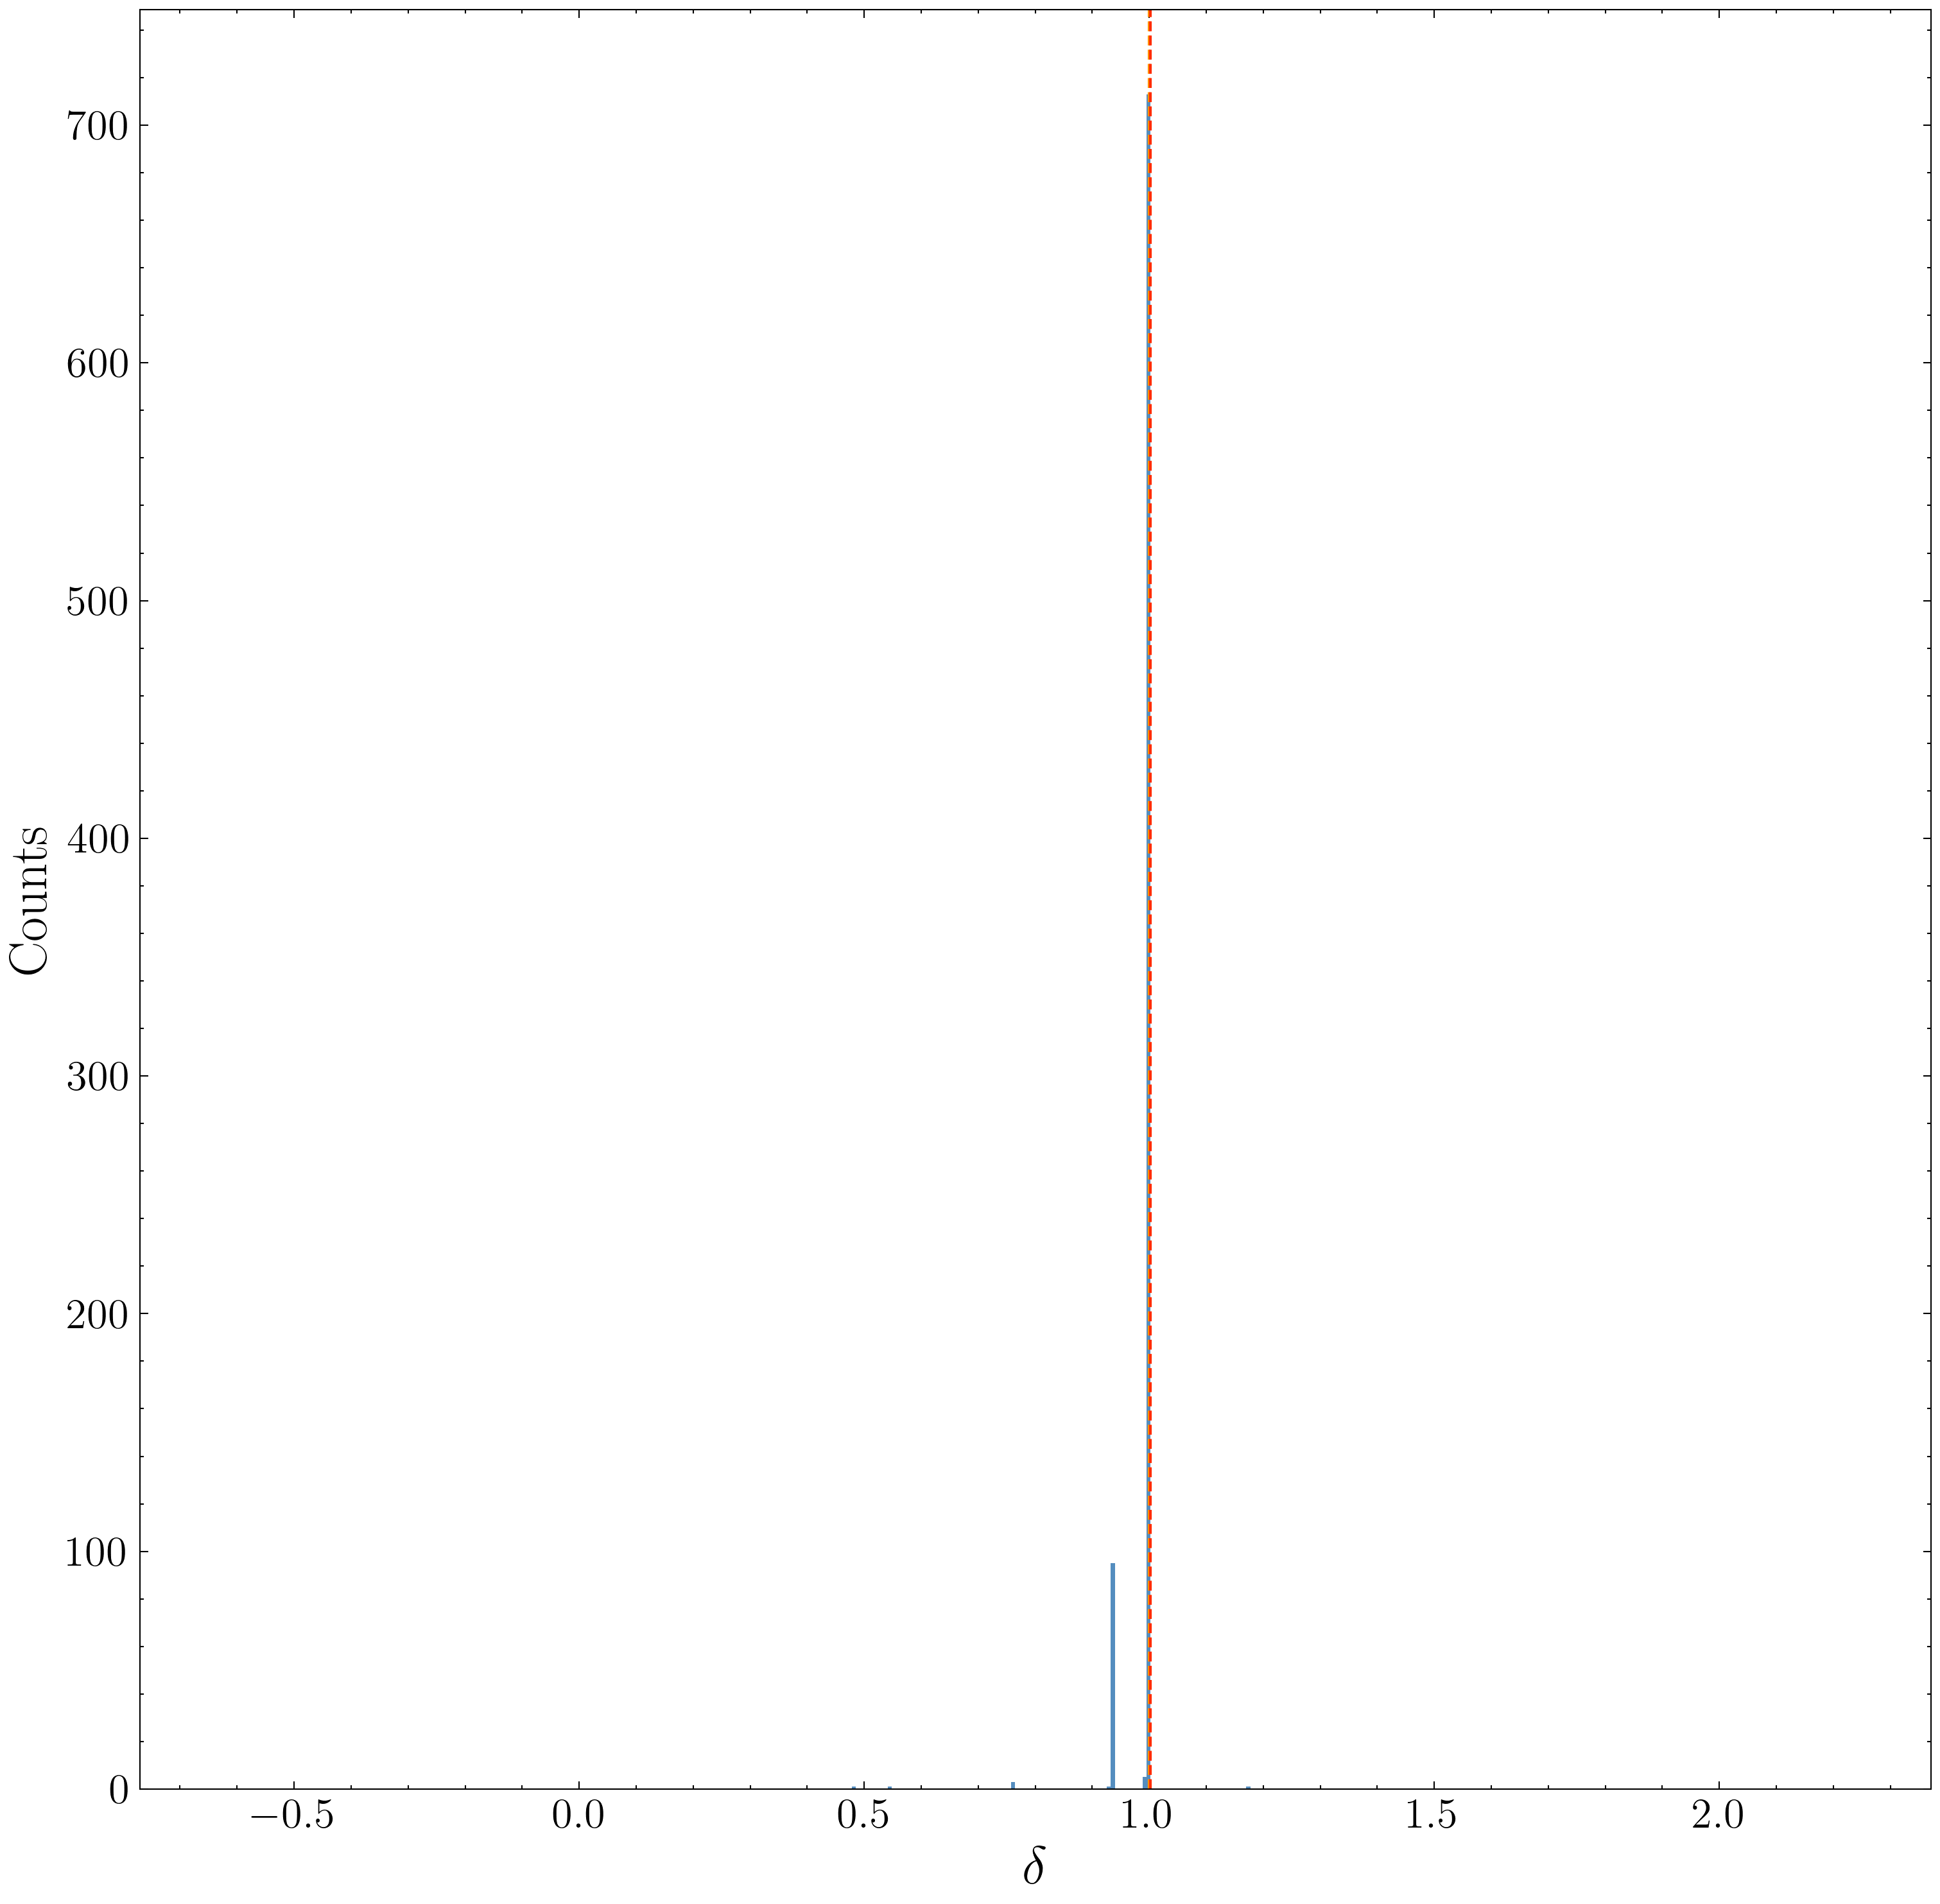
\includegraphics[width=\textwidth]{images/distribution_delta_gw}
		\caption{$\delta$}
	\end{subfigure}
	\hfill	
	\begin{subfigure}[b]{0.3\textwidth}
		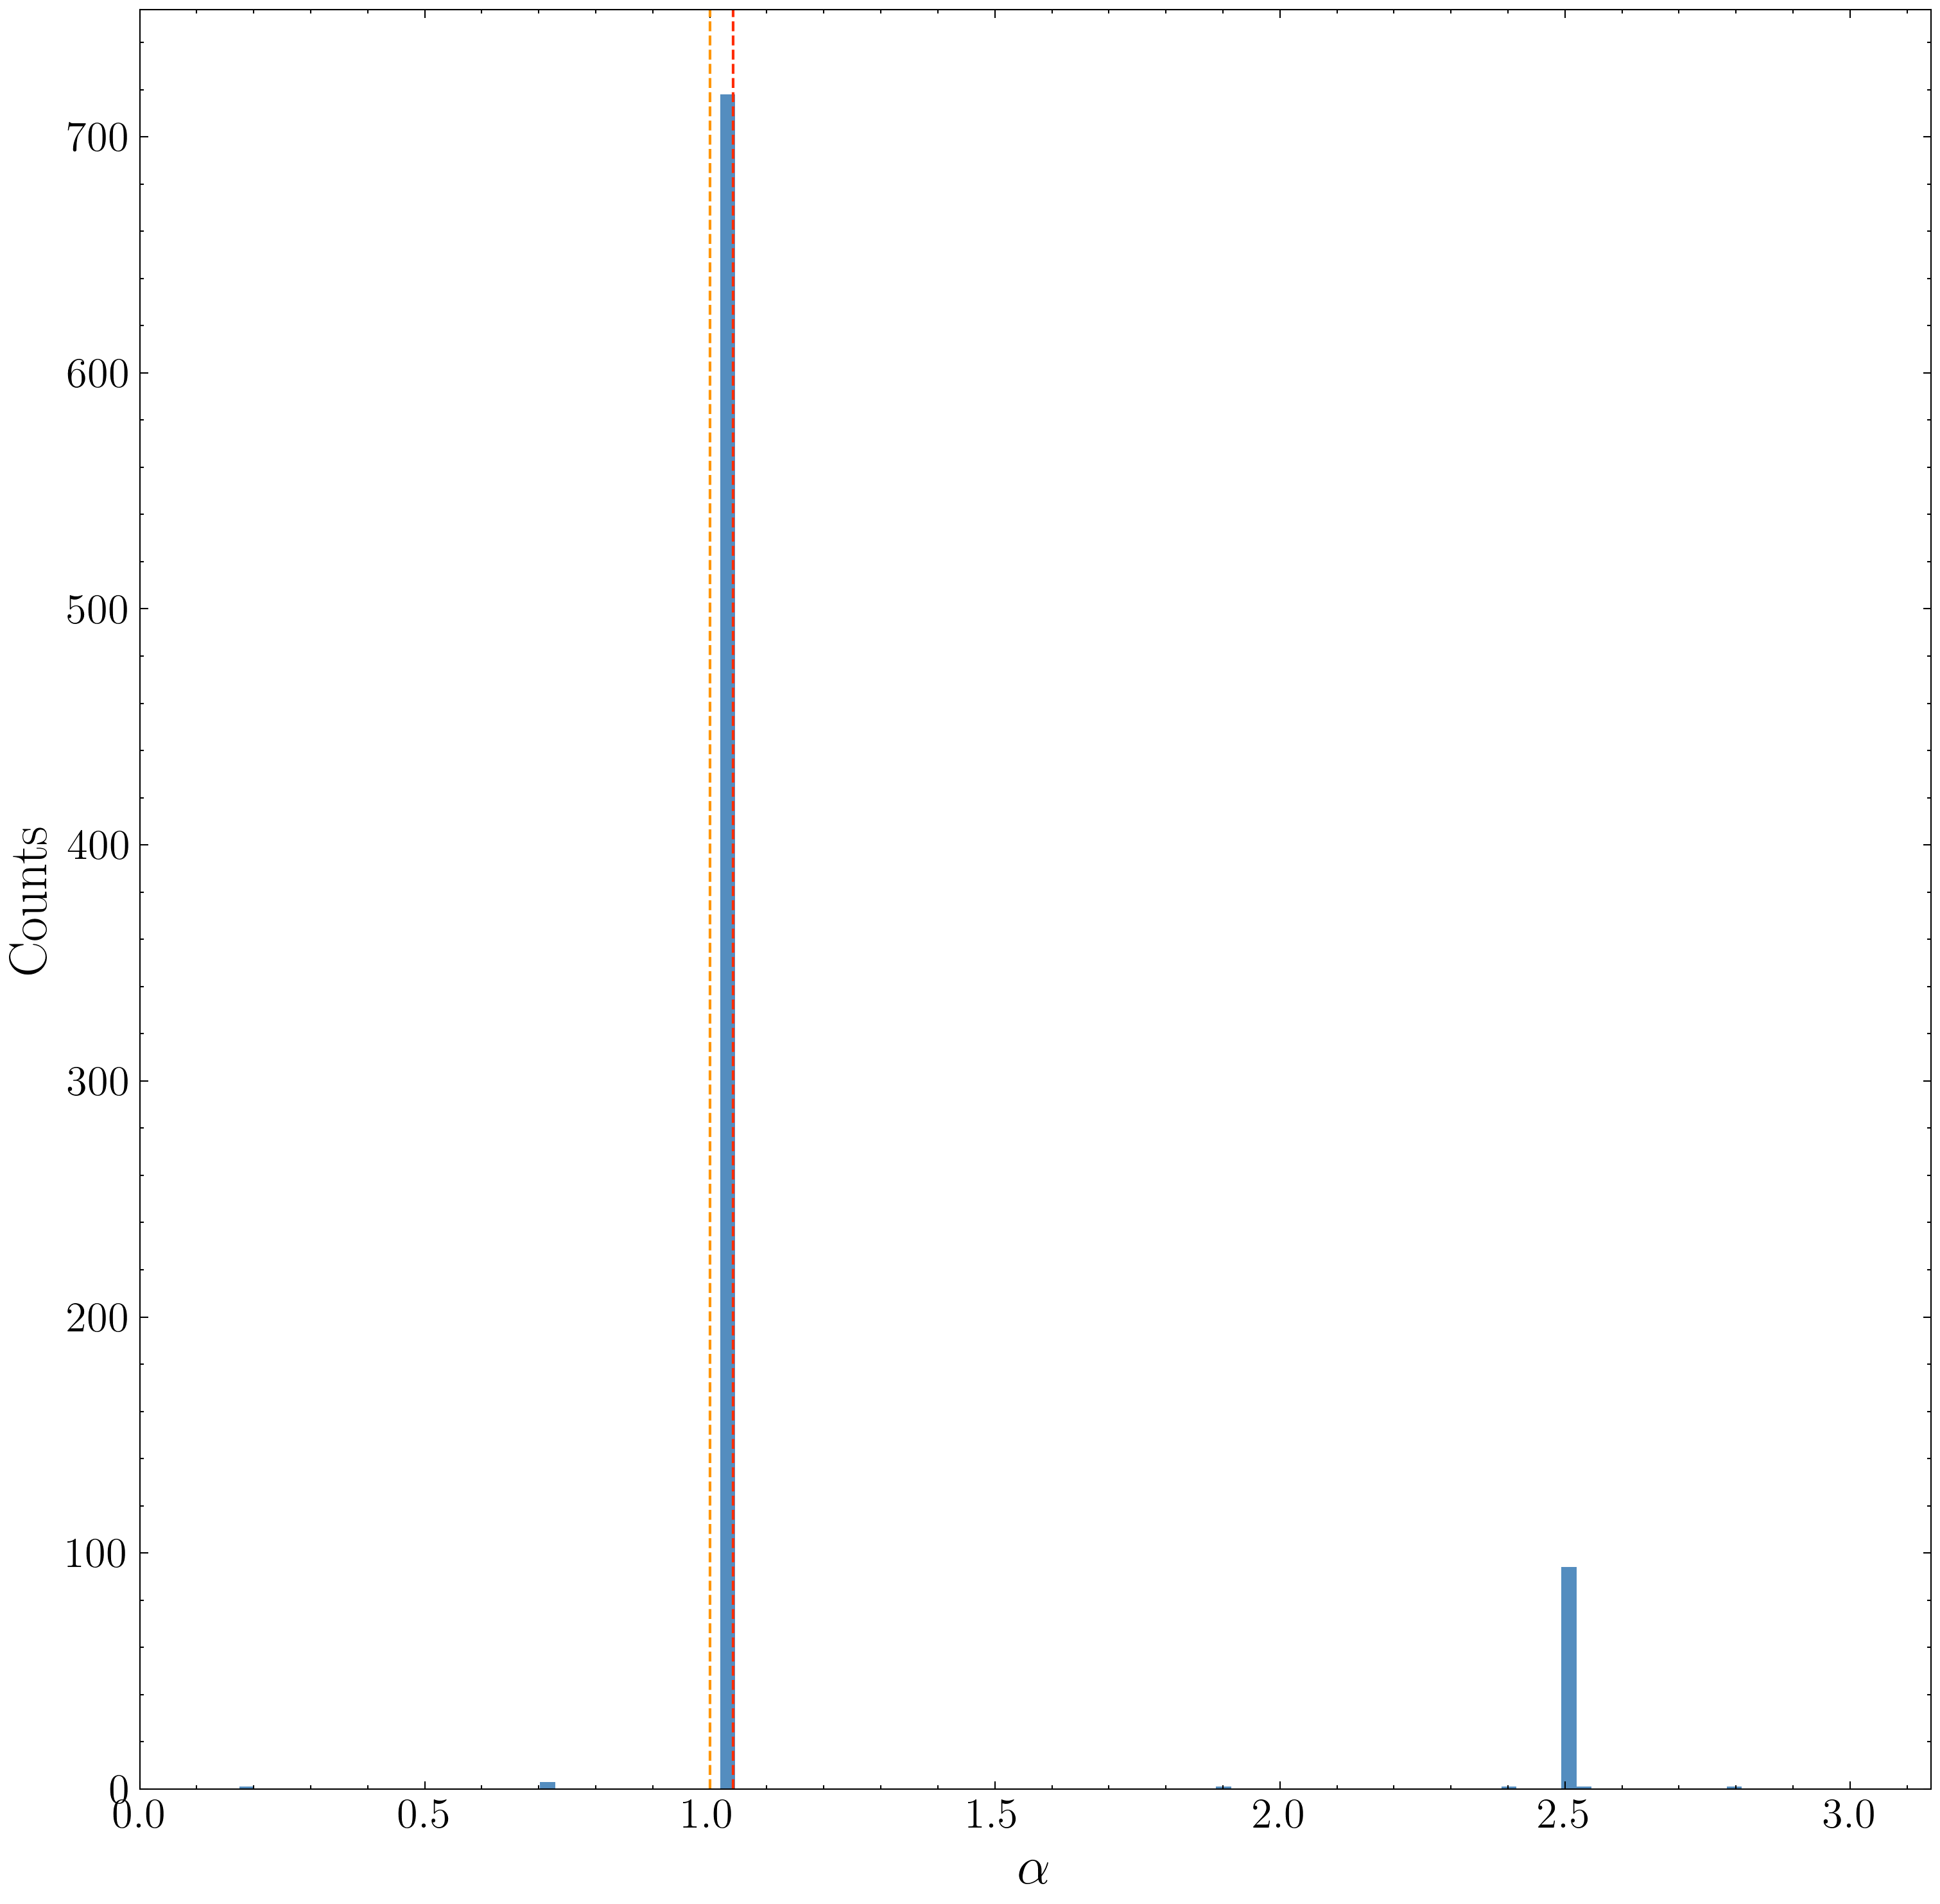
\includegraphics[width=\textwidth]{images/distribution_alpha_gw}
		\caption{$\alpha$}
	\end{subfigure}
	\medskip
	
	
	\medskip
	\begin{subfigure}[b]{0.33\textwidth}
		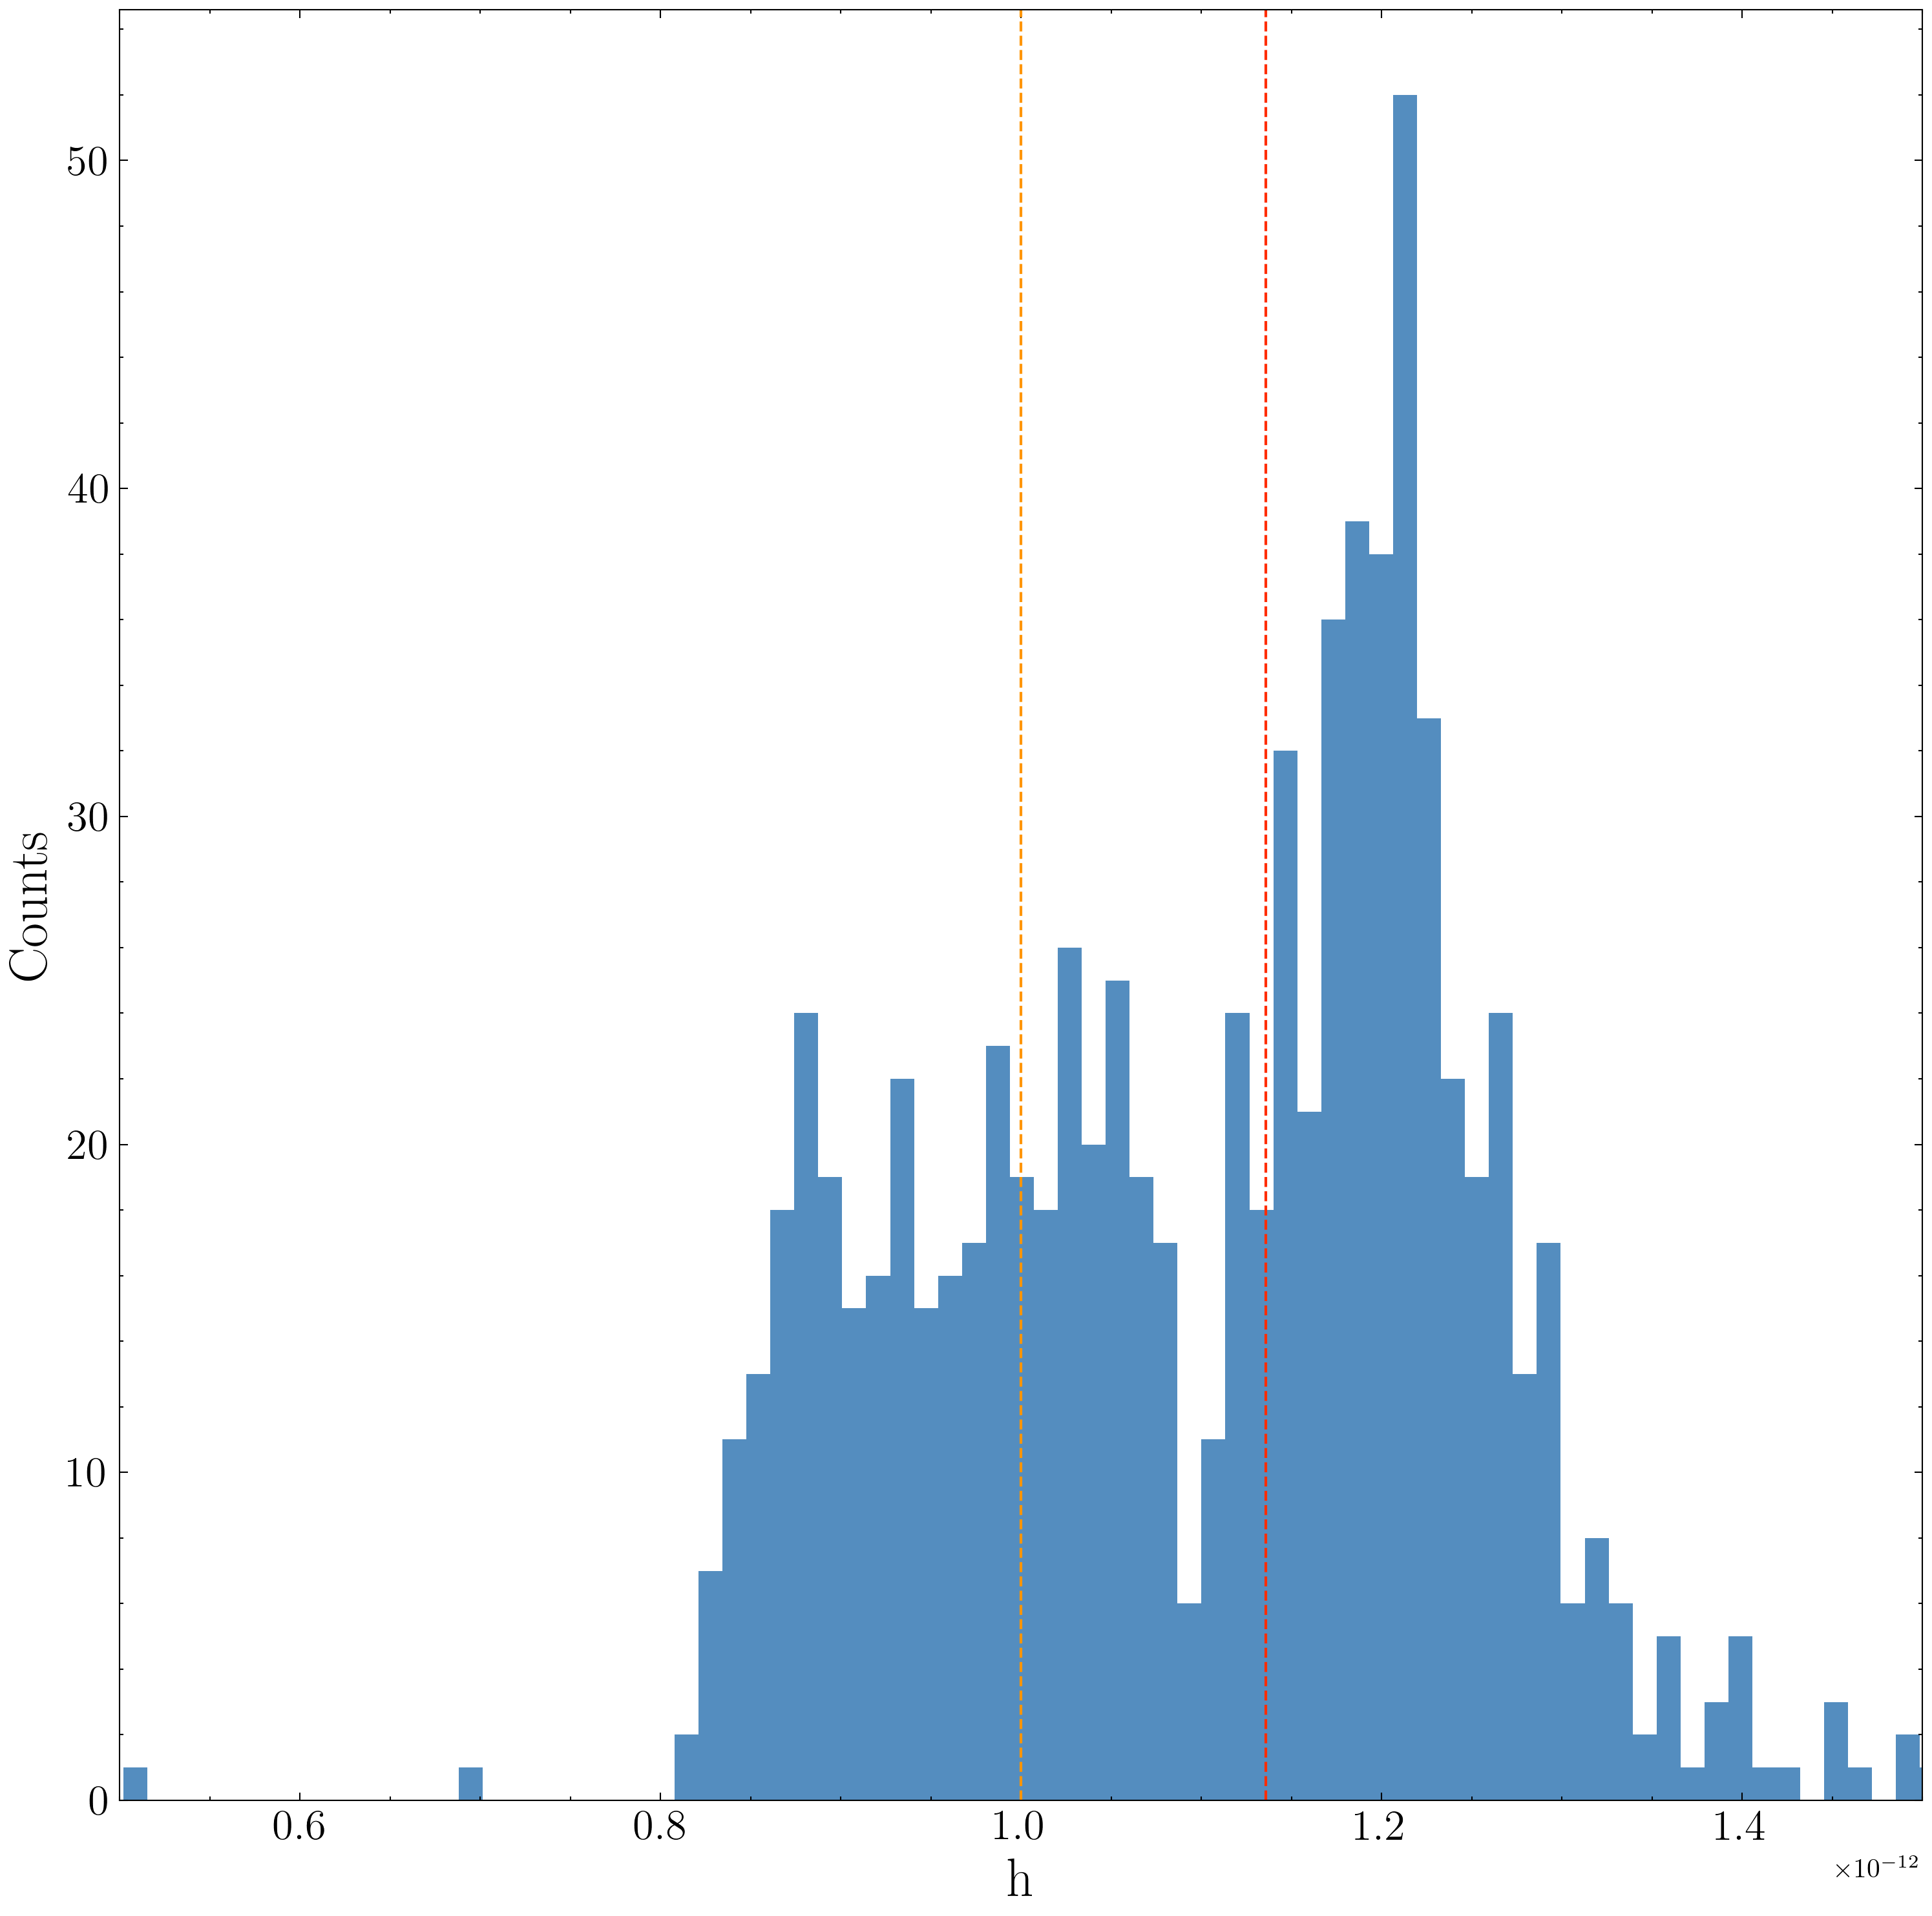
\includegraphics{images/distribution_h}
		\caption{$h$}
	\end{subfigure}
	
	\caption{Distribution in the median values of the 1D marginalized posteriors inferred by nested sampling for each static parameters of $\boldsymbol{\theta}_{\rm gw}$ over 1000 noise realisations. The orange dashed line labels the true injection value and the red dashed line labels the median of the distribution. \textcolor{red}{TK: these plots are ugly. Is there a better way to show this?}}\label{fig:median_distriubutins}
\end{figure*}
The above discussion was just for a single realisation of the noise processes. It is important to confirm that our method is robust against different realisations of the noise and that the specific realisation of the noisy data used in Sections \ref{sec:parameter_estim}, \ref{sec:detection} is not particularly advantageous or convenient for our method. To this end we take our representative example from Table \ref{tab:parameters_and_priors} and generate 1000 realisations of the process noise and measurement noise. For each realisation of the data we can then independently estimate the static parameters, $\boldsymbol{\theta}$. In Figure \ref{fig:corner_plot_2} we show the results for the  estimated values of $\boldsymbol{\theta}_{\rm gw}$ for 9 realisations of the noise. This figure is analogous to the single noise realisation of Figure \ref{fig:corner_plot_1}. We plot only 9 realisations of the noise rather than the full set of 1000 realisations so as to not overcrowd the figure. We can see from Figure \ref{fig:corner_plot_2} that the results for multiple noise realisations agree well with the results that we saw in  Figure \ref{fig:corner_plot_1} for a single noise realisation. The estimates of the parameters $\Omega, \Phi_0, \psi, \delta$ and $\alpha$ are highly consistent across the different noise realisations i.e. the variance between the different marginalized posteriors is generally low. The estimates generally agree with the injected values with high fidelity. Conversely, for the parameters $\iota$ and $h_0$ the variance between the different marginalized posteriors is generally high; we infer highly different estimates of these parameters depending on the particular realisation of the noise. Similar to the estimates of $\boldsymbol{\theta}_{\rm gw}$, the estimates of $\boldsymbol{\theta}_{\rm psr}$ (c.f.  Fig \ref{fig:example_psr_params}) show a consistency across multiple noise realisations, though for brevity we do not show the results here \textcolor{red}{TK: is this fair? Don't want to clog up paper with extra figures that don't offer any additional insight...} \newline   
 
The large degree of variance in the estimates of $\iota$ and $h_0$ is due to the nested sampling algorithm effectively trading off accuracy in one parameter against the accuracy in other. From Eqs. \ref{eq:hphx}, \ref{eq:hphx2} we can see that there is a weak degeneracy between $\iota$ and $h$. For example, from Eq \ref{eq:hphx2} it is not clear if a larger value of the cross polarisation strain $h_{\times}$ is due to the system having a larger strain amplitude $h_0$, or a different inclination $\iota$. This degeneracy is broken generally by the relation for $h_{+}$, Eq \ref{eq:hphx}. Whilst this ensures that both parameters are then generally identifiable formally, in practice an identifiability issue persists since the log-likelihood surface in $\iota -h_0$ space plateaus across a broad range of physically reasonable values (\textcolor{red}{TK: Could include a figure here showing this, but don't want to overclutter}).  Consequently it is difficult for our algorithm to select a particular point in this plateau. If we fix one of the parameters at its true value, taking a slice through the likelihood surface, it is then possible to identify a particular point in the plateau and the variance in the estimates between different noise realisations decreases. This is demonstrated in Figure \ref{fig:iota} where we plot the marginalized 1D posterior of $\iota$ for 9 realisations of the noise in both the original case where $h_0$ is a free parameter (i.e. Figure \ref{fig:corner_plot_2}) and in the case where we hold $h_0$ fixed at its injection value, $h_0 = 10^{-12}$. We can see that whilst the variance between the individual posteriors is large in the original case, once we fix $h_0$ the variance decreases dramatically and the sampling algorithm repeatedly converges consistent estimates of $\iota$. There is a notable bias in Figure \ref{fig:iota} in the estimates for $\iota$ inferred for the fixed $h_0$ case relative to the true injected value; whilst the variance has decreased, the mean accuracy of the estimates has also decreased. This bias is a result of dropping the pulsar terms from our measurement equation and is discussed in Section \ref{sec:bias}. \newline 

For each realisation of the noise we infer a marginalised 1-D posterior for each parameter. In turn, each posterior distribution has a median value. We plot the distribution of these medians over the 1000 noise realisations for each parameter of $\boldsymbol{\theta}_{\rm gw}$ in Figure \ref{fig:median_distriubutins}. For each of these distributions we can also calculate the median value (i.e. the median of the medians) and compare it with the true injection value. This is shown by the red and orange dashed lines respectively in the Figure. Analogous to the results we saw in Figure \ref{fig:corner_plot_2}, the distributions of the median values of the parameters $\Omega, \Phi_0, \psi, \delta$ and $\alpha$ are very narrow, with a generally small discrepancy between the inferred value and the injected value. Conversely, the distributions for $\iota$ and $h_0$ are much broader and exhibit a bias of $\sim 0.18$ radians and $0.17 \times 10^{-12}$ respectively. This agrees with the results we discussed for the 9 noise realisations in Figure \ref{fig:corner_plot_2} where a bias in $\iota$ and $h_0$ was also observed. In addition to  $\iota$ and $h_0$  exhibiting a strong bias, the parameters $\psi$ and $\alpha$ also exhibit a small bias of magnitude $\sim 0.1$ and $\sim 0.04$ radians respectively. This bias is again a result of dropping the pulsar terms from the measurement equation and will be discussed in Section \ref{sec:bias}. 




\subsection{Exploring a broader parameter space} \label{sec:parameter_space}

\textcolor{red}{TK: TBD. Maybe lets just change the sky position - it it too expensive to generate a sky map of minimum detectable strain. Given the biases I don't know if a PP plot quite makes sense at this stage...}



\subsection{Bias by dropping pulsar terms}\label{sec:bias}
Evident in the preceding discussion is the fact that for some of the $\boldsymbol{\theta}_{\rm gw}$ parameters the inferred value (i.e. the median of the 1D marginalised posterior) is biased away from the true injection value. This effect is most severe for $\iota$ and $h_0$ (e.g. Figures \ref{fig:iota}, \ref{fig:median_distriubutins}) but also present to a lesser extent in other static parameters such as $\alpha$ and $\psi$. In this Section we demonstrate how this bias results from the dropping of the pulsar terms described in Section \ref{sec:parameter_estim}.


In Figure \ref{fig:likelihood_curves_earth} we plot the variation in the log-likelihood returned by the Kalman filter, Eq. \ref{eq:likelihood}, as we vary a single static parameter of $\boldsymbol{\theta}_{\rm gw}$, holding all other parameters constant at their true injected value. For instance, in Figure \ref{fig:omega_likelihood} we pass different values of $\Omega$ in the range $10^{-9}$ to $10^{-5}$ Hz into the Kalman filter, whilst holding the remaining parameters constant, and plot the retuned log-likelihood as a function of $\Omega$. The dashed orange line labels the true injection value whilst the dashed red line labels the location of the maximum log-likelihood. Finding the location of this maximum across all parameters is effectively the goal of any likelihood based inference method, such as nested sampling. 



The key observation from Figure \ref{fig:likelihood_curves_earth} is that for many parameters the location of the likelihood optima and the location of the injected value are not the same, that is, the orange and red dashed lines are not coincident. 



This feature shows up as a bias in 




Taking a specific example, in Figure \ref{fig:iota_likelihood}
Consequently 







Indeed this is a 1D representation of a multidimensinal problem and the exact shape of the likelihood curves depends on the 








Whilst the earth term likelihoo dcurves are generally smooth...










If the effect is present in our analysis, also present in other analysis?





\begin{figure*}
	\setkeys{Gin}{width=\linewidth}   
	
	\begin{subfigure}[b]{0.22\textwidth}
		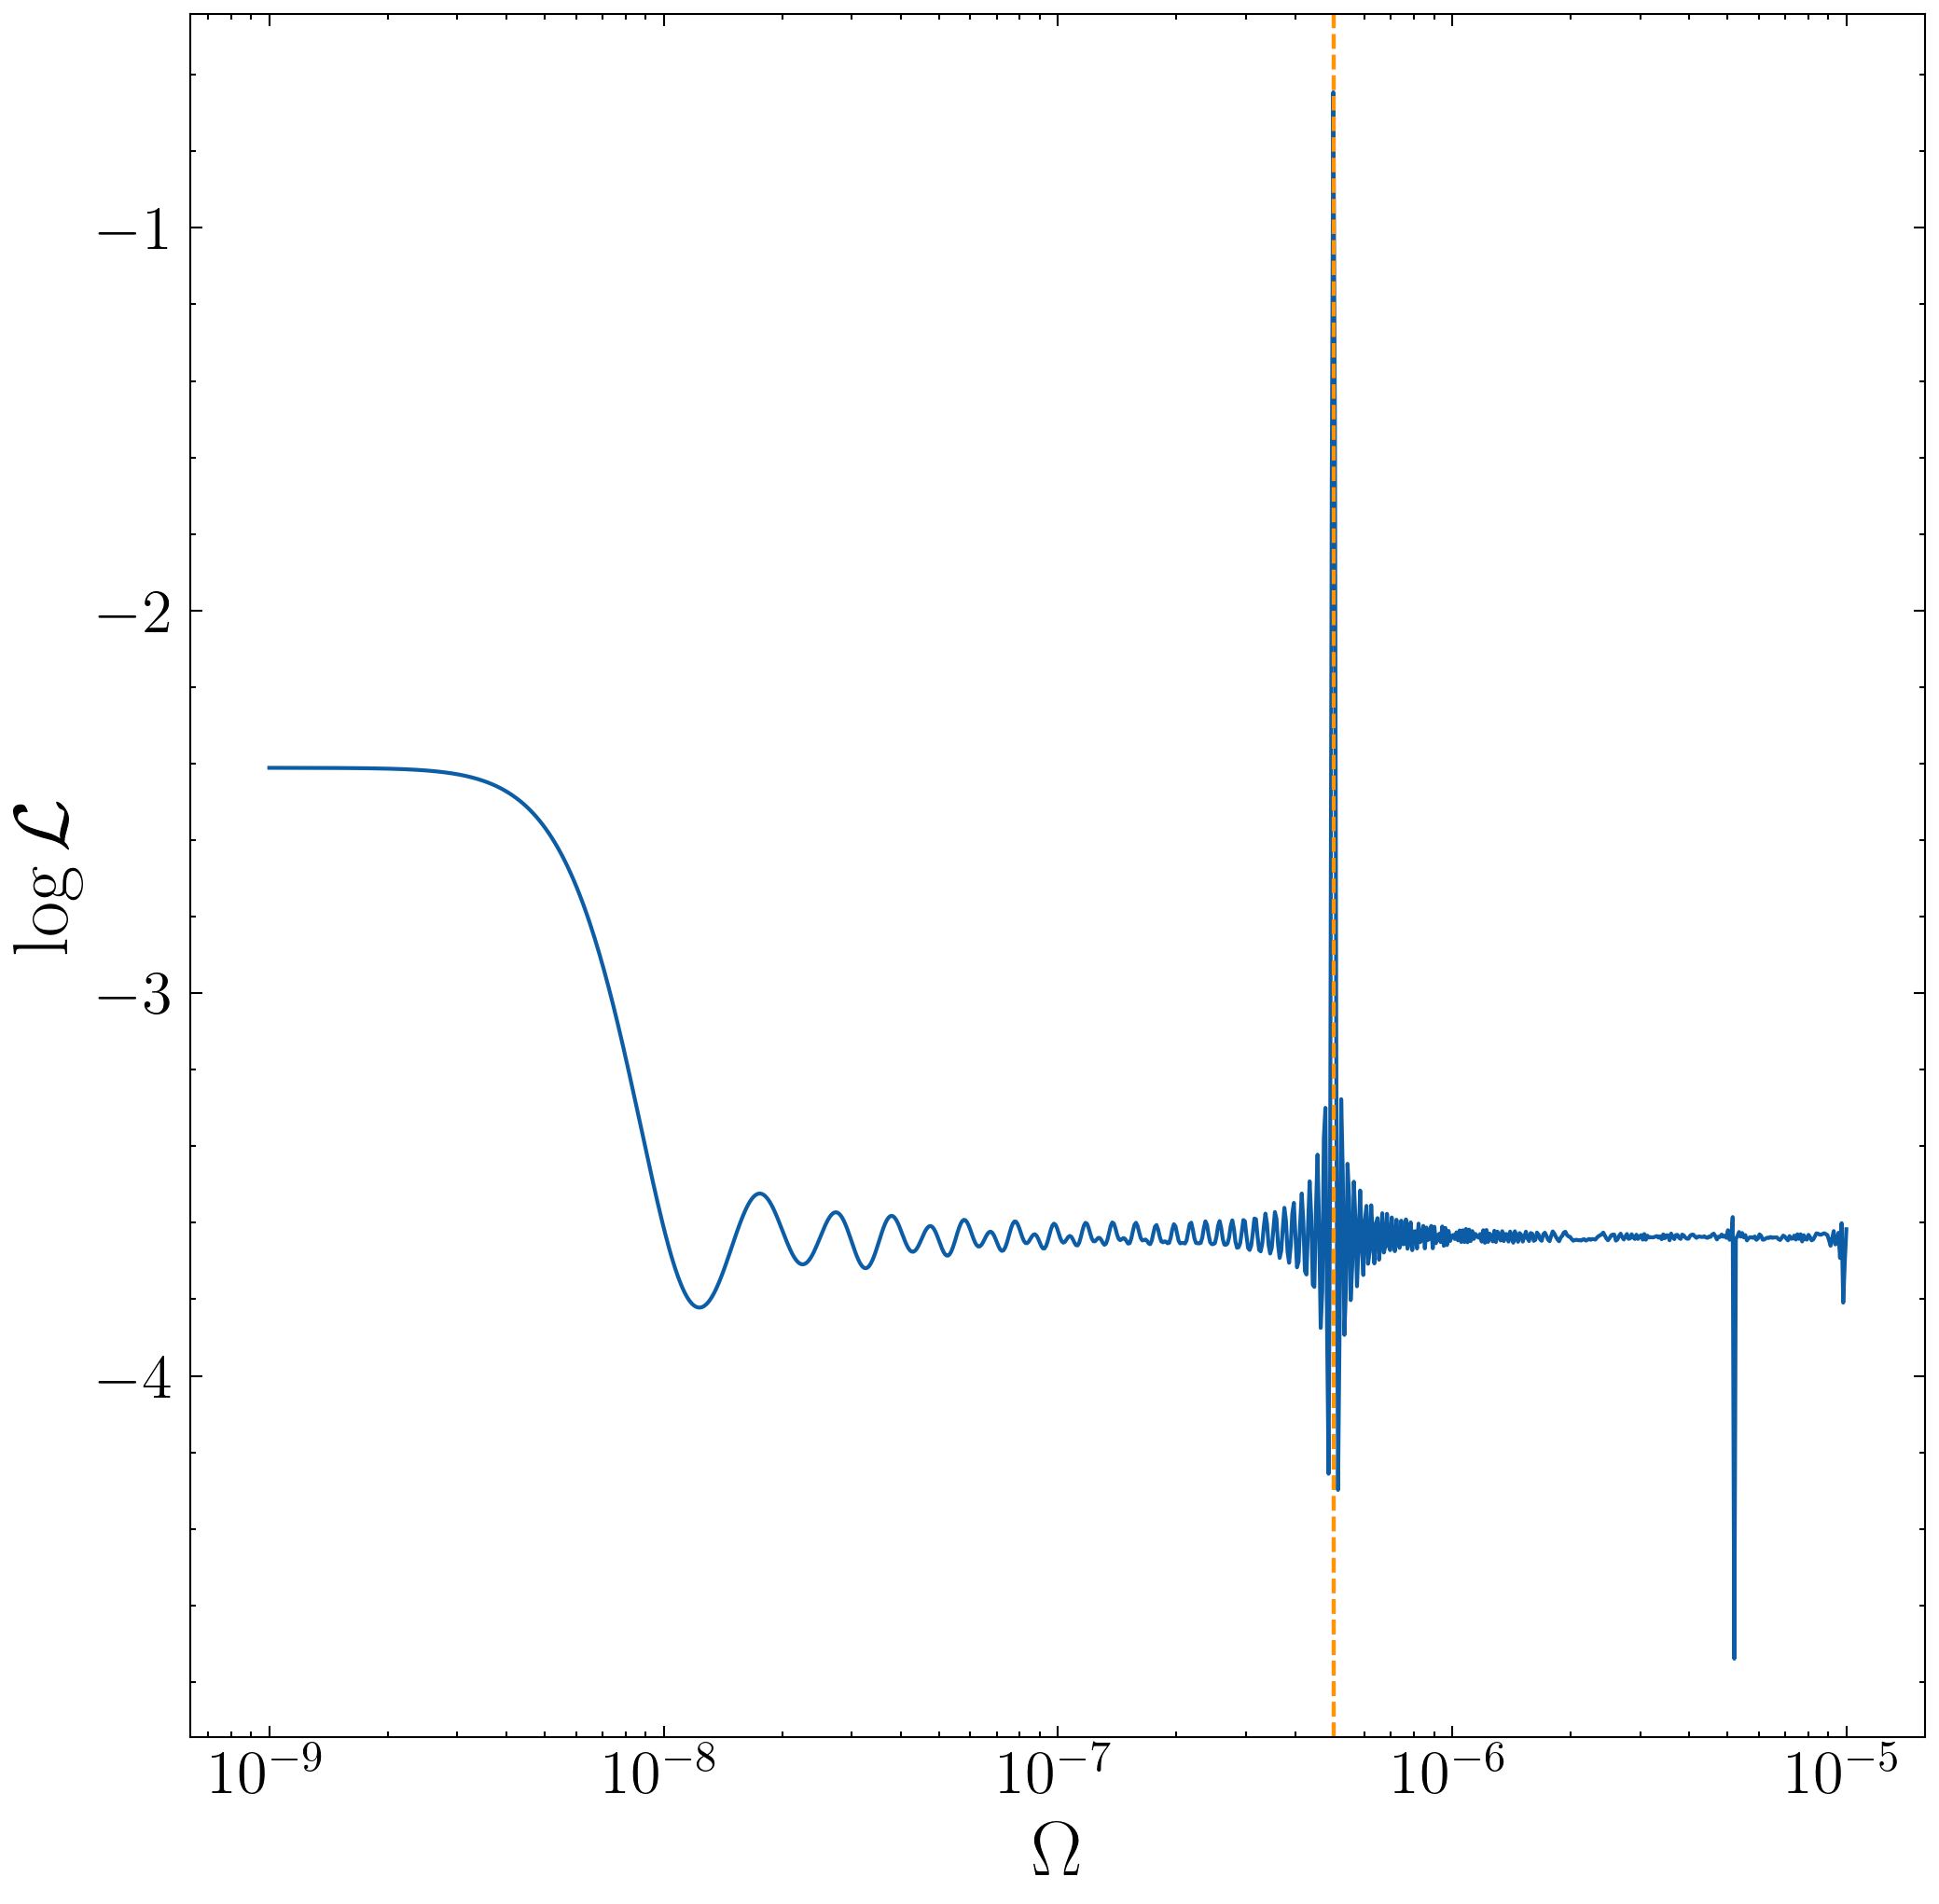
\includegraphics[width=\textwidth]{images/likelihood_omega_earth}
		\caption{$\Omega$}
		\label{fig:omega_likelihood}
	\end{subfigure}
	\hfill
	\begin{subfigure}[b]{0.22\textwidth}
		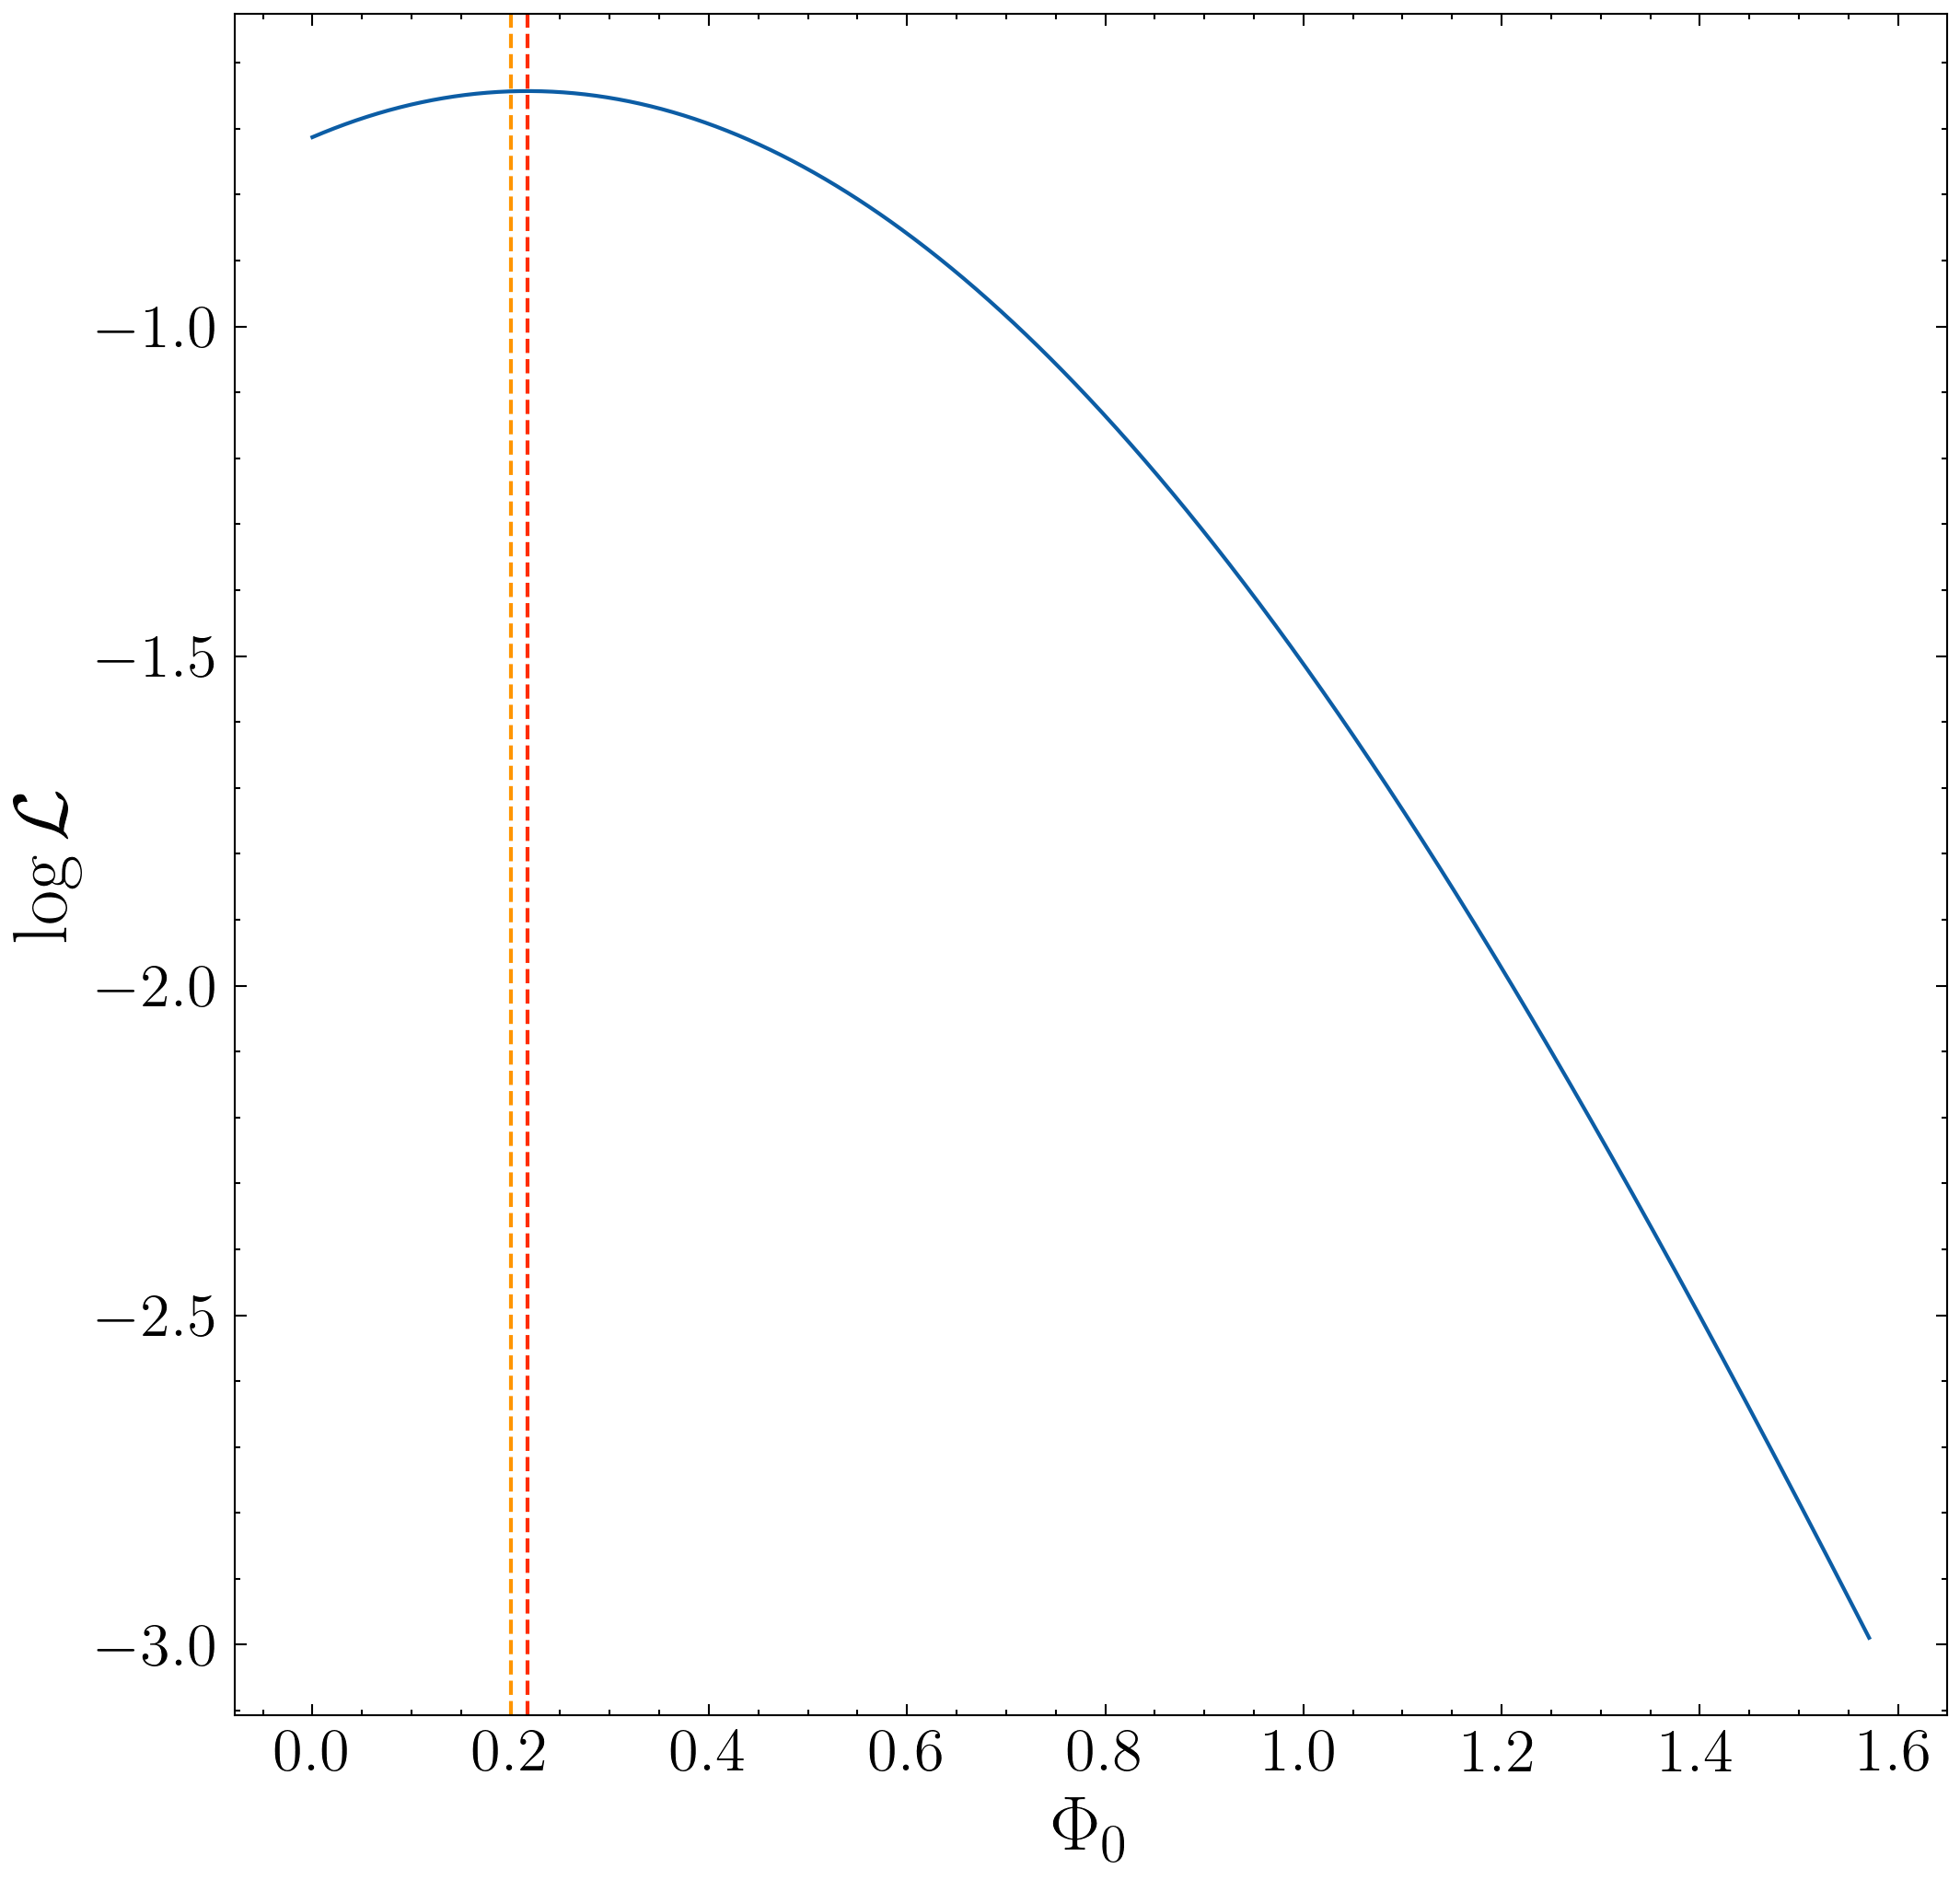
\includegraphics[width=\textwidth]{images/likelihood_phi0_earth}
		\caption{$\Phi_0$}
	\end{subfigure}
	\hfill	
	\begin{subfigure}[b]{0.22\textwidth}
		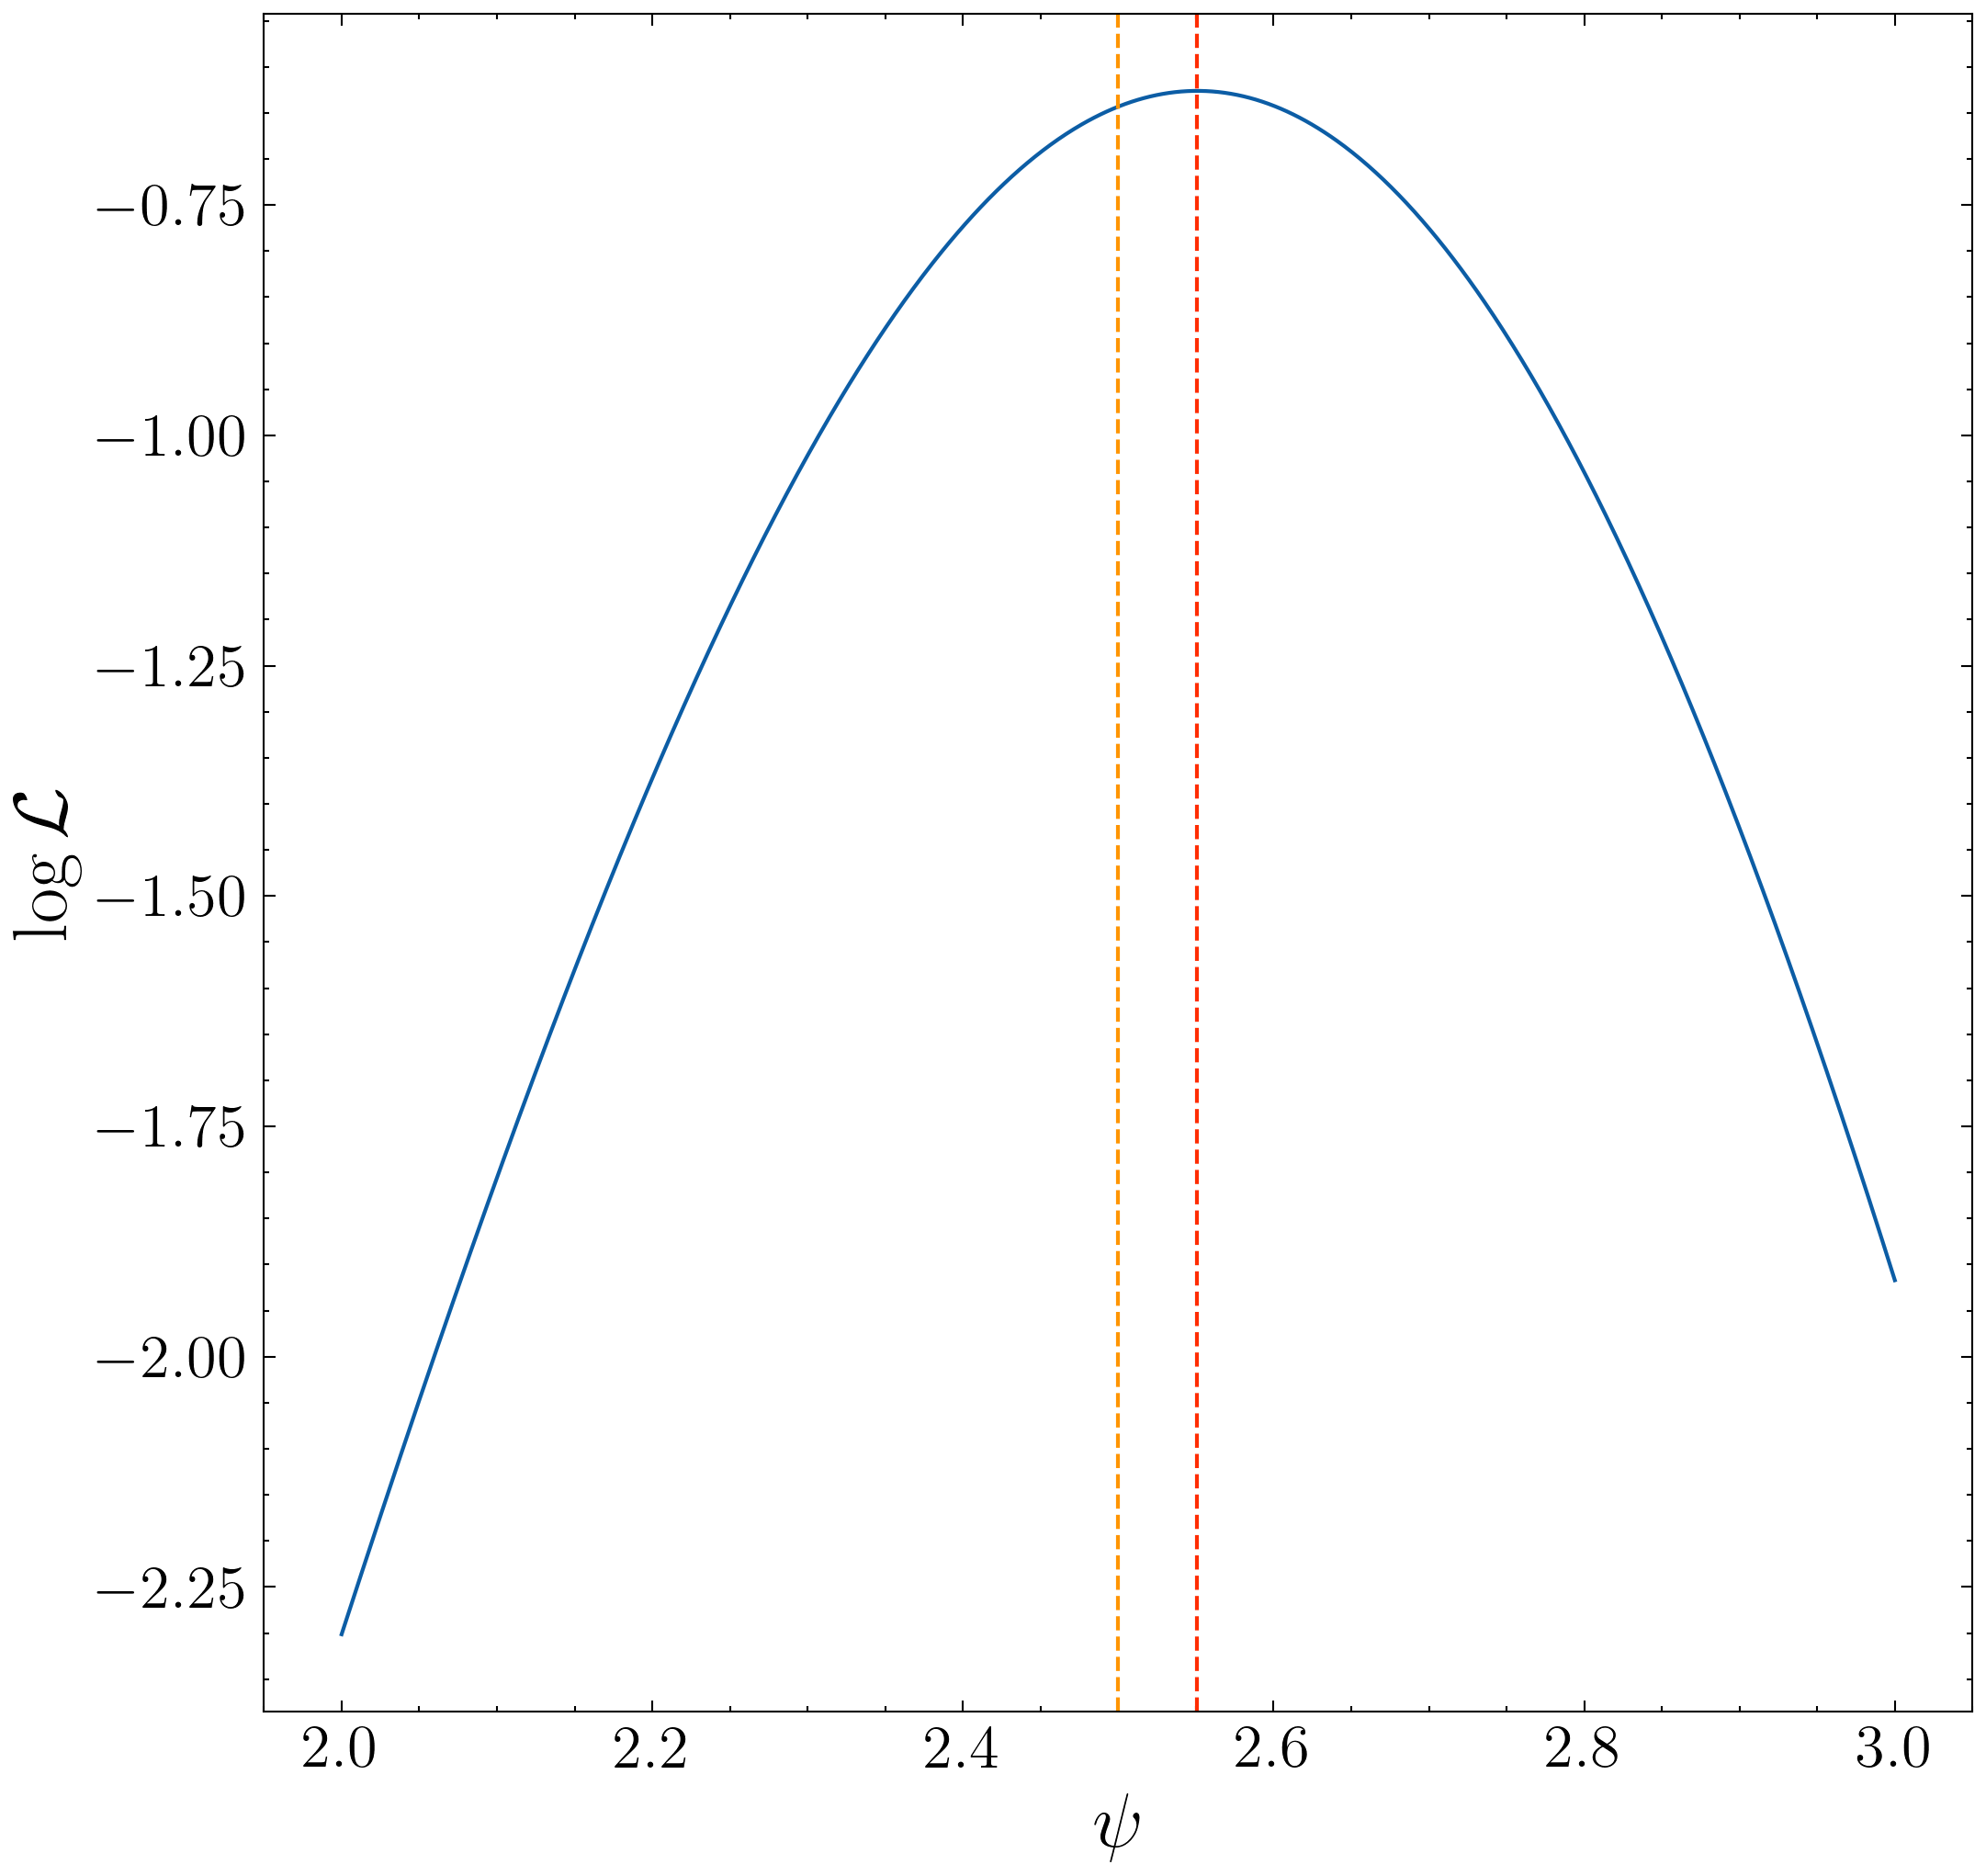
\includegraphics[width=\textwidth]{images/likelihood_psi_earth}
		\caption{$\psi$}
	\end{subfigure}
	\begin{subfigure}[b]{0.22\textwidth}
		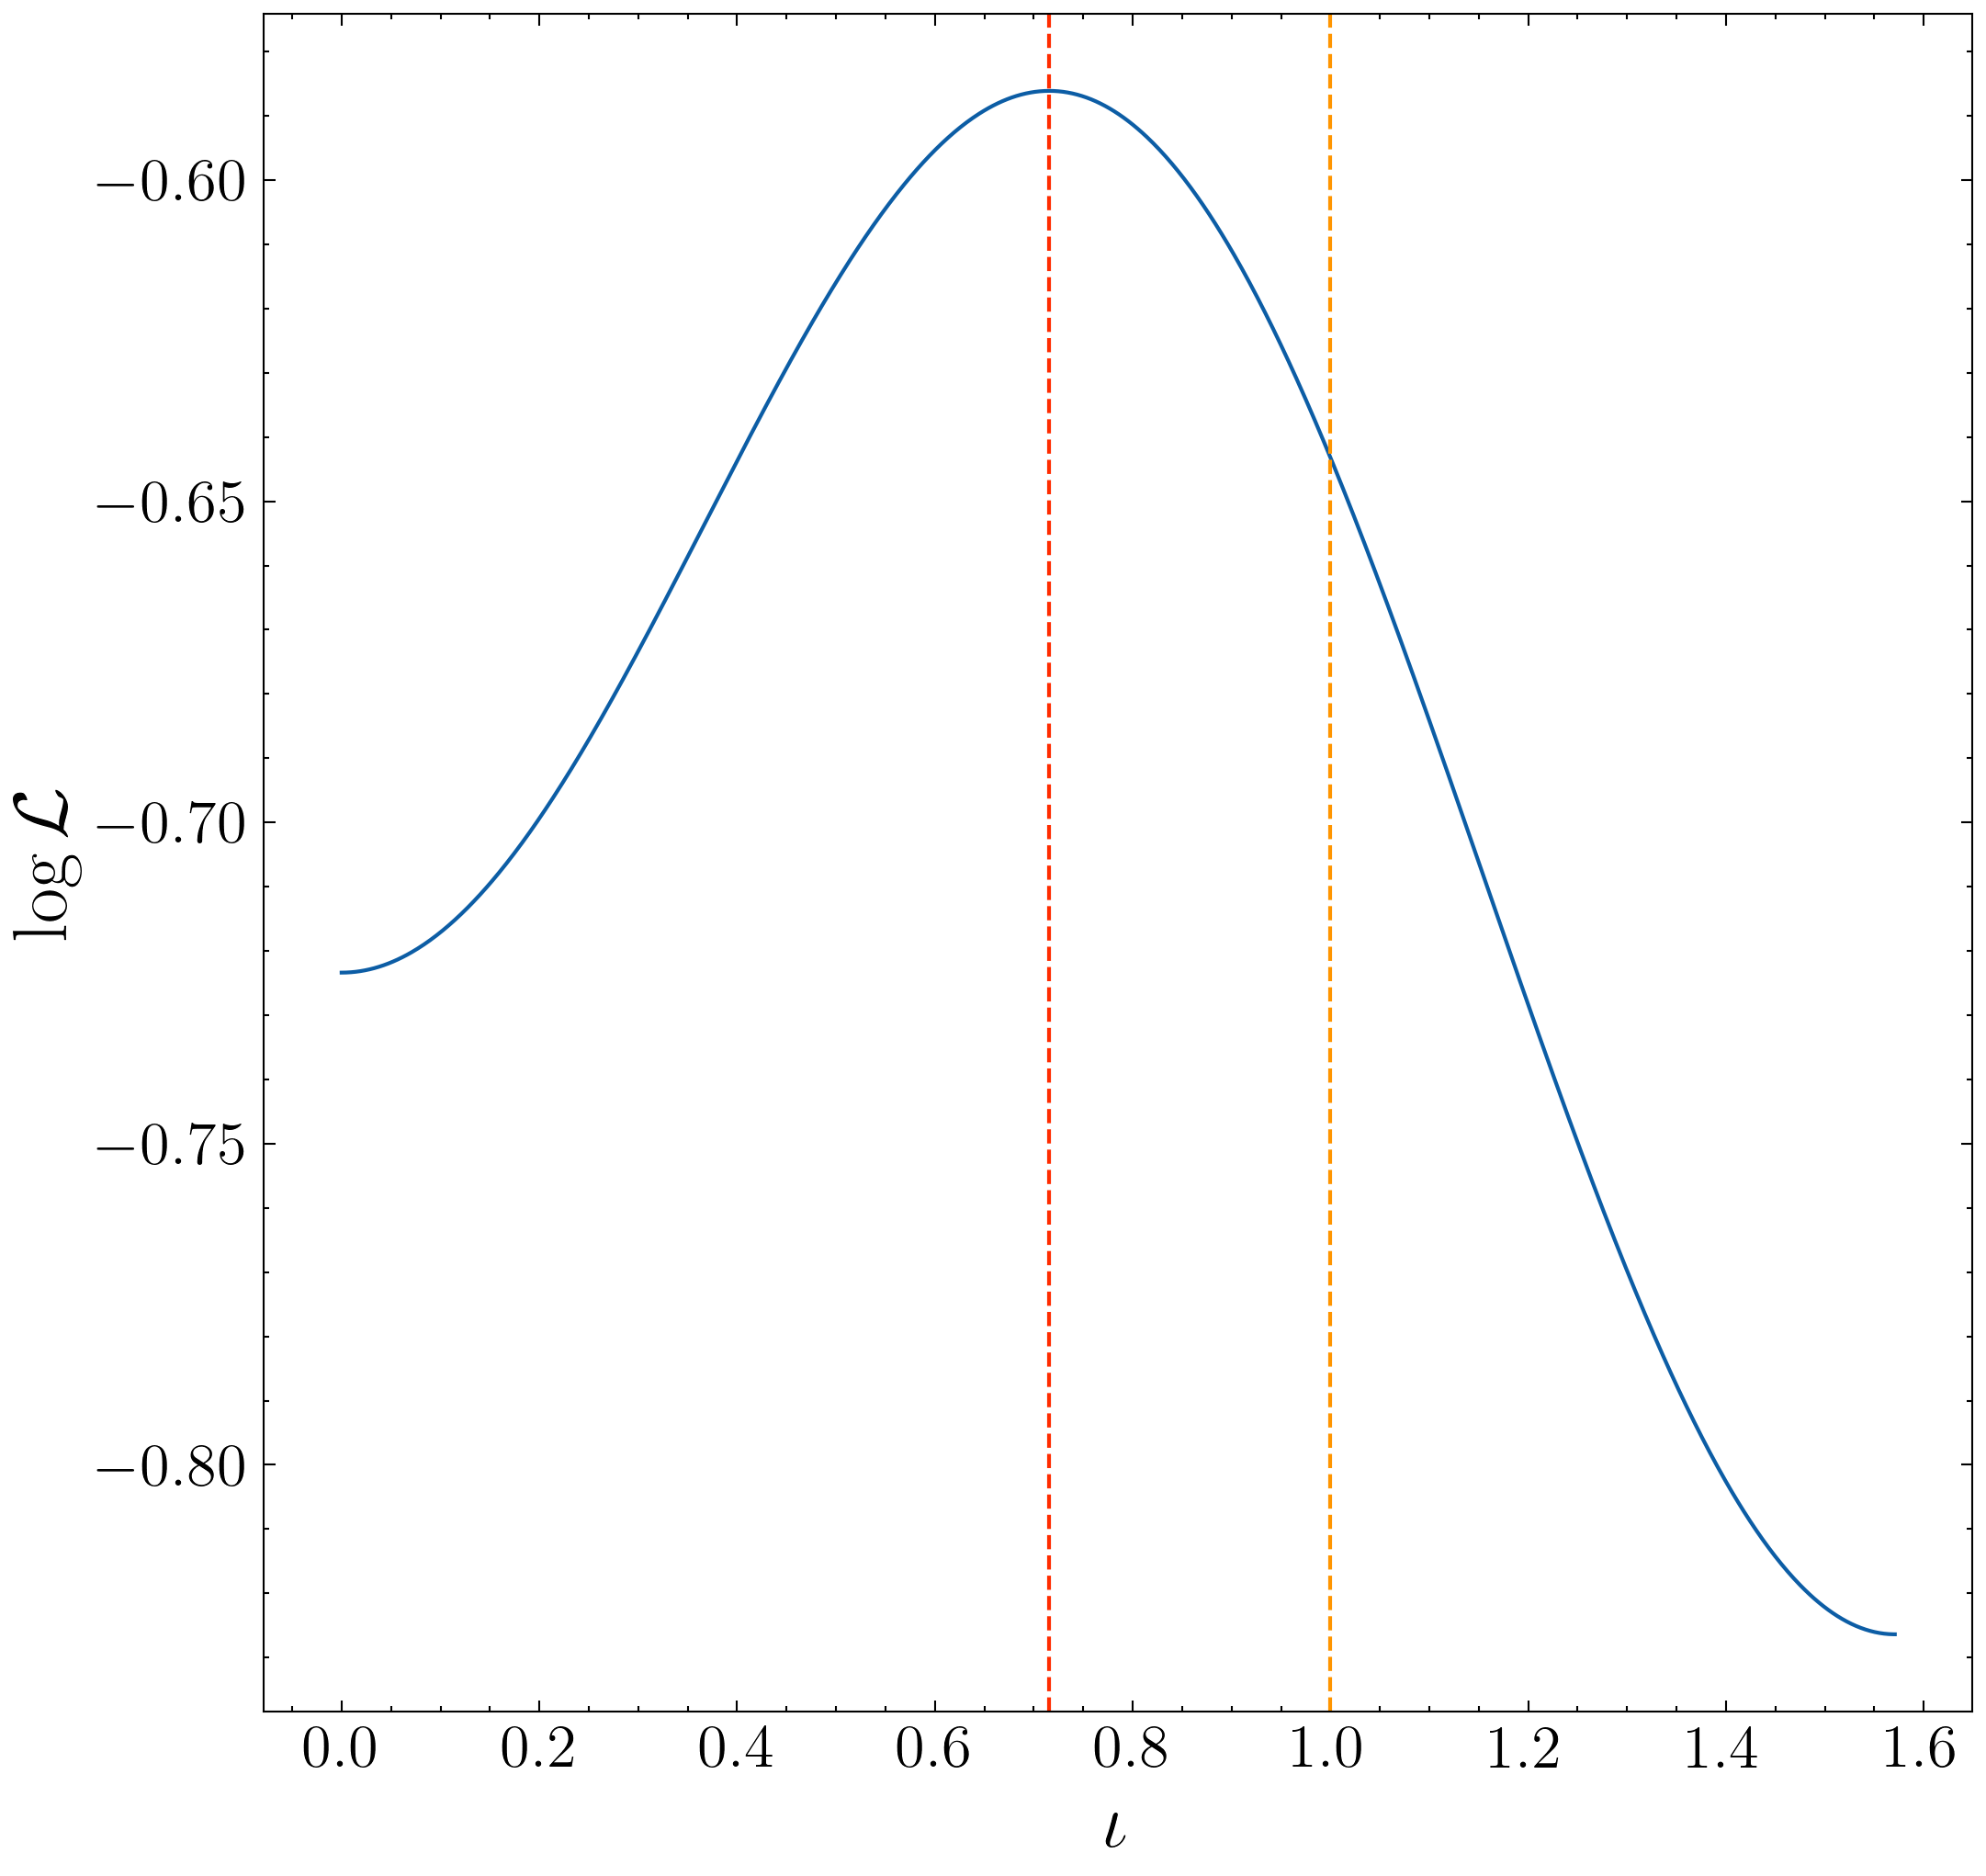
\includegraphics[width=\textwidth]{images/likelihood_iota_earth}
		\caption{$\iota$}
			\label{fig:iota_likelihood}
	\end{subfigure}
	\medskip
	\begin{subfigure}[b]{0.3\textwidth}
		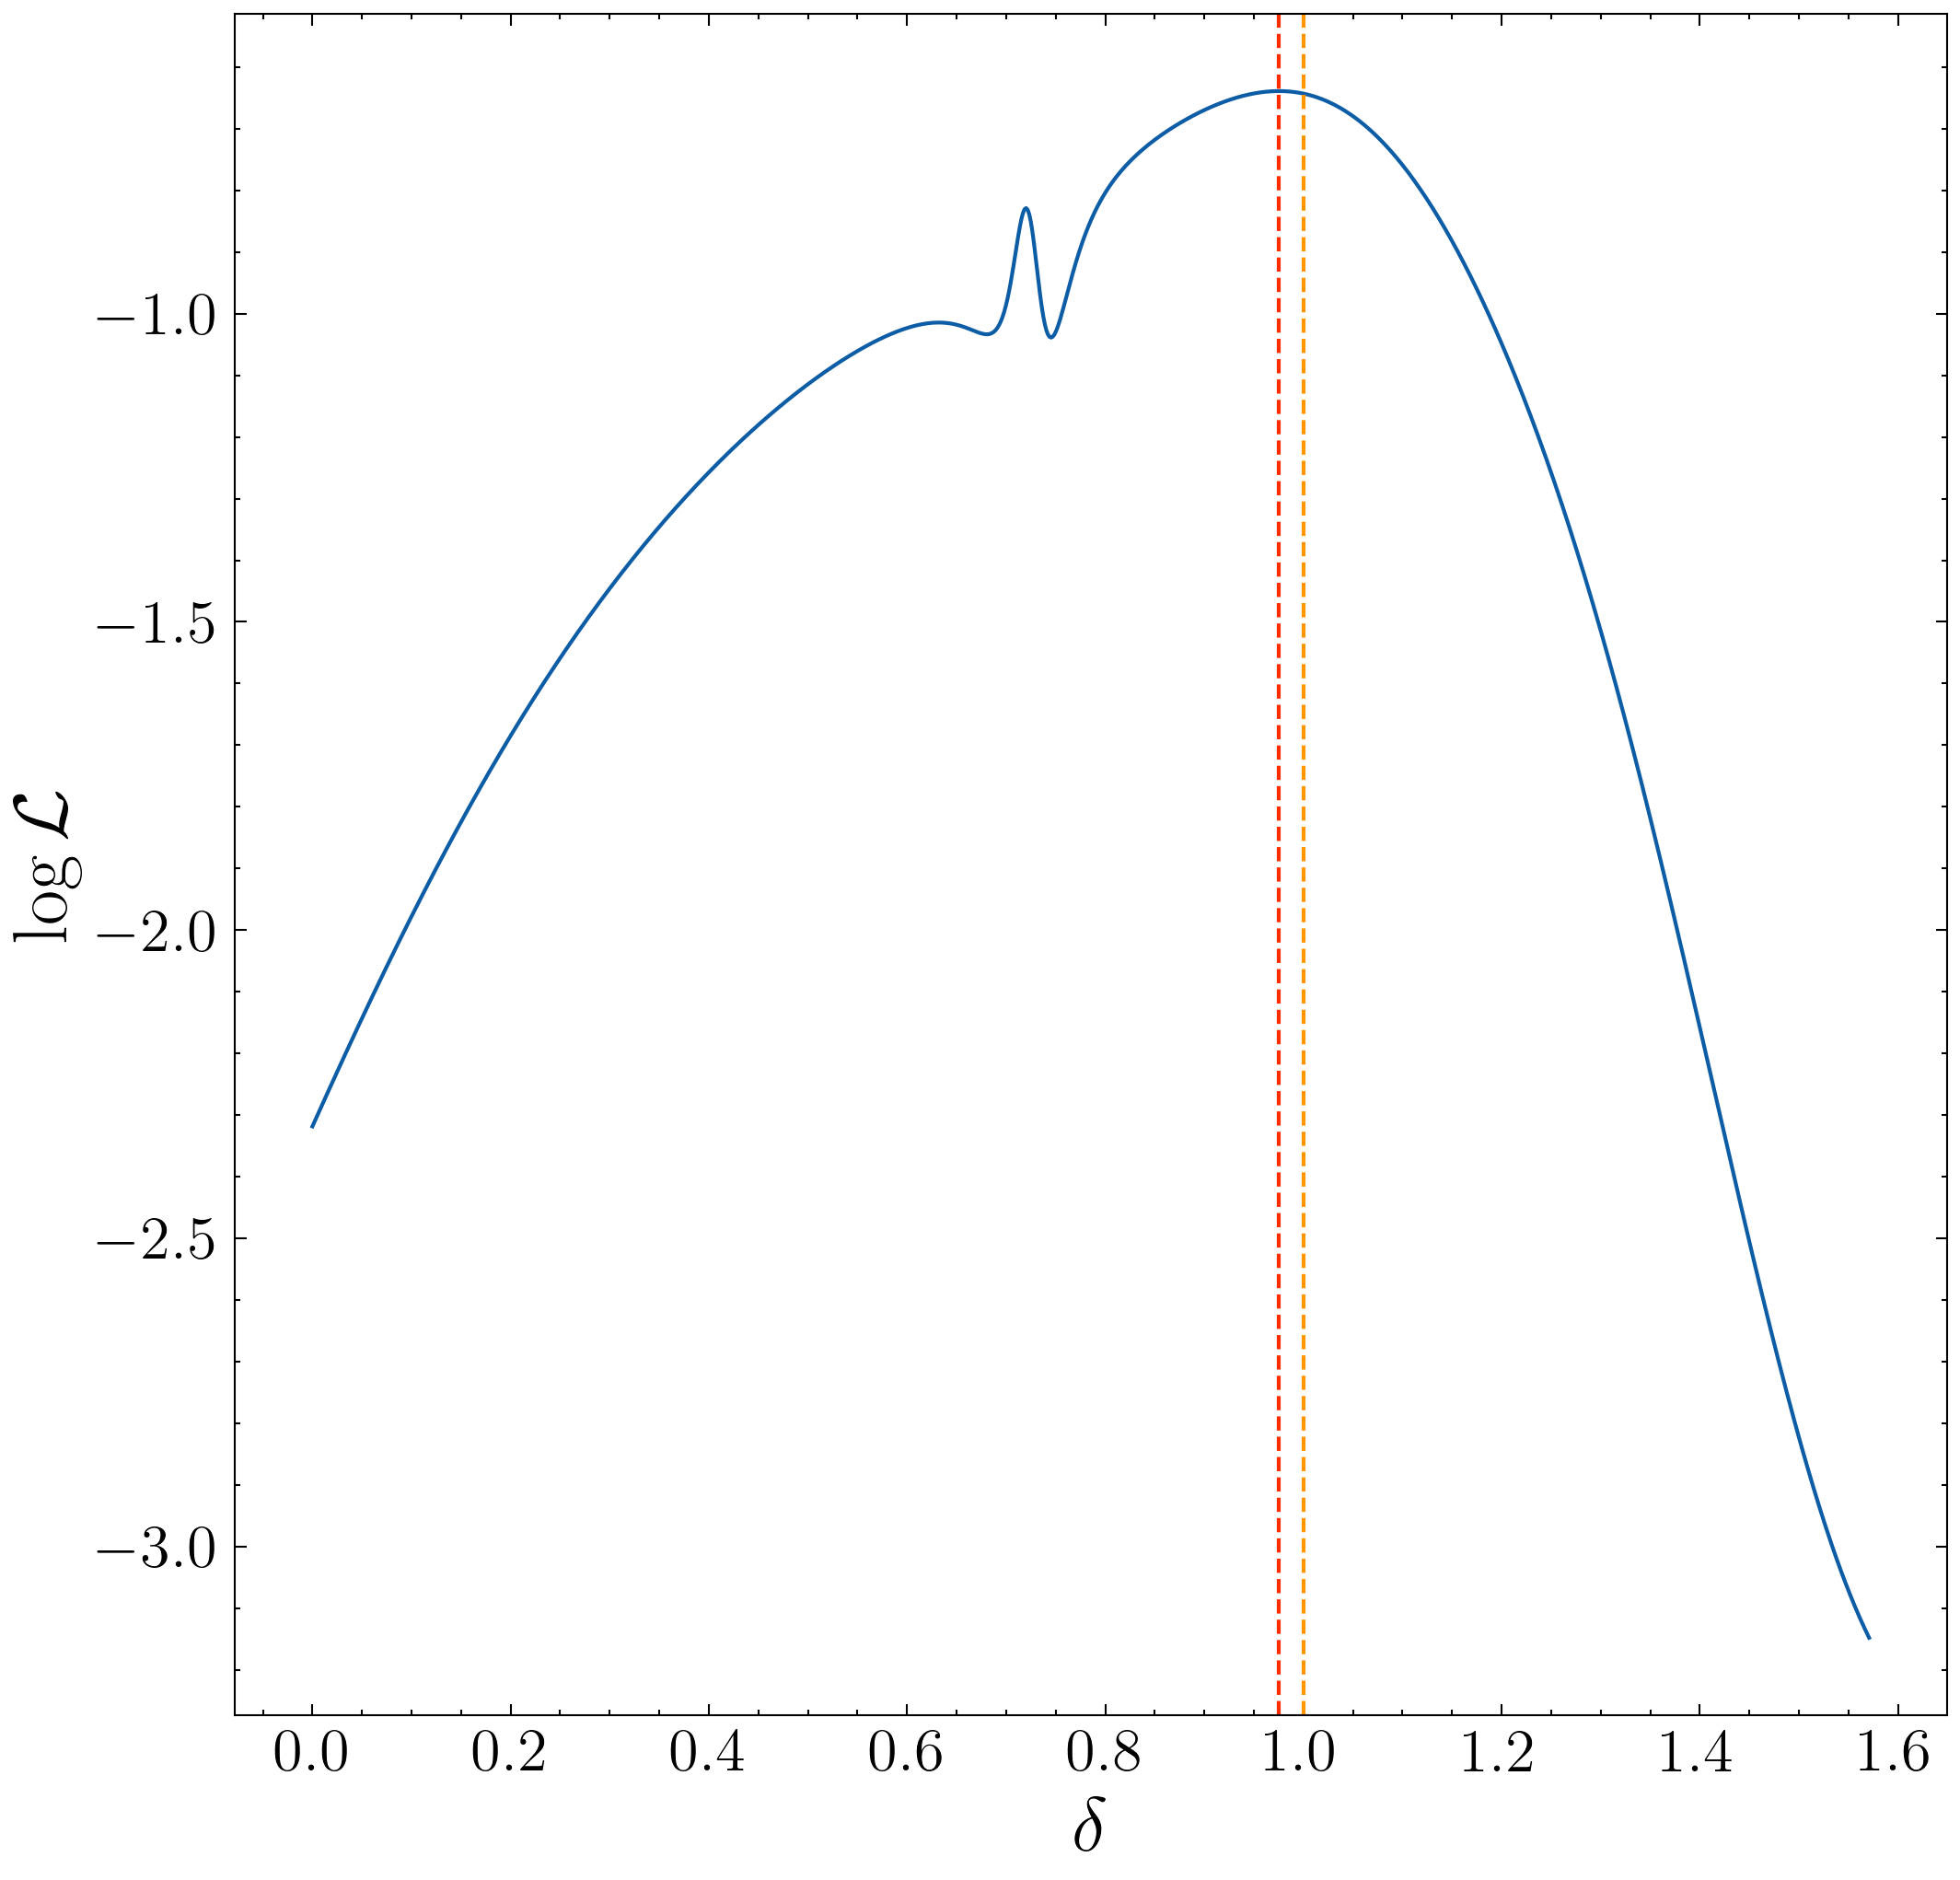
\includegraphics[width=\textwidth]{images/likelihood_delta_earth}
		\caption{$\delta$}
	\end{subfigure}
	\hfill
	\begin{subfigure}[b]{0.3\textwidth}
		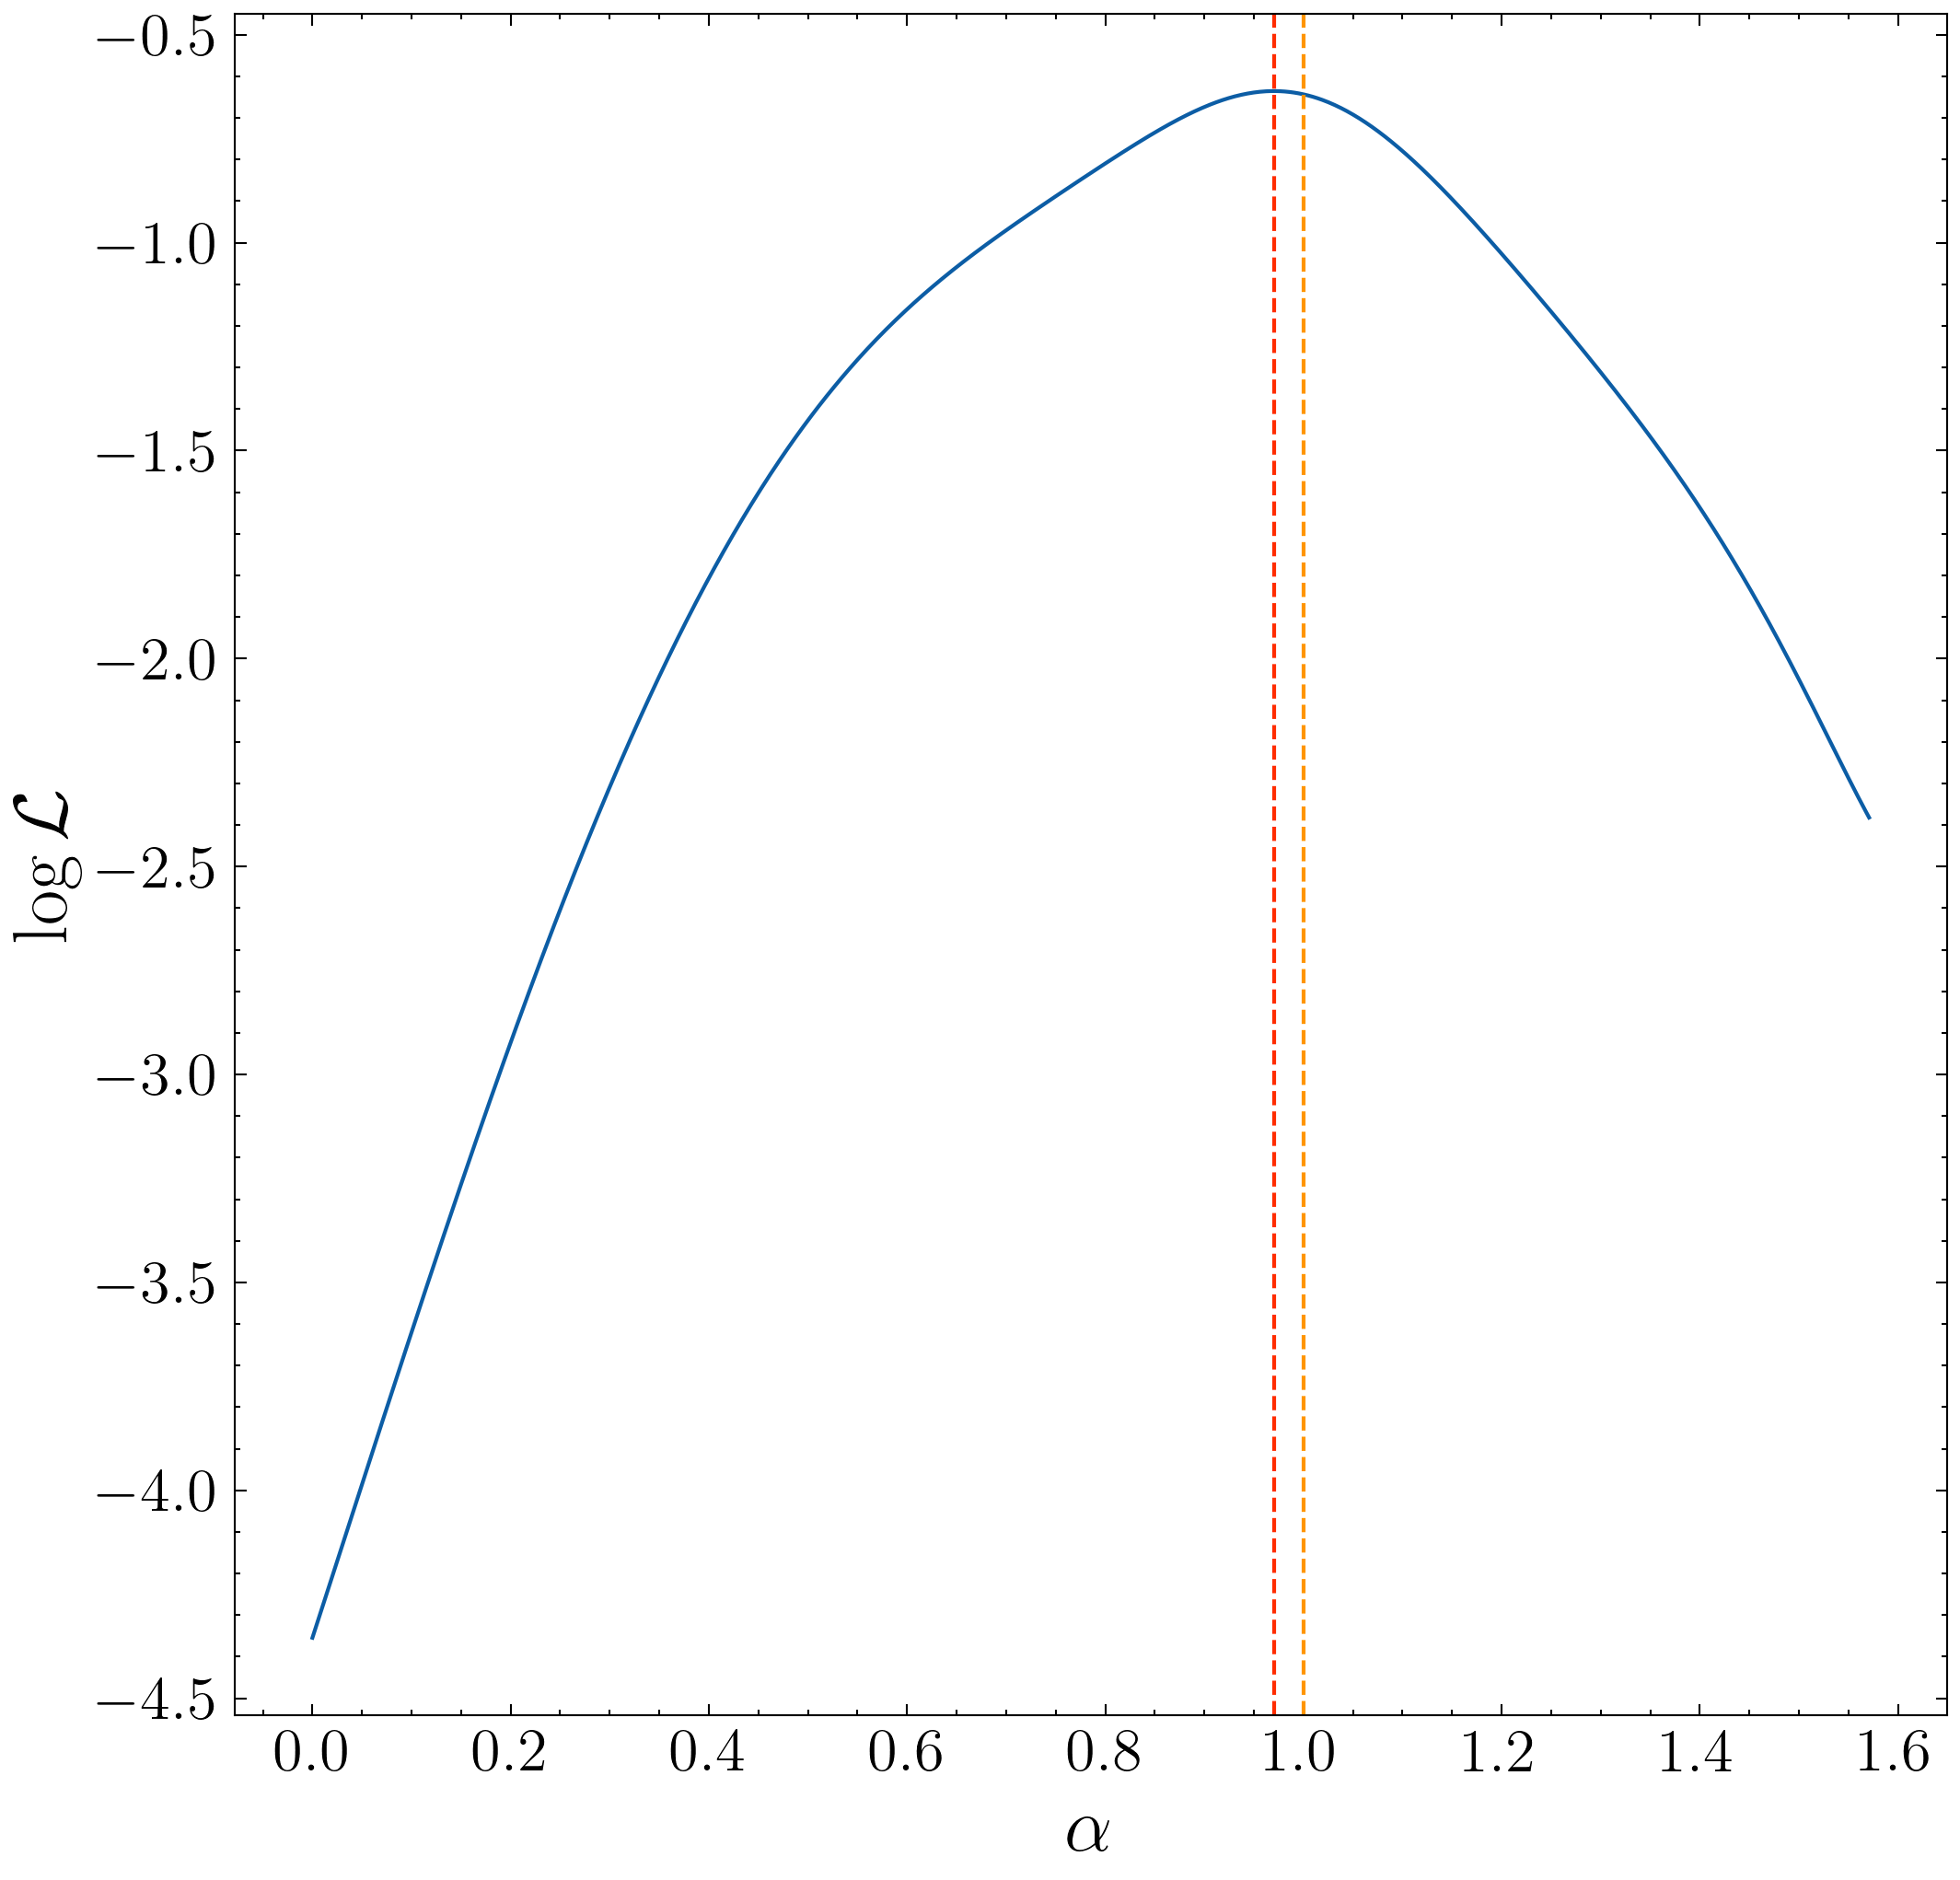
\includegraphics[width=\textwidth]{images/likelihood_alpha_earth}
		\caption{$\alpha$}
	\end{subfigure}
	\hfill
	\begin{subfigure}[b]{0.3\textwidth}
		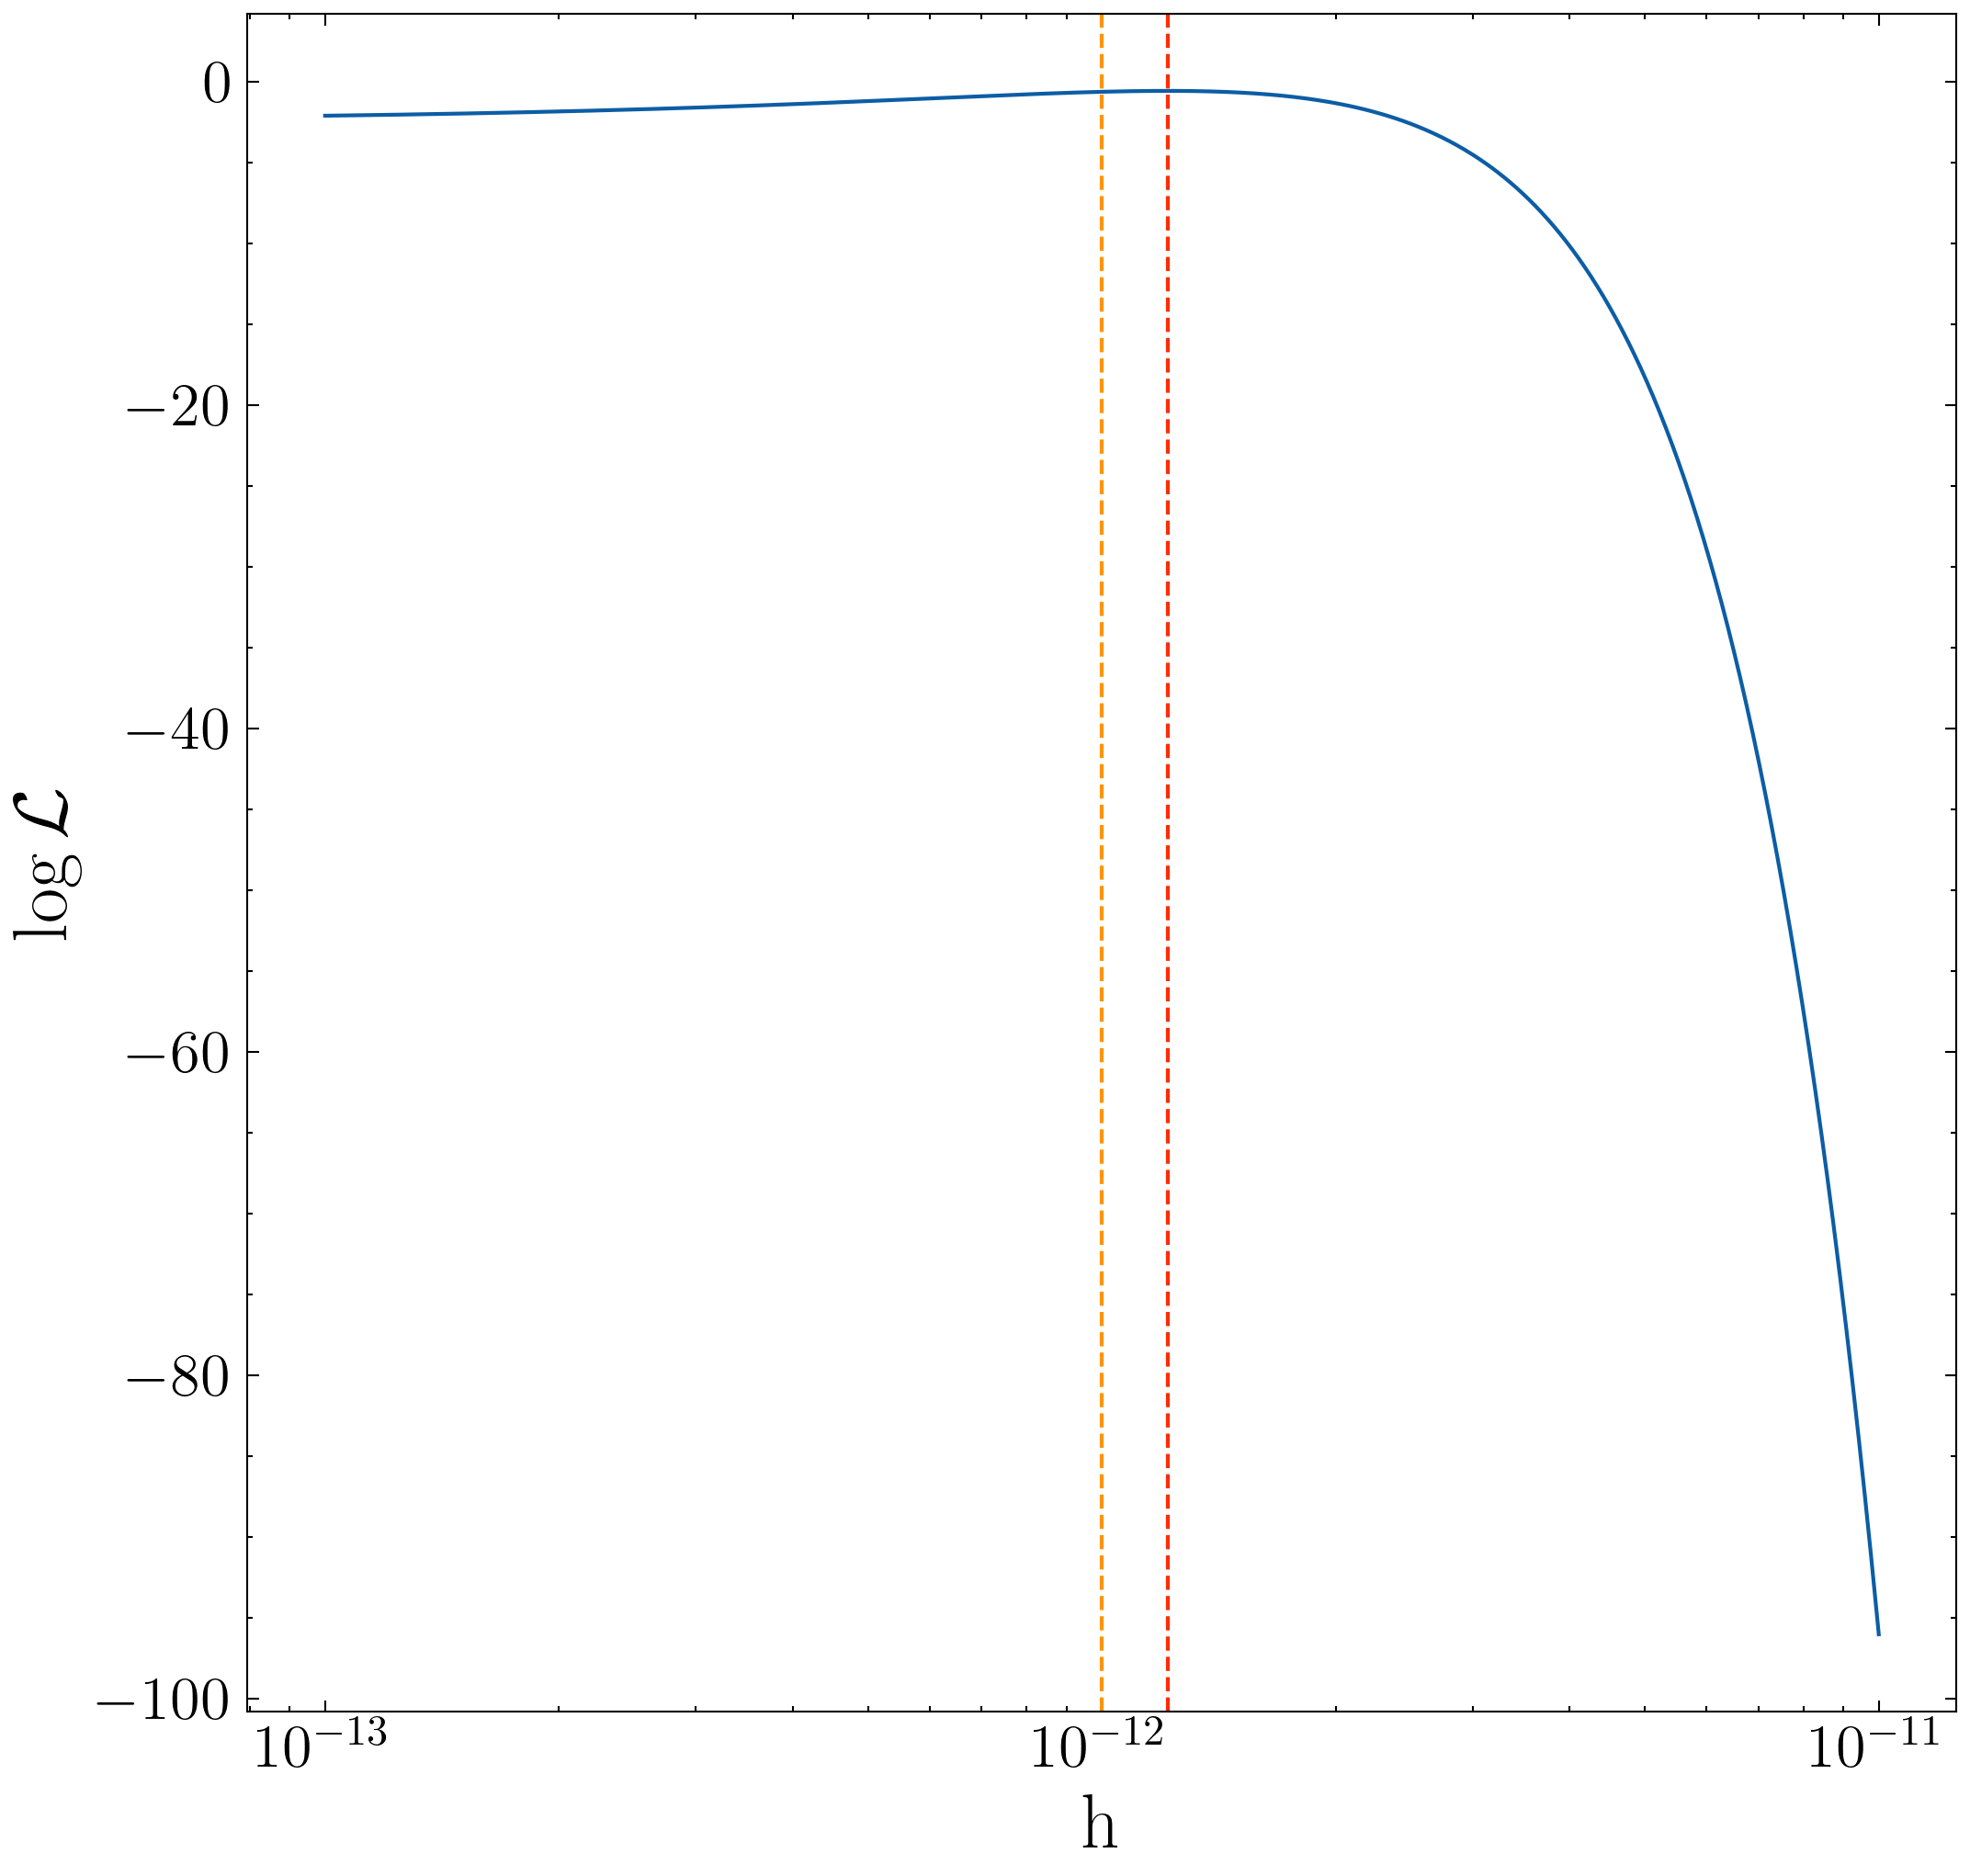
\includegraphics{images/likelihood_h_earth}
		\caption{$h$}
	\end{subfigure}
	
	\caption{}\label{fig:likelihood_curves_earth}
\end{figure*}








\begin{figure*}
	\setkeys{Gin}{width=\linewidth}   
	
	\begin{subfigure}[b]{0.22\textwidth}
		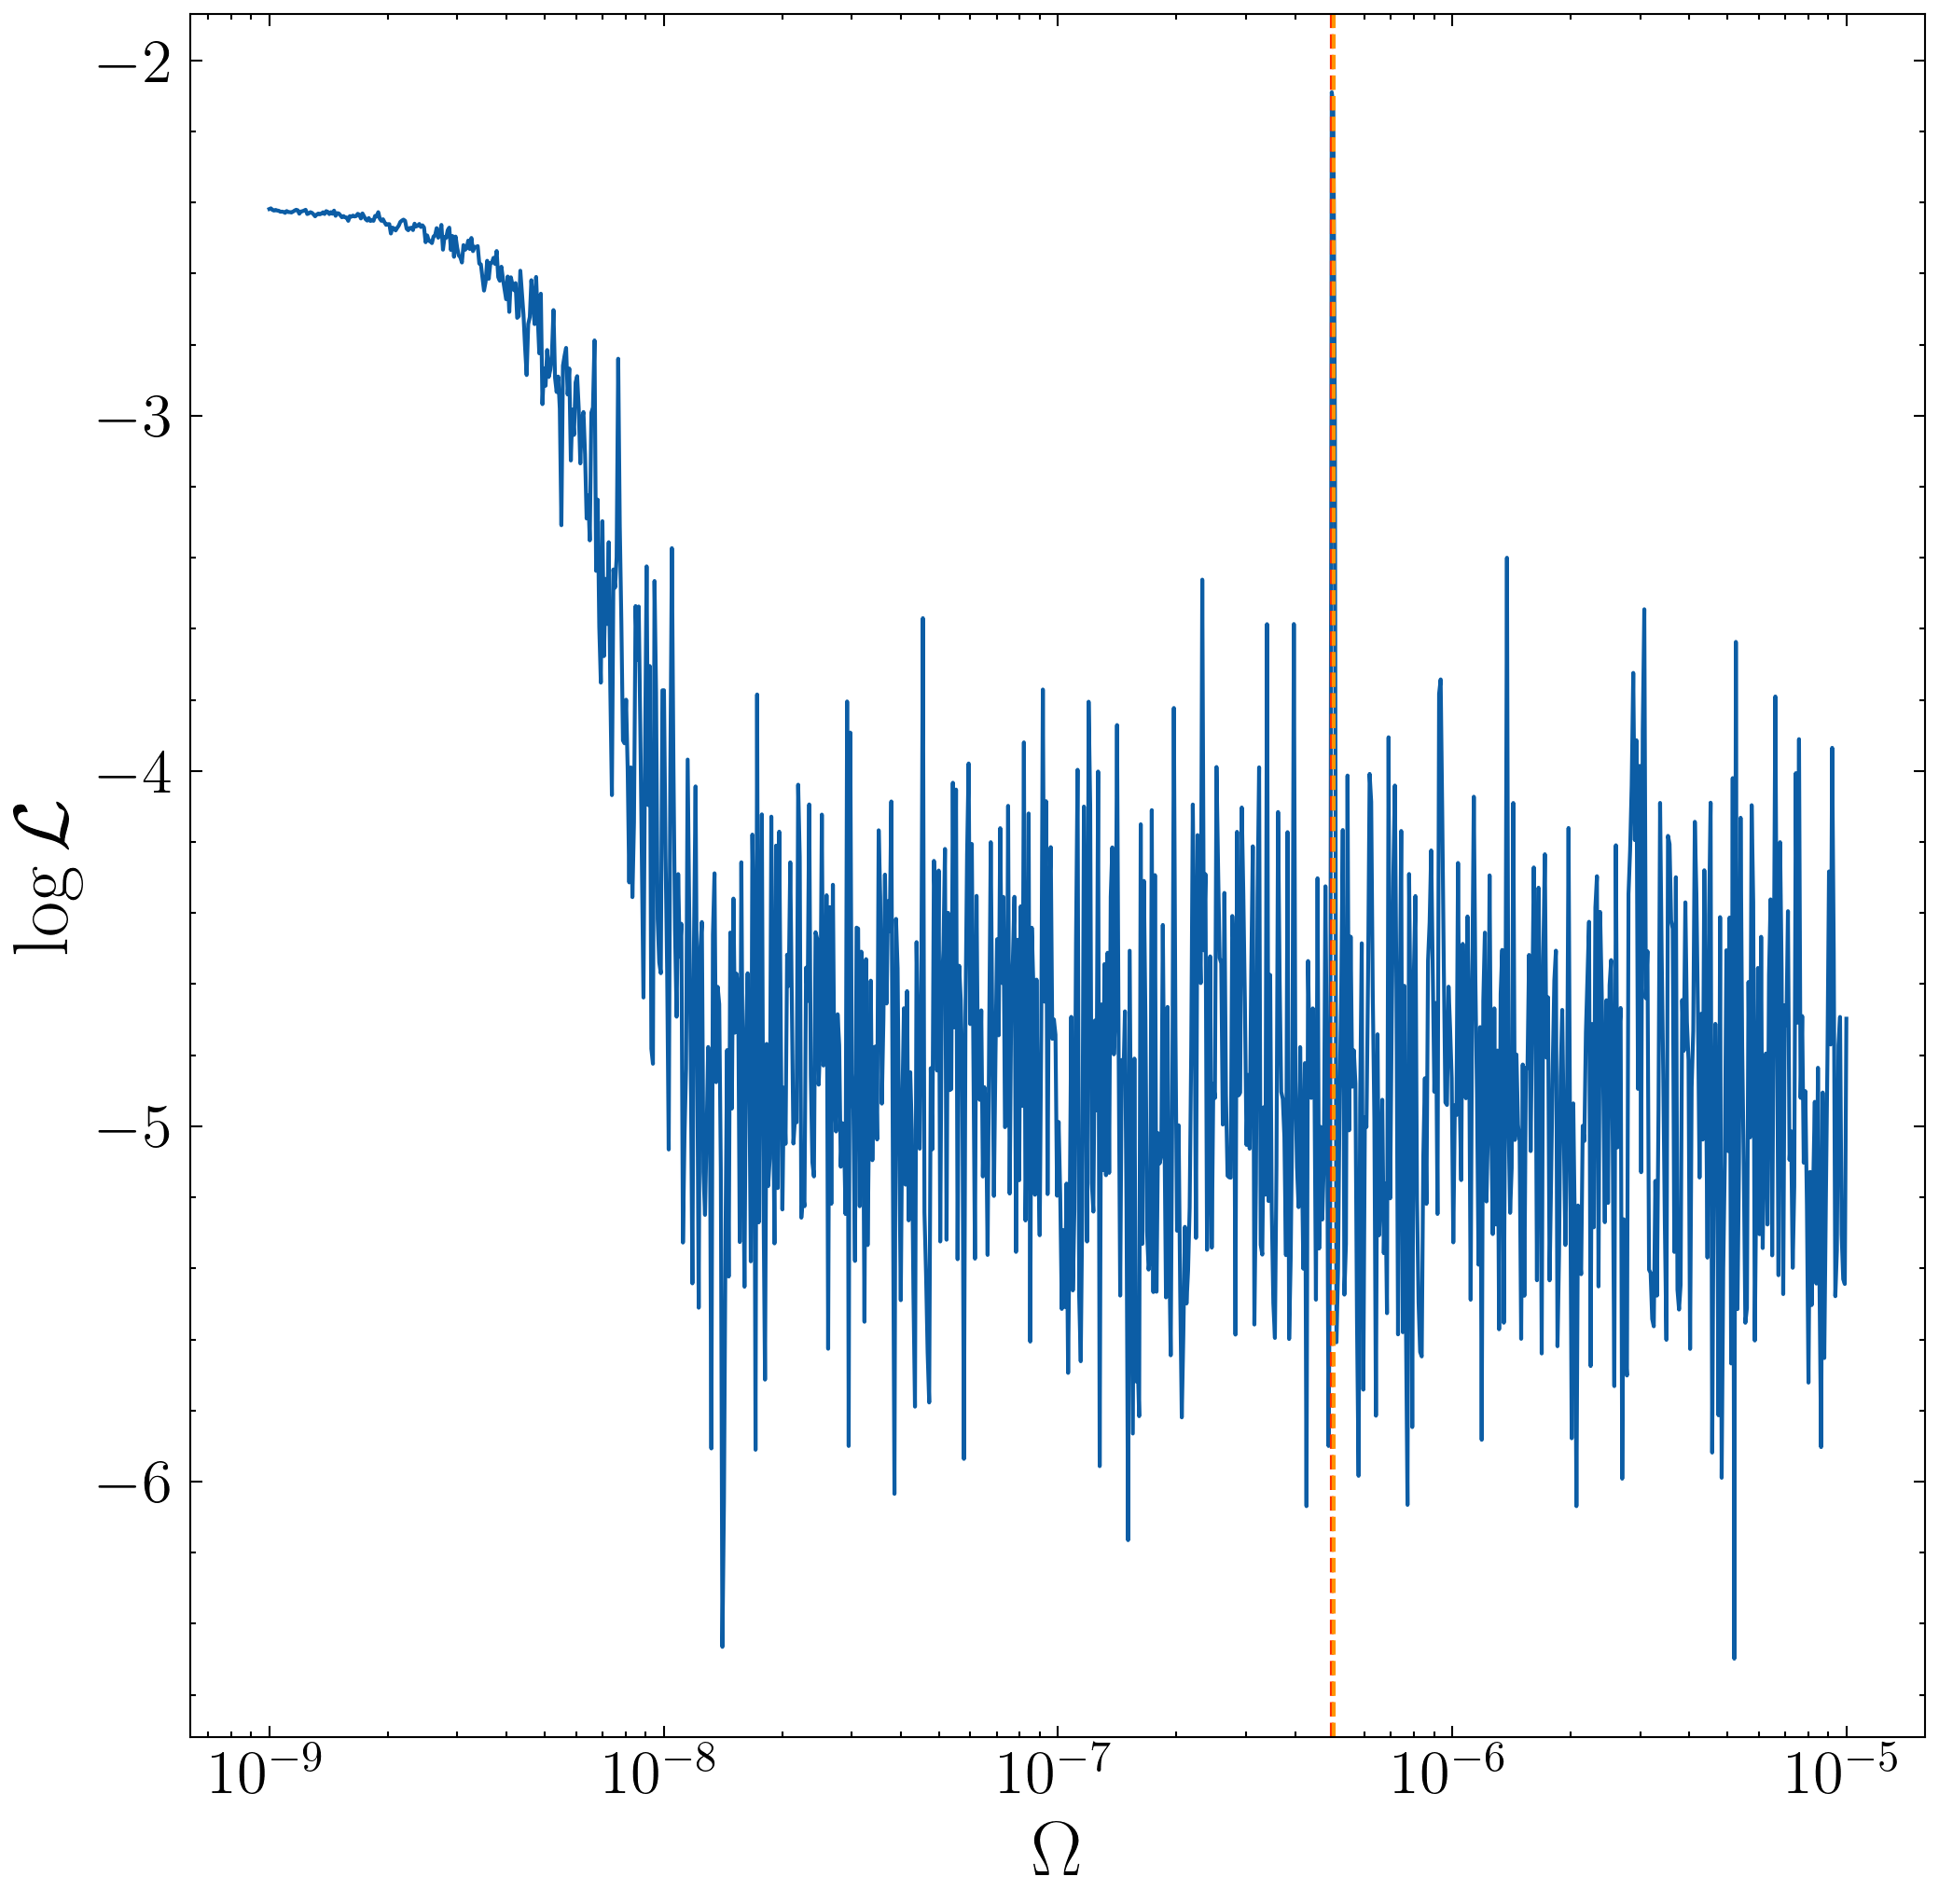
\includegraphics[width=\textwidth]{images/likelihood_omega_psr}
		\caption{$\Omega$}
	\end{subfigure}
	\hfill
	\begin{subfigure}[b]{0.22\textwidth}
		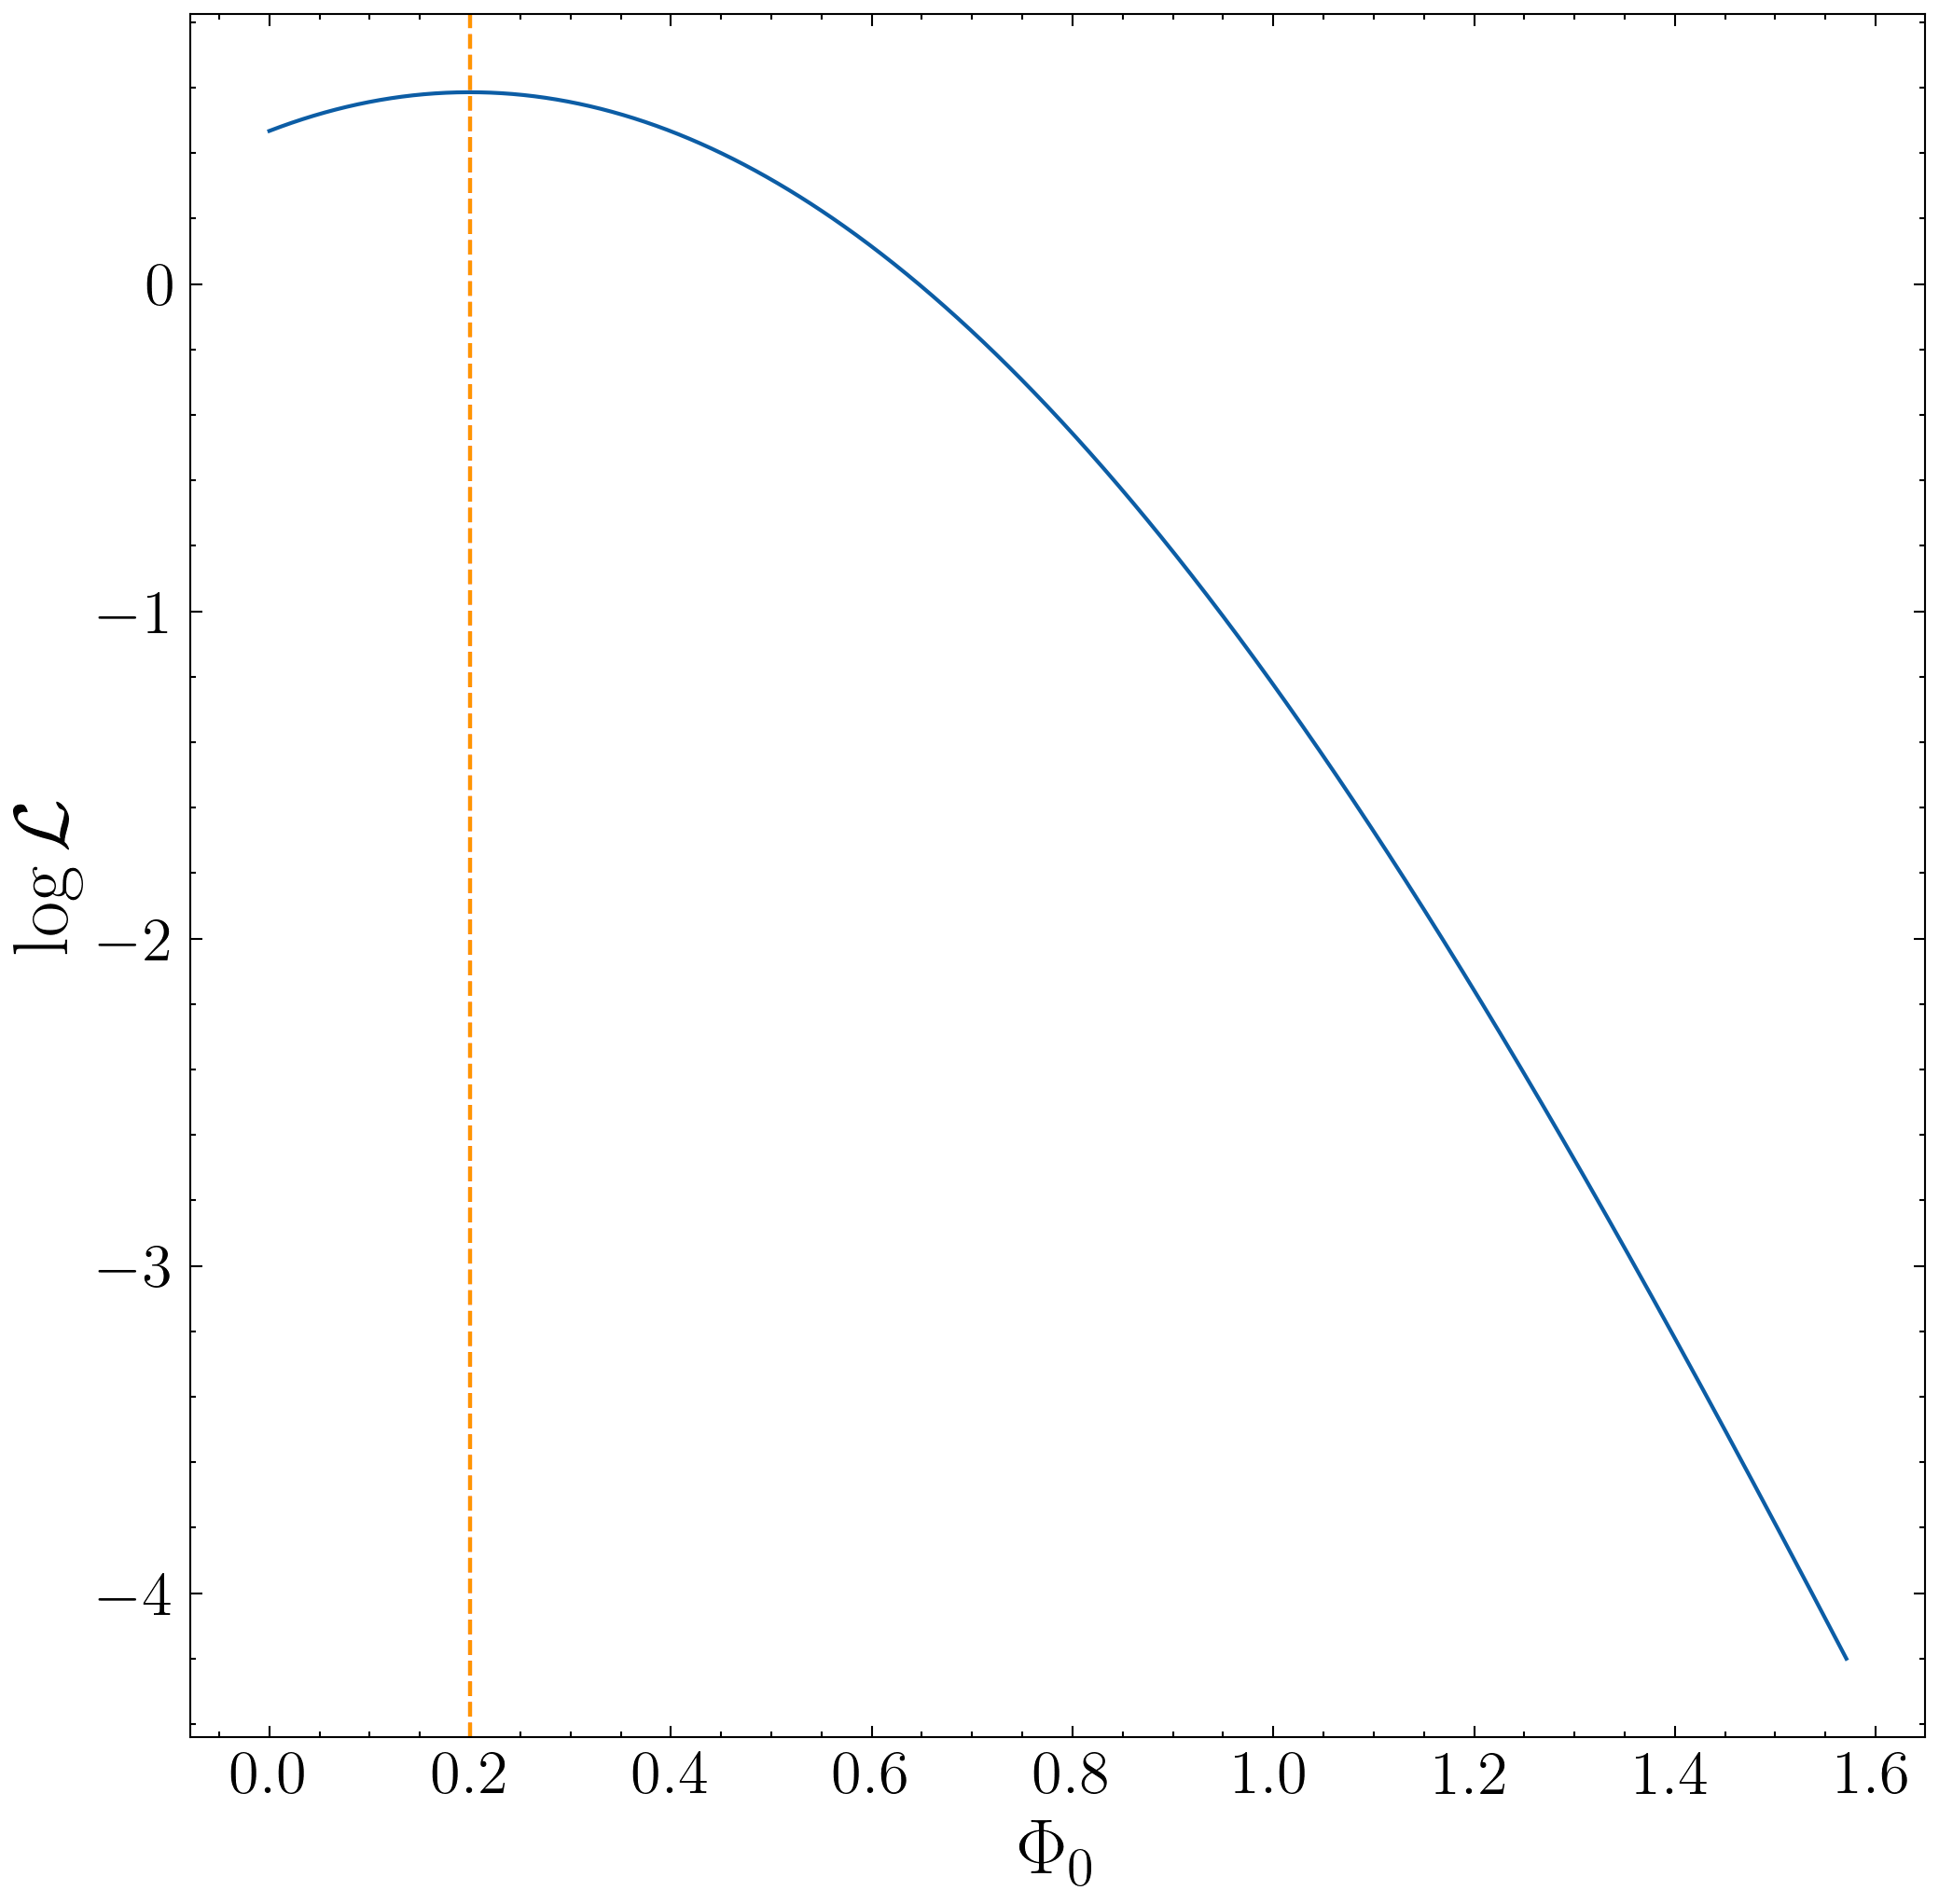
\includegraphics[width=\textwidth]{images/likelihood_phi0_psr}
		\caption{$\Phi_0$}
	\end{subfigure}
	\hfill	
	\begin{subfigure}[b]{0.22\textwidth}
		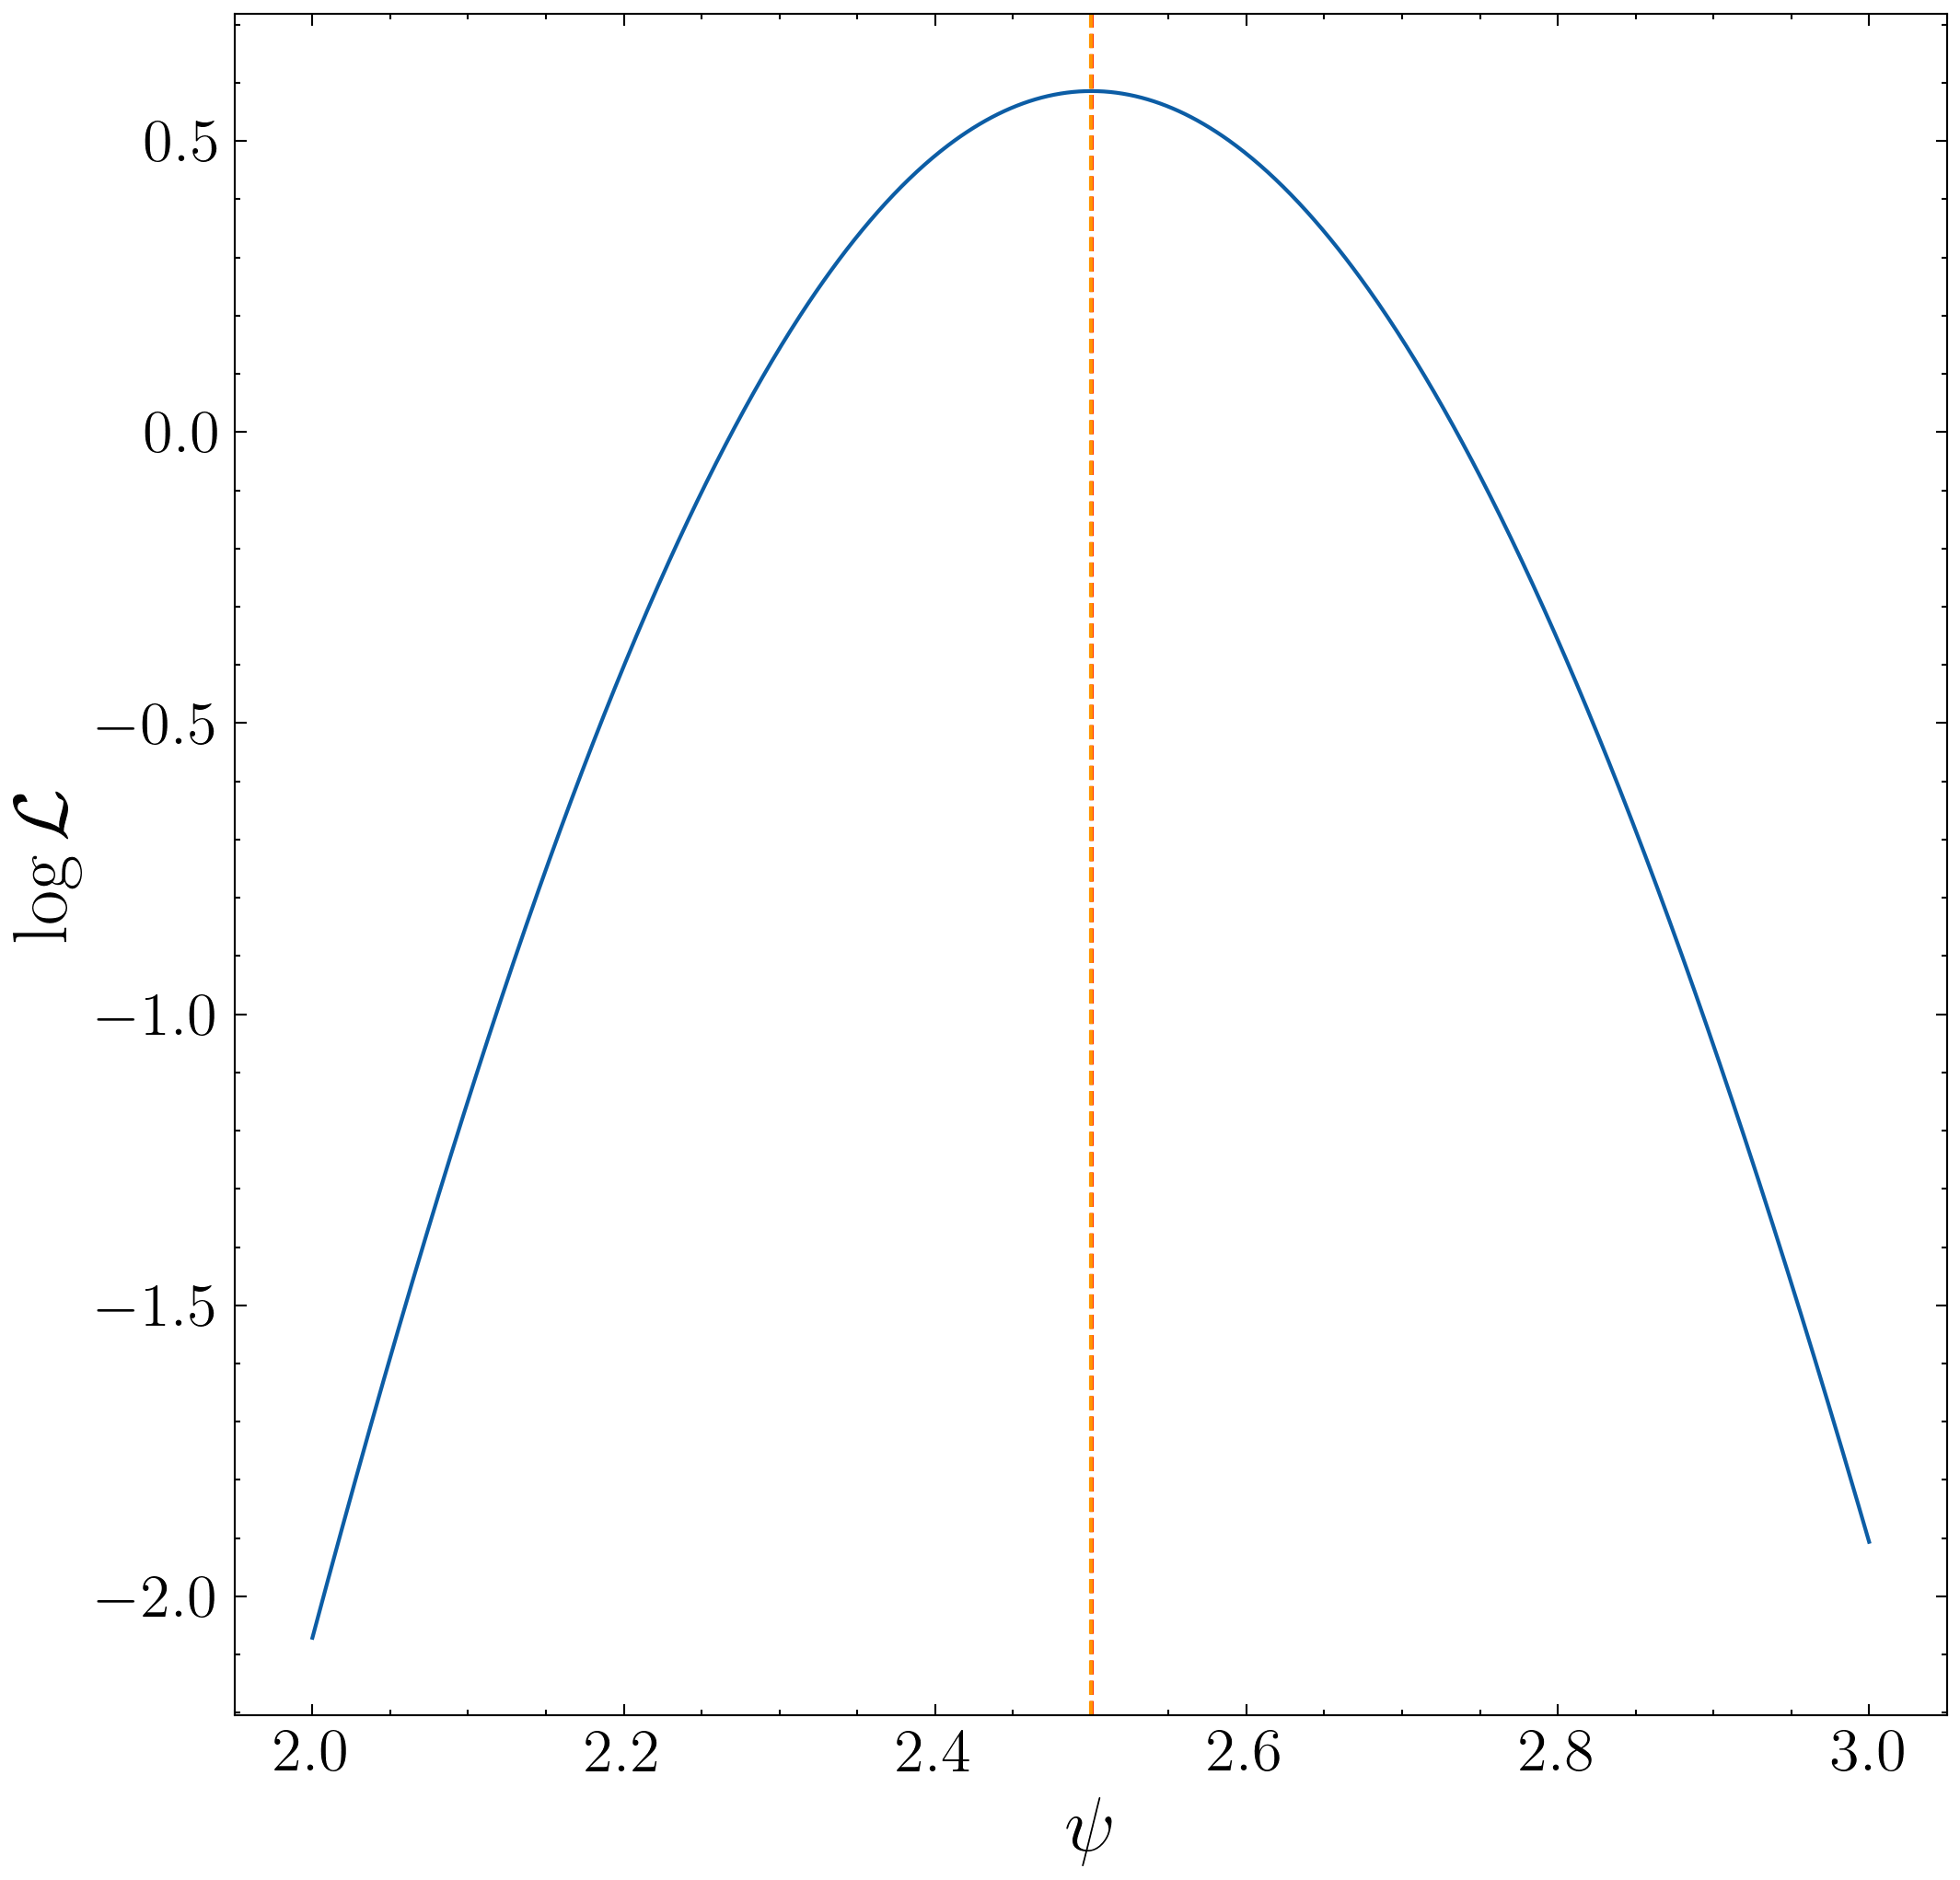
\includegraphics[width=\textwidth]{images/likelihood_psi_psr}
		\caption{$\psi$}
	\end{subfigure}
	\begin{subfigure}[b]{0.22\textwidth}
		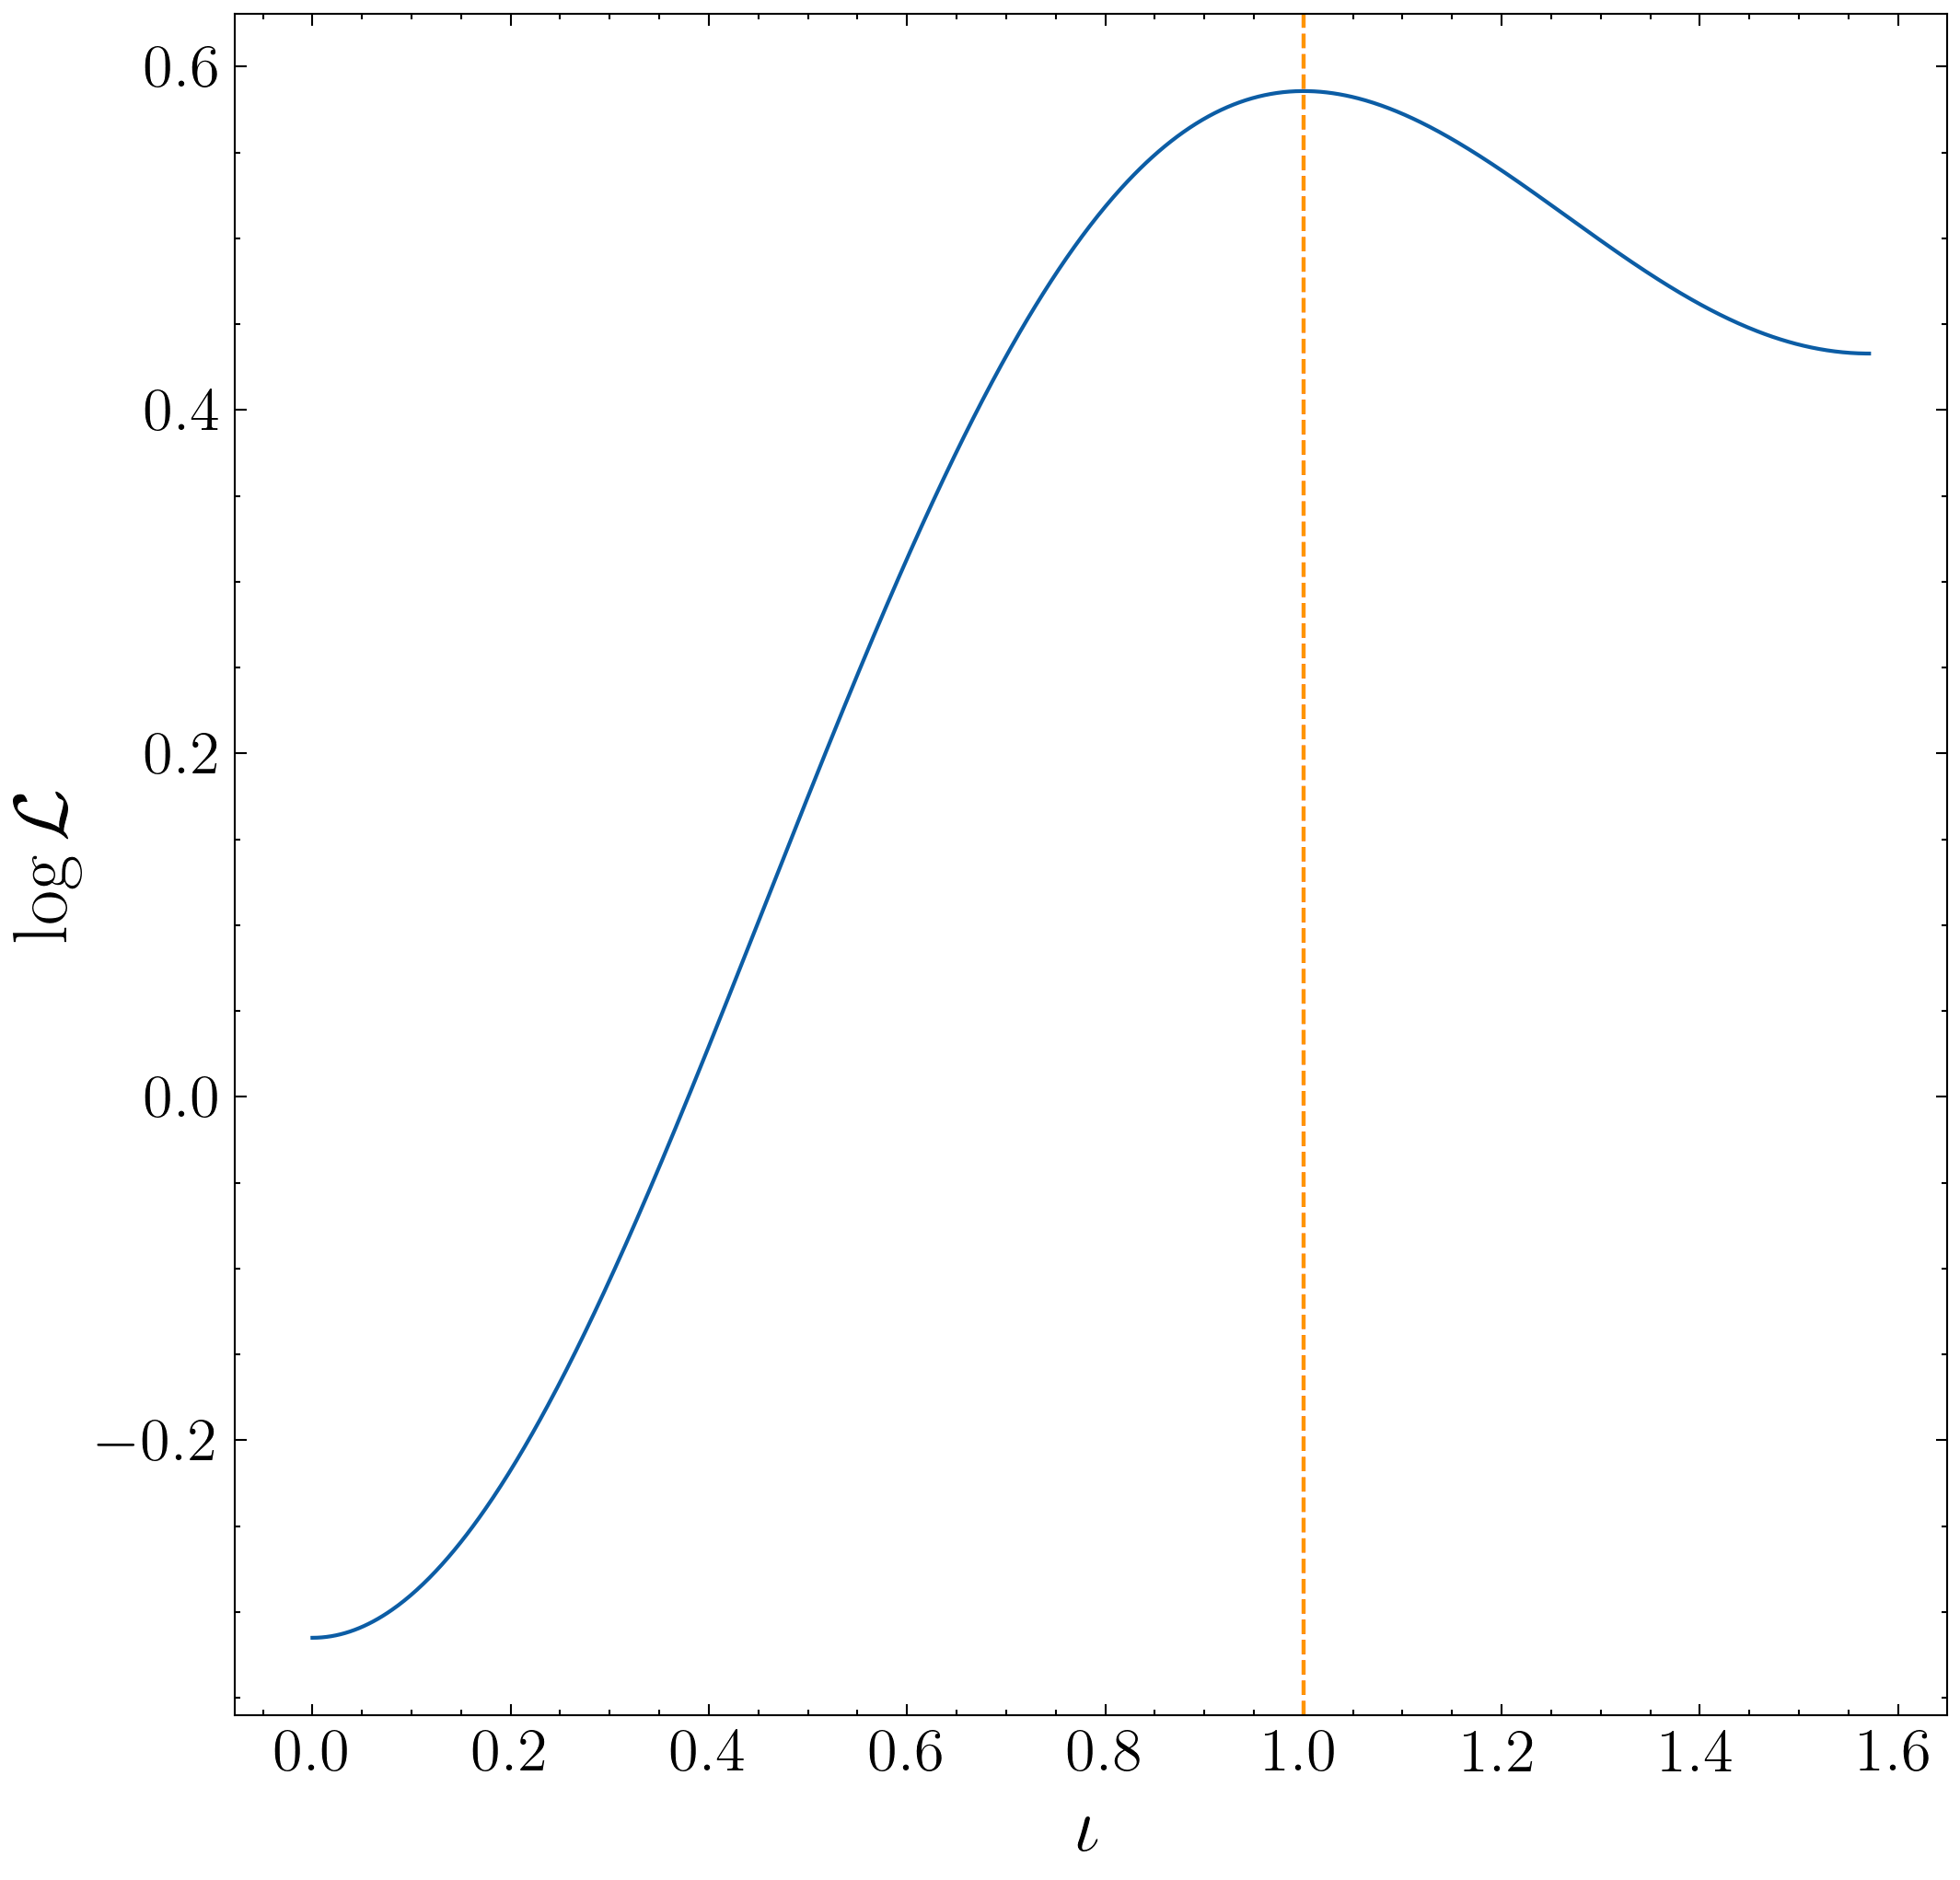
\includegraphics[width=\textwidth]{images/likelihood_iota_psr}
		\caption{$\iota$}
	\end{subfigure}
	\medskip
	\begin{subfigure}[b]{0.3\textwidth}
		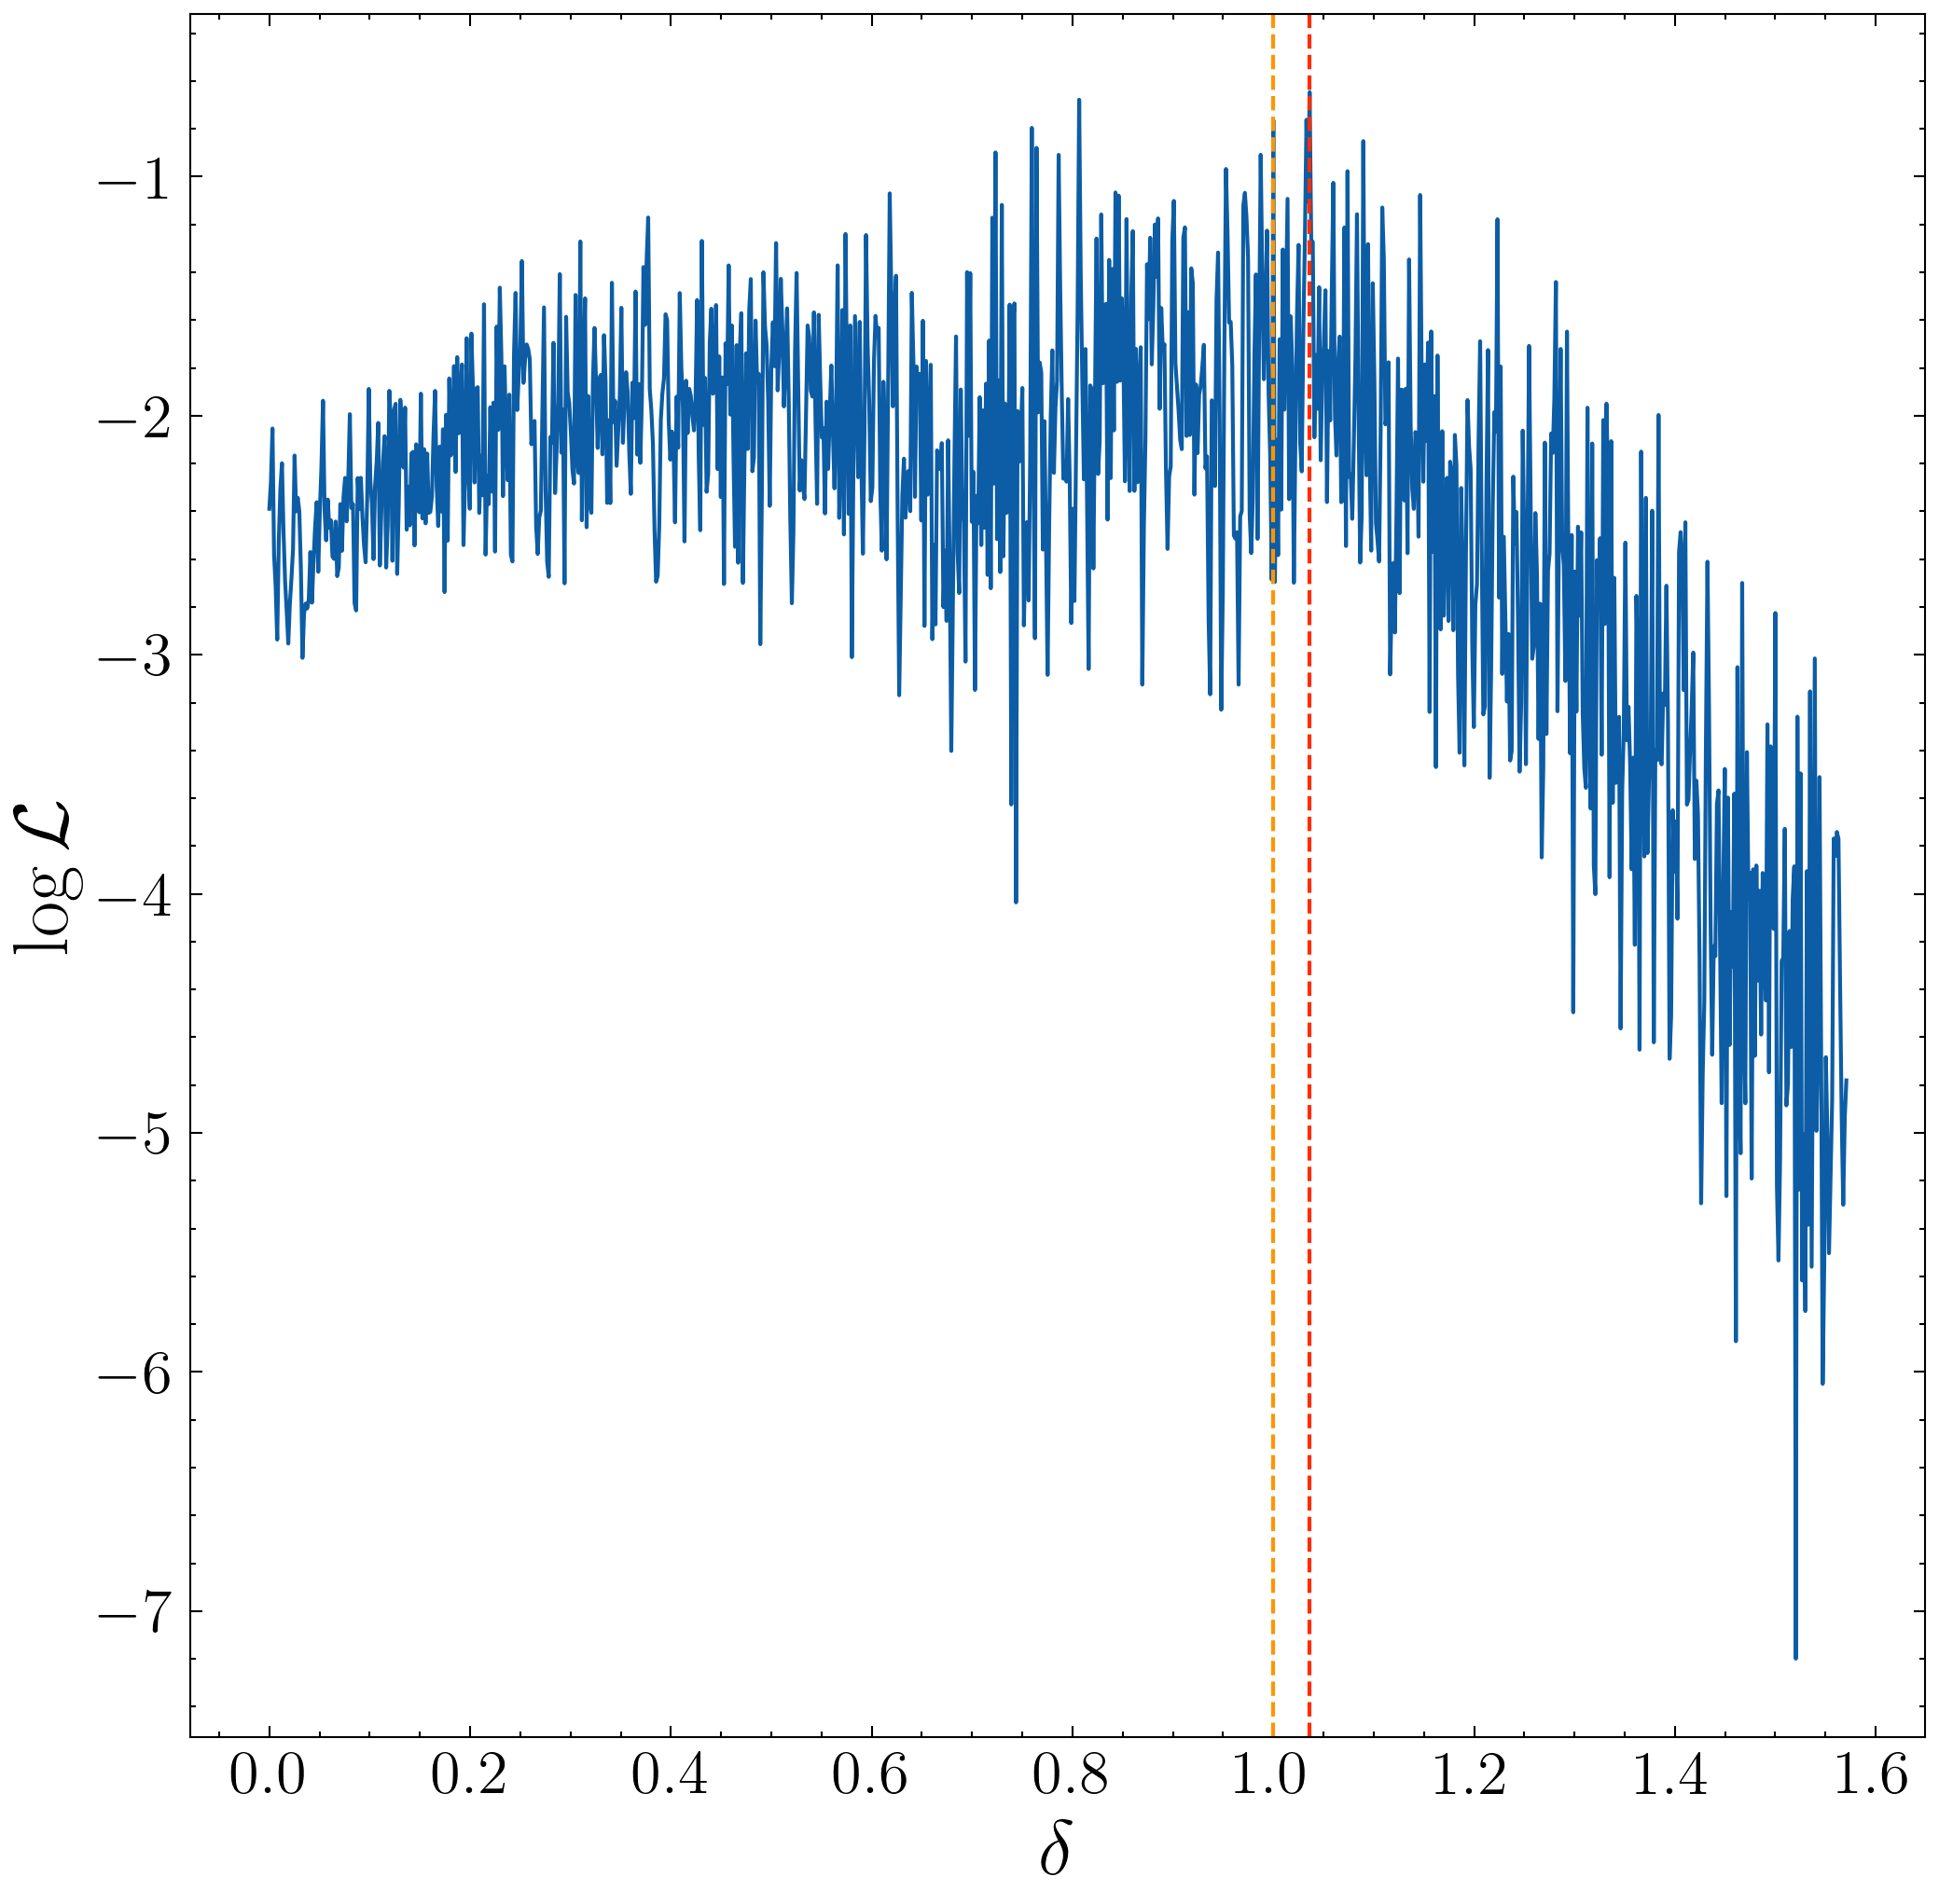
\includegraphics[width=\textwidth]{images/likelihood_delta_psr}
		\caption{$\delta$}
	\end{subfigure}
	\hfill
	\begin{subfigure}[b]{0.3\textwidth}
		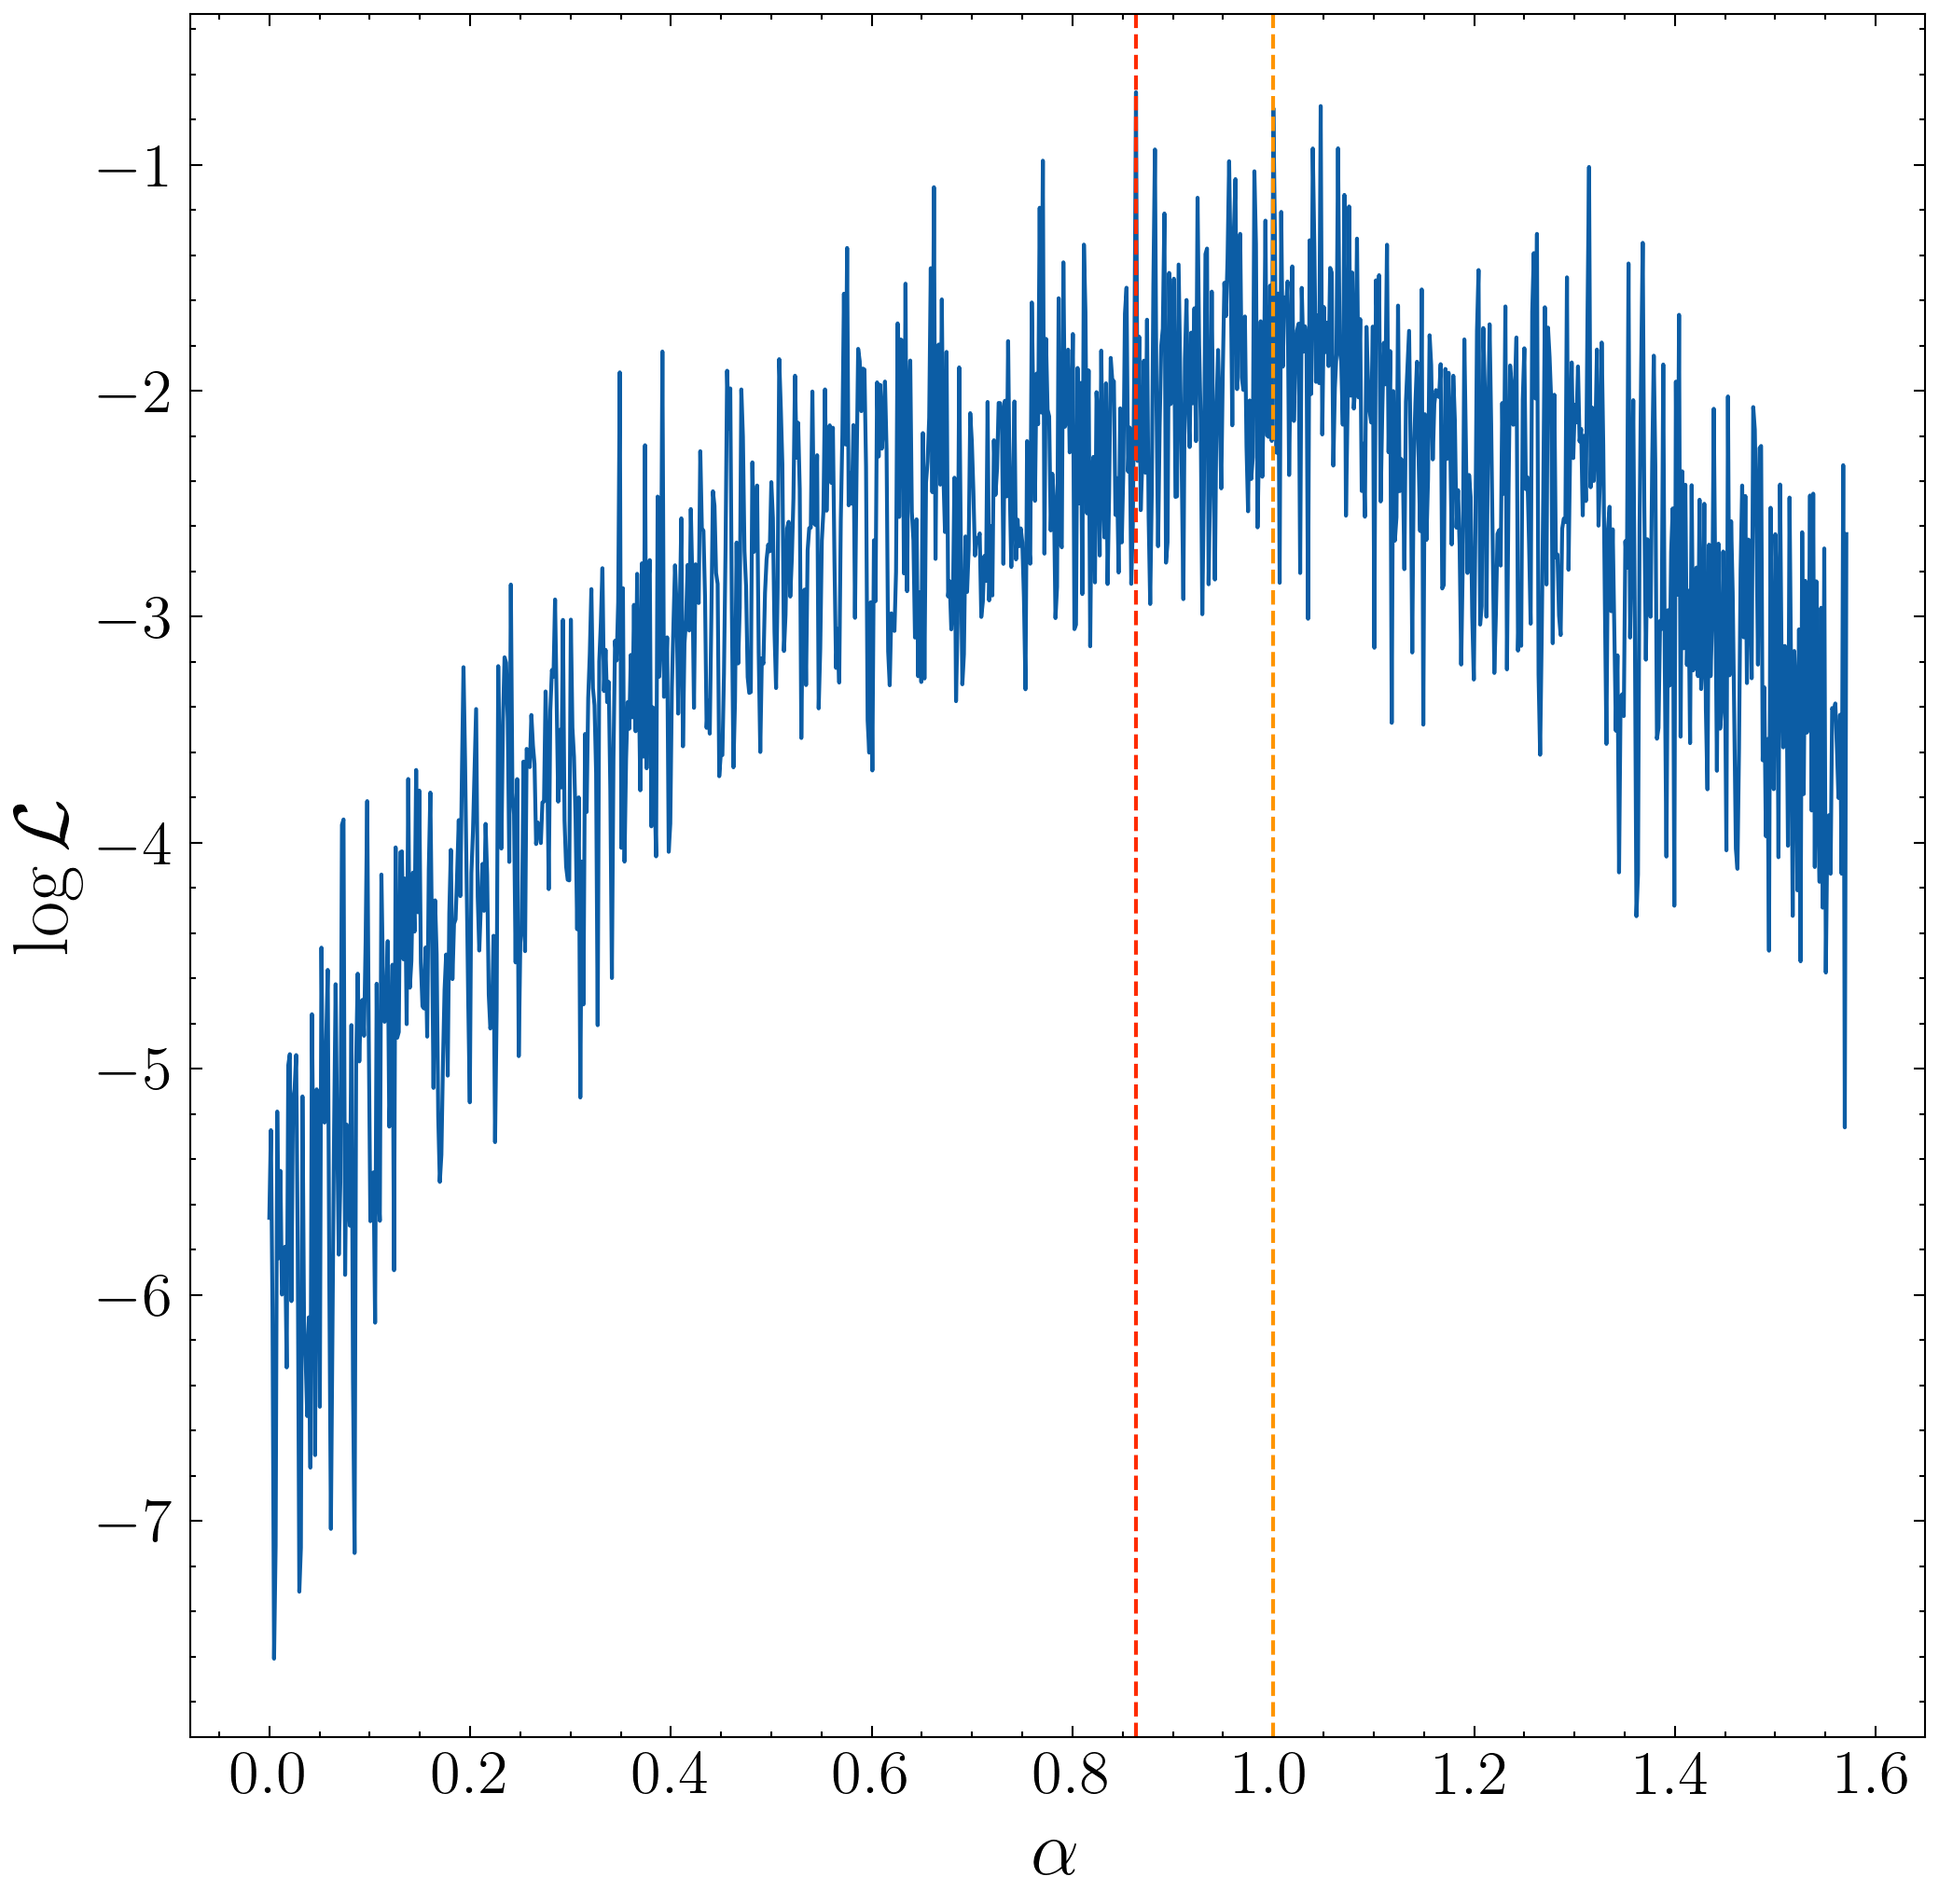
\includegraphics[width=\textwidth]{images/likelihood_alpha_psr}
		\caption{$\alpha$}
	\end{subfigure}
	\hfill
	\begin{subfigure}[b]{0.3\textwidth}
		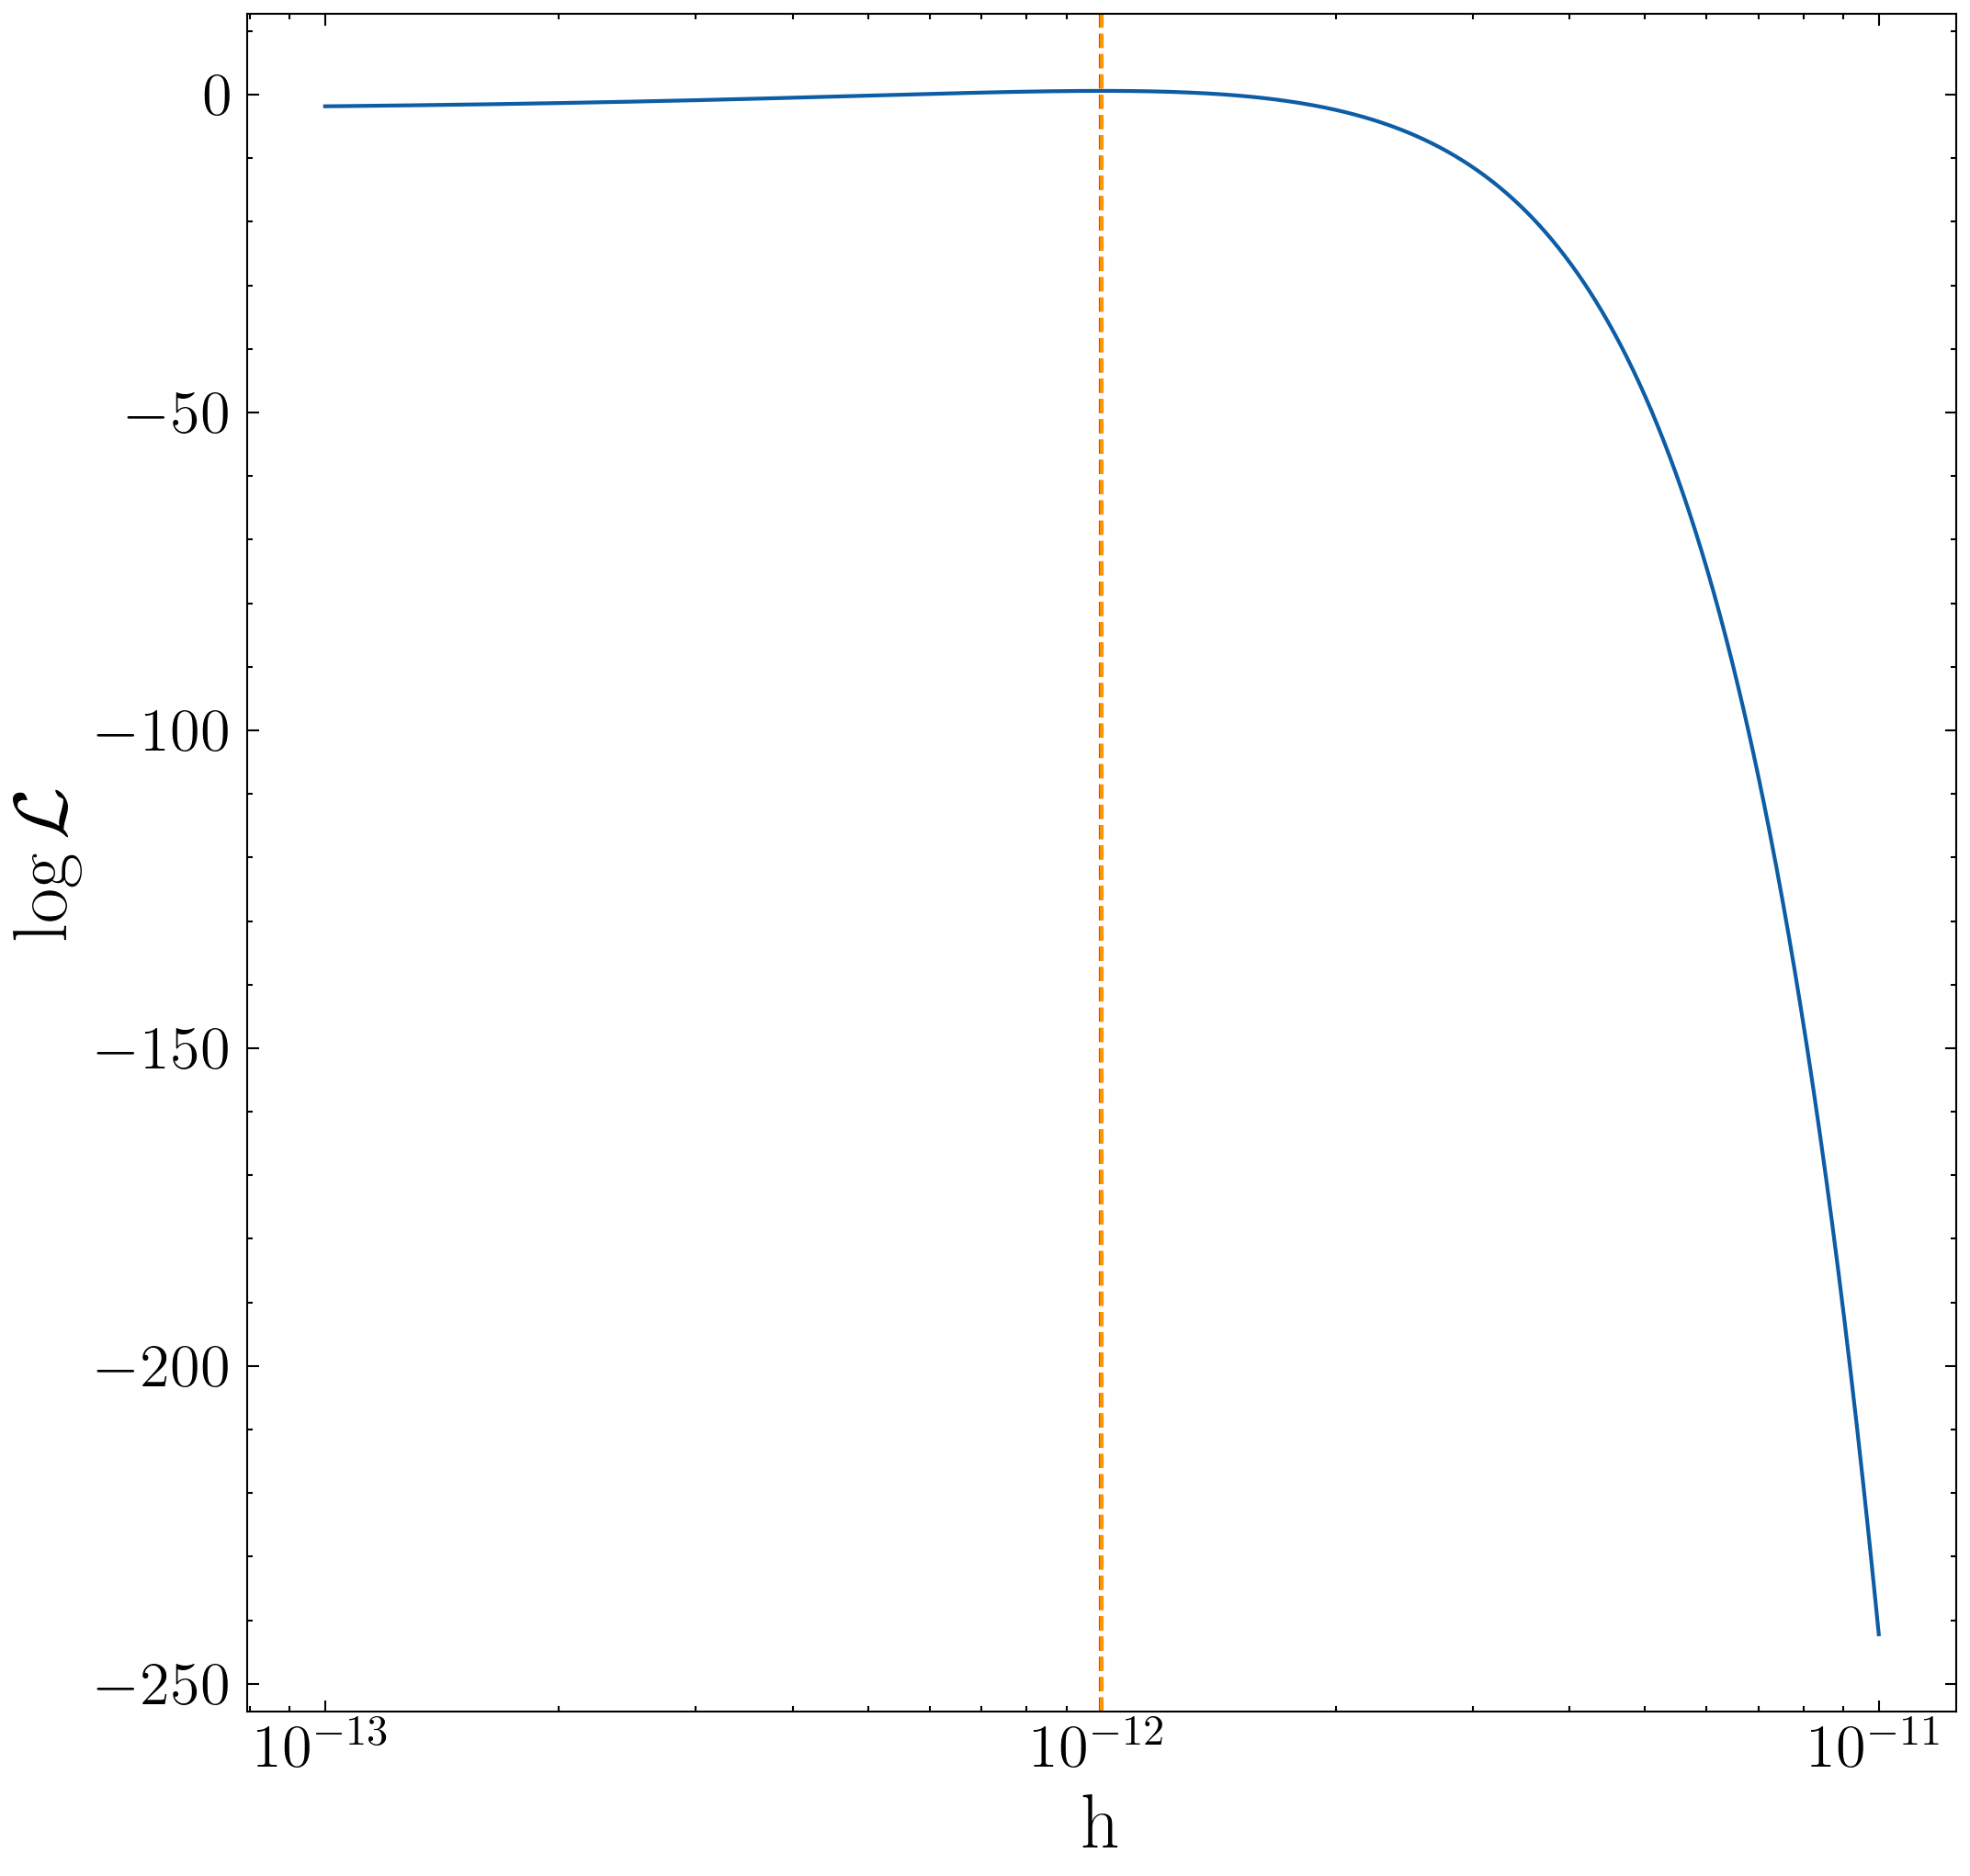
\includegraphics{images/likelihood_h_psr}
		\caption{$h$}
	\end{subfigure}
	
	\caption{As Figure \ref{fig:likelihood_curves_earth} but now including the pulsar terms in the measurement equation.}\label{fig:likelihood_curves_psr}
\end{figure*}


%\begin{figure*}
%	\centering
%	\subfigure[]{\includegraphics[width=0.24\textwidth]{example-image-a}} 
%	\subfigure[]{\includegraphics[width=0.24\textwidth]{example-image-a}} 
%	\subfigure[]{\includegraphics[width=0.24\textwidth]{example-image-a}}
%	\subfigure[]{\includegraphics[width=0.24\textwidth]{example-image-a}}
%	\caption{(a) blah (b) blah (c) blah (d) blah}
%	\label{fig:foobar}
%\end{figure*}


\section{Discussion}


Some potential further points for discussion


\begin{itemize}
	\item What is the performance of a single pulsar?
	\item How does this map to Hellings-downs?
	\item How does this map to having more than one source? Or a chrmomatic source?
	\item Non constant time sampling?
	\item Any further discussion on pulsar terms?
	\item PTAs like MSPs for small timing noise. Can we get away with large timing noise, and use more pulsars? Some pulsars are more useful than others, e.g. arXiv 2211.03201
	\item Can we also estimate radiometer noise? Is this useful?
\end{itemize}



\section{Conclusion}

\textcolor{red}{TK: TBD}




 \newpage 
\appendix

\section{Kalman recursion equations} \label{sec:kalman}




\textcolor{red}{TK: This section needs cleaning up}





The linear Kalman filter operates on temporally discrete measurements which are related to unobservable system states via a linear transformation
\begin{equation}
	\bar{z} = \bar{H} \bar{x} + \bar{v}
\end{equation}
where $\bar{H}$ is the measurement matrix and $\bar{v}$ is a Gaussian measurement noise. The underlying states evolve according to are the state-space dynamical equation 
\begin{equation}
	\dot{\bar{x}} = \bar{F} \bar{x} + \bar{G}\bar{u} + \bar{w}
\end{equation}
for the system dynamics matrix,$\bar{F}$,  control model $G$, control vector $\bar{u}$, and $w$ a stochastic zero-mean process. By comparison with the preceding equations, Eqs. 	\ref{eq:state1} - 	\ref{eq:state2}, it is immediately obvious how our state space model maps onto the Kalman filter structure. Specifically, our states are just the $N$ intrinsic pulsar frequencies $\bar{x} = (f_1,f_2,...f_N)$ whilst our measurements are the $N$ measured pulse frequencies $\bar{z} = (f^{(M)}_1,f^{(M)}_2,...f^{(M)}_N)$. If we specialize to the case of constant time sampling between our observations, $\Delta t$, then for our formulation the components that make up the Kalman filter are as follows: 
\begin{equation}
	F_i = F_{i+1} = e^{-\gamma \Delta t}
	\label{eq:fmatrix}
\end{equation}
\begin{align}
	T_i &= \int_{t_i}^{t_{i+1}}  e^{A (t_{i+1} - t')} N(t') dt' \\
	& = f_{\rm EM}(0) + \dot{f}_{\rm EM}(0)  (\Delta t + t_i) - e^{-\gamma \Delta t} (f_{\rm EM}(0) + \dot{f}_{\rm EM}(0)t_i)
\end{align}
\begin{equation}
	H_i = 1 -A(\theta_{\rm GW}) \cos(-\Omega t_i (1 + n\cdot q ) + \Phi_0)
\end{equation}
where the $i$ subscript labels the value at the $i$-th timestep, and $A$ is a constant that is given by  Eq. \ref{eq:state2}. \newline 


\noindent The Kalman filter includes the effect of process noise $\bar{w}$ and the measurement noise $\bar{v}$ via the definition of a process noise matrix $Q = E[w w^T]$ and a measurement noise matrix $R = E[v v^T]$, which have the discrete form,
\begin{equation}
	Q_i  \delta_{ij}= \langle \eta_i \eta_j^T \rangle = \frac{- \sigma^2}{2 \gamma} \left( e^{-2 \gamma \Delta t} -1\right)
\end{equation}
\begin{equation}
	R_i = R_{i+1} = \Sigma^2
	\label{eq:rmatix}
\end{equation}
The above equations, Eqs. \ref{eq:fmatrix} - 	\ref{eq:rmatix}, apply to an operation on a single state. The extension to $N$ states is straightforward, since one just needs to construct a diagonal matrix for each of the Kalman components where each non-zero element corresponds to a separate pulsar frequency. 





In Section \ref{sec:statespace} we present a discretised version of the model of Section \ref{sec:model} which maps onto the discretely sampled observable $f(\tau)|_{\rm Earth}$. 





In order to make contact with discretely sampled data it is importnat to temporally discretise the model of Section \ref{sec:model}


We can express the intrinsic frequency evolution, Eq. \ref{eq:frequency_evolution_expanded}, in a alternative form as,
\textcolor{red}{TK all this needs updating}
\begin{equation}
	df = \gamma  f dt + N(t) dt + \sigma dB(t)
	\label{eq:state1}
\end{equation}
where $\mathcal{A} = -\gamma$, $N(t) = \gamma(f_{\rm EM}(0) + \dot{f}_{\rm EM}(0) t) +\dot{f}_{\rm EM}(0)$ and $dB(t)$ denotes increments of Brownian motion (Wiener process). This equation is easily identified as an Ornstein-Uhlenbeck process which has a general solution given by \citep{gardiner2009stochastic},
\begin{equation}
	f(t) = e^{\mathcal{A}t}f(0) + \int_0^t e^{\mathcal{A}(t-t')} N(t') dt' + \int_0^t e^{\mathcal{A}(t-t')} \sigma dB(t')
\end{equation} 
If we move from a solution in continuous time, $t$, to discrete time, \textcolor{red}{TK: AM reccomends deligint tabe sy,bol} $\bar{t} = (t_1, t_2, ...,t_K)$, then
\begin{equation}
	f(t_{i+1}) = F f(t_i) + T_i + \eta_i
\end{equation}
where
\begin{equation}
	F_i = e^{\mathcal{A} (t_{i+1} - t_i)}
\end{equation}
\begin{equation}
	T_i = \int_{t_i}^{t_{i+1}}  e^{\mathcal{A} (t_{i+1} - t')} N(t') \, dt'
\end{equation}
\begin{equation}
	\eta_i = \int_{t_i}^{t_{i+1}}  e^{\mathcal{A} (t_{i+1} - t')} \sigma \, dt'
\end{equation}

if we specialise to the case of constatn time sampling 






The discrete solution $f(\bar{t})$ to the intrinsic frequency can be related to the discrete measured frequency via Eq. \ref{eq:main_eq} as,
\begin{equation}
	f_M (\bar{t})= f(\bar{t}) g(\bar{\theta},\bar{t}) + N_M
\end{equation}
where $g(\theta,t)$ can be expressed in a trigonometric form as 
\begin{equation}
	X = 1 - \frac{1}{2} \frac{ H_{ij}q^i q^j }{(1 + \bar{n}\cdot \bar{q}) } \left[ \cos(-\Omega \tau +\Phi_0) - \cos(-\Omega \tau +\Phi_0 + \Omega (1 + \bar{n}\cdot \bar{q})  d) \right]
\end{equation} 
whilst $N_M$ is a Gaussian measurement noise that satisfies 
\begin{equation}
	\langle N_M(t) N_M(t') \rangle = \Sigma^2 \delta(t - t')
\end{equation}
for variance $\Sigma^2$. 









\subsection{References}
\label{sec:ref_list}





\bibliographystyle{mnras}
\bibliography{example} % if your bibtex file is called example.bib





%%%%%%%%%%%%%%%%%%%%%%%%%%%%%%%%%%%%%%%%%%%%%%%%%%


% Don't change these lines
\bsp	% typesetting comment
\label{lastpage}
\end{document}

% End of mnras_guide.tex
